\documentclass[]{book}
\usepackage{lmodern}
\usepackage{amssymb,amsmath}
\usepackage{ifxetex,ifluatex}
\usepackage{fixltx2e} % provides \textsubscript
\ifnum 0\ifxetex 1\fi\ifluatex 1\fi=0 % if pdftex
  \usepackage[T1]{fontenc}
  \usepackage[utf8]{inputenc}
\else % if luatex or xelatex
  \ifxetex
    \usepackage{mathspec}
  \else
    \usepackage{fontspec}
  \fi
  \defaultfontfeatures{Ligatures=TeX,Scale=MatchLowercase}
\fi
% use upquote if available, for straight quotes in verbatim environments
\IfFileExists{upquote.sty}{\usepackage{upquote}}{}
% use microtype if available
\IfFileExists{microtype.sty}{%
\usepackage{microtype}
\UseMicrotypeSet[protrusion]{basicmath} % disable protrusion for tt fonts
}{}
\usepackage[margin=1in]{geometry}
\usepackage{hyperref}
\hypersetup{unicode=true,
            pdftitle={Managing Batch Effects in Microbiome Data},
            pdfauthor={Yiwen Wang, Kim-Anh Lê Cao},
            pdfborder={0 0 0},
            breaklinks=true}
\urlstyle{same}  % don't use monospace font for urls
\usepackage{natbib}
\bibliographystyle{apalike}
\usepackage{color}
\usepackage{fancyvrb}
\newcommand{\VerbBar}{|}
\newcommand{\VERB}{\Verb[commandchars=\\\{\}]}
\DefineVerbatimEnvironment{Highlighting}{Verbatim}{commandchars=\\\{\}}
% Add ',fontsize=\small' for more characters per line
\usepackage{framed}
\definecolor{shadecolor}{RGB}{248,248,248}
\newenvironment{Shaded}{\begin{snugshade}}{\end{snugshade}}
\newcommand{\KeywordTok}[1]{\textcolor[rgb]{0.13,0.29,0.53}{\textbf{#1}}}
\newcommand{\DataTypeTok}[1]{\textcolor[rgb]{0.13,0.29,0.53}{#1}}
\newcommand{\DecValTok}[1]{\textcolor[rgb]{0.00,0.00,0.81}{#1}}
\newcommand{\BaseNTok}[1]{\textcolor[rgb]{0.00,0.00,0.81}{#1}}
\newcommand{\FloatTok}[1]{\textcolor[rgb]{0.00,0.00,0.81}{#1}}
\newcommand{\ConstantTok}[1]{\textcolor[rgb]{0.00,0.00,0.00}{#1}}
\newcommand{\CharTok}[1]{\textcolor[rgb]{0.31,0.60,0.02}{#1}}
\newcommand{\SpecialCharTok}[1]{\textcolor[rgb]{0.00,0.00,0.00}{#1}}
\newcommand{\StringTok}[1]{\textcolor[rgb]{0.31,0.60,0.02}{#1}}
\newcommand{\VerbatimStringTok}[1]{\textcolor[rgb]{0.31,0.60,0.02}{#1}}
\newcommand{\SpecialStringTok}[1]{\textcolor[rgb]{0.31,0.60,0.02}{#1}}
\newcommand{\ImportTok}[1]{#1}
\newcommand{\CommentTok}[1]{\textcolor[rgb]{0.56,0.35,0.01}{\textit{#1}}}
\newcommand{\DocumentationTok}[1]{\textcolor[rgb]{0.56,0.35,0.01}{\textbf{\textit{#1}}}}
\newcommand{\AnnotationTok}[1]{\textcolor[rgb]{0.56,0.35,0.01}{\textbf{\textit{#1}}}}
\newcommand{\CommentVarTok}[1]{\textcolor[rgb]{0.56,0.35,0.01}{\textbf{\textit{#1}}}}
\newcommand{\OtherTok}[1]{\textcolor[rgb]{0.56,0.35,0.01}{#1}}
\newcommand{\FunctionTok}[1]{\textcolor[rgb]{0.00,0.00,0.00}{#1}}
\newcommand{\VariableTok}[1]{\textcolor[rgb]{0.00,0.00,0.00}{#1}}
\newcommand{\ControlFlowTok}[1]{\textcolor[rgb]{0.13,0.29,0.53}{\textbf{#1}}}
\newcommand{\OperatorTok}[1]{\textcolor[rgb]{0.81,0.36,0.00}{\textbf{#1}}}
\newcommand{\BuiltInTok}[1]{#1}
\newcommand{\ExtensionTok}[1]{#1}
\newcommand{\PreprocessorTok}[1]{\textcolor[rgb]{0.56,0.35,0.01}{\textit{#1}}}
\newcommand{\AttributeTok}[1]{\textcolor[rgb]{0.77,0.63,0.00}{#1}}
\newcommand{\RegionMarkerTok}[1]{#1}
\newcommand{\InformationTok}[1]{\textcolor[rgb]{0.56,0.35,0.01}{\textbf{\textit{#1}}}}
\newcommand{\WarningTok}[1]{\textcolor[rgb]{0.56,0.35,0.01}{\textbf{\textit{#1}}}}
\newcommand{\AlertTok}[1]{\textcolor[rgb]{0.94,0.16,0.16}{#1}}
\newcommand{\ErrorTok}[1]{\textcolor[rgb]{0.64,0.00,0.00}{\textbf{#1}}}
\newcommand{\NormalTok}[1]{#1}
\usepackage{longtable,booktabs}
\usepackage{graphicx,grffile}
\makeatletter
\def\maxwidth{\ifdim\Gin@nat@width>\linewidth\linewidth\else\Gin@nat@width\fi}
\def\maxheight{\ifdim\Gin@nat@height>\textheight\textheight\else\Gin@nat@height\fi}
\makeatother
% Scale images if necessary, so that they will not overflow the page
% margins by default, and it is still possible to overwrite the defaults
% using explicit options in \includegraphics[width, height, ...]{}
\setkeys{Gin}{width=\maxwidth,height=\maxheight,keepaspectratio}
\IfFileExists{parskip.sty}{%
\usepackage{parskip}
}{% else
\setlength{\parindent}{0pt}
\setlength{\parskip}{6pt plus 2pt minus 1pt}
}
\setlength{\emergencystretch}{3em}  % prevent overfull lines
\providecommand{\tightlist}{%
  \setlength{\itemsep}{0pt}\setlength{\parskip}{0pt}}
\setcounter{secnumdepth}{5}
% Redefines (sub)paragraphs to behave more like sections
\ifx\paragraph\undefined\else
\let\oldparagraph\paragraph
\renewcommand{\paragraph}[1]{\oldparagraph{#1}\mbox{}}
\fi
\ifx\subparagraph\undefined\else
\let\oldsubparagraph\subparagraph
\renewcommand{\subparagraph}[1]{\oldsubparagraph{#1}\mbox{}}
\fi

%%% Use protect on footnotes to avoid problems with footnotes in titles
\let\rmarkdownfootnote\footnote%
\def\footnote{\protect\rmarkdownfootnote}

%%% Change title format to be more compact
\usepackage{titling}

% Create subtitle command for use in maketitle
\newcommand{\subtitle}[1]{
  \posttitle{
    \begin{center}\large#1\end{center}
    }
}

\setlength{\droptitle}{-2em}

  \title{Managing Batch Effects in Microbiome Data}
    \pretitle{\vspace{\droptitle}\centering\huge}
  \posttitle{\par}
    \author{Yiwen Wang, Kim-Anh Lê Cao}
    \preauthor{\centering\large\emph}
  \postauthor{\par}
      \predate{\centering\large\emph}
  \postdate{\par}
    \date{2019-10-22}

\usepackage{booktabs}
\usepackage{amsthm}
\makeatletter
\def\thm@space@setup{%
  \thm@preskip=8pt plus 2pt minus 4pt
  \thm@postskip=\thm@preskip
}
\makeatother


\usepackage{fancyhdr}
\usepackage{hyperref}
\usepackage{lipsum}
\setlength{\headheight}{28pt}
\setlength{\footskip}{25pt}
\pagestyle{fancy}
\renewcommand{\headrulewidth}{0.5pt}
\renewcommand{\footrulewidth}{0.5pt}
\lhead{
\includegraphics[width=10cm,height=1.5cm]{logo-unimelb}}
\cfoot{\scriptsize Vignette | School of Math \& Stats, Melbourne Integrative Genomics, University of Melbourne}
\rfoot{\scriptsize \thepage}
\fancyhead[R]{\slshape\leftmark}
\fancypagestyle{plain}{\pagestyle{fancy}}

\usepackage{fontspec}
\setmainfont{Times New Roman}

\begin{document}
\maketitle

{
\setcounter{tocdepth}{3}
\tableofcontents
}
\chapter{Examples of microbiome studies with batch
effects}\label{examples-of-microbiome-studies-with-batch-effects}

This vignette provides all the analyses performed in the paper `Managing
Batch Effects in Microbiome Data' by Yiwen Wang and Kim-Anh Lê Cao.

\textbf{Packages installation and loading}

First, you will need to install then load the following packages from
the CRAN and Bioconductor:

\begin{Shaded}
\begin{Highlighting}[]
\CommentTok{# cran.packages <- c('knitr', 'mixOmics', 'xtable', 'ggplot2', 'vegan', 'cluster',}
\CommentTok{#                   'gridExtra', 'pheatmap', 'ruv', 'lmerTest', 'bapred')}
\CommentTok{# install.packages(cran.packages)}
\CommentTok{# bioconductor.packages <- c('sva', 'limma', 'AgiMicroRna', }
\CommentTok{#                           'variancePartition', 'pvca')}
\CommentTok{# if (!requireNamespace('BiocManager', quietly = TRUE))}
\CommentTok{#     install.packages('BiocManager')}
\CommentTok{# BiocManager::install(bioconductor.packages, version = '3.8')}

\KeywordTok{library}\NormalTok{(knitr)}
\KeywordTok{library}\NormalTok{(xtable) }\CommentTok{# table}
\KeywordTok{library}\NormalTok{(mixOmics)}
\KeywordTok{library}\NormalTok{(sva) }\CommentTok{# ComBat}
\KeywordTok{library}\NormalTok{(ggplot2) }\CommentTok{# PCA sample plot with density}
\KeywordTok{library}\NormalTok{(gridExtra) }\CommentTok{# PCA sample plot with density}
\KeywordTok{library}\NormalTok{(limma) }\CommentTok{# removeBatchEffect (LIMMA)}
\KeywordTok{library}\NormalTok{(vegan) }\CommentTok{# RDA}
\KeywordTok{library}\NormalTok{(AgiMicroRna) }\CommentTok{# RLE plot}
\KeywordTok{library}\NormalTok{(cluster) }\CommentTok{# silhouette coefficient}
\KeywordTok{library}\NormalTok{(variancePartition) }\CommentTok{# variance calculation}
\KeywordTok{library}\NormalTok{(pvca) }\CommentTok{# PVCA}
\KeywordTok{library}\NormalTok{(pheatmap) }\CommentTok{# heatmap}
\KeywordTok{library}\NormalTok{(ruv) }\CommentTok{# RUVIII}
\KeywordTok{library}\NormalTok{(lmerTest) }\CommentTok{# lmer}
\KeywordTok{library}\NormalTok{(bapred) }\CommentTok{# FAbatch}
\end{Highlighting}
\end{Shaded}

\section{Study description}\label{study-description}

\subsection{\texorpdfstring{Sponge \emph{Aplysina aerophoba}
study}{Sponge Aplysina aerophoba study}}\label{sponge-aplysina-aerophoba-study}

Sacristán-Soriano \emph{et al.} studied the potential involvement of
bacterial communities from the sponge species \emph{A. aerophoba} in the
biosynthesis of brominated alkaloids (BAs)
\citep{sacristan2011exploring}. They compared the microbial composition
and BA concentration in two different tissues (ectosome and choanosome)
to investigate the relationship between bacterial composition and BA
concentration. The authors concluded that differences in bacterial
profiles were not only due to tissue variation (the main effect of
interest), but also because the samples were run on two separate
denaturing gradient gels during processing. Gel thus acted as a
technical batch effect as described in Table 1 below.

\textbf{Table 1. Overview of exemplar datasets with batch effects.} We
considered microbiome studies from sponge \emph{Aplysina aerophoba};
organic matter in anaerobic digestion (AD) and mice models with
Huntington's disease (HD).

\begin{center}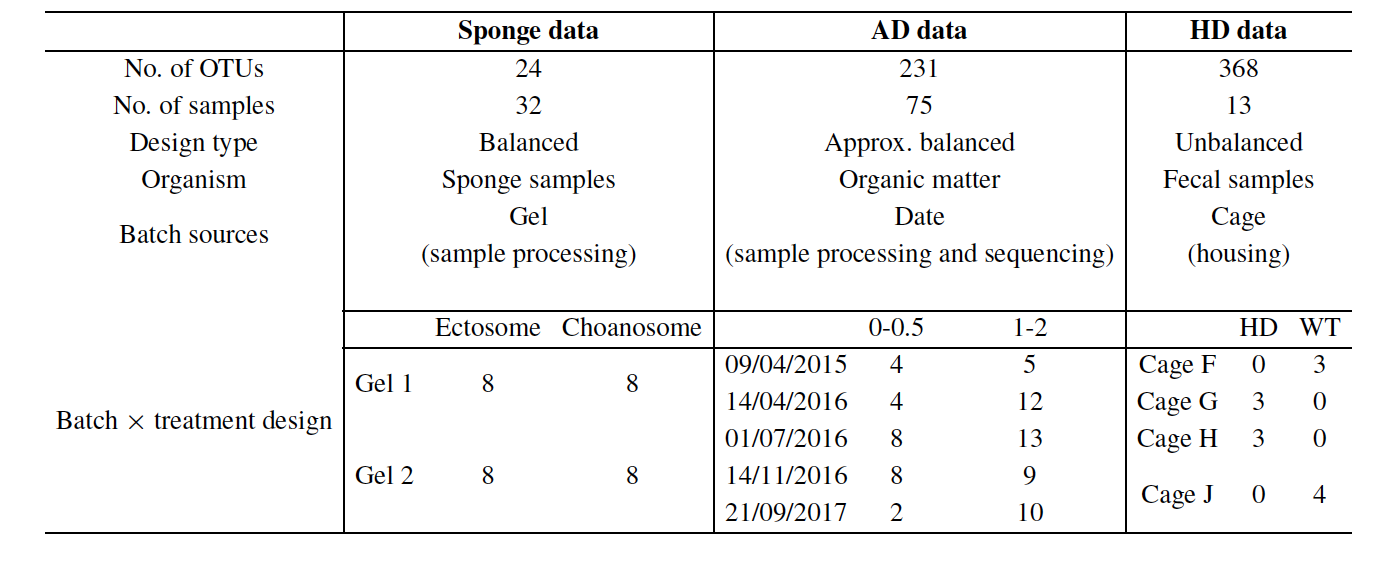
\includegraphics{figures/table} \end{center}

\subsection{Anaerobic digestion study}\label{anaerobic-digestion-study}

Anaerobic Digestion (AD) is a microbiological process of organic matter
degradation that produces a biogas used in electrical and thermal energy
production. However, the AD bioprocess undergoes inhibition during its
developmental stage that is not well characterised: Chapleur \emph{et
al.} explored microbial indicators that could improve the AD
bioprocess's efficacy and prevent its failure
\citep{chapleur2016increasing}. They profiled the microbiota of 75 AD
samples in various conditions. Here we consider two different ranges of
phenol concentration as treatments. The experiment was conducted at
different dates (5), which constitutes a technical source of unwanted
variation (Table 1).

\subsection{Huntington's disease study}\label{huntingtons-disease-study}

In their study, Kong \emph{et al.} reported differences in microbial
composition between Huntington's disease (HD) and wild-type (WT) mice
\citep{kong2018microbiome}. However, the establishment of microbial
communities was also driven by biological batch effects: the cage
environment and sex. Here we consider only female mice to illustrate a
special case of a batch \(\times\) treatment unbalanced design. The HD
data include 13 faecal mice samples hosted across 4 cages (Table 1).

We load the data and functions that are provided \emph{outside} the
packages.

\begin{Shaded}
\begin{Highlighting}[]
\CommentTok{# load the data}
\KeywordTok{load}\NormalTok{(}\DataTypeTok{file =} \StringTok{'./datasets/microbiome_datasets.RData'}\NormalTok{)}

\CommentTok{# load the extra functions}
\KeywordTok{source}\NormalTok{(}\DataTypeTok{file =} \StringTok{'./Functions.R'}\NormalTok{)}
\KeywordTok{dim}\NormalTok{(sponge.tss)}
\end{Highlighting}
\end{Shaded}

\begin{verbatim}
## [1] 32 24
\end{verbatim}

\begin{Shaded}
\begin{Highlighting}[]
\KeywordTok{dim}\NormalTok{(ad.count)}
\end{Highlighting}
\end{Shaded}

\begin{verbatim}
## [1]  75 567
\end{verbatim}

\begin{Shaded}
\begin{Highlighting}[]
\KeywordTok{dim}\NormalTok{(hd.count)}
\end{Highlighting}
\end{Shaded}

\begin{verbatim}
## [1]  13 368
\end{verbatim}

\textbf{Note:} the AD data and HD data loaded are raw counts, while
sponge data are total sum scaling (TSS) scaled data calculated on raw
counts, with no offset.

\section{Data processing}\label{data-processing}

Here are the processing steps for the \textbf{raw count} microbiome
data:

\begin{enumerate}
\def\labelenumi{\arabic{enumi}.}
\tightlist
\item
  Prefilter the count data to remove features with excess zeroes across
  all samples\\
\item
  Add an offset of 1 to the whole data matrix --- note that this is not
  ideal but provides a pracitical way to handle zero counts.\\
\item
  Log-ratio transformation with Centered Log Ratio (CLR)
\end{enumerate}

\subsection{Prefiltering}\label{prefiltering}

We use a prefiltering step to remove OTUs for which the sum of counts
are below a set threshold (0.01\%) compared to the total sum of all
counts \citep{arumugam2011enterotypes}.

\begin{Shaded}
\begin{Highlighting}[]
\CommentTok{# ad data}
\NormalTok{ad.index.keep <-}\StringTok{ }\KeywordTok{which}\NormalTok{(}\KeywordTok{colSums}\NormalTok{(ad.count)}\OperatorTok{*}\DecValTok{100}\OperatorTok{/}\NormalTok{(}\KeywordTok{sum}\NormalTok{(}\KeywordTok{colSums}\NormalTok{(ad.count))) }\OperatorTok{>}\StringTok{ }\FloatTok{0.01}\NormalTok{)}
\NormalTok{ad.count.keep <-}\StringTok{ }\NormalTok{ad.count[, ad.index.keep]}
\KeywordTok{dim}\NormalTok{(ad.count.keep)}
\end{Highlighting}
\end{Shaded}

\begin{verbatim}
## [1]  75 231
\end{verbatim}

\begin{Shaded}
\begin{Highlighting}[]
\CommentTok{# hd data}
\NormalTok{hd.count.keep <-}\StringTok{ }\NormalTok{hd.count}
\KeywordTok{dim}\NormalTok{(hd.count.keep)}
\end{Highlighting}
\end{Shaded}

\begin{verbatim}
## [1]  13 368
\end{verbatim}

\textbf{Note:} The HD data only include 13 samples, which are a small
part of a big dataset that has already been prefiltered. We retained all
the OTUs in the data and did not redo the prefiltering again.

\subsection{Adding offset}\label{adding-offset}

We need to add an offset of 1 to all count data to handle zeroes for the
CLR transformation. As the sponge data were TSS scaled, a small offset
is added in this specific case. According to scale invariance principle
\citep{aitchison1986statistical}, it returns the same results with CLR
transformation on raw counts or TSS data. However, we recommend starting
from the raw counts (not TSS) for those analyses.

\begin{Shaded}
\begin{Highlighting}[]
\CommentTok{# sponge data}
\NormalTok{sponge.tss <-}\StringTok{ }\NormalTok{sponge.tss }\OperatorTok{+}\StringTok{ }\FloatTok{0.01}

\CommentTok{# ad data}
\NormalTok{ad.count.keep <-}\StringTok{ }\NormalTok{ad.count.keep }\OperatorTok{+}\StringTok{ }\DecValTok{1}

\CommentTok{# hd data}
\NormalTok{hd.count.keep <-}\StringTok{ }\NormalTok{hd.count.keep }\OperatorTok{+}\StringTok{ }\DecValTok{1}
\end{Highlighting}
\end{Shaded}

\subsection{Centered log-ratio
transformation}\label{centered-log-ratio-transformation}

Microbiome data are compostional and with different library sizes. Using
standard statistical methods on such data may lead to spurious results
and therefore the data must be further transformed. The CLR is the
transformation of choice.

\begin{Shaded}
\begin{Highlighting}[]
\CommentTok{# sponge data}
\NormalTok{sponge.tss.clr <-}\StringTok{ }\KeywordTok{logratio.transfo}\NormalTok{(sponge.tss, }\DataTypeTok{logratio =} \StringTok{'CLR'}\NormalTok{)}
\KeywordTok{class}\NormalTok{(sponge.tss.clr) <-}\StringTok{ 'matrix'} 

\CommentTok{# ad data}
\NormalTok{ad.clr <-}\StringTok{ }\KeywordTok{logratio.transfo}\NormalTok{(ad.count.keep, }\DataTypeTok{logratio =} \StringTok{'CLR'}\NormalTok{)}
\KeywordTok{class}\NormalTok{(ad.clr) <-}\StringTok{ 'matrix'} 

\CommentTok{# hd data}
\NormalTok{hd.clr <-}\StringTok{ }\KeywordTok{logratio.transfo}\NormalTok{(hd.count.keep, }\DataTypeTok{logratio =} \StringTok{'CLR'}\NormalTok{)}
\KeywordTok{class}\NormalTok{(hd.clr) <-}\StringTok{ 'matrix'}
\end{Highlighting}
\end{Shaded}

The final CLR data of sponge study, AD study and HD study contain 32
samples and 24 OTUs, 75 samples and 231 OTUs, 13 samples and 368 OTUs,
respectively as described in Table 1.

\chapter{Batch effect detection}\label{detect}

In this chapter, we apply qualitative methods and diagnostic plots to
visually assess the presence of batch effects.

\section{Principal component analysis (PCA) with density plot per
component}\label{principal-component-analysis-pca-with-density-plot-per-component}

PCA is an unsupervised method used to explore the data variance
structure by reducing its dimensions to a few principal components (PC)
that explain the greatest variation in the data. Density plots are a
complementary way to visualise batch effects per PC through examining
the distributions of all samples.

First, we run a good old PCA on the data, to assess whether major
sources of variation can be explained by batch effects: in cases where
batch effects account for a large source of variation in the data, the
scatter plot of the top PCs should highlight a separation of the samples
due to different batches. Plotting density plots on each component helps
to visualise whether it is the case: samples within a batch will show
similar distributions, and samples across different batches will show
different distributions, if there is a batch effect.

\begin{Shaded}
\begin{Highlighting}[]
\CommentTok{# sponge data}
\NormalTok{sponge.pca.before <-}\StringTok{ }\KeywordTok{pca}\NormalTok{(sponge.tss.clr, }\DataTypeTok{ncomp =} \DecValTok{3}\NormalTok{)}

\CommentTok{# ad data}
\NormalTok{ad.pca.before <-}\StringTok{ }\KeywordTok{pca}\NormalTok{(ad.clr, }\DataTypeTok{ncomp =} \DecValTok{3}\NormalTok{)}

\CommentTok{# hd data}
\NormalTok{hd.pca.before <-}\StringTok{ }\KeywordTok{pca}\NormalTok{(hd.clr, }\DataTypeTok{ncomp =} \DecValTok{3}\NormalTok{)}
\end{Highlighting}
\end{Shaded}

\begin{Shaded}
\begin{Highlighting}[]
\CommentTok{# sponge data}
\KeywordTok{Scatter_Density}\NormalTok{(}\DataTypeTok{data =}\NormalTok{ sponge.pca.before}\OperatorTok{$}\NormalTok{variates}\OperatorTok{$}\NormalTok{X, }\DataTypeTok{batch =}\NormalTok{ sponge.batch, }
                \DataTypeTok{trt =}\NormalTok{ sponge.trt, }\DataTypeTok{expl.var =}\NormalTok{ sponge.pca.before}\OperatorTok{$}\NormalTok{explained_variance, }
                \DataTypeTok{xlim =} \KeywordTok{c}\NormalTok{(}\OperatorTok{-}\FloatTok{4.5}\NormalTok{,}\DecValTok{5}\NormalTok{), }\DataTypeTok{ylim =} \KeywordTok{c}\NormalTok{(}\OperatorTok{-}\DecValTok{3}\NormalTok{,}\DecValTok{4}\NormalTok{), }
                \DataTypeTok{batch.legend.title =} \StringTok{'Gel (batch)'}\NormalTok{, }
                \DataTypeTok{trt.legend.title =} \StringTok{'Tissue (trt)'}\NormalTok{, }
                \DataTypeTok{title =} \StringTok{'Before batch effect correction (Sponge)'}\NormalTok{)}
\end{Highlighting}
\end{Shaded}

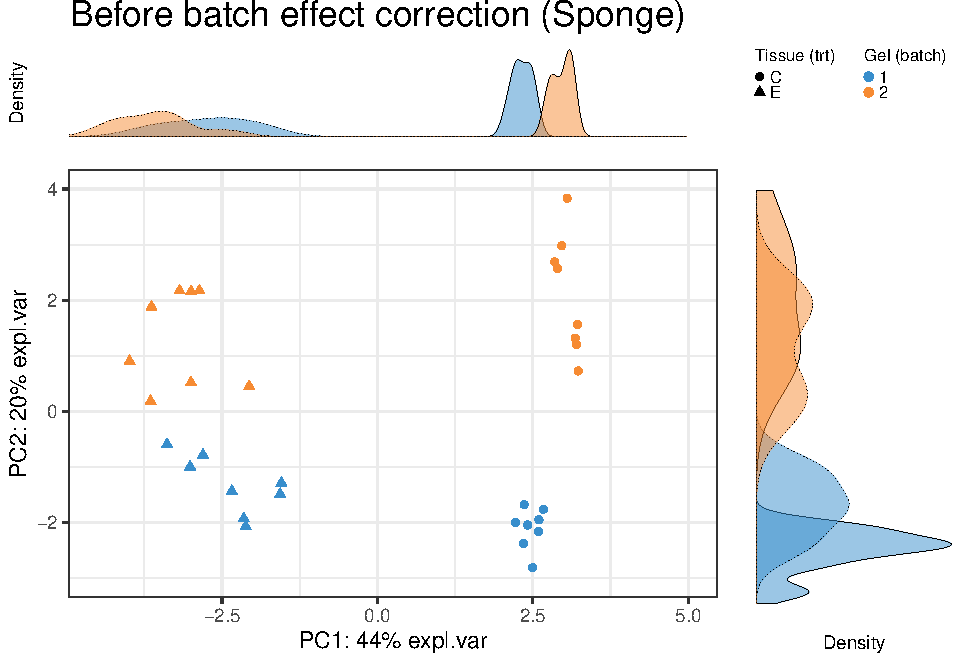
\includegraphics{Managing_batch_effects_files/figure-latex/unnamed-chunk-7-1.pdf}

In sponge data, the first PC (explaining the largest source of
variation) shows variation between samples from different tissues (the
effect of interest), while the second PC (explaining the second largest
source of variation) displays sample differences due to different
batches, as also highlighted in the density plots per component.
Therefore, PCA plots can inform not only of the presence of batch
effects, but also which variation is the largest in the data. In this
particular dataset, the effect of interest variation is larger than
batch variation.

\begin{Shaded}
\begin{Highlighting}[]
\CommentTok{# ad data}
\KeywordTok{Scatter_Density}\NormalTok{(}\DataTypeTok{data =}\NormalTok{ ad.pca.before}\OperatorTok{$}\NormalTok{variates}\OperatorTok{$}\NormalTok{X, }\DataTypeTok{batch =}\NormalTok{ ad.batch, }
                \DataTypeTok{trt =}\NormalTok{ ad.trt, }\DataTypeTok{expl.var =}\NormalTok{ ad.pca.before}\OperatorTok{$}\NormalTok{explained_variance, }
                \DataTypeTok{xlim =} \KeywordTok{c}\NormalTok{(}\OperatorTok{-}\DecValTok{15}\NormalTok{,}\DecValTok{14}\NormalTok{), }\DataTypeTok{ylim =} \KeywordTok{c}\NormalTok{(}\OperatorTok{-}\DecValTok{13}\NormalTok{,}\DecValTok{14}\NormalTok{), }
                \DataTypeTok{batch.legend.title =} \StringTok{'Date (batch)'}\NormalTok{, }
                \DataTypeTok{trt.legend.title =} \StringTok{'Conc (trt)'}\NormalTok{, }
                \DataTypeTok{title =} \StringTok{'Before batch effect correction (AD)'}\NormalTok{)}
\end{Highlighting}
\end{Shaded}

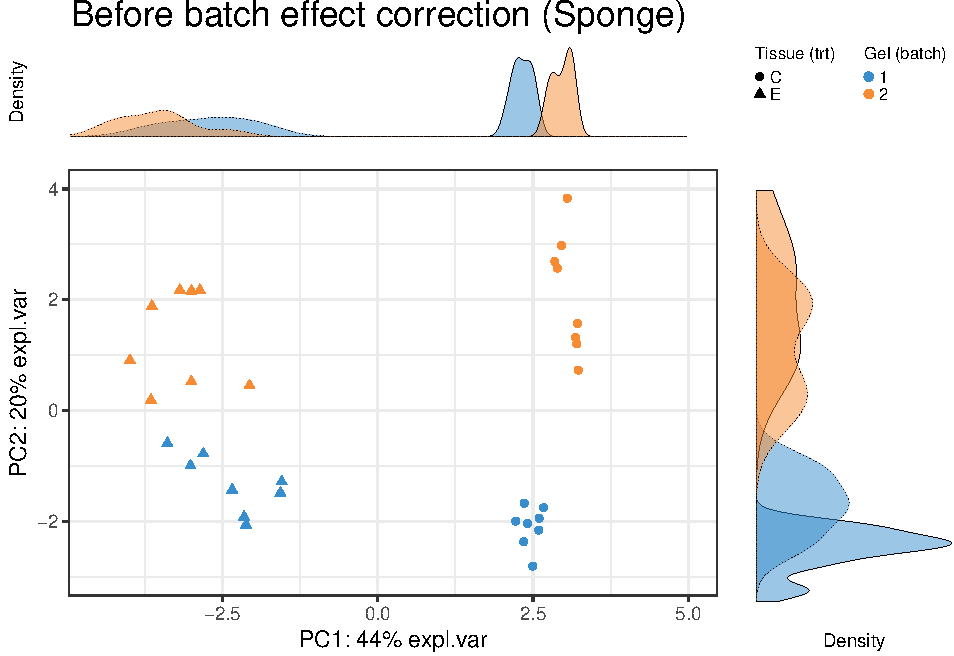
\includegraphics{Managing_batch_effects_files/figure-latex/unnamed-chunk-8-1.pdf}

In AD data, we observe a separation of samples from batch 14/04/2016.
The batch variation is mostly explained by the second PC.

\begin{Shaded}
\begin{Highlighting}[]
\CommentTok{# hd data}
\KeywordTok{Scatter_Density}\NormalTok{(}\DataTypeTok{data =}\NormalTok{ hd.pca.before}\OperatorTok{$}\NormalTok{variates}\OperatorTok{$}\NormalTok{X, }\DataTypeTok{batch =}\NormalTok{ hd.batch, }
                \DataTypeTok{trt =}\NormalTok{ hd.trt, }\DataTypeTok{expl.var =}\NormalTok{ hd.pca.before}\OperatorTok{$}\NormalTok{explained_variance, }
                \DataTypeTok{xlim =} \KeywordTok{c}\NormalTok{(}\OperatorTok{-}\DecValTok{20}\NormalTok{,}\DecValTok{20}\NormalTok{), }\DataTypeTok{ylim =} \KeywordTok{c}\NormalTok{(}\OperatorTok{-}\DecValTok{25}\NormalTok{,}\DecValTok{15}\NormalTok{), }
                \DataTypeTok{batch.legend.title =} \StringTok{'Cage (batch)'}\NormalTok{, }
                \DataTypeTok{trt.legend.title =} \StringTok{'Genotype (trt)'}\NormalTok{, }
                \DataTypeTok{title =} \StringTok{'Before batch effect correction (HD)'}\NormalTok{)}
\end{Highlighting}
\end{Shaded}

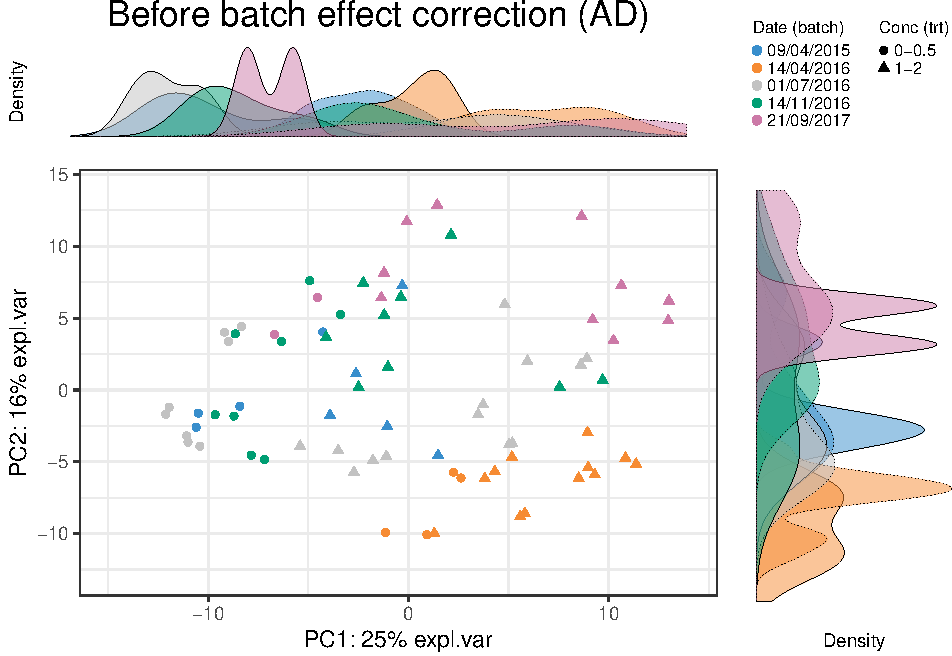
\includegraphics{Managing_batch_effects_files/figure-latex/unnamed-chunk-9-1.pdf}

In HD data, batch effect is due to different cages and obvious. The
batch variation is both explained by the first and second PC.

\section{Density plot and box plot}\label{density-plot-and-box-plot}

For non systematic batch effects, it is useful to visualise a few OTUs
individually. We apply density plots and box plots on OTUs, one at a
time from each dataset to visualise batch effects. But only one OTU each
dataset is selected as examples.

We randomly select OTU9 in sponge data, and generate density plots and
box plots separately across samples within each batch to observe whether
batch effects serve as a major source of variation.

\begin{Shaded}
\begin{Highlighting}[]
\CommentTok{# sponge data}
\NormalTok{sponge.before.df <-}\StringTok{ }\KeywordTok{data.frame}\NormalTok{(}\DataTypeTok{value =}\NormalTok{ sponge.tss.clr[,}\DecValTok{9}\NormalTok{], }\DataTypeTok{batch =}\NormalTok{ sponge.batch)}

\KeywordTok{box_plot_fun}\NormalTok{(}\DataTypeTok{data =}\NormalTok{ sponge.before.df, }\DataTypeTok{x =}\NormalTok{ sponge.before.df}\OperatorTok{$}\NormalTok{batch,}
             \DataTypeTok{y =}\NormalTok{ sponge.before.df}\OperatorTok{$}\NormalTok{value, }\DataTypeTok{title =} \StringTok{'OTU9 (Sponge)'}\NormalTok{,}
             \DataTypeTok{batch.legend.title =} \StringTok{'Gel (batch)'}\NormalTok{)}
\end{Highlighting}
\end{Shaded}

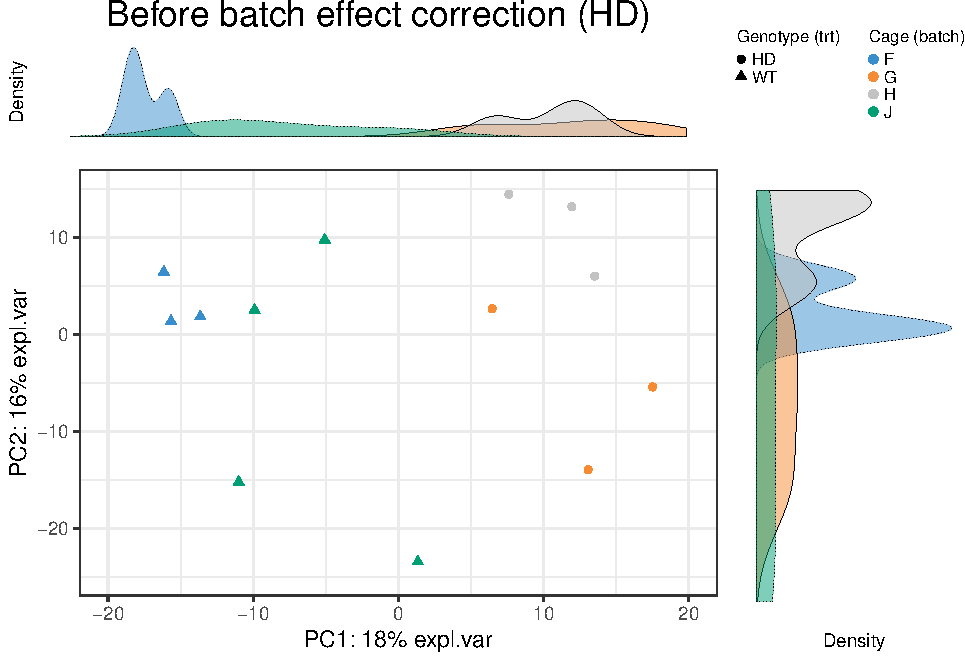
\includegraphics{Managing_batch_effects_files/figure-latex/unnamed-chunk-10-1.pdf}

\begin{Shaded}
\begin{Highlighting}[]
\KeywordTok{ggplot}\NormalTok{(sponge.before.df, }\KeywordTok{aes}\NormalTok{(}\DataTypeTok{x =}\NormalTok{ value, }\DataTypeTok{fill =}\NormalTok{ batch)) }\OperatorTok{+}\StringTok{ }
\StringTok{  }\KeywordTok{geom_density}\NormalTok{(}\DataTypeTok{alpha =} \FloatTok{0.5}\NormalTok{) }\OperatorTok{+}\StringTok{ }\KeywordTok{scale_fill_manual}\NormalTok{(}\DataTypeTok{values =} \KeywordTok{color.mixo}\NormalTok{(}\DecValTok{1}\OperatorTok{:}\DecValTok{10}\NormalTok{)) }\OperatorTok{+}\StringTok{ }
\StringTok{  }\KeywordTok{labs}\NormalTok{(}\DataTypeTok{title =} \StringTok{'OTU9 (Sponge)'}\NormalTok{, }\DataTypeTok{x =} \StringTok{'Value'}\NormalTok{, }\DataTypeTok{fill =} \StringTok{'Gel (batch)'}\NormalTok{) }\OperatorTok{+}\StringTok{ }
\StringTok{  }\KeywordTok{theme_bw}\NormalTok{() }\OperatorTok{+}\StringTok{ }\KeywordTok{theme}\NormalTok{(}\DataTypeTok{plot.title =} \KeywordTok{element_text}\NormalTok{(}\DataTypeTok{hjust =} \FloatTok{0.5}\NormalTok{), }
                     \DataTypeTok{panel.grid =} \KeywordTok{element_blank}\NormalTok{())}
\end{Highlighting}
\end{Shaded}

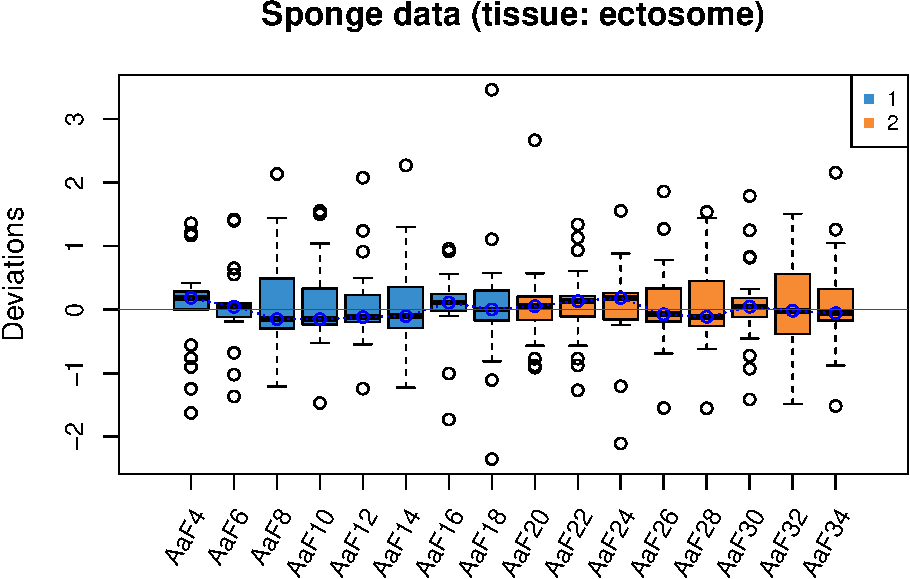
\includegraphics{Managing_batch_effects_files/figure-latex/unnamed-chunk-10-2.pdf}

For the proportional abundance of OTU9, the samples within different
batches are very distinct, indicating a strong batch effect in sponge
data.

Assuming the data fit the distribution of the linear model (which is the
case here after CLR transformation), we can also assess the effect of
batch in a linear model on that particular OTU9:

\begin{Shaded}
\begin{Highlighting}[]
\NormalTok{sponge.lm <-}\StringTok{ }\KeywordTok{lm}\NormalTok{(sponge.tss.clr[,}\DecValTok{9}\NormalTok{] }\OperatorTok{~}\StringTok{ }\NormalTok{sponge.trt }\OperatorTok{+}\StringTok{ }\NormalTok{sponge.batch)}
\KeywordTok{summary}\NormalTok{(sponge.lm)}
\end{Highlighting}
\end{Shaded}

\begin{verbatim}
## 
## Call:
## lm(formula = sponge.tss.clr[, 9] ~ sponge.trt + sponge.batch)
## 
## Residuals:
##      Min       1Q   Median       3Q      Max 
## -1.87967 -0.24705  0.04588  0.24492  1.00757 
## 
## Coefficients:
##               Estimate Std. Error t value Pr(>|t|)    
## (Intercept)     1.7849     0.1497  11.922 1.06e-12 ***
## sponge.trtE     0.1065     0.1729   0.616    0.543    
## sponge.batch2  -0.7910     0.1729  -4.575 8.24e-05 ***
## ---
## Signif. codes:  0 '***' 0.001 '**' 0.01 '*' 0.05 '.' 0.1 ' ' 1
## 
## Residual standard error: 0.489 on 29 degrees of freedom
## Multiple R-squared:  0.4236, Adjusted R-squared:  0.3839 
## F-statistic: 10.66 on 2 and 29 DF,  p-value: 0.0003391
\end{verbatim}

The batch (gel) effect is statistically significant (P \(<\) 0.001), as
indicated in the \textbf{sponge.batch2} row.

\begin{Shaded}
\begin{Highlighting}[]
\CommentTok{# ad data}
\NormalTok{ad.before.df <-}\StringTok{ }\KeywordTok{data.frame}\NormalTok{(}\DataTypeTok{value =}\NormalTok{ ad.clr[,}\DecValTok{1}\NormalTok{], }\DataTypeTok{batch =}\NormalTok{ ad.batch)}

\KeywordTok{box_plot_fun}\NormalTok{(}\DataTypeTok{data =}\NormalTok{ ad.before.df,}\DataTypeTok{x =}\NormalTok{ ad.before.df}\OperatorTok{$}\NormalTok{batch,}
             \DataTypeTok{y =}\NormalTok{ ad.before.df}\OperatorTok{$}\NormalTok{value, }\DataTypeTok{title =} \StringTok{'OTU12 (AD)'}\NormalTok{,}
             \DataTypeTok{batch.legend.title =} \StringTok{'Date (batch)'}\NormalTok{,}
             \DataTypeTok{x.angle =} \DecValTok{45}\NormalTok{, }\DataTypeTok{x.hjust =} \DecValTok{1}\NormalTok{)}
\end{Highlighting}
\end{Shaded}

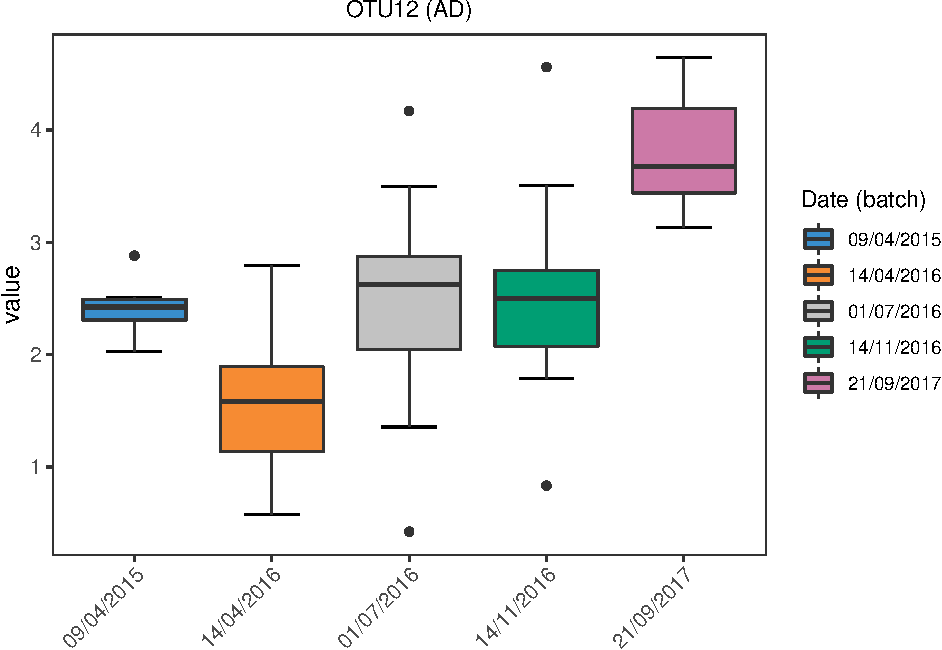
\includegraphics{Managing_batch_effects_files/figure-latex/unnamed-chunk-12-1.pdf}

\begin{Shaded}
\begin{Highlighting}[]
\KeywordTok{ggplot}\NormalTok{(ad.before.df, }\KeywordTok{aes}\NormalTok{(}\DataTypeTok{x =}\NormalTok{ value, }\DataTypeTok{fill =}\NormalTok{ batch)) }\OperatorTok{+}\StringTok{ }
\StringTok{  }\KeywordTok{geom_density}\NormalTok{(}\DataTypeTok{alpha =} \FloatTok{0.5}\NormalTok{) }\OperatorTok{+}\StringTok{ }\KeywordTok{scale_fill_manual}\NormalTok{(}\DataTypeTok{values =} \KeywordTok{color.mixo}\NormalTok{(}\DecValTok{1}\OperatorTok{:}\DecValTok{10}\NormalTok{)) }\OperatorTok{+}\StringTok{ }
\StringTok{  }\KeywordTok{labs}\NormalTok{(}\DataTypeTok{title =} \StringTok{'OTU12 (AD)'}\NormalTok{,}\DataTypeTok{x =} \StringTok{'Value'}\NormalTok{,}\DataTypeTok{fill =} \StringTok{'Date (batch)'}\NormalTok{) }\OperatorTok{+}\StringTok{ }
\StringTok{  }\KeywordTok{theme_bw}\NormalTok{() }\OperatorTok{+}\StringTok{ }\KeywordTok{theme}\NormalTok{(}\DataTypeTok{plot.title =} \KeywordTok{element_text}\NormalTok{(}\DataTypeTok{hjust =} \FloatTok{0.5}\NormalTok{), }
                     \DataTypeTok{panel.grid =} \KeywordTok{element_blank}\NormalTok{())}
\end{Highlighting}
\end{Shaded}

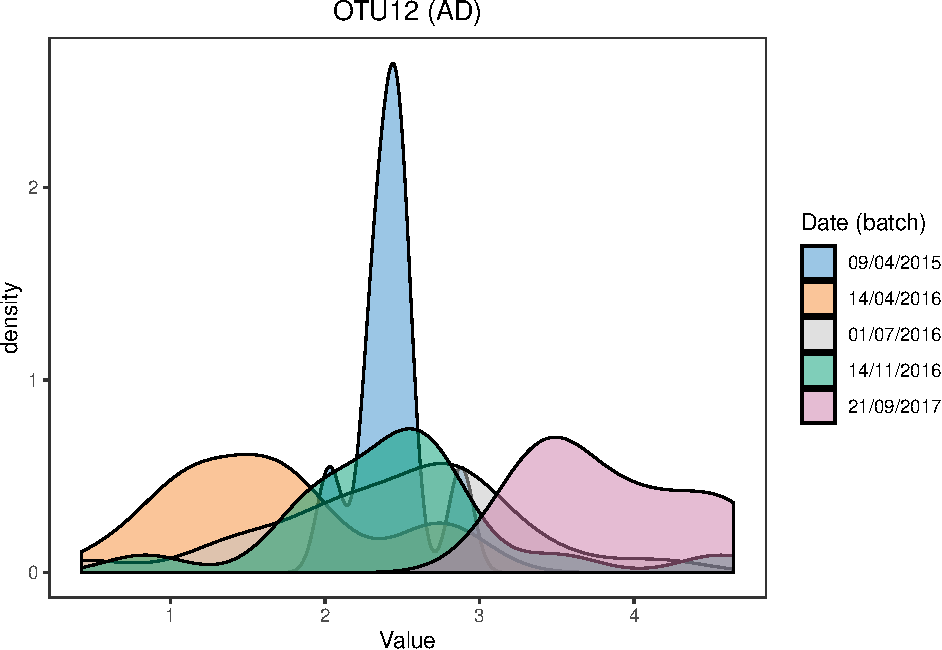
\includegraphics{Managing_batch_effects_files/figure-latex/unnamed-chunk-12-2.pdf}

Batch effects in AD data are also easily visualised.

\begin{Shaded}
\begin{Highlighting}[]
\NormalTok{ad.lm <-}\StringTok{ }\KeywordTok{lm}\NormalTok{(ad.clr[,}\DecValTok{1}\NormalTok{] }\OperatorTok{~}\StringTok{ }\NormalTok{ad.trt }\OperatorTok{+}\StringTok{ }\NormalTok{ad.batch)}
\KeywordTok{anova}\NormalTok{(ad.lm)}
\end{Highlighting}
\end{Shaded}

\begin{verbatim}
## Analysis of Variance Table
## 
## Response: ad.clr[, 1]
##           Df Sum Sq Mean Sq F value    Pr(>F)    
## ad.trt     1  1.460  1.4605  3.1001   0.08272 .  
## ad.batch   4 32.889  8.2222 17.4532 6.168e-10 ***
## Residuals 69 32.506  0.4711                      
## ---
## Signif. codes:  0 '***' 0.001 '**' 0.01 '*' 0.05 '.' 0.1 ' ' 1
\end{verbatim}

In AD data, the difference between batches (dates) is statistically
significant (P \textless{} 0.001, as tested with ANOVA). We can also
obtain P values between each two batch categories.

\begin{Shaded}
\begin{Highlighting}[]
\KeywordTok{summary}\NormalTok{(ad.lm)}
\end{Highlighting}
\end{Shaded}

\begin{verbatim}
## 
## Call:
## lm(formula = ad.clr[, 1] ~ ad.trt + ad.batch)
## 
## Residuals:
##      Min       1Q   Median       3Q      Max 
## -2.09885 -0.39613 -0.00381  0.36645  1.98185 
## 
## Coefficients:
##                     Estimate Std. Error t value Pr(>|t|)    
## (Intercept)         2.311213   0.247768   9.328 7.57e-14 ***
## ad.trt1-2           0.203619   0.171183   1.189  0.23833    
## ad.batch14/04/2016 -0.828100   0.287918  -2.876  0.00535 ** 
## ad.batch01/07/2016  0.007239   0.273672   0.026  0.97897    
## ad.batch14/11/2016  0.062689   0.282978   0.222  0.82533    
## ad.batch21/09/2017  1.361132   0.306373   4.443 3.30e-05 ***
## ---
## Signif. codes:  0 '***' 0.001 '**' 0.01 '*' 0.05 '.' 0.1 ' ' 1
## 
## Residual standard error: 0.6864 on 69 degrees of freedom
## Multiple R-squared:  0.5138, Adjusted R-squared:  0.4786 
## F-statistic: 14.58 on 5 and 69 DF,  p-value: 9.665e-10
\end{verbatim}

\begin{Shaded}
\begin{Highlighting}[]
\CommentTok{# hd data}
\NormalTok{hd.before.df <-}\StringTok{ }\KeywordTok{data.frame}\NormalTok{(}\DataTypeTok{value =}\NormalTok{ hd.clr[,}\DecValTok{1}\NormalTok{], }\DataTypeTok{batch =}\NormalTok{ hd.batch)}

\KeywordTok{box_plot_fun}\NormalTok{(}\DataTypeTok{data =}\NormalTok{ hd.before.df, }\DataTypeTok{x =}\NormalTok{ hd.before.df}\OperatorTok{$}\NormalTok{batch,}
             \DataTypeTok{y =}\NormalTok{ hd.before.df}\OperatorTok{$}\NormalTok{value,}\DataTypeTok{title =} \StringTok{'OTU1 (HD)'}\NormalTok{,}
             \DataTypeTok{batch.legend.title =} \StringTok{'Cage (batch)'}\NormalTok{)}
\end{Highlighting}
\end{Shaded}

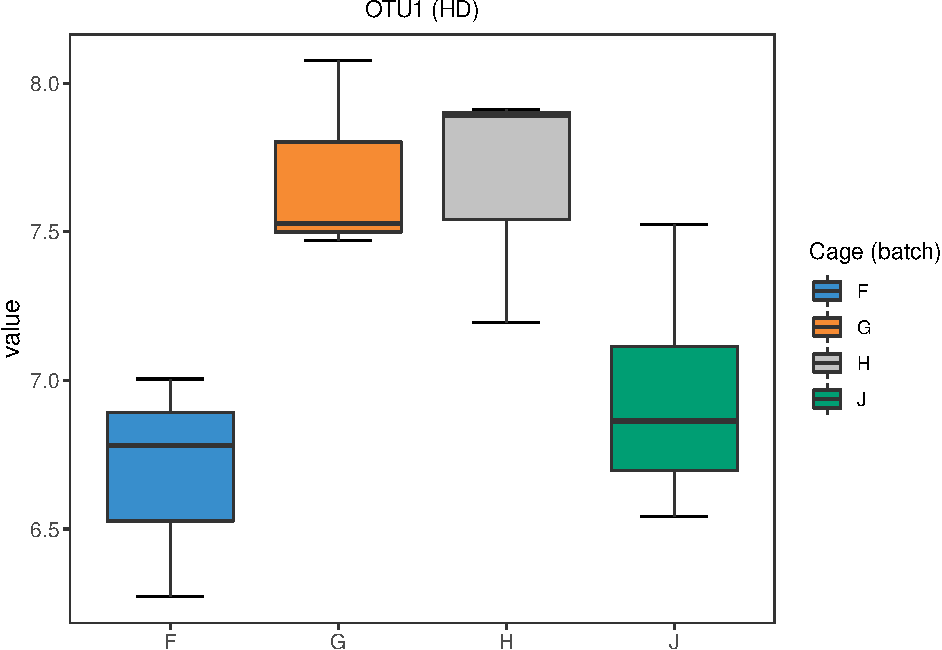
\includegraphics{Managing_batch_effects_files/figure-latex/unnamed-chunk-15-1.pdf}

\begin{Shaded}
\begin{Highlighting}[]
\KeywordTok{ggplot}\NormalTok{(hd.before.df, }\KeywordTok{aes}\NormalTok{(}\DataTypeTok{x =}\NormalTok{ value, }\DataTypeTok{fill =}\NormalTok{ batch)) }\OperatorTok{+}\StringTok{ }
\StringTok{  }\KeywordTok{geom_density}\NormalTok{(}\DataTypeTok{alpha =} \FloatTok{0.5}\NormalTok{) }\OperatorTok{+}\StringTok{ }\KeywordTok{scale_fill_manual}\NormalTok{(}\DataTypeTok{values =} \KeywordTok{color.mixo}\NormalTok{(}\DecValTok{1}\OperatorTok{:}\DecValTok{10}\NormalTok{)) }\OperatorTok{+}\StringTok{ }
\StringTok{  }\KeywordTok{labs}\NormalTok{(}\DataTypeTok{title =} \StringTok{'OTU1 (HD)'}\NormalTok{,}\DataTypeTok{x =} \StringTok{'Value'}\NormalTok{,}\DataTypeTok{fill =} \StringTok{'Cage (batch)'}\NormalTok{) }\OperatorTok{+}\StringTok{ }
\StringTok{  }\KeywordTok{theme_bw}\NormalTok{() }\OperatorTok{+}\StringTok{ }\KeywordTok{theme}\NormalTok{(}\DataTypeTok{plot.title =} \KeywordTok{element_text}\NormalTok{(}\DataTypeTok{hjust =} \FloatTok{0.5}\NormalTok{), }
                     \DataTypeTok{panel.grid =} \KeywordTok{element_blank}\NormalTok{())}
\end{Highlighting}
\end{Shaded}

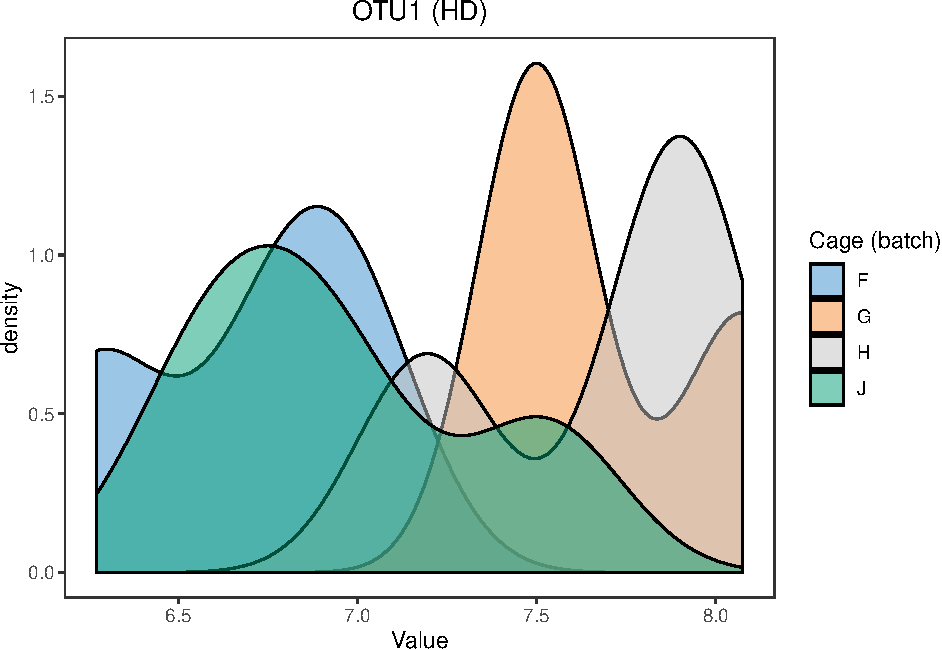
\includegraphics{Managing_batch_effects_files/figure-latex/unnamed-chunk-15-2.pdf}

In HD data, we easily detect the differences between samples within
different batches.

\begin{Shaded}
\begin{Highlighting}[]
\NormalTok{hd.lm <-}\StringTok{ }\KeywordTok{lm}\NormalTok{(hd.clr[,}\DecValTok{1}\NormalTok{] }\OperatorTok{~}\StringTok{ }\NormalTok{hd.batch)}
\KeywordTok{anova}\NormalTok{(hd.lm)}
\end{Highlighting}
\end{Shaded}

\begin{verbatim}
## Analysis of Variance Table
## 
## Response: hd.clr[, 1]
##           Df Sum Sq Mean Sq F value  Pr(>F)  
## hd.batch   3 2.4108 0.80359  5.2569 0.02276 *
## Residuals  9 1.3758 0.15286                  
## ---
## Signif. codes:  0 '***' 0.001 '**' 0.01 '*' 0.05 '.' 0.1 ' ' 1
\end{verbatim}

As the batch x treatment design of HD data is nested and unbalanced, the
linear model with both treatment (genotype) and batch (cage) is unable
to fit. We therefore fit a linear model with batch effect only. The
difference between cages is statistically significant (P \textless{}
0.05). But the difference may also be influenced by treatment and we are
unable to exclude treatment influence.

\section{RLE plots}\label{rle-plots}

RLE plots can be plotted using `RleMicroRna' in R package `AgiMicroRna'.
Here, we made some changes on the function `RleMicroRna', called
`RleMicroRna2' and available on our extra functions `Functions.R'.

RLE plots are based on the assumption that the majority of microbial
variables are unaffected by the effect of interest, and therefore any
sample heterogeneity observed - i.e.~different distributions and their
variances, and medians different from zero, should indicate the presence
of batch effects. In our case studies, the treatment information is
known, so we generate multiple RLE plots per treatment group, as
suggested by \citep{lin2018scmerge}.

In sponge data, we group the samples according to the tissue (choanosome
/ ectosome) and generate two RLE plots:

\begin{Shaded}
\begin{Highlighting}[]
\CommentTok{# sponge data}
\NormalTok{sponge.batch_c <-}\StringTok{ }\NormalTok{sponge.batch[sponge.trt }\OperatorTok{==}\StringTok{ 'C'}\NormalTok{]}
\NormalTok{sponge.batch_e <-}\StringTok{ }\NormalTok{sponge.batch[sponge.trt }\OperatorTok{==}\StringTok{ 'E'}\NormalTok{] }

\NormalTok{sponge.before_c <-}\StringTok{ }\NormalTok{sponge.tss.clr[sponge.trt }\OperatorTok{==}\StringTok{ 'C'}\NormalTok{, ]}
\NormalTok{sponge.before_e <-}\StringTok{ }\NormalTok{sponge.tss.clr[sponge.trt }\OperatorTok{==}\StringTok{ 'E'}\NormalTok{, ] }


\KeywordTok{RleMicroRna2}\NormalTok{(}\DataTypeTok{object =} \KeywordTok{t}\NormalTok{(sponge.before_c), }\DataTypeTok{batch =}\NormalTok{ sponge.batch_c, }
             \DataTypeTok{maintitle =} \StringTok{'Sponge (tissue: choanosome)'}\NormalTok{)}
\end{Highlighting}
\end{Shaded}

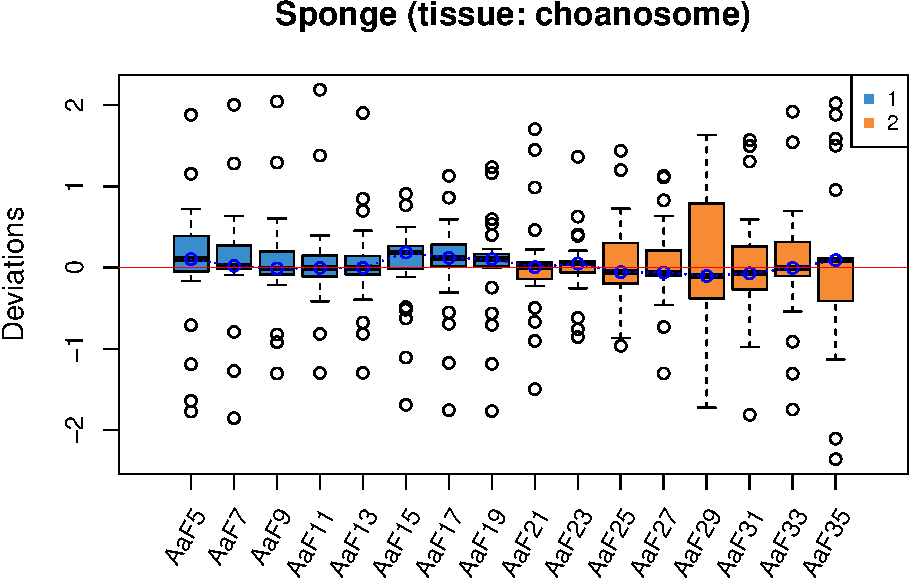
\includegraphics{Managing_batch_effects_files/figure-latex/unnamed-chunk-17-1.pdf}

\begin{Shaded}
\begin{Highlighting}[]
\KeywordTok{RleMicroRna2}\NormalTok{(}\DataTypeTok{object =} \KeywordTok{t}\NormalTok{(sponge.before_e), }\DataTypeTok{batch =}\NormalTok{ sponge.batch_e, }
             \DataTypeTok{maintitle =} \StringTok{'Sponge (tissue: ectosome)'}\NormalTok{)}
\end{Highlighting}
\end{Shaded}

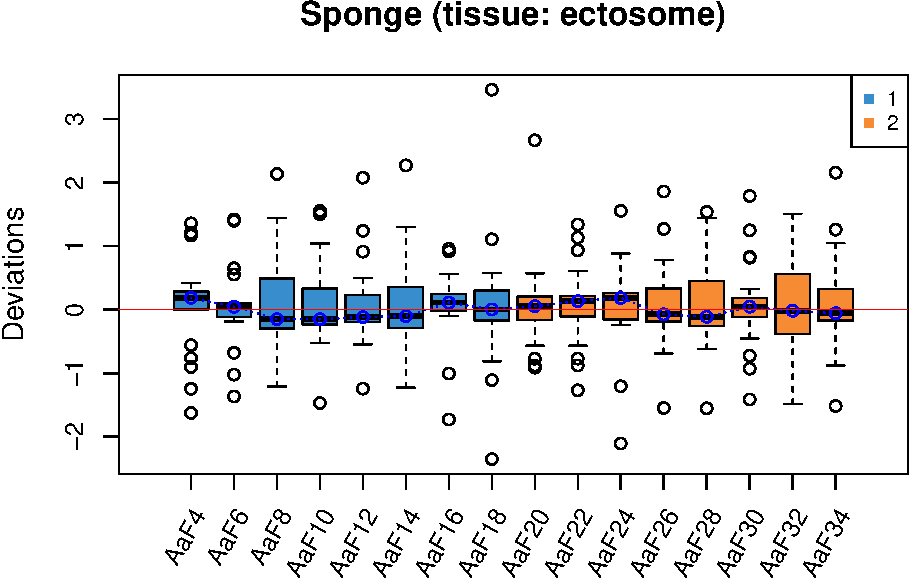
\includegraphics{Managing_batch_effects_files/figure-latex/unnamed-chunk-17-2.pdf}

For both RLE plots with samples from different tissues, the batch effect
is not obvious as all medians of samples are close to zero, but Gel2 has
a greater interquartile range (IQR) than the other samples.

\begin{Shaded}
\begin{Highlighting}[]
\CommentTok{# ad data}
\NormalTok{ad.batch_}\DecValTok{05}\NormalTok{ <-}\StringTok{ }\NormalTok{ad.batch[ad.trt }\OperatorTok{==}\StringTok{ '0-0.5'}\NormalTok{]}
\NormalTok{ad.batch_}\DecValTok{2}\NormalTok{ <-}\StringTok{ }\NormalTok{ad.batch[ad.trt }\OperatorTok{==}\StringTok{ '1-2'}\NormalTok{] }

\NormalTok{ad.before_}\DecValTok{05}\NormalTok{ <-}\StringTok{ }\NormalTok{ad.clr[ad.trt }\OperatorTok{==}\StringTok{ '0-0.5'}\NormalTok{, ]}
\NormalTok{ad.before_}\DecValTok{2}\NormalTok{ <-}\StringTok{ }\NormalTok{ad.clr[ad.trt }\OperatorTok{==}\StringTok{ '1-2'}\NormalTok{, ]}

\KeywordTok{RleMicroRna2}\NormalTok{(}\DataTypeTok{object =} \KeywordTok{t}\NormalTok{(ad.before_}\DecValTok{05}\NormalTok{), }\DataTypeTok{batch =}\NormalTok{ ad.batch_}\DecValTok{05}\NormalTok{, }
             \DataTypeTok{maintitle =} \StringTok{'AD (initial phenol conc: 0-0.5 g/L)'}\NormalTok{, }
             \DataTypeTok{legend.cex =} \FloatTok{0.5}\NormalTok{)}
\end{Highlighting}
\end{Shaded}

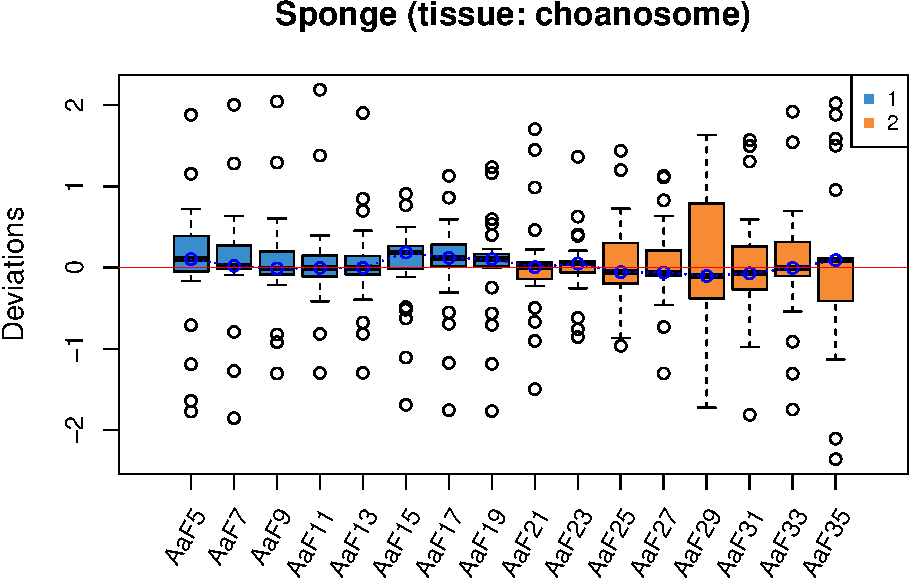
\includegraphics{Managing_batch_effects_files/figure-latex/unnamed-chunk-18-1.pdf}

\begin{Shaded}
\begin{Highlighting}[]
\KeywordTok{RleMicroRna2}\NormalTok{(}\DataTypeTok{object =} \KeywordTok{t}\NormalTok{(ad.before_}\DecValTok{2}\NormalTok{), }\DataTypeTok{batch =}\NormalTok{ ad.batch_}\DecValTok{2}\NormalTok{, }
             \DataTypeTok{maintitle =} \StringTok{'AD (initial phenol conc: 1-2 g/L)'}\NormalTok{, }
             \DataTypeTok{cex.xaxis =} \FloatTok{0.7}\NormalTok{, }\DataTypeTok{legend.cex =} \FloatTok{0.5}\NormalTok{)}
\end{Highlighting}
\end{Shaded}

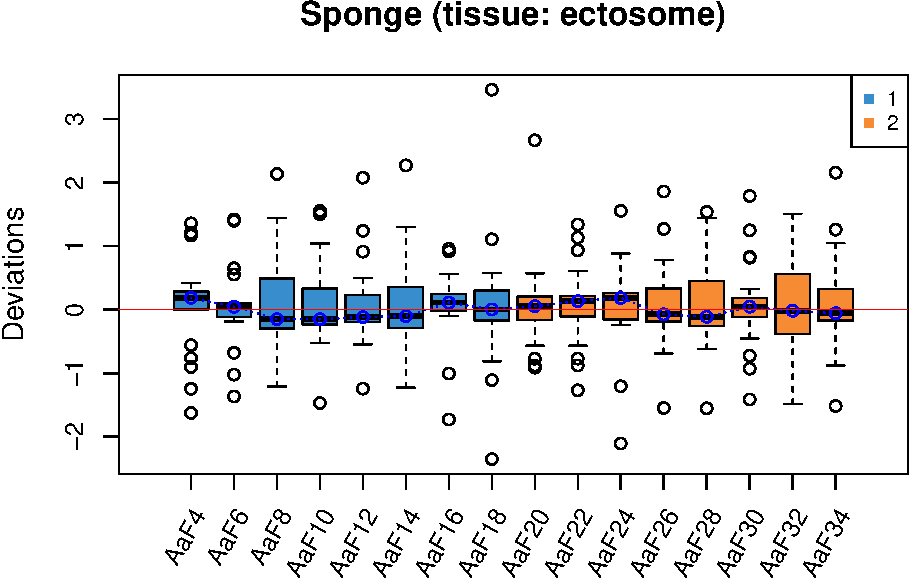
\includegraphics{Managing_batch_effects_files/figure-latex/unnamed-chunk-18-2.pdf}

In RLE plots for the AD data, the batch effect is also not obvious as
all medians of samples are close to zero, but the samples dated
14/04/2016 may be affected by batch as they have a greater IQR than the
other samples.

\begin{Shaded}
\begin{Highlighting}[]
\CommentTok{# hd data}
\NormalTok{hd.batch_h <-}\StringTok{ }\NormalTok{hd.batch[hd.trt }\OperatorTok{==}\StringTok{ 'HD'}\NormalTok{]}
\NormalTok{hd.batch_w <-}\StringTok{ }\NormalTok{hd.batch[hd.trt }\OperatorTok{==}\StringTok{ 'WT'}\NormalTok{] }

\NormalTok{hd.before_h <-}\StringTok{ }\NormalTok{hd.clr[hd.trt }\OperatorTok{==}\StringTok{ 'HD'}\NormalTok{, ]}
\NormalTok{hd.before_w <-}\StringTok{ }\NormalTok{hd.clr[hd.trt }\OperatorTok{==}\StringTok{ 'WT'}\NormalTok{, ]}

\KeywordTok{RleMicroRna2}\NormalTok{(}\DataTypeTok{object =} \KeywordTok{t}\NormalTok{(hd.before_h), }\DataTypeTok{batch =}\NormalTok{ hd.batch_h, }
             \DataTypeTok{maintitle =} \StringTok{'HD (genotype: HD)'}\NormalTok{)}
\end{Highlighting}
\end{Shaded}

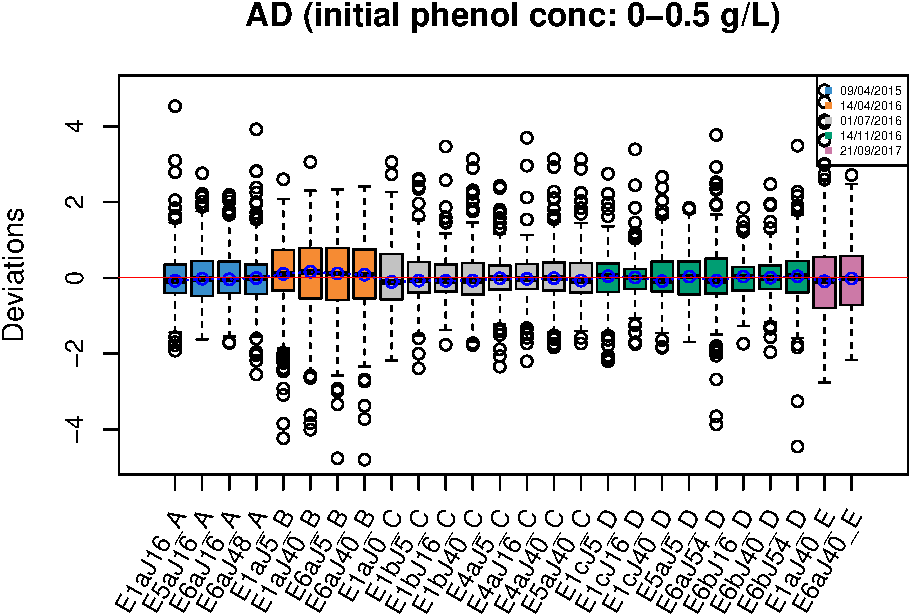
\includegraphics{Managing_batch_effects_files/figure-latex/unnamed-chunk-19-1.pdf}

\begin{Shaded}
\begin{Highlighting}[]
\KeywordTok{RleMicroRna2}\NormalTok{(}\DataTypeTok{object =} \KeywordTok{t}\NormalTok{(hd.before_w), }\DataTypeTok{batch =}\NormalTok{ hd.batch_w, }
             \DataTypeTok{maintitle =} \StringTok{'HD (genotype: WT)'}\NormalTok{)}
\end{Highlighting}
\end{Shaded}

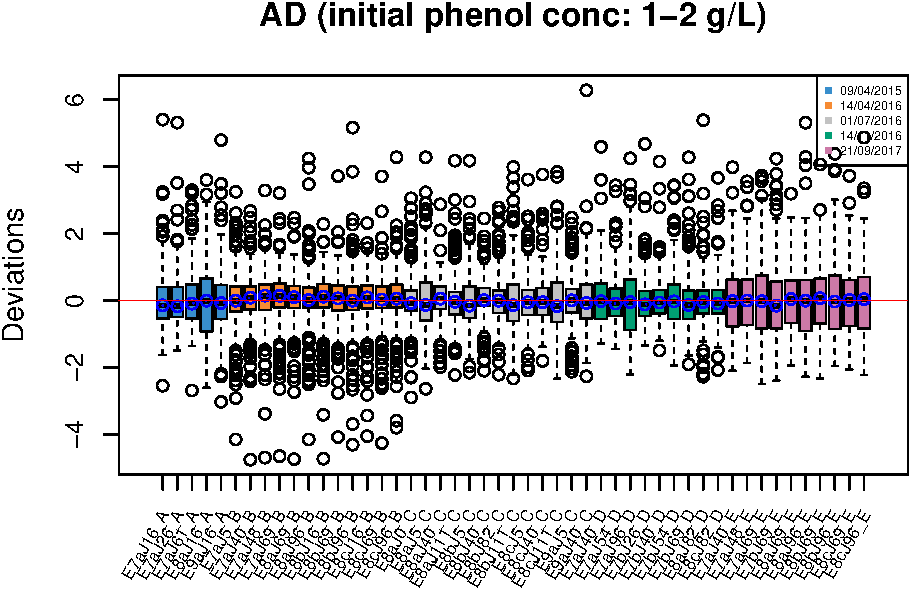
\includegraphics{Managing_batch_effects_files/figure-latex/unnamed-chunk-19-2.pdf}

The batch effect in HD data is not easily detected, but Cage G has a
greater IQR than the other samples, which may indicate a batch effect.

\section{Heatmap}\label{heatmap}

Clustering analysis can be used to detect batch effects. Ideally samples
with the same treatment will be clustered together, data clustered by
batches instead of treatments indicate a batch effect. Heatmaps and
dendrograms are two common approaches to visualise the clusters.

\begin{Shaded}
\begin{Highlighting}[]
\CommentTok{# Sponge data}
\CommentTok{# scale on OTUs}
\NormalTok{sponge.tss.clr.scale <-}\StringTok{ }\KeywordTok{scale}\NormalTok{(sponge.tss.clr, }\DataTypeTok{center =}\NormalTok{ T, }\DataTypeTok{scale =}\NormalTok{ T) }
\CommentTok{# scale on samples}
\NormalTok{sponge.tss.clr.scale <-}\StringTok{ }\KeywordTok{scale}\NormalTok{(}\KeywordTok{t}\NormalTok{(sponge.tss.clr.scale), }\DataTypeTok{center =}\NormalTok{ T, }\DataTypeTok{scale =}\NormalTok{ T) }

\NormalTok{sponge.anno_col <-}\StringTok{ }\KeywordTok{data.frame}\NormalTok{(}\DataTypeTok{Batch =}\NormalTok{ sponge.batch, }\DataTypeTok{Tissue =}\NormalTok{ sponge.trt)}
\NormalTok{sponge.anno_metabo_colors <-}\StringTok{ }\KeywordTok{list}\NormalTok{(}\DataTypeTok{Batch =} \KeywordTok{c}\NormalTok{(}\StringTok{'1'}\NormalTok{ =}\StringTok{ '#388ECC'}\NormalTok{, }\StringTok{'2'}\NormalTok{ =}\StringTok{ '#F68B33'}\NormalTok{), }
                                 \DataTypeTok{Tissue =} \KeywordTok{c}\NormalTok{(}\DataTypeTok{C =} \StringTok{'#F0E442'}\NormalTok{, }\DataTypeTok{E =} \StringTok{'#D55E00'}\NormalTok{))}


\KeywordTok{pheatmap}\NormalTok{(sponge.tss.clr.scale, }
         \DataTypeTok{scale =} \StringTok{'none'}\NormalTok{, }
         \DataTypeTok{cluster_rows =}\NormalTok{ F, }
         \DataTypeTok{cluster_cols =}\NormalTok{ T, }
         \DataTypeTok{fontsize_row =} \DecValTok{5}\NormalTok{, }\DataTypeTok{fontsize_col =} \DecValTok{8}\NormalTok{,}
         \DataTypeTok{fontsize =} \DecValTok{8}\NormalTok{,}
         \DataTypeTok{clustering_distance_rows =} \StringTok{'euclidean'}\NormalTok{,}
         \DataTypeTok{clustering_method =} \StringTok{'ward.D'}\NormalTok{,}
         \DataTypeTok{treeheight_row =} \DecValTok{30}\NormalTok{,}
         \DataTypeTok{annotation_col =}\NormalTok{ sponge.anno_col,}
         \DataTypeTok{annotation_colors =}\NormalTok{ sponge.anno_metabo_colors,}
         \DataTypeTok{border_color =} \StringTok{'NA'}\NormalTok{,}
         \DataTypeTok{main =} \StringTok{'Sponge data - Scaled'}\NormalTok{)}
\end{Highlighting}
\end{Shaded}

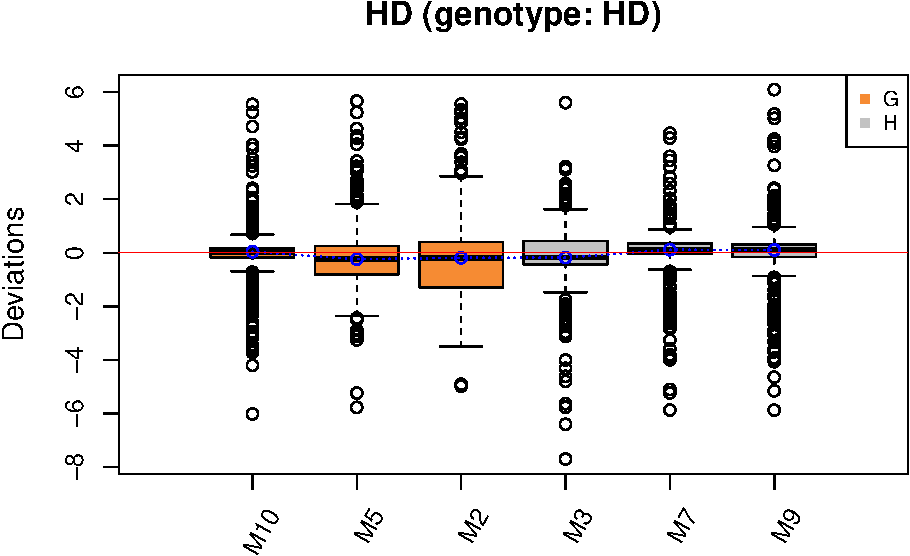
\includegraphics{Managing_batch_effects_files/figure-latex/unnamed-chunk-20-1.pdf}

In sponge data, samples are preferentially clustered by batch instead of
tissue type, indicating a batch effect.

\begin{Shaded}
\begin{Highlighting}[]
\CommentTok{# AD data}
\NormalTok{ad.clr.scale <-}\StringTok{ }\KeywordTok{scale}\NormalTok{(ad.clr,}\DataTypeTok{center =}\NormalTok{ T, }\DataTypeTok{scale =}\NormalTok{ T)}
\NormalTok{ad.clr.scale <-}\StringTok{ }\KeywordTok{scale}\NormalTok{(}\KeywordTok{t}\NormalTok{(ad.clr.scale), }\DataTypeTok{center =}\NormalTok{ T, }\DataTypeTok{scale =}\NormalTok{ T)}

\NormalTok{ad.anno_col <-}\StringTok{ }\KeywordTok{data.frame}\NormalTok{(}\DataTypeTok{Batch =}\NormalTok{ ad.batch, }\DataTypeTok{Treatment =}\NormalTok{ ad.trt)}
\NormalTok{ad.anno_metabo_colors <-}\StringTok{ }\KeywordTok{list}\NormalTok{(}\DataTypeTok{Batch =} \KeywordTok{c}\NormalTok{(}\StringTok{'09/04/2015'}\NormalTok{ =}\StringTok{ '#388ECC'}\NormalTok{, }
                                       \StringTok{'14/04/2016'}\NormalTok{ =}\StringTok{ '#F68B33'}\NormalTok{,}
                                       \StringTok{'01/07/2016'}\NormalTok{ =}\StringTok{ '#C2C2C2'}\NormalTok{, }
                                       \StringTok{'14/11/2016'}\NormalTok{ =}\StringTok{ '#009E73'}\NormalTok{,}
                                       \StringTok{'21/09/2017'}\NormalTok{ =}\StringTok{ '#CC79A7'}\NormalTok{), }
                             \DataTypeTok{Treatment =} \KeywordTok{c}\NormalTok{(}\StringTok{'0-0.5'}\NormalTok{ =}\StringTok{ '#0072B2'}\NormalTok{, }\StringTok{'1-2'}\NormalTok{ =}\StringTok{ '#999999'}\NormalTok{))}


\KeywordTok{pheatmap}\NormalTok{(ad.clr.scale, }
         \DataTypeTok{scale =} \StringTok{'none'}\NormalTok{, }
         \DataTypeTok{cluster_rows =}\NormalTok{ F, }
         \DataTypeTok{cluster_cols =}\NormalTok{ T, }
         \DataTypeTok{fontsize_row =} \DecValTok{4}\NormalTok{, }\DataTypeTok{fontsize_col =} \DecValTok{6}\NormalTok{,}
         \DataTypeTok{fontsize =} \DecValTok{8}\NormalTok{,}
         \DataTypeTok{clustering_distance_rows =} \StringTok{'euclidean'}\NormalTok{,}
         \DataTypeTok{clustering_method =} \StringTok{'ward.D'}\NormalTok{,}
         \DataTypeTok{treeheight_row =} \DecValTok{30}\NormalTok{,}
         \DataTypeTok{annotation_col =}\NormalTok{ ad.anno_col,}
         \DataTypeTok{annotation_colors =}\NormalTok{ ad.anno_metabo_colors,}
         \DataTypeTok{border_color =} \StringTok{'NA'}\NormalTok{,}
         \DataTypeTok{main =} \StringTok{'AD data - Scaled'}\NormalTok{)}
\end{Highlighting}
\end{Shaded}

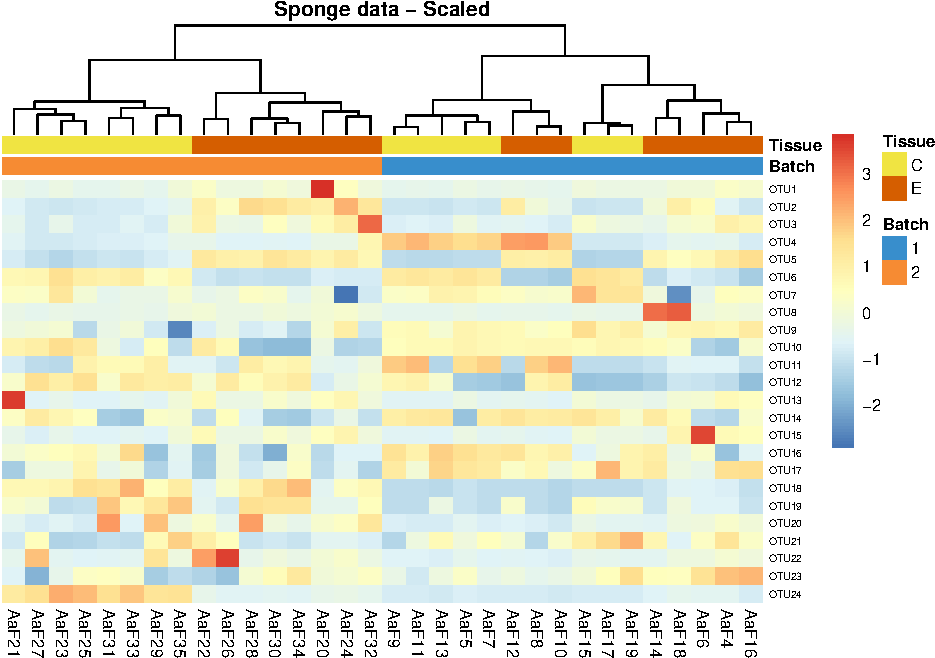
\includegraphics{Managing_batch_effects_files/figure-latex/unnamed-chunk-21-1.pdf}

In AD data, samples within batch 14/04/2016 are clustered and distinct
from other samples, also indicating a batch effect.

\begin{Shaded}
\begin{Highlighting}[]
\CommentTok{# HD data}
\NormalTok{hd.clr.scale <-}\StringTok{ }\KeywordTok{scale}\NormalTok{(hd.clr,}\DataTypeTok{center =}\NormalTok{ T, }\DataTypeTok{scale =}\NormalTok{ T)}
\NormalTok{hd.clr.scale <-}\StringTok{ }\KeywordTok{scale}\NormalTok{(}\KeywordTok{t}\NormalTok{(hd.clr.scale), }\DataTypeTok{center =}\NormalTok{ T, }\DataTypeTok{scale =}\NormalTok{ T)}

\NormalTok{hd.anno_col <-}\StringTok{ }\KeywordTok{data.frame}\NormalTok{(}\DataTypeTok{Batch =}\NormalTok{ hd.batch, }\DataTypeTok{Treatment =}\NormalTok{ hd.trt)}
\NormalTok{hd.anno_metabo_colors <-}\StringTok{ }\KeywordTok{list}\NormalTok{(}\DataTypeTok{Batch =} \KeywordTok{c}\NormalTok{(}\StringTok{'F'}\NormalTok{ =}\StringTok{ '#388ECC'}\NormalTok{, }\StringTok{'G'}\NormalTok{ =}\StringTok{ '#F68B33'}\NormalTok{,}
                                       \StringTok{'H'}\NormalTok{ =}\StringTok{ '#C2C2C2'}\NormalTok{, }\StringTok{'J'}\NormalTok{ =}\StringTok{ '#009E73'}\NormalTok{), }
                             \DataTypeTok{Treatment =} \KeywordTok{c}\NormalTok{(}\StringTok{'HD'}\NormalTok{ =}\StringTok{ '#0072B2'}\NormalTok{, }\StringTok{'WT'}\NormalTok{ =}\StringTok{ '#999999'}\NormalTok{))}


\KeywordTok{pheatmap}\NormalTok{(hd.clr.scale, }
         \DataTypeTok{scale =} \StringTok{'none'}\NormalTok{, }
         \DataTypeTok{cluster_rows =}\NormalTok{ F, }
         \DataTypeTok{cluster_cols =}\NormalTok{ T, }
         \DataTypeTok{fontsize_row =} \DecValTok{4}\NormalTok{, }\DataTypeTok{fontsize_col =} \DecValTok{6}\NormalTok{,}
         \DataTypeTok{fontsize =} \DecValTok{8}\NormalTok{,}
         \DataTypeTok{clustering_distance_rows =} \StringTok{'euclidean'}\NormalTok{,}
         \DataTypeTok{clustering_method =} \StringTok{'ward.D'}\NormalTok{,}
         \DataTypeTok{treeheight_row =} \DecValTok{30}\NormalTok{,}
         \DataTypeTok{annotation_col =}\NormalTok{ hd.anno_col,}
         \DataTypeTok{annotation_colors =}\NormalTok{ hd.anno_metabo_colors,}
         \DataTypeTok{border_color =} \StringTok{'NA'}\NormalTok{,}
         \DataTypeTok{main =} \StringTok{'HD data - Scaled'}\NormalTok{)}
\end{Highlighting}
\end{Shaded}

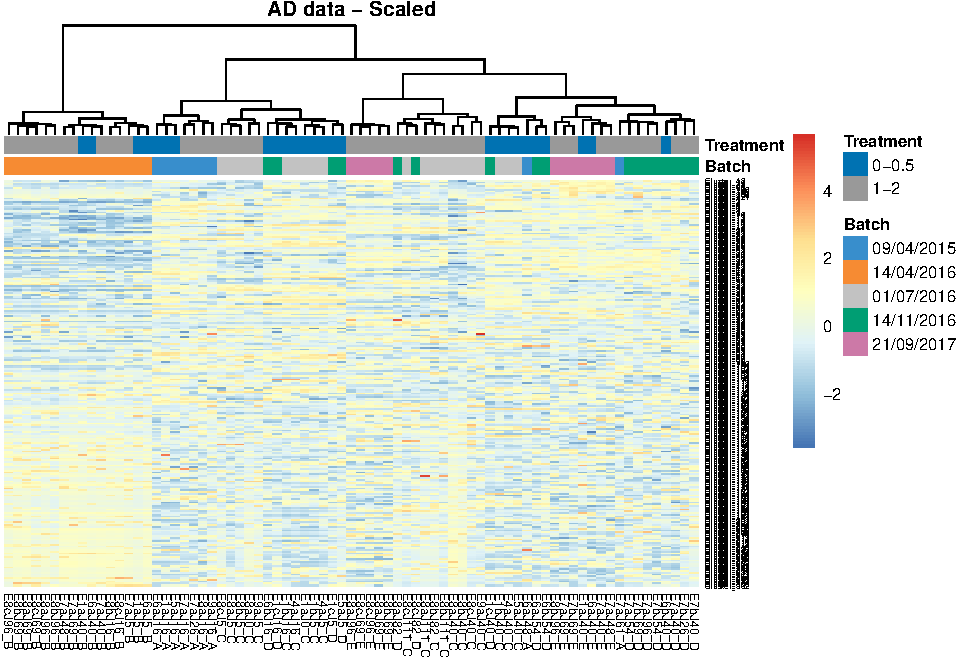
\includegraphics{Managing_batch_effects_files/figure-latex/unnamed-chunk-22-1.pdf}

The batch effect in HD data is not obvious in this heatmap, as we
observe not clustering according to batch.

\chapter{Batch effect adjustment}\label{adjust}

\section{Accounting for batch
effects}\label{accounting-for-batch-effects}

Methods that account for batch effects estimate unknown batch effects
through matrix decomposition and / or assign a known or estimated batch
as a covariate with linear models.

\subsection{Linear model and linear mixed
model}\label{linear-model-and-linear-mixed-model}

LM and LMM are suitable for known batch effects, and can consider batch
x treatment interaction and deal with unbalanced batch x treatment
design. But they are univariate and rely on a Gaussian likelihood
assumption, which may not apply to zero-inflated microbiome data despite
CLR transformation.

We fit a linear model with effect of interest and batch effect for each
OTU in both sponge and AD data. The P-value for the regression
coefficient associated with the \emph{effect of interest} in a linear
model is then extracted and multiple testing corrected with ``FDR''.

\begin{Shaded}
\begin{Highlighting}[]
\CommentTok{# Sponge data}
\NormalTok{sponge.trt_p <-}\StringTok{ }\KeywordTok{apply}\NormalTok{(sponge.tss.clr, }\DecValTok{2}\NormalTok{, }\DataTypeTok{FUN =} \ControlFlowTok{function}\NormalTok{(x)\{}
\NormalTok{  res.lm <-}\StringTok{ }\KeywordTok{lm}\NormalTok{(x }\OperatorTok{~}\StringTok{ }\NormalTok{sponge.trt }\OperatorTok{+}\StringTok{ }\NormalTok{sponge.batch)}
\NormalTok{  summary.res <-}\StringTok{ }\KeywordTok{summary}\NormalTok{(res.lm)}
\NormalTok{  p <-}\StringTok{ }\NormalTok{summary.res}\OperatorTok{$}\NormalTok{coefficients[}\DecValTok{2}\NormalTok{,}\DecValTok{4}\NormalTok{]}
\NormalTok{\})}

\NormalTok{sponge.trt_adjp <-}\StringTok{ }\KeywordTok{p.adjust}\NormalTok{(sponge.trt_p, }\DataTypeTok{method =} \StringTok{'fdr'}\NormalTok{)}

\CommentTok{# AD data}
\NormalTok{ad.trt_p <-}\StringTok{ }\KeywordTok{apply}\NormalTok{(ad.clr, }\DecValTok{2}\NormalTok{, }\DataTypeTok{FUN =} \ControlFlowTok{function}\NormalTok{(x)\{}
\NormalTok{  res.lm <-}\StringTok{ }\KeywordTok{lm}\NormalTok{(x }\OperatorTok{~}\StringTok{ }\NormalTok{ad.trt }\OperatorTok{+}\StringTok{ }\NormalTok{ad.batch)}
\NormalTok{  summary.res <-}\StringTok{ }\KeywordTok{summary}\NormalTok{(res.lm)}
\NormalTok{  p <-}\StringTok{ }\NormalTok{summary.res}\OperatorTok{$}\NormalTok{coefficients[}\DecValTok{2}\NormalTok{,}\DecValTok{4}\NormalTok{]}
\NormalTok{\})}

\NormalTok{ad.trt_adjp <-}\StringTok{ }\KeywordTok{p.adjust}\NormalTok{(ad.trt_p, }\DataTypeTok{method =} \StringTok{'fdr'}\NormalTok{)}
\end{Highlighting}
\end{Shaded}

As the batch x treatment design of HD data is unbalaced, we fit a linear
mixed model considering batch (cage) as random effects.

\begin{Shaded}
\begin{Highlighting}[]
\CommentTok{# HD data}
\NormalTok{hd.trt_p <-}\StringTok{ }\KeywordTok{apply}\NormalTok{(hd.clr, }\DecValTok{2}\NormalTok{, }\DataTypeTok{FUN =} \ControlFlowTok{function}\NormalTok{(x)\{}
\NormalTok{  res.lmm <-}\StringTok{ }\KeywordTok{lmer}\NormalTok{(x }\OperatorTok{~}\StringTok{ }\NormalTok{hd.trt }\OperatorTok{+}\StringTok{ }\NormalTok{(}\DecValTok{1}\OperatorTok{|}\NormalTok{hd.batch))}
\NormalTok{  summary.res <-}\StringTok{ }\KeywordTok{summary}\NormalTok{(res.lmm)}
\NormalTok{  p <-}\StringTok{ }\NormalTok{summary.res}\OperatorTok{$}\NormalTok{coefficients[}\DecValTok{2}\NormalTok{,}\DecValTok{5}\NormalTok{]}
\NormalTok{\})}

\NormalTok{hd.trt_adjp <-}\StringTok{ }\KeywordTok{p.adjust}\NormalTok{(hd.trt_p, }\DataTypeTok{method =} \StringTok{'fdr'}\NormalTok{)}
\end{Highlighting}
\end{Shaded}

\subsection{SVA}\label{sva}

SVA can account for unknown batch effects, but is a univariate approach
that relies on a Gaussian likelihood assumption and implicitly
introduces a correlation between treatment and batch.

The \emph{sva} function performs two different steps. First it
identifies the number of latent factors that need to be estimated. The
number of factors can be estimated using the function \emph{num.sv}.

We first fit a full model with effect of interest and a null model with
no effect, and use the full model in the function \emph{num.sv} to
estimate the number of latent factors.

\begin{Shaded}
\begin{Highlighting}[]
\CommentTok{# sponge data}
\NormalTok{sponge.mod <-}\StringTok{ }\KeywordTok{model.matrix}\NormalTok{( }\OperatorTok{~}\StringTok{ }\NormalTok{sponge.trt) }\CommentTok{# full model}
\NormalTok{sponge.mod0 <-}\StringTok{ }\KeywordTok{model.matrix}\NormalTok{( }\OperatorTok{~}\StringTok{ }\DecValTok{1}\NormalTok{,}\DataTypeTok{data =}\NormalTok{ sponge.trt) }\CommentTok{# null model}
\NormalTok{sponge.sva.n <-}\StringTok{ }\KeywordTok{num.sv}\NormalTok{(}\DataTypeTok{dat =} \KeywordTok{t}\NormalTok{(sponge.tss.clr), }\DataTypeTok{mod =}\NormalTok{ sponge.mod)}
\end{Highlighting}
\end{Shaded}

Next we apply the \emph{sva} function to estimate the surrogate
variables with both full and null models:

\begin{Shaded}
\begin{Highlighting}[]
\NormalTok{sponge.sva <-}\StringTok{ }\KeywordTok{sva}\NormalTok{(}\DataTypeTok{dat =} \KeywordTok{t}\NormalTok{(sponge.tss.clr), }\DataTypeTok{mod =}\NormalTok{ sponge.mod, }
                 \DataTypeTok{mod0 =}\NormalTok{ sponge.mod0, }\DataTypeTok{n.sv =}\NormalTok{ sponge.sva.n)}
\end{Highlighting}
\end{Shaded}

\begin{verbatim}
## Number of significant surrogate variables is:  3 
## Iteration (out of 5 ):1  2  3  4  5
\end{verbatim}

We then include the estimated surrogate variables in both the null and
full models. The reason is that we want to adjust for the surrogate
variables, so we treat them as adjustment variables that must be
included in both models. The \emph{f.pvalue} function is then used to
calculate parametric F-test P-values and Q-values (adjusted P-values)
for each OTU of sponge data.

\begin{Shaded}
\begin{Highlighting}[]
\NormalTok{sponge.mod.bat <-}\StringTok{ }\KeywordTok{cbind}\NormalTok{(sponge.mod, sponge.sva}\OperatorTok{$}\NormalTok{sv)}
\NormalTok{sponge.mod0.bat <-}\StringTok{ }\KeywordTok{cbind}\NormalTok{(sponge.mod0, sponge.sva}\OperatorTok{$}\NormalTok{sv)}

\NormalTok{sponge.sva.trt_p <-}\StringTok{ }\KeywordTok{f.pvalue}\NormalTok{(}\KeywordTok{t}\NormalTok{(sponge.tss.clr), sponge.mod.bat, sponge.mod0.bat)}
\NormalTok{sponge.sva.trt_adjp <-}\StringTok{ }\KeywordTok{p.adjust}\NormalTok{(sponge.sva.trt_p, }\DataTypeTok{method=}\StringTok{'fdr'}\NormalTok{)}
\end{Highlighting}
\end{Shaded}

Now these P-values and Q-values are accounting for surrogate variables
(estimated batch effects).

We also apply SVA on both AD and HD data.

\begin{Shaded}
\begin{Highlighting}[]
\CommentTok{# ad data}
\NormalTok{ad.mod <-}\StringTok{ }\KeywordTok{model.matrix}\NormalTok{( }\OperatorTok{~}\StringTok{ }\NormalTok{ad.trt)}
\NormalTok{ad.mod0 <-}\StringTok{ }\KeywordTok{model.matrix}\NormalTok{( }\OperatorTok{~}\StringTok{ }\DecValTok{1}\NormalTok{, }\DataTypeTok{data =}\NormalTok{ ad.trt)}
\NormalTok{ad.sva.n <-}\StringTok{ }\KeywordTok{num.sv}\NormalTok{(}\DataTypeTok{dat =} \KeywordTok{t}\NormalTok{(ad.clr), }\DataTypeTok{mod =}\NormalTok{ ad.mod)}
\NormalTok{ad.sva <-}\StringTok{ }\KeywordTok{sva}\NormalTok{(}\KeywordTok{t}\NormalTok{(ad.clr), ad.mod, ad.mod0, }\DataTypeTok{n.sv =}\NormalTok{ ad.sva.n)}
\end{Highlighting}
\end{Shaded}

\begin{verbatim}
## Number of significant surrogate variables is:  6 
## Iteration (out of 5 ):1  2  3  4  5
\end{verbatim}

\begin{Shaded}
\begin{Highlighting}[]
\NormalTok{ad.mod.bat <-}\StringTok{ }\KeywordTok{cbind}\NormalTok{(ad.mod, ad.sva}\OperatorTok{$}\NormalTok{sv)}
\NormalTok{ad.mod0.bat <-}\StringTok{ }\KeywordTok{cbind}\NormalTok{(ad.mod0, ad.sva}\OperatorTok{$}\NormalTok{sv)}
\NormalTok{ad.sva.trt_p <-}\StringTok{ }\KeywordTok{f.pvalue}\NormalTok{(}\KeywordTok{t}\NormalTok{(ad.clr), ad.mod.bat, ad.mod0.bat)}
\NormalTok{ad.sva.trt_adjp <-}\StringTok{ }\KeywordTok{p.adjust}\NormalTok{(ad.sva.trt_p, }\DataTypeTok{method =} \StringTok{'fdr'}\NormalTok{)}

\CommentTok{# hd data}
\NormalTok{hd.mod <-}\StringTok{ }\KeywordTok{model.matrix}\NormalTok{( }\OperatorTok{~}\StringTok{ }\NormalTok{hd.trt)}
\NormalTok{hd.mod0 <-}\StringTok{ }\KeywordTok{model.matrix}\NormalTok{( }\OperatorTok{~}\StringTok{ }\DecValTok{1}\NormalTok{,}\DataTypeTok{data =}\NormalTok{ hd.trt)}
\NormalTok{hd.sva.n <-}\StringTok{ }\KeywordTok{num.sv}\NormalTok{(}\DataTypeTok{dat =} \KeywordTok{t}\NormalTok{(hd.clr), }\DataTypeTok{mod =}\NormalTok{ hd.mod)}
\NormalTok{hd.sva <-}\StringTok{ }\KeywordTok{sva}\NormalTok{(}\KeywordTok{t}\NormalTok{(hd.clr), hd.mod, hd.mod0, }\DataTypeTok{n.sv =}\NormalTok{ hd.sva.n)}
\end{Highlighting}
\end{Shaded}

\begin{verbatim}
## Number of significant surrogate variables is:  3 
## Iteration (out of 5 ):1  2  3  4  5
\end{verbatim}

\begin{Shaded}
\begin{Highlighting}[]
\NormalTok{hd.mod.bat <-}\StringTok{ }\KeywordTok{cbind}\NormalTok{(hd.mod, hd.sva}\OperatorTok{$}\NormalTok{sv)}
\NormalTok{hd.mod0.bat <-}\StringTok{ }\KeywordTok{cbind}\NormalTok{(hd.mod0, hd.sva}\OperatorTok{$}\NormalTok{sv)}
\NormalTok{hd.sva.trt_p <-}\StringTok{ }\KeywordTok{f.pvalue}\NormalTok{(}\KeywordTok{t}\NormalTok{(hd.clr), hd.mod.bat, hd.mod0.bat)}
\NormalTok{hd.sva.trt_adjp <-}\StringTok{ }\KeywordTok{p.adjust}\NormalTok{(hd.sva.trt_p, }\DataTypeTok{method =} \StringTok{'fdr'}\NormalTok{)}
\end{Highlighting}
\end{Shaded}

\subsection{RUV2}\label{ruv2}

RUV2 estimates and accounts for unknown batch effects, but the method
requires negative control variables that are affected by batch effects
but not treatment effects.

Practically, negative control variables are chosen prior during the
experimental design so that they are not affected by treatments (and
assume they are affected by batch effects). RUV2 can only account for
the difference captured by these controls.

Since our three datasets do not have negative control variables, we use
a linear model (or linear mixed model) to identify OTUs that are not
affected by treatment, those will be considered as \emph{pseudo negative
control variables} to fit the assumptions of RUV2. The P-values of
treatment effects calculated in section `linear model and linear mixed
model' are therefore used here.

\textbf{Note:} This analysis is not optimal as we use \emph{pseudo
negative control variables}, but we wish to provide this as a practical
example.

\begin{Shaded}
\begin{Highlighting}[]
\CommentTok{# sponge data}
\NormalTok{sponge.nc <-}\StringTok{ }\NormalTok{sponge.trt_adjp }\OperatorTok{>}\StringTok{ }\FloatTok{0.05}

\CommentTok{# AD data}
\NormalTok{ad.nc <-}\StringTok{ }\NormalTok{ad.trt_adjp }\OperatorTok{>}\StringTok{ }\FloatTok{0.05}

\CommentTok{# HD data}
\NormalTok{hd.nc <-}\StringTok{ }\NormalTok{hd.trt_p }\OperatorTok{>}\StringTok{ }\FloatTok{0.05}
\end{Highlighting}
\end{Shaded}

\textbf{Note:} In HD data, there is no OTU having statistically
siginificant difference between genotypes. We use P-values instead of
adjusted P-values to set the negative controls.

We then apply the \emph{RUV2} function. This function needs to specify
the number of unwanted factors (components of negative controls), which
we arbitrarily set to k = 3. We then extract the P-values of treatment
effects considering unwanted batch effects after FDR adjustment.

\begin{Shaded}
\begin{Highlighting}[]
\CommentTok{# sponge data}
\NormalTok{sponge.ruv2 <-}\StringTok{ }\KeywordTok{RUV2}\NormalTok{(}\DataTypeTok{Y =}\NormalTok{ sponge.tss.clr, }\DataTypeTok{X =}\NormalTok{ sponge.trt, }
                    \DataTypeTok{ctl =}\NormalTok{ sponge.nc, }\DataTypeTok{k =} \DecValTok{3}\NormalTok{) }\CommentTok{# k is subjective}
\NormalTok{sponge.ruv2.trt_p <-}\StringTok{ }\NormalTok{sponge.ruv2}\OperatorTok{$}\NormalTok{p}
\NormalTok{sponge.ruv2.trt_adjp <-}\StringTok{ }\KeywordTok{p.adjust}\NormalTok{(sponge.ruv2.trt_p, }\DataTypeTok{method=}\StringTok{"fdr"}\NormalTok{)}

\CommentTok{# AD data}
\NormalTok{ad.ruv2 <-}\StringTok{ }\KeywordTok{RUV2}\NormalTok{(}\DataTypeTok{Y =}\NormalTok{ ad.clr, }\DataTypeTok{X =}\NormalTok{ ad.trt, }
                \DataTypeTok{ctl =}\NormalTok{ ad.nc, }\DataTypeTok{k =} \DecValTok{3}\NormalTok{) }\CommentTok{# k is subjective}
\NormalTok{ad.ruv2.trt_p <-}\StringTok{ }\NormalTok{ad.ruv2}\OperatorTok{$}\NormalTok{p}
\NormalTok{ad.ruv2.trt_adjp <-}\StringTok{ }\KeywordTok{p.adjust}\NormalTok{(ad.ruv2.trt_p, }\DataTypeTok{method=}\StringTok{"fdr"}\NormalTok{)}

\CommentTok{# HD data}
\NormalTok{hd.ruv2 <-}\StringTok{ }\KeywordTok{RUV2}\NormalTok{(}\DataTypeTok{Y =}\NormalTok{ hd.clr, }\DataTypeTok{X =}\NormalTok{ hd.trt, }
                \DataTypeTok{ctl =}\NormalTok{ hd.nc, }\DataTypeTok{k =} \DecValTok{3}\NormalTok{) }\CommentTok{# k is subjective}
\NormalTok{hd.ruv2.trt_p <-}\StringTok{ }\NormalTok{hd.ruv2}\OperatorTok{$}\NormalTok{p}
\NormalTok{hd.ruv2.trt_adjp <-}\StringTok{ }\KeywordTok{p.adjust}\NormalTok{(hd.ruv2.trt_p, }\DataTypeTok{method=}\StringTok{"fdr"}\NormalTok{)}
\end{Highlighting}
\end{Shaded}

\subsection{RUV4}\label{ruv4}

RUV4 is an updated version of RUV2 that uses negative control variables
and the residual matrix that has no treatment effect to estimate
unwanted batch effects.

\emph{RUV4} also requires to specify the number of unwanted factors as
\emph{RUV2}, which we estimate with the function \emph{`getK'} (from the
\emph{ruv} package). This function is only for \emph{RUV4} and the
estimated k is not always suitable. If the estimated k is 0, k can be
set to 1 instead to account for unwanted variation captured from
negative controls.

\begin{Shaded}
\begin{Highlighting}[]
\CommentTok{# sponge data}
\NormalTok{sponge.k.obj <-}\StringTok{ }\KeywordTok{getK}\NormalTok{(}\DataTypeTok{Y =}\NormalTok{ sponge.tss.clr, }\DataTypeTok{X =}\NormalTok{ sponge.trt, }\DataTypeTok{ctl =}\NormalTok{ sponge.nc)}
\NormalTok{sponge.k <-}\StringTok{ }\NormalTok{sponge.k.obj}\OperatorTok{$}\NormalTok{k}
\NormalTok{sponge.k <-}\StringTok{ }\KeywordTok{ifelse}\NormalTok{(sponge.k }\OperatorTok{!=}\DecValTok{0}\NormalTok{, sponge.k, }\DecValTok{1}\NormalTok{)}
\NormalTok{sponge.ruv4 <-}\StringTok{ }\KeywordTok{RUV4}\NormalTok{(}\DataTypeTok{Y =}\NormalTok{ sponge.tss.clr, }\DataTypeTok{X =}\NormalTok{ sponge.trt, }\DataTypeTok{ctl =}\NormalTok{ sponge.nc, }\DataTypeTok{k =}\NormalTok{ sponge.k) }
\NormalTok{sponge.ruv4.trt_p <-}\StringTok{ }\NormalTok{sponge.ruv4}\OperatorTok{$}\NormalTok{p}
\NormalTok{sponge.ruv4.trt_adjp <-}\StringTok{ }\KeywordTok{p.adjust}\NormalTok{(sponge.ruv4.trt_p, }\DataTypeTok{method=}\StringTok{"fdr"}\NormalTok{)}

\CommentTok{# AD data}
\NormalTok{ad.k.obj <-}\StringTok{ }\KeywordTok{getK}\NormalTok{(}\DataTypeTok{Y =}\NormalTok{ ad.clr, }\DataTypeTok{X =}\NormalTok{ ad.trt, }\DataTypeTok{ctl =}\NormalTok{ ad.nc)}
\NormalTok{ad.k <-}\StringTok{ }\NormalTok{ad.k.obj}\OperatorTok{$}\NormalTok{k}
\NormalTok{ad.k <-}\StringTok{ }\KeywordTok{ifelse}\NormalTok{(ad.k }\OperatorTok{!=}\DecValTok{0}\NormalTok{, ad.k, }\DecValTok{1}\NormalTok{)}
\NormalTok{ad.ruv4 <-}\StringTok{ }\KeywordTok{RUV4}\NormalTok{(}\DataTypeTok{Y =}\NormalTok{ ad.clr, }\DataTypeTok{X =}\NormalTok{ ad.trt, }\DataTypeTok{ctl =}\NormalTok{ ad.nc, }\DataTypeTok{k =}\NormalTok{ ad.k) }
\NormalTok{ad.ruv4.trt_p <-}\StringTok{ }\NormalTok{ad.ruv4}\OperatorTok{$}\NormalTok{p}
\NormalTok{ad.ruv4.trt_adjp <-}\StringTok{ }\KeywordTok{p.adjust}\NormalTok{(ad.ruv4.trt_p, }\DataTypeTok{method=}\StringTok{"fdr"}\NormalTok{)}

\CommentTok{# HD data}
\NormalTok{hd.k.obj <-}\StringTok{ }\KeywordTok{getK}\NormalTok{(}\DataTypeTok{Y =}\NormalTok{ hd.clr, }\DataTypeTok{X =}\NormalTok{ hd.trt, }\DataTypeTok{ctl =}\NormalTok{ hd.nc)}
\NormalTok{hd.k <-}\StringTok{ }\NormalTok{hd.k.obj}\OperatorTok{$}\NormalTok{k}
\NormalTok{hd.k <-}\StringTok{ }\KeywordTok{ifelse}\NormalTok{(hd.k }\OperatorTok{!=}\DecValTok{0}\NormalTok{, hd.k, }\DecValTok{1}\NormalTok{)}
\NormalTok{hd.ruv4 <-}\StringTok{ }\KeywordTok{RUV4}\NormalTok{(}\DataTypeTok{Y =}\NormalTok{ hd.clr, }\DataTypeTok{X =}\NormalTok{ hd.trt, }\DataTypeTok{ctl =}\NormalTok{ hd.nc, }\DataTypeTok{k =}\NormalTok{ hd.k) }
\NormalTok{hd.ruv4.trt_p <-}\StringTok{ }\NormalTok{hd.ruv4}\OperatorTok{$}\NormalTok{p}
\NormalTok{hd.ruv4.trt_adjp <-}\StringTok{ }\KeywordTok{p.adjust}\NormalTok{(hd.ruv4.trt_p, }\DataTypeTok{method=}\StringTok{"fdr"}\NormalTok{)}
\end{Highlighting}
\end{Shaded}

\section{Correcting for batch
effects}\label{correcting-for-batch-effects}

An alternative approach to manage batch effects is to remove batch
effects from the original microbiome data, then use the corrected data
in any subsequent data analysis. Compared with methods accounting for
batch effects, batch effect correction methods are practical and enable
broader application in a variety of analyses. However, the methods do
not consider the correlation (linear) and interaction (non-linear)
between batch and treatment effects and may result in over-adjusted
batch effects, statistical power loss, and an inability to detect
variables associated with the treatment effect.

\subsection{BMC (batch mean centering)}\label{bmc-batch-mean-centering}

We center data within a batch across all variables. As a result, each
batch mean is standardised to zero. BMC has several disadvantages: it is
a univariate method and it is not optimal for non-Gaussian distributed
microbiome data.

\begin{Shaded}
\begin{Highlighting}[]
\CommentTok{# Sponge data}
\NormalTok{sponge.b1 <-}\StringTok{ }\KeywordTok{scale}\NormalTok{(sponge.tss.clr[sponge.batch }\OperatorTok{==}\StringTok{ }\DecValTok{1}\NormalTok{, ], }\DataTypeTok{center =} \OtherTok{TRUE}\NormalTok{, }\DataTypeTok{scale =} \OtherTok{FALSE}\NormalTok{)}
\NormalTok{sponge.b2 <-}\StringTok{ }\KeywordTok{scale}\NormalTok{(sponge.tss.clr[sponge.batch }\OperatorTok{==}\StringTok{ }\DecValTok{2}\NormalTok{, ], }\DataTypeTok{center =} \OtherTok{TRUE}\NormalTok{, }\DataTypeTok{scale =} \OtherTok{FALSE}\NormalTok{)}
\NormalTok{sponge.bmc <-}\StringTok{ }\KeywordTok{rbind}\NormalTok{(sponge.b1, sponge.b2)}
\NormalTok{sponge.bmc <-}\StringTok{ }\NormalTok{sponge.bmc[}\KeywordTok{rownames}\NormalTok{(sponge.tss.clr), ]}
\end{Highlighting}
\end{Shaded}

\begin{Shaded}
\begin{Highlighting}[]
\CommentTok{# AD data}
\NormalTok{ad.b1 <-}\StringTok{ }\KeywordTok{scale}\NormalTok{(ad.clr[ad.batch }\OperatorTok{==}\StringTok{ '09/04/2015'}\NormalTok{, ], }\DataTypeTok{center =} \OtherTok{TRUE}\NormalTok{, }\DataTypeTok{scale =} \OtherTok{FALSE}\NormalTok{)}
\NormalTok{ad.b2 <-}\StringTok{ }\KeywordTok{scale}\NormalTok{(ad.clr[ad.batch }\OperatorTok{==}\StringTok{ '14/04/2016'}\NormalTok{, ], }\DataTypeTok{center =} \OtherTok{TRUE}\NormalTok{, }\DataTypeTok{scale =} \OtherTok{FALSE}\NormalTok{)}
\NormalTok{ad.b3 <-}\StringTok{ }\KeywordTok{scale}\NormalTok{(ad.clr[ad.batch }\OperatorTok{==}\StringTok{ '14/11/2016'}\NormalTok{, ], }\DataTypeTok{center =} \OtherTok{TRUE}\NormalTok{, }\DataTypeTok{scale =} \OtherTok{FALSE}\NormalTok{)}
\NormalTok{ad.b4 <-}\StringTok{ }\KeywordTok{scale}\NormalTok{(ad.clr[ad.batch }\OperatorTok{==}\StringTok{ '01/07/2016'}\NormalTok{, ], }\DataTypeTok{center =} \OtherTok{TRUE}\NormalTok{, }\DataTypeTok{scale =} \OtherTok{FALSE}\NormalTok{)}
\NormalTok{ad.b5 <-}\StringTok{ }\KeywordTok{scale}\NormalTok{(ad.clr[ad.batch }\OperatorTok{==}\StringTok{ '21/09/2017'}\NormalTok{, ], }\DataTypeTok{center =} \OtherTok{TRUE}\NormalTok{, }\DataTypeTok{scale =} \OtherTok{FALSE}\NormalTok{)}
\NormalTok{ad.bmc <-}\StringTok{ }\KeywordTok{rbind}\NormalTok{(ad.b1, ad.b2, ad.b3, ad.b4, ad.b5)}
\NormalTok{ad.bmc <-}\StringTok{ }\NormalTok{ad.bmc[}\KeywordTok{rownames}\NormalTok{(ad.clr), ]}
\end{Highlighting}
\end{Shaded}

\subsection{ComBat}\label{combat}

ComBat requires known and systematic batch effects. If the treatment
information is known, the option \emph{mod} can be fitted with a full
model having treatment informationn to efficiently maintain enough
treatment variation (see examples below for sponge and AD data). The
\emph{mod} can also be NULL if the treatment information is unknown.

\begin{Shaded}
\begin{Highlighting}[]
\CommentTok{# Sponge data}
\NormalTok{sponge.combat <-}\StringTok{ }\KeywordTok{t}\NormalTok{(}\KeywordTok{ComBat}\NormalTok{(}\KeywordTok{t}\NormalTok{(sponge.tss.clr), }\DataTypeTok{batch =}\NormalTok{ sponge.batch, }
                          \DataTypeTok{mod =}\NormalTok{ sponge.mod, }\DataTypeTok{par.prior =}\NormalTok{ F, }\DataTypeTok{prior.plots =}\NormalTok{ F))}
\end{Highlighting}
\end{Shaded}

\begin{verbatim}
## Found2batches
\end{verbatim}

\begin{verbatim}
## Adjusting for1covariate(s) or covariate level(s)
\end{verbatim}

\begin{verbatim}
## Standardizing Data across genes
\end{verbatim}

\begin{verbatim}
## Fitting L/S model and finding priors
\end{verbatim}

\begin{verbatim}
## Finding nonparametric adjustments
\end{verbatim}

\begin{verbatim}
## Adjusting the Data
\end{verbatim}

\begin{Shaded}
\begin{Highlighting}[]
\CommentTok{# AD data}
\NormalTok{ad.combat <-}\StringTok{ }\KeywordTok{t}\NormalTok{(}\KeywordTok{ComBat}\NormalTok{(}\KeywordTok{t}\NormalTok{(ad.clr), }\DataTypeTok{batch =}\NormalTok{ ad.batch, }
                      \DataTypeTok{mod =}\NormalTok{ ad.mod, }\DataTypeTok{par.prior =}\NormalTok{ F, }\DataTypeTok{prior.plots =}\NormalTok{ F))}
\end{Highlighting}
\end{Shaded}

\begin{verbatim}
## Found5batches
\end{verbatim}

\begin{verbatim}
## Adjusting for1covariate(s) or covariate level(s)
\end{verbatim}

\begin{verbatim}
## Standardizing Data across genes
\end{verbatim}

\begin{verbatim}
## Fitting L/S model and finding priors
\end{verbatim}

\begin{verbatim}
## Finding nonparametric adjustments
\end{verbatim}

\begin{verbatim}
## Adjusting the Data
\end{verbatim}

\subsection{removeBatchEffect}\label{removebatcheffect}

\emph{removeBatchEffect} is a function implemented in the LIMMA package
that fits a linear model for each variable given a series of conditions
as explanatory variables, including the batch effect and treatment
effect. Contrary to a standard linear or linear mixed models (see
section `linear model and linear mixed model') that simultaneously
estimate treatment and batch effects, \emph{removeBatchEffect} subtracts
the batch effect from the original data, resulting in a residual matrix
that contains any and only treatment effect. The option \emph{design} is
the same as option \emph{mod} in ComBat.

\begin{Shaded}
\begin{Highlighting}[]
\CommentTok{# Sponge data}
\NormalTok{sponge.limma <-}\StringTok{ }\KeywordTok{t}\NormalTok{(}\KeywordTok{removeBatchEffect}\NormalTok{(}\KeywordTok{t}\NormalTok{(sponge.tss.clr), }\DataTypeTok{batch =}\NormalTok{ sponge.batch, }
                                    \DataTypeTok{design =}\NormalTok{ sponge.mod))}
\end{Highlighting}
\end{Shaded}

\begin{Shaded}
\begin{Highlighting}[]
\NormalTok{ad.limma <-}\StringTok{ }\KeywordTok{t}\NormalTok{(}\KeywordTok{removeBatchEffect}\NormalTok{(}\KeywordTok{t}\NormalTok{(ad.clr), }\DataTypeTok{batch =}\NormalTok{ ad.batch, }
                                \DataTypeTok{design =}\NormalTok{ ad.mod))}
\end{Highlighting}
\end{Shaded}

\subsection{FAbatch}\label{fabatch}

FAbatch is a combination of location-scale adjustment and factor
analysis. We fit \emph{y} with the treatment information and
\emph{batch} with batch information. Since this method only accepts
numeric variables, the levels of variables are changed to be numeric
(e.g. `1', `2' and so on). However, on our example, FAbatch did not
converge, potentially leading to suboptimal results. We therefore did
not compare the results from FAbatch with those from other methods.

\begin{Shaded}
\begin{Highlighting}[]
\CommentTok{# sponge data}
\NormalTok{sponge.fabatch.obj <-}\StringTok{ }\KeywordTok{fabatch}\NormalTok{(}\DataTypeTok{x =}\NormalTok{ sponge.tss.clr, }
                             \DataTypeTok{y =} \KeywordTok{as.factor}\NormalTok{(}\KeywordTok{as.numeric}\NormalTok{(sponge.trt)), }
                             \DataTypeTok{batch =}\NormalTok{ sponge.batch)}
\NormalTok{sponge.fabatch <-}\StringTok{ }\NormalTok{sponge.fabatch.obj}\OperatorTok{$}\NormalTok{xadj}

\CommentTok{# ad data}
\NormalTok{ad.fabatch.obj <-}\StringTok{ }\KeywordTok{fabatch}\NormalTok{(}\DataTypeTok{x =}\NormalTok{ ad.clr, }
                         \DataTypeTok{y =} \KeywordTok{as.factor}\NormalTok{(}\KeywordTok{as.numeric}\NormalTok{(ad.trt)), }
                         \DataTypeTok{batch =} \KeywordTok{as.factor}\NormalTok{(}\KeywordTok{as.numeric}\NormalTok{(ad.batch)))}
\NormalTok{ad.fabatch <-}\StringTok{ }\NormalTok{ad.fabatch.obj}\OperatorTok{$}\NormalTok{xadj}
\end{Highlighting}
\end{Shaded}

\subsection{Percentile normalisation}\label{percentile-normalisation}

Percentile normalisation (PN) was developed for microbiome data
integration. For each batch, it transforms the relative abundance of
control samples to their own percentiles while converting the relative
abundance of case samples into the percentiles of their corresponding
control distribution. The method thus only applies to case-control
studies, and may lose a large amount of information as it uses
percentiles rather than the original values.

\textbf{Note:} PN applies on TSS scaled data
\citep{gibbons2018correcting}. As we added an offset on sponge TSS
scaled data, we re-applied the TSS.

\begin{Shaded}
\begin{Highlighting}[]
\CommentTok{# sponge data}
\NormalTok{sponge.tss <-}\StringTok{ }\KeywordTok{t}\NormalTok{(}\KeywordTok{apply}\NormalTok{(sponge.tss, }\DecValTok{1}\NormalTok{, }\ControlFlowTok{function}\NormalTok{(x)\{x}\OperatorTok{/}\KeywordTok{sum}\NormalTok{(x)\}))}
\NormalTok{sponge.percentile <-}\StringTok{ }\KeywordTok{percentile_norm}\NormalTok{(}\DataTypeTok{data =}\NormalTok{ sponge.tss, }\DataTypeTok{batch =}\NormalTok{ sponge.batch, }
                                    \DataTypeTok{trt =}\NormalTok{ sponge.trt)}


\CommentTok{# ad data}
\CommentTok{# TSS}
\NormalTok{ad.tss <-}\StringTok{ }\KeywordTok{t}\NormalTok{(}\KeywordTok{apply}\NormalTok{(ad.count.keep, }\DecValTok{1}\NormalTok{, }\ControlFlowTok{function}\NormalTok{(x)\{x}\OperatorTok{/}\KeywordTok{sum}\NormalTok{(x)\}))}
\NormalTok{ad.percentile <-}\StringTok{ }\KeywordTok{percentile_norm}\NormalTok{(}\DataTypeTok{data =}\NormalTok{ ad.tss, }\DataTypeTok{batch =}\NormalTok{ ad.batch, }
                                \DataTypeTok{trt =}\NormalTok{ ad.trt)}
\end{Highlighting}
\end{Shaded}

\subsection{SVD-based method}\label{svd-based-method}

We center and scale the data before SVD. After SVD, we deflate the first
component, which has the highest variation and is assumed to be related
to batch effects.

\begin{Shaded}
\begin{Highlighting}[]
\CommentTok{# sponge data}
\NormalTok{sponge.sd <-}\StringTok{ }\KeywordTok{apply}\NormalTok{(sponge.tss.clr, }\DecValTok{2}\NormalTok{, sd) }\CommentTok{# calculate standard deviation}
\NormalTok{sponge.mean <-}\StringTok{ }\KeywordTok{apply}\NormalTok{(sponge.tss.clr, }\DecValTok{2}\NormalTok{, mean) }\CommentTok{# calculate mean}
\NormalTok{sponge.X <-}\StringTok{ }\KeywordTok{scale}\NormalTok{(sponge.tss.clr, }\DataTypeTok{center =}\NormalTok{ T, }\DataTypeTok{scale =}\NormalTok{ T) }\CommentTok{# center and scale}

\NormalTok{sponge.m <-}\StringTok{ }\KeywordTok{crossprod}\NormalTok{(sponge.X) }\CommentTok{# generate a square matrix}
\NormalTok{sponge.m.svd <-}\StringTok{ }\KeywordTok{svd}\NormalTok{(sponge.m) }\CommentTok{# SVD }
\CommentTok{# barplot(sponge.m.svd$d)}

\CommentTok{# extract 1st singular vectors}
\NormalTok{sponge.a1 <-}\StringTok{ }\NormalTok{sponge.m.svd}\OperatorTok{$}\NormalTok{u[ ,}\DecValTok{1}\NormalTok{] }
\NormalTok{sponge.b1 <-}\StringTok{ }\NormalTok{sponge.m.svd}\OperatorTok{$}\NormalTok{v[ ,}\DecValTok{1}\NormalTok{]}

\CommentTok{# deflate component 1 from the data}
\NormalTok{sponge.t1 <-}\StringTok{ }\NormalTok{sponge.X }\OperatorTok\StringTok{ }\NormalTok{sponge.a1 }\OperatorTok{/}\StringTok{ }\KeywordTok{drop}\NormalTok{(}\KeywordTok{sqrt}\NormalTok{(}\KeywordTok{crossprod}\NormalTok{(sponge.a1)))}
\NormalTok{sponge.c1 <-}\StringTok{ }\KeywordTok{crossprod}\NormalTok{(sponge.X, sponge.t1) }\OperatorTok{/}\StringTok{ }\KeywordTok{drop}\NormalTok{(}\KeywordTok{crossprod}\NormalTok{(sponge.t1))}
\NormalTok{sponge.svd.defl.matrix1  <-}\StringTok{ }\NormalTok{sponge.X }\OperatorTok{-}\StringTok{ }\NormalTok{sponge.t1 }\OperatorTok\StringTok{ }\KeywordTok{t}\NormalTok{(sponge.c1)}

\CommentTok{# add back mean and standard deviation}
\NormalTok{sponge.svd <-}\StringTok{ }\NormalTok{sponge.svd.defl.matrix1}
\NormalTok{sponge.svd[}\DecValTok{1}\OperatorTok{:}\KeywordTok{nrow}\NormalTok{(sponge.svd), }\DecValTok{1}\OperatorTok{:}\KeywordTok{ncol}\NormalTok{(sponge.svd)] =}\StringTok{ }\OtherTok{NA}
\ControlFlowTok{for}\NormalTok{(i }\ControlFlowTok{in} \DecValTok{1}\OperatorTok{:}\KeywordTok{ncol}\NormalTok{(sponge.svd.defl.matrix1))\{}
  \ControlFlowTok{for}\NormalTok{(j }\ControlFlowTok{in} \DecValTok{1}\OperatorTok{:}\KeywordTok{nrow}\NormalTok{(sponge.svd.defl.matrix1))\{}
\NormalTok{    sponge.svd[j,i] =}\StringTok{ }\NormalTok{sponge.svd.defl.matrix1[j,i]}\OperatorTok{*}\NormalTok{sponge.sd[i] }\OperatorTok{+}\StringTok{ }\NormalTok{sponge.mean[i]}
\NormalTok{  \}}
\NormalTok{\}}
\end{Highlighting}
\end{Shaded}

\begin{Shaded}
\begin{Highlighting}[]
\CommentTok{# ad data}
\NormalTok{ad.sd <-}\StringTok{ }\KeywordTok{apply}\NormalTok{(ad.clr, }\DecValTok{2}\NormalTok{, sd) }\CommentTok{# calculate standard deviation}
\NormalTok{ad.mean <-}\StringTok{ }\KeywordTok{apply}\NormalTok{(ad.clr, }\DecValTok{2}\NormalTok{, mean) }\CommentTok{# calculate mean}
\NormalTok{ad.X <-}\StringTok{ }\KeywordTok{scale}\NormalTok{(ad.clr,}\DataTypeTok{center =}\NormalTok{ T, }\DataTypeTok{scale =}\NormalTok{ T) }\CommentTok{# center and scale}

\NormalTok{ad.m <-}\StringTok{ }\KeywordTok{crossprod}\NormalTok{(ad.X) }\CommentTok{# generate a square matrix}
\NormalTok{ad.m.svd <-}\StringTok{ }\KeywordTok{svd}\NormalTok{(ad.m) }\CommentTok{# SVD }
\CommentTok{# barplot(ad.m.svd$d)}

\CommentTok{# extract 1st singular vectors}
\NormalTok{ad.a1 <-}\StringTok{ }\NormalTok{ad.m.svd}\OperatorTok{$}\NormalTok{u[ ,}\DecValTok{1}\NormalTok{]}
\NormalTok{ad.b1 <-}\StringTok{ }\NormalTok{ad.m.svd}\OperatorTok{$}\NormalTok{v[ ,}\DecValTok{1}\NormalTok{]}

\CommentTok{# deflate component 1 from the data}
\NormalTok{ad.t1 <-}\StringTok{ }\NormalTok{ad.X }\OperatorTok\StringTok{ }\NormalTok{ad.a1 }\OperatorTok{/}\StringTok{ }\KeywordTok{drop}\NormalTok{(}\KeywordTok{sqrt}\NormalTok{(}\KeywordTok{crossprod}\NormalTok{(ad.a1)))}
\NormalTok{ad.c1 <-}\StringTok{ }\KeywordTok{crossprod}\NormalTok{(ad.X, ad.t1) }\OperatorTok{/}\StringTok{ }\KeywordTok{drop}\NormalTok{(}\KeywordTok{crossprod}\NormalTok{(ad.t1))}
\NormalTok{ad.svd.defl.matrix1  <-}\StringTok{ }\NormalTok{ad.X }\OperatorTok{-}\StringTok{ }\NormalTok{ad.t1 }\OperatorTok\StringTok{ }\KeywordTok{t}\NormalTok{(ad.c1)}

\CommentTok{# add back mean and standard deviation}
\NormalTok{ad.svd <-}\StringTok{ }\NormalTok{ad.svd.defl.matrix1}
\NormalTok{ad.svd[}\DecValTok{1}\OperatorTok{:}\KeywordTok{nrow}\NormalTok{(ad.svd), }\DecValTok{1}\OperatorTok{:}\KeywordTok{ncol}\NormalTok{(ad.svd)] =}\StringTok{ }\OtherTok{NA}
\ControlFlowTok{for}\NormalTok{(i }\ControlFlowTok{in} \DecValTok{1}\OperatorTok{:}\KeywordTok{ncol}\NormalTok{(ad.svd.defl.matrix1))\{}
  \ControlFlowTok{for}\NormalTok{(j }\ControlFlowTok{in} \DecValTok{1}\OperatorTok{:}\KeywordTok{nrow}\NormalTok{(ad.svd.defl.matrix1))\{}
\NormalTok{    ad.svd[j,i] =}\StringTok{ }\NormalTok{ad.svd.defl.matrix1[j,i]}\OperatorTok{*}\NormalTok{ad.sd[i] }\OperatorTok{+}\StringTok{ }\NormalTok{ad.mean[i]}
\NormalTok{  \}}
\NormalTok{\}}
\end{Highlighting}
\end{Shaded}

\subsection{RUVIII}\label{ruviii}

RUVIII needs not only negative control variables as RUV2 and RUV4, but
also technical sample replicates. As only AD data include sample
replicates, we illustrate RUVIII on these data only.

In contrast to RUV2 and RUV4, RUVIII is a multivariate method that
accounts for the dependency between microbial variables, but it is
currently limited to the correction of technical and computational
sources of batch effects.

\textbf{Note:} RUVIII requires the number of negative control variables
to be larger than the sample size in order to fully use the sample
information.

\begin{Shaded}
\begin{Highlighting}[]
\CommentTok{# ad data only}
\NormalTok{ad.replicates <-}\StringTok{ }\NormalTok{ad.metadata}\OperatorTok{$}\NormalTok{sample_name.data.extraction}
\NormalTok{ad.replicates.matrix <-}\StringTok{ }\KeywordTok{replicate.matrix}\NormalTok{(ad.replicates)}

\NormalTok{ad.ruvIII <-}\StringTok{ }\KeywordTok{RUVIII}\NormalTok{(}\DataTypeTok{Y =}\NormalTok{ ad.clr, }\DataTypeTok{M =}\NormalTok{ ad.replicates.matrix, }\DataTypeTok{ctl =}\NormalTok{ ad.nc)}
\KeywordTok{rownames}\NormalTok{(ad.ruvIII) <-}\StringTok{ }\KeywordTok{rownames}\NormalTok{(ad.clr)}
\end{Highlighting}
\end{Shaded}

\chapter{Methods evaluation}\label{eval}

After batch effect adjustment, it is essential to evaluate its
effectiveness. For simplicity, we focus only on strategies to assess
batch effect \emph{correction} methods, as methods that account for the
batch effect often imply it has been assessed internally in the
statistical model.

\section{Diagnostic plots}\label{diagnostic-plots}

Diagnostic plots are useful to visually evaluate for post-correction
batch effects, as presented earlier in section `batch effect detection'.

\subsection{Principal component analysis (PCA) with density plot per
component}\label{principal-component-analysis-pca-with-density-plot-per-component-1}

We apply PCA on both sponge and AD data before and after correction with
different methods.

\begin{Shaded}
\begin{Highlighting}[]
\CommentTok{# sponge data}
\NormalTok{sponge.pca.before <-}\StringTok{ }\KeywordTok{pca}\NormalTok{(sponge.tss.clr, }\DataTypeTok{ncomp =} \DecValTok{3}\NormalTok{)}
\NormalTok{sponge.pca.bmc <-}\StringTok{ }\KeywordTok{pca}\NormalTok{(sponge.bmc, }\DataTypeTok{ncomp =} \DecValTok{3}\NormalTok{)}
\NormalTok{sponge.pca.combat <-}\StringTok{ }\KeywordTok{pca}\NormalTok{(sponge.combat, }\DataTypeTok{ncomp =} \DecValTok{3}\NormalTok{)}
\NormalTok{sponge.pca.limma <-}\StringTok{ }\KeywordTok{pca}\NormalTok{(sponge.limma, }\DataTypeTok{ncomp =} \DecValTok{3}\NormalTok{)}
\NormalTok{sponge.pca.percentile <-}\StringTok{ }\KeywordTok{pca}\NormalTok{(sponge.percentile, }\DataTypeTok{ncomp =} \DecValTok{3}\NormalTok{)}
\NormalTok{sponge.pca.svd <-}\StringTok{ }\KeywordTok{pca}\NormalTok{(sponge.svd, }\DataTypeTok{ncomp =} \DecValTok{3}\NormalTok{)}

\CommentTok{# ad data}
\NormalTok{ad.pca.before <-}\StringTok{ }\KeywordTok{pca}\NormalTok{(ad.clr, }\DataTypeTok{ncomp =} \DecValTok{3}\NormalTok{)}
\NormalTok{ad.pca.bmc <-}\StringTok{ }\KeywordTok{pca}\NormalTok{(ad.bmc, }\DataTypeTok{ncomp =} \DecValTok{3}\NormalTok{)}
\NormalTok{ad.pca.combat <-}\StringTok{ }\KeywordTok{pca}\NormalTok{(ad.combat, }\DataTypeTok{ncomp =} \DecValTok{3}\NormalTok{)}
\NormalTok{ad.pca.limma <-}\StringTok{ }\KeywordTok{pca}\NormalTok{(ad.limma, }\DataTypeTok{ncomp =} \DecValTok{3}\NormalTok{)}
\NormalTok{ad.pca.percentile <-}\StringTok{ }\KeywordTok{pca}\NormalTok{(ad.percentile, }\DataTypeTok{ncomp =} \DecValTok{3}\NormalTok{)}
\NormalTok{ad.pca.svd <-}\StringTok{ }\KeywordTok{pca}\NormalTok{(ad.svd, }\DataTypeTok{ncomp =} \DecValTok{3}\NormalTok{)}
\NormalTok{ad.pca.ruv <-}\StringTok{ }\KeywordTok{pca}\NormalTok{(ad.ruvIII, }\DataTypeTok{ncomp =} \DecValTok{3}\NormalTok{)}
\end{Highlighting}
\end{Shaded}

We then plot these PCA sample plots with denisty plots per PC.

\textbf{Note:} BMC: batch mean centering; PN: percentile normalisation;
rBE: removeBatchEffect; SVD: singular value decomposition

\begin{Shaded}
\begin{Highlighting}[]
\KeywordTok{grid.arrange}\NormalTok{(sponge.pca.plot.before, sponge.pca.plot.bmc, }
\NormalTok{             sponge.pca.plot.combat, sponge.pca.plot.limma, }\DataTypeTok{ncol =} \DecValTok{2}\NormalTok{)}
\end{Highlighting}
\end{Shaded}

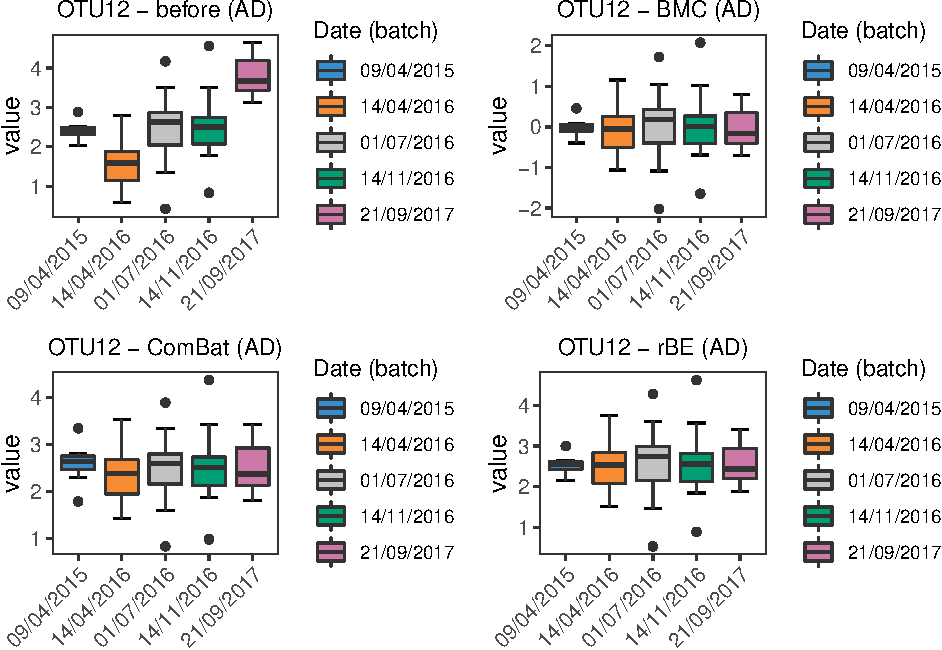
\includegraphics{Managing_batch_effects_files/figure-latex/unnamed-chunk-45-1.pdf}

\begin{Shaded}
\begin{Highlighting}[]
\KeywordTok{grid.arrange}\NormalTok{(sponge.pca.plot.before, sponge.pca.plot.percentile, }
\NormalTok{             sponge.pca.plot.svd, }\DataTypeTok{ncol =} \DecValTok{2}\NormalTok{)}
\end{Highlighting}
\end{Shaded}

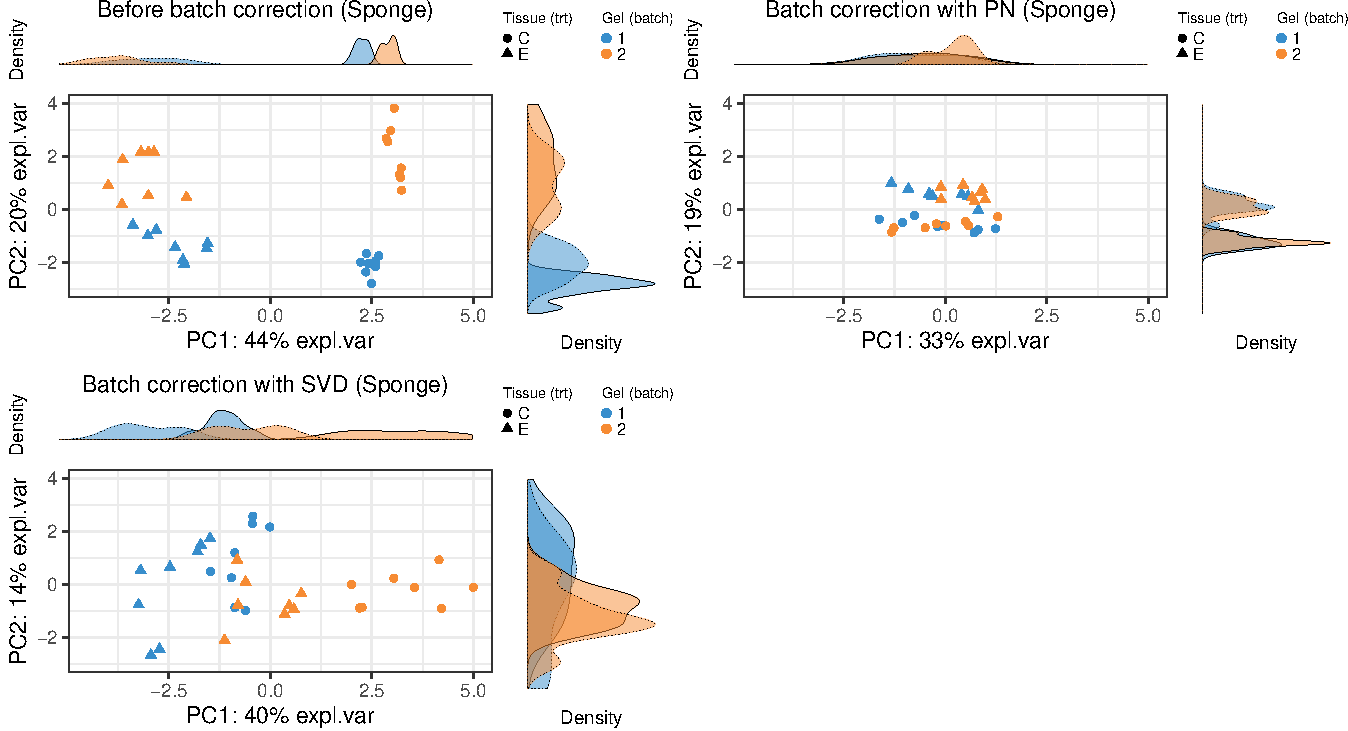
\includegraphics{Managing_batch_effects_files/figure-latex/unnamed-chunk-45-2.pdf}

In sponge data, SVD performed the worse, compared to BMC,
removeBatchEffect and percentile normalisation, as it did not remove
batch effects but removed tissue variation instead.

\begin{Shaded}
\begin{Highlighting}[]
\KeywordTok{grid.arrange}\NormalTok{(ad.pca.plot.before, ad.pca.plot.bmc, }
\NormalTok{             ad.pca.plot.combat, ad.pca.plot.limma, }\DataTypeTok{ncol =} \DecValTok{2}\NormalTok{)}
\end{Highlighting}
\end{Shaded}

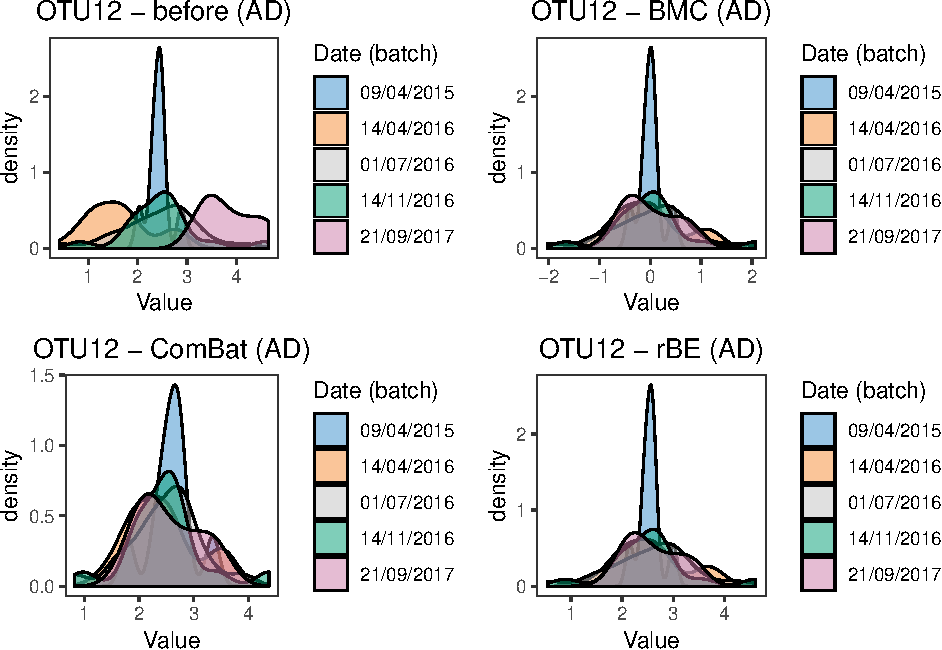
\includegraphics{Managing_batch_effects_files/figure-latex/unnamed-chunk-47-1.pdf}

\begin{Shaded}
\begin{Highlighting}[]
\KeywordTok{grid.arrange}\NormalTok{(ad.pca.plot.before, ad.pca.plot.percentile, }
\NormalTok{             ad.pca.plot.svd, ad.pca.plot.ruv, }\DataTypeTok{ncol =} \DecValTok{2}\NormalTok{)}
\end{Highlighting}
\end{Shaded}

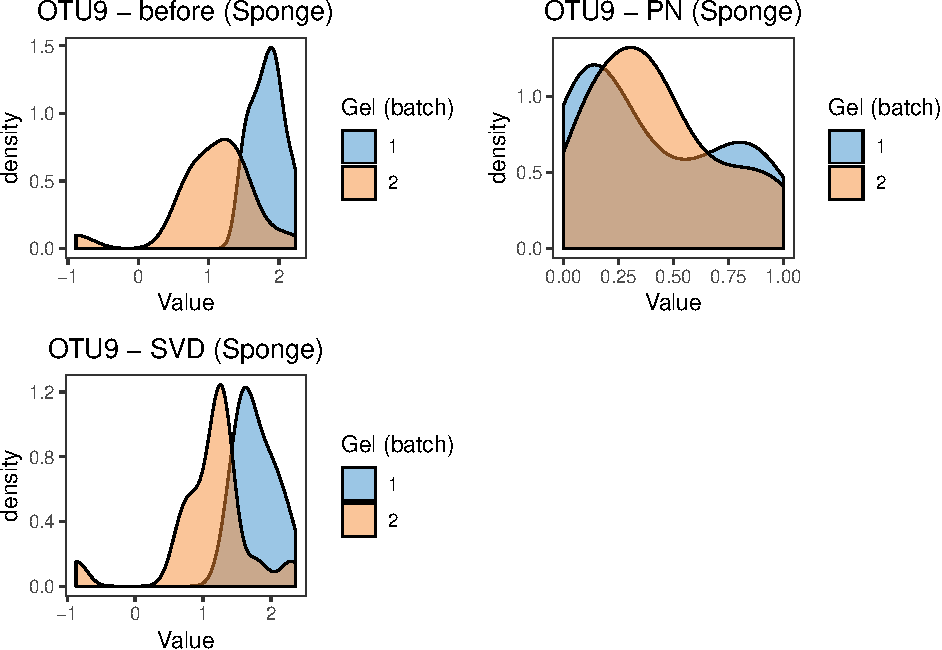
\includegraphics{Managing_batch_effects_files/figure-latex/unnamed-chunk-47-2.pdf}

In AD data, BMC, removeBatchEffect, percentile normalisation and RUVIII
removed the batch effects, and maintained the treatment effects. SVD did
not removed the batch effect but decreased the treatment effects.

\subsection{Density plot and box
plot}\label{density-plot-and-box-plot-1}

\begin{Shaded}
\begin{Highlighting}[]
\CommentTok{# sponge data}
\NormalTok{sponge.before.df <-}\StringTok{ }\KeywordTok{data.frame}\NormalTok{(}\DataTypeTok{value =}\NormalTok{ sponge.tss.clr[ ,}\DecValTok{9}\NormalTok{], }\DataTypeTok{batch =}\NormalTok{ sponge.batch)}
\NormalTok{sponge.boxplot.before <-}\StringTok{ }\KeywordTok{box_plot_fun}\NormalTok{(}\DataTypeTok{data =}\NormalTok{ sponge.before.df, }
                                      \DataTypeTok{x =}\NormalTok{ sponge.before.df}\OperatorTok{$}\NormalTok{batch,}
                                      \DataTypeTok{y =}\NormalTok{ sponge.before.df}\OperatorTok{$}\NormalTok{value, }
                                      \DataTypeTok{title =} \StringTok{'OTU9 - before (Sponge)'}\NormalTok{, }
                                      \DataTypeTok{batch.legend.title =} \StringTok{'Gel (batch)'}\NormalTok{)}

\NormalTok{sponge.bmc.df <-}\StringTok{ }\KeywordTok{data.frame}\NormalTok{(}\DataTypeTok{value =}\NormalTok{ sponge.bmc[ ,}\DecValTok{9}\NormalTok{], }\DataTypeTok{batch =}\NormalTok{ sponge.batch)}
\NormalTok{sponge.boxplot.bmc <-}\StringTok{ }\KeywordTok{box_plot_fun}\NormalTok{(}\DataTypeTok{data =}\NormalTok{ sponge.bmc.df, }
                                   \DataTypeTok{x =}\NormalTok{ sponge.bmc.df}\OperatorTok{$}\NormalTok{batch,}
                                   \DataTypeTok{y =}\NormalTok{ sponge.bmc.df}\OperatorTok{$}\NormalTok{value, }
                                   \DataTypeTok{title =} \StringTok{'OTU9 - BMC (Sponge)'}\NormalTok{, }
                                   \DataTypeTok{batch.legend.title =} \StringTok{'Gel (batch)'}\NormalTok{)}


\NormalTok{sponge.combat.df <-}\StringTok{ }\KeywordTok{data.frame}\NormalTok{(}\DataTypeTok{value =}\NormalTok{ sponge.combat[ ,}\DecValTok{9}\NormalTok{], }\DataTypeTok{batch =}\NormalTok{ sponge.batch)}
\NormalTok{sponge.boxplot.combat <-}\StringTok{ }\KeywordTok{box_plot_fun}\NormalTok{(}\DataTypeTok{data =}\NormalTok{ sponge.combat.df, }
                                      \DataTypeTok{x =}\NormalTok{ sponge.combat.df}\OperatorTok{$}\NormalTok{batch, }
                                      \DataTypeTok{y =}\NormalTok{ sponge.combat.df}\OperatorTok{$}\NormalTok{value, }
                                      \DataTypeTok{title =} \StringTok{'OTU9 - ComBat (Sponge)'}\NormalTok{,}
                                      \DataTypeTok{batch.legend.title =} \StringTok{'Gel (batch)'}\NormalTok{)}


\NormalTok{sponge.limma.df <-}\StringTok{ }\KeywordTok{data.frame}\NormalTok{(}\DataTypeTok{value =}\NormalTok{ sponge.limma[ ,}\DecValTok{9}\NormalTok{], }\DataTypeTok{batch =}\NormalTok{ sponge.batch)}
\NormalTok{sponge.boxplot.limma <-}\StringTok{ }\KeywordTok{box_plot_fun}\NormalTok{(}\DataTypeTok{data =}\NormalTok{ sponge.limma.df, }
                                     \DataTypeTok{x =}\NormalTok{ sponge.limma.df}\OperatorTok{$}\NormalTok{batch, }
                                     \DataTypeTok{y =}\NormalTok{ sponge.limma.df}\OperatorTok{$}\NormalTok{value, }
                                     \DataTypeTok{title =} \StringTok{'OTU9 - rBE(Sponge)'}\NormalTok{, }
                                     \DataTypeTok{batch.legend.title =} \StringTok{'Gel (batch)'}\NormalTok{)}

\NormalTok{sponge.percentile.df <-}\StringTok{ }\KeywordTok{data.frame}\NormalTok{(}\DataTypeTok{value =}\NormalTok{ sponge.percentile[ ,}\DecValTok{9}\NormalTok{], }\DataTypeTok{batch =}\NormalTok{ sponge.batch)}
\NormalTok{sponge.boxplot.percentile <-}\StringTok{ }\KeywordTok{box_plot_fun}\NormalTok{(}\DataTypeTok{data =}\NormalTok{ sponge.percentile.df, }
                                          \DataTypeTok{x =}\NormalTok{ sponge.percentile.df}\OperatorTok{$}\NormalTok{batch, }
                                          \DataTypeTok{y =}\NormalTok{ sponge.percentile.df}\OperatorTok{$}\NormalTok{value, }
                                          \DataTypeTok{title =} \StringTok{'OTU9 - PN (Sponge)'}\NormalTok{, }
                                          \DataTypeTok{batch.legend.title =} \StringTok{'Gel (batch)'}\NormalTok{)}

\NormalTok{sponge.svd.df <-}\StringTok{ }\KeywordTok{data.frame}\NormalTok{(}\DataTypeTok{value =}\NormalTok{ sponge.svd[ ,}\DecValTok{9}\NormalTok{], }\DataTypeTok{batch =}\NormalTok{ sponge.batch)}
\NormalTok{sponge.boxplot.svd <-}\StringTok{ }\KeywordTok{box_plot_fun}\NormalTok{(}\DataTypeTok{data =}\NormalTok{ sponge.svd.df, }
                                   \DataTypeTok{x =}\NormalTok{ sponge.svd.df}\OperatorTok{$}\NormalTok{batch, }
                                   \DataTypeTok{y =}\NormalTok{ sponge.svd.df}\OperatorTok{$}\NormalTok{value, }
                                   \DataTypeTok{title =} \StringTok{'OTU9 - SVD (Sponge)'}\NormalTok{, }
                                   \DataTypeTok{batch.legend.title =} \StringTok{'Gel (batch)'}\NormalTok{)}
\end{Highlighting}
\end{Shaded}

\begin{Shaded}
\begin{Highlighting}[]
\KeywordTok{grid.arrange}\NormalTok{(sponge.boxplot.before, sponge.boxplot.bmc, }
\NormalTok{             sponge.boxplot.combat, sponge.boxplot.limma, }\DataTypeTok{ncol =} \DecValTok{2}\NormalTok{)}
\end{Highlighting}
\end{Shaded}

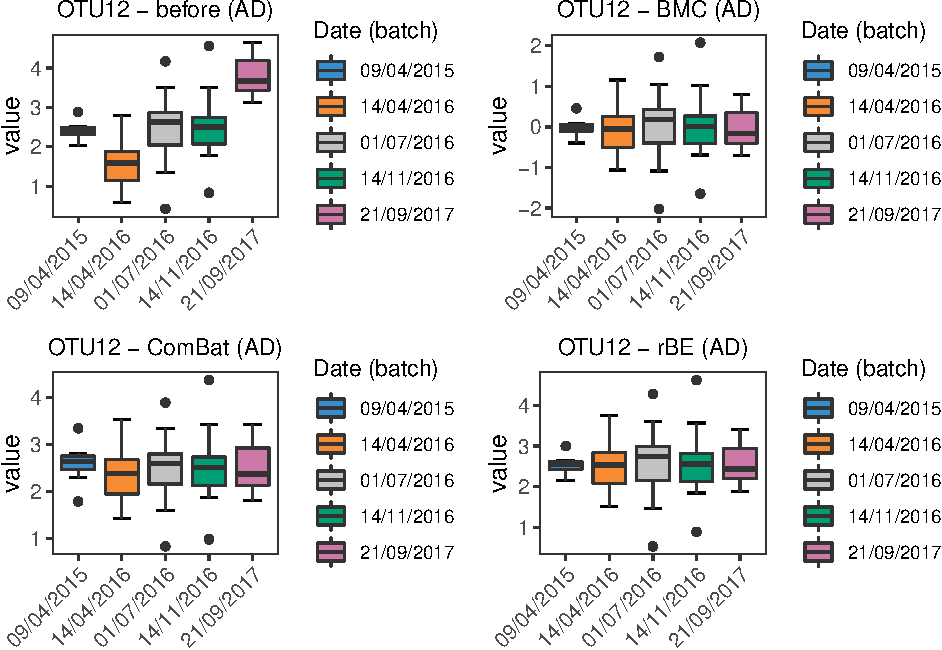
\includegraphics{Managing_batch_effects_files/figure-latex/unnamed-chunk-49-1.pdf}

\begin{Shaded}
\begin{Highlighting}[]
\KeywordTok{grid.arrange}\NormalTok{(sponge.boxplot.before, sponge.boxplot.percentile, }
\NormalTok{             sponge.boxplot.svd, }\DataTypeTok{ncol =} \DecValTok{2}\NormalTok{)}
\end{Highlighting}
\end{Shaded}

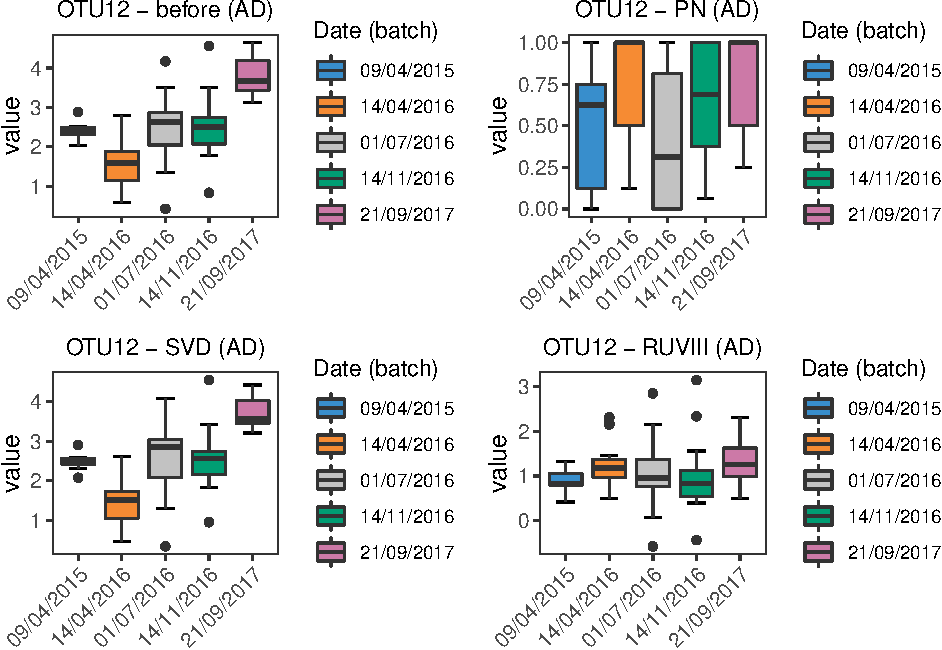
\includegraphics{Managing_batch_effects_files/figure-latex/unnamed-chunk-49-2.pdf}

From the boxplots of OTU9 in sponge data, the difference between two
batches are removed by BMC, ComBat, removeBatchEffect and percentile
normalisation correction. Among these methods, percentile normalisation
does not remove as much batch difference as the other methods.

\begin{Shaded}
\begin{Highlighting}[]
\CommentTok{# density plot}
\CommentTok{# before}
\NormalTok{sponge.dens.before <-}\StringTok{ }\KeywordTok{ggplot}\NormalTok{(sponge.before.df, }\KeywordTok{aes}\NormalTok{(}\DataTypeTok{x =}\NormalTok{ value, }\DataTypeTok{fill =}\NormalTok{ batch)) }\OperatorTok{+}\StringTok{ }
\StringTok{  }\KeywordTok{geom_density}\NormalTok{(}\DataTypeTok{alpha =} \FloatTok{0.5}\NormalTok{) }\OperatorTok{+}\StringTok{ }\KeywordTok{scale_fill_manual}\NormalTok{(}\DataTypeTok{values =} \KeywordTok{color.mixo}\NormalTok{(}\DecValTok{1}\OperatorTok{:}\DecValTok{10}\NormalTok{)) }\OperatorTok{+}\StringTok{ }
\StringTok{  }\KeywordTok{labs}\NormalTok{(}\DataTypeTok{title =} \StringTok{'OTU9 - before (Sponge)'}\NormalTok{, }\DataTypeTok{x =} \StringTok{'Value'}\NormalTok{, }\DataTypeTok{fill =} \StringTok{'Gel (batch)'}\NormalTok{) }\OperatorTok{+}\StringTok{ }
\StringTok{  }\KeywordTok{theme_bw}\NormalTok{() }\OperatorTok{+}\StringTok{ }\KeywordTok{theme}\NormalTok{(}\DataTypeTok{plot.title =} \KeywordTok{element_text}\NormalTok{(}\DataTypeTok{hjust =} \FloatTok{0.5}\NormalTok{), }
                     \DataTypeTok{panel.grid =} \KeywordTok{element_blank}\NormalTok{())}

\CommentTok{# BMC}
\NormalTok{sponge.dens.bmc <-}\StringTok{ }\KeywordTok{ggplot}\NormalTok{(sponge.bmc.df, }\KeywordTok{aes}\NormalTok{(}\DataTypeTok{x =}\NormalTok{ value, }\DataTypeTok{fill =}\NormalTok{ batch)) }\OperatorTok{+}\StringTok{ }
\StringTok{  }\KeywordTok{geom_density}\NormalTok{(}\DataTypeTok{alpha =} \FloatTok{0.5}\NormalTok{) }\OperatorTok{+}\StringTok{ }\KeywordTok{scale_fill_manual}\NormalTok{(}\DataTypeTok{values =} \KeywordTok{color.mixo}\NormalTok{(}\DecValTok{1}\OperatorTok{:}\DecValTok{10}\NormalTok{)) }\OperatorTok{+}\StringTok{ }
\StringTok{  }\KeywordTok{labs}\NormalTok{(}\DataTypeTok{title =} \StringTok{'OTU9 - BMC (Sponge)'}\NormalTok{, }\DataTypeTok{x =} \StringTok{'Value'}\NormalTok{, }\DataTypeTok{fill =} \StringTok{'Gel (batch)'}\NormalTok{) }\OperatorTok{+}\StringTok{ }
\StringTok{  }\KeywordTok{theme_bw}\NormalTok{() }\OperatorTok{+}\StringTok{ }\KeywordTok{theme}\NormalTok{(}\DataTypeTok{plot.title =} \KeywordTok{element_text}\NormalTok{(}\DataTypeTok{hjust =} \FloatTok{0.5}\NormalTok{), }
                     \DataTypeTok{panel.grid =} \KeywordTok{element_blank}\NormalTok{())}


\CommentTok{# ComBat}
\NormalTok{sponge.dens.combat <-}\StringTok{ }\KeywordTok{ggplot}\NormalTok{(sponge.combat.df, }\KeywordTok{aes}\NormalTok{(}\DataTypeTok{x =}\NormalTok{ value, }\DataTypeTok{fill =}\NormalTok{ batch)) }\OperatorTok{+}\StringTok{ }
\StringTok{  }\KeywordTok{geom_density}\NormalTok{(}\DataTypeTok{alpha =} \FloatTok{0.5}\NormalTok{) }\OperatorTok{+}\StringTok{ }\KeywordTok{scale_fill_manual}\NormalTok{(}\DataTypeTok{values =} \KeywordTok{color.mixo}\NormalTok{(}\DecValTok{1}\OperatorTok{:}\DecValTok{10}\NormalTok{)) }\OperatorTok{+}\StringTok{ }
\StringTok{  }\KeywordTok{labs}\NormalTok{(}\DataTypeTok{title =} \StringTok{'OTU9 - ComBat (Sponge)'}\NormalTok{, }\DataTypeTok{x =} \StringTok{'Value'}\NormalTok{, }\DataTypeTok{fill =} \StringTok{'Gel (batch)'}\NormalTok{) }\OperatorTok{+}\StringTok{ }
\StringTok{  }\KeywordTok{theme_bw}\NormalTok{() }\OperatorTok{+}\StringTok{ }\KeywordTok{theme}\NormalTok{(}\DataTypeTok{plot.title =} \KeywordTok{element_text}\NormalTok{(}\DataTypeTok{hjust =} \FloatTok{0.5}\NormalTok{), }
                     \DataTypeTok{panel.grid =} \KeywordTok{element_blank}\NormalTok{())}


\CommentTok{# removeBatchEffect }
\NormalTok{sponge.dens.limma <-}\StringTok{ }\KeywordTok{ggplot}\NormalTok{(sponge.limma.df, }\KeywordTok{aes}\NormalTok{(}\DataTypeTok{x =}\NormalTok{ value, }\DataTypeTok{fill =}\NormalTok{ batch)) }\OperatorTok{+}\StringTok{ }
\StringTok{  }\KeywordTok{geom_density}\NormalTok{(}\DataTypeTok{alpha =} \FloatTok{0.5}\NormalTok{) }\OperatorTok{+}\StringTok{ }\KeywordTok{scale_fill_manual}\NormalTok{(}\DataTypeTok{values =} \KeywordTok{color.mixo}\NormalTok{(}\DecValTok{1}\OperatorTok{:}\DecValTok{10}\NormalTok{)) }\OperatorTok{+}\StringTok{ }
\StringTok{  }\KeywordTok{labs}\NormalTok{(}\DataTypeTok{title =} \StringTok{'OTU9 - rBE (Sponge)'}\NormalTok{, }\DataTypeTok{x =} \StringTok{'Value'}\NormalTok{, }\DataTypeTok{fill =} \StringTok{'Gel (batch)'}\NormalTok{) }\OperatorTok{+}\StringTok{ }
\StringTok{  }\KeywordTok{theme_bw}\NormalTok{() }\OperatorTok{+}\StringTok{ }\KeywordTok{theme}\NormalTok{(}\DataTypeTok{plot.title =} \KeywordTok{element_text}\NormalTok{(}\DataTypeTok{hjust =} \FloatTok{0.5}\NormalTok{), }
                     \DataTypeTok{panel.grid =} \KeywordTok{element_blank}\NormalTok{())}


\CommentTok{# percentile normal}
\NormalTok{sponge.dens.percentile <-}\StringTok{ }\KeywordTok{ggplot}\NormalTok{(sponge.percentile.df, }\KeywordTok{aes}\NormalTok{(}\DataTypeTok{x =}\NormalTok{ value, }\DataTypeTok{fill =}\NormalTok{ batch)) }\OperatorTok{+}\StringTok{ }
\StringTok{  }\KeywordTok{geom_density}\NormalTok{(}\DataTypeTok{alpha =} \FloatTok{0.5}\NormalTok{) }\OperatorTok{+}\StringTok{ }\KeywordTok{scale_fill_manual}\NormalTok{(}\DataTypeTok{values =} \KeywordTok{color.mixo}\NormalTok{(}\DecValTok{1}\OperatorTok{:}\DecValTok{10}\NormalTok{)) }\OperatorTok{+}\StringTok{ }
\StringTok{  }\KeywordTok{labs}\NormalTok{(}\DataTypeTok{title =} \StringTok{'OTU9 - PN (Sponge)'}\NormalTok{, }\DataTypeTok{x =} \StringTok{'Value'}\NormalTok{, }\DataTypeTok{fill =} \StringTok{'Gel (batch)'}\NormalTok{) }\OperatorTok{+}\StringTok{ }
\StringTok{  }\KeywordTok{theme_bw}\NormalTok{() }\OperatorTok{+}\StringTok{ }\KeywordTok{theme}\NormalTok{(}\DataTypeTok{plot.title =} \KeywordTok{element_text}\NormalTok{(}\DataTypeTok{hjust =} \FloatTok{0.5}\NormalTok{), }
                     \DataTypeTok{panel.grid =} \KeywordTok{element_blank}\NormalTok{())}


\CommentTok{# SVD}
\NormalTok{sponge.dens.svd <-}\StringTok{ }\KeywordTok{ggplot}\NormalTok{(sponge.svd.df, }\KeywordTok{aes}\NormalTok{(}\DataTypeTok{x =}\NormalTok{ value, }\DataTypeTok{fill =}\NormalTok{ batch)) }\OperatorTok{+}\StringTok{ }
\StringTok{  }\KeywordTok{geom_density}\NormalTok{(}\DataTypeTok{alpha =} \FloatTok{0.5}\NormalTok{) }\OperatorTok{+}\StringTok{ }\KeywordTok{scale_fill_manual}\NormalTok{(}\DataTypeTok{values =} \KeywordTok{color.mixo}\NormalTok{(}\DecValTok{1}\OperatorTok{:}\DecValTok{10}\NormalTok{)) }\OperatorTok{+}\StringTok{ }
\StringTok{  }\KeywordTok{labs}\NormalTok{(}\DataTypeTok{title =} \StringTok{'OTU9 - SVD (Sponge)'}\NormalTok{, }\DataTypeTok{x =} \StringTok{'Value'}\NormalTok{, }\DataTypeTok{fill =} \StringTok{'Gel (batch)'}\NormalTok{) }\OperatorTok{+}\StringTok{ }
\StringTok{  }\KeywordTok{theme_bw}\NormalTok{() }\OperatorTok{+}\StringTok{ }\KeywordTok{theme}\NormalTok{(}\DataTypeTok{plot.title =} \KeywordTok{element_text}\NormalTok{(}\DataTypeTok{hjust =} \FloatTok{0.5}\NormalTok{), }
                     \DataTypeTok{panel.grid =} \KeywordTok{element_blank}\NormalTok{())}
\end{Highlighting}
\end{Shaded}

\begin{Shaded}
\begin{Highlighting}[]
\KeywordTok{grid.arrange}\NormalTok{(sponge.dens.before, sponge.dens.bmc, }
\NormalTok{             sponge.dens.combat, sponge.dens.limma, }\DataTypeTok{ncol =} \DecValTok{2}\NormalTok{)}
\end{Highlighting}
\end{Shaded}

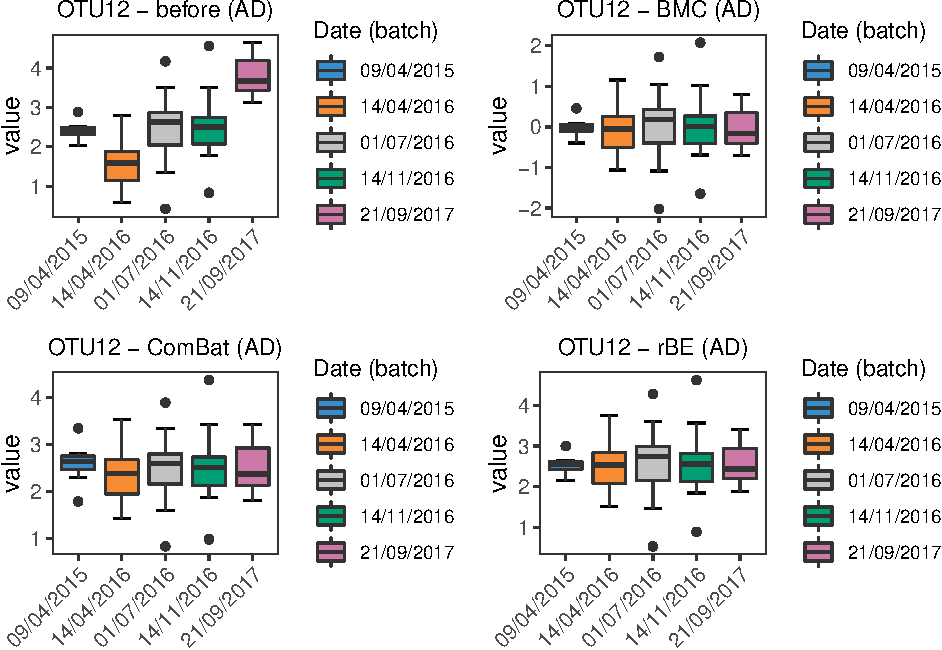
\includegraphics{Managing_batch_effects_files/figure-latex/unnamed-chunk-51-1.pdf}

\begin{Shaded}
\begin{Highlighting}[]
\KeywordTok{grid.arrange}\NormalTok{(sponge.dens.before, sponge.dens.percentile, }
\NormalTok{             sponge.dens.svd, }\DataTypeTok{ncol =} \DecValTok{2}\NormalTok{)}
\end{Highlighting}
\end{Shaded}

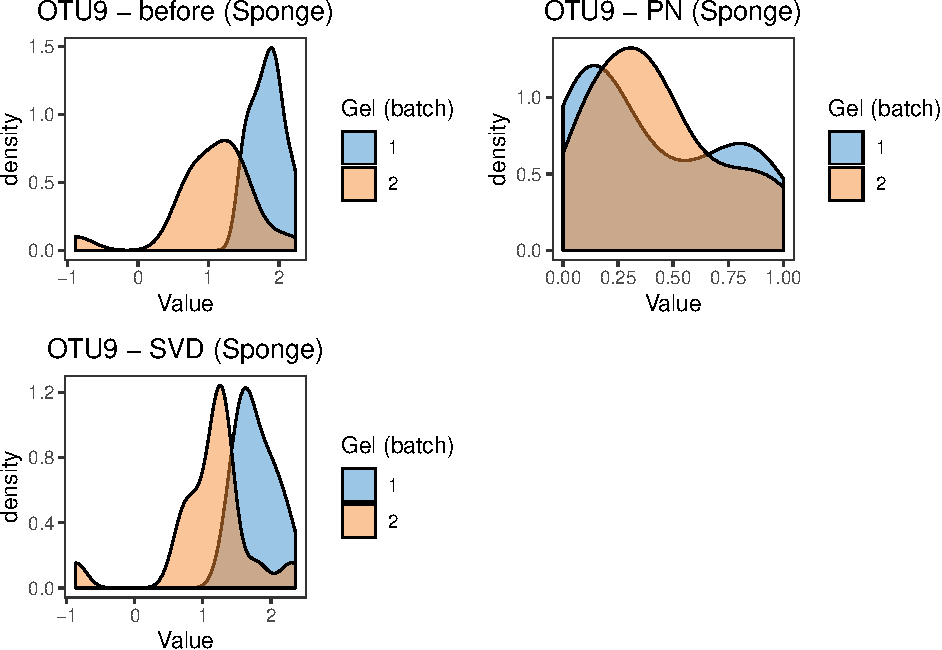
\includegraphics{Managing_batch_effects_files/figure-latex/unnamed-chunk-51-2.pdf}

We can also assess the effect of batch in a linear model before and
after batch correction.

\begin{Shaded}
\begin{Highlighting}[]
\CommentTok{# P-values}
\NormalTok{sponge.lm.before <-}\StringTok{ }\KeywordTok{lm}\NormalTok{(sponge.tss.clr[ ,}\DecValTok{9}\NormalTok{] }\OperatorTok{~}\StringTok{ }\NormalTok{sponge.trt }\OperatorTok{+}\StringTok{ }\NormalTok{sponge.batch)}
\KeywordTok{summary}\NormalTok{(sponge.lm.before)}
\end{Highlighting}
\end{Shaded}

\begin{verbatim}
## 
## Call:
## lm(formula = sponge.tss.clr[, 9] ~ sponge.trt + sponge.batch)
## 
## Residuals:
##      Min       1Q   Median       3Q      Max 
## -1.87967 -0.24705  0.04588  0.24492  1.00757 
## 
## Coefficients:
##               Estimate Std. Error t value Pr(>|t|)    
## (Intercept)     1.7849     0.1497  11.922 1.06e-12 ***
## sponge.trtE     0.1065     0.1729   0.616    0.543    
## sponge.batch2  -0.7910     0.1729  -4.575 8.24e-05 ***
## ---
## Signif. codes:  0 '***' 0.001 '**' 0.01 '*' 0.05 '.' 0.1 ' ' 1
## 
## Residual standard error: 0.489 on 29 degrees of freedom
## Multiple R-squared:  0.4236, Adjusted R-squared:  0.3839 
## F-statistic: 10.66 on 2 and 29 DF,  p-value: 0.0003391
\end{verbatim}

Before correction, the batch effect is statistically significant (P
\(<\) 0.001), as indicated in the \textbf{sponge.batch2} row.

\begin{Shaded}
\begin{Highlighting}[]
\NormalTok{sponge.lm.bmc <-}\StringTok{ }\KeywordTok{lm}\NormalTok{(sponge.bmc[ ,}\DecValTok{9}\NormalTok{] }\OperatorTok{~}\StringTok{ }\NormalTok{sponge.trt }\OperatorTok{+}\StringTok{ }\NormalTok{sponge.batch)}
\KeywordTok{summary}\NormalTok{(sponge.lm.bmc)}
\end{Highlighting}
\end{Shaded}

\begin{verbatim}
## 
## Call:
## lm(formula = sponge.bmc[, 9] ~ sponge.trt + sponge.batch)
## 
## Residuals:
##      Min       1Q   Median       3Q      Max 
## -1.87967 -0.24705  0.04588  0.24492  1.00757 
## 
## Coefficients:
##                 Estimate Std. Error t value Pr(>|t|)
## (Intercept)   -5.323e-02  1.497e-01  -0.356    0.725
## sponge.trtE    1.065e-01  1.729e-01   0.616    0.543
## sponge.batch2 -3.925e-17  1.729e-01   0.000    1.000
## 
## Residual standard error: 0.489 on 29 degrees of freedom
## Multiple R-squared:  0.01291,    Adjusted R-squared:  -0.05517 
## F-statistic: 0.1896 on 2 and 29 DF,  p-value: 0.8283
\end{verbatim}

After BMC correction, the batch effect is not statistically significant
(P \(>\) 0.05), as indicated in the \textbf{sponge.batch2} row.

The results from other batch correction methods are similar as BMC
correction.

\begin{Shaded}
\begin{Highlighting}[]
\NormalTok{sponge.lm.combat <-}\StringTok{ }\KeywordTok{lm}\NormalTok{(sponge.combat[ ,}\DecValTok{9}\NormalTok{] }\OperatorTok{~}\StringTok{ }\NormalTok{sponge.trt }\OperatorTok{+}\StringTok{ }\NormalTok{sponge.batch)}
\KeywordTok{summary}\NormalTok{(sponge.lm.combat)}

\NormalTok{sponge.lm.limma <-}\StringTok{ }\KeywordTok{lm}\NormalTok{(sponge.limma[ ,}\DecValTok{9}\NormalTok{] }\OperatorTok{~}\StringTok{ }\NormalTok{sponge.trt }\OperatorTok{+}\StringTok{ }\NormalTok{sponge.batch)}
\KeywordTok{summary}\NormalTok{(sponge.lm.limma)}

\NormalTok{sponge.lm.percentile <-}\StringTok{ }\KeywordTok{lm}\NormalTok{(sponge.percentile[ ,}\DecValTok{9}\NormalTok{] }\OperatorTok{~}\StringTok{ }\NormalTok{sponge.trt }\OperatorTok{+}\StringTok{ }\NormalTok{sponge.batch)}
\KeywordTok{summary}\NormalTok{(sponge.lm.percentile)}

\NormalTok{sponge.lm.svd <-}\StringTok{ }\KeywordTok{lm}\NormalTok{(sponge.svd[ ,}\DecValTok{9}\NormalTok{] }\OperatorTok{~}\StringTok{ }\NormalTok{sponge.trt }\OperatorTok{+}\StringTok{ }\NormalTok{sponge.batch)}
\KeywordTok{summary}\NormalTok{(sponge.lm.svd)}
\end{Highlighting}
\end{Shaded}

In sponge data, the results of density plots and P-values of batch
effects from linear models reach a consesus with boxplots, the
difference between two batches are removed by BMC, ComBat,
removeBatchEffect and percentile normalisation correction. We observe
that percentile normalisation modifies the distribution of the samples
from the two batches.

\begin{Shaded}
\begin{Highlighting}[]
\CommentTok{# ad data}
\CommentTok{# boxplot}
\NormalTok{ad.before.df <-}\StringTok{ }\KeywordTok{data.frame}\NormalTok{(}\DataTypeTok{value =}\NormalTok{ ad.clr[ ,}\DecValTok{1}\NormalTok{], }\DataTypeTok{batch =}\NormalTok{ ad.batch)}
\NormalTok{ad.boxplot.before <-}\StringTok{ }\KeywordTok{box_plot_fun}\NormalTok{(}\DataTypeTok{data =}\NormalTok{ ad.before.df, }\DataTypeTok{x =}\NormalTok{ ad.before.df}\OperatorTok{$}\NormalTok{batch, }
                                  \DataTypeTok{y =}\NormalTok{ ad.before.df}\OperatorTok{$}\NormalTok{value, }
                                  \DataTypeTok{title =} \StringTok{'OTU12 - before (AD)'}\NormalTok{, }
                                  \DataTypeTok{batch.legend.title =} \StringTok{'Date (batch)'}\NormalTok{, }
                                  \DataTypeTok{x.angle =} \DecValTok{45}\NormalTok{, }\DataTypeTok{x.hjust =} \DecValTok{1}\NormalTok{)}


\NormalTok{ad.bmc.df <-}\StringTok{ }\KeywordTok{data.frame}\NormalTok{(}\DataTypeTok{value =}\NormalTok{ ad.bmc[ ,}\DecValTok{1}\NormalTok{], }\DataTypeTok{batch =}\NormalTok{ ad.batch)}
\NormalTok{ad.boxplot.bmc <-}\StringTok{ }\KeywordTok{box_plot_fun}\NormalTok{(}\DataTypeTok{data =}\NormalTok{ ad.bmc.df,}\DataTypeTok{x =}\NormalTok{ ad.bmc.df}\OperatorTok{$}\NormalTok{batch, }
                               \DataTypeTok{y =}\NormalTok{ ad.bmc.df}\OperatorTok{$}\NormalTok{value, }
                               \DataTypeTok{title =} \StringTok{'OTU12 - BMC (AD)'}\NormalTok{, }
                               \DataTypeTok{batch.legend.title =} \StringTok{'Date (batch)'}\NormalTok{, }
                               \DataTypeTok{x.angle =} \DecValTok{45}\NormalTok{, }\DataTypeTok{x.hjust =} \DecValTok{1}\NormalTok{)}


\NormalTok{ad.combat.df <-}\StringTok{ }\KeywordTok{data.frame}\NormalTok{(}\DataTypeTok{value =}\NormalTok{ ad.combat[ ,}\DecValTok{1}\NormalTok{], }\DataTypeTok{batch =}\NormalTok{ ad.batch)}
\NormalTok{ad.boxplot.combat <-}\StringTok{ }\KeywordTok{box_plot_fun}\NormalTok{(}\DataTypeTok{data =}\NormalTok{ ad.combat.df, }\DataTypeTok{x =}\NormalTok{ ad.combat.df}\OperatorTok{$}\NormalTok{batch,}
                                  \DataTypeTok{y =}\NormalTok{ ad.combat.df}\OperatorTok{$}\NormalTok{value, }
                                  \DataTypeTok{title =} \StringTok{'OTU12 - ComBat (AD)'}\NormalTok{, }
                                  \DataTypeTok{batch.legend.title =} \StringTok{'Date (batch)'}\NormalTok{, }
                                  \DataTypeTok{x.angle =} \DecValTok{45}\NormalTok{, }\DataTypeTok{x.hjust =} \DecValTok{1}\NormalTok{)}

\NormalTok{ad.limma.df <-}\StringTok{ }\KeywordTok{data.frame}\NormalTok{(}\DataTypeTok{value =}\NormalTok{ ad.limma[ ,}\DecValTok{1}\NormalTok{], }\DataTypeTok{batch =}\NormalTok{ ad.batch)}
\NormalTok{ad.boxplot.limma <-}\StringTok{ }\KeywordTok{box_plot_fun}\NormalTok{(}\DataTypeTok{data =}\NormalTok{ ad.limma.df,}\DataTypeTok{x =}\NormalTok{ ad.limma.df}\OperatorTok{$}\NormalTok{batch, }
                                 \DataTypeTok{y =}\NormalTok{ ad.limma.df}\OperatorTok{$}\NormalTok{value, }
                                 \DataTypeTok{title =} \StringTok{'OTU12 - rBE (AD)'}\NormalTok{, }
                                 \DataTypeTok{batch.legend.title =} \StringTok{'Date (batch)'}\NormalTok{, }
                                 \DataTypeTok{x.angle =} \DecValTok{45}\NormalTok{, }\DataTypeTok{x.hjust =} \DecValTok{1}\NormalTok{)}


\NormalTok{ad.percentile.df <-}\StringTok{ }\KeywordTok{data.frame}\NormalTok{(}\DataTypeTok{value =}\NormalTok{ ad.percentile[ ,}\DecValTok{1}\NormalTok{], }\DataTypeTok{batch =}\NormalTok{ ad.batch)}
\NormalTok{ad.boxplot.percentile <-}\StringTok{ }\KeywordTok{box_plot_fun}\NormalTok{(}\DataTypeTok{data =}\NormalTok{ ad.percentile.df,}\DataTypeTok{x =}\NormalTok{ ad.percentile.df}\OperatorTok{$}\NormalTok{batch, }
                                      \DataTypeTok{y =}\NormalTok{ ad.percentile.df}\OperatorTok{$}\NormalTok{value, }
                                      \DataTypeTok{title =} \StringTok{'OTU12 - PN (AD)'}\NormalTok{, }
                                      \DataTypeTok{batch.legend.title =} \StringTok{'Date (batch)'}\NormalTok{, }
                                      \DataTypeTok{x.angle =} \DecValTok{45}\NormalTok{, }\DataTypeTok{x.hjust =} \DecValTok{1}\NormalTok{)}

\NormalTok{ad.svd.df <-}\StringTok{ }\KeywordTok{data.frame}\NormalTok{(}\DataTypeTok{value =}\NormalTok{ ad.svd[ ,}\DecValTok{1}\NormalTok{], }\DataTypeTok{batch =}\NormalTok{ ad.batch)}
\NormalTok{ad.boxplot.svd <-}\StringTok{ }\KeywordTok{box_plot_fun}\NormalTok{(}\DataTypeTok{data =}\NormalTok{ ad.svd.df,}\DataTypeTok{x =}\NormalTok{ ad.svd.df}\OperatorTok{$}\NormalTok{batch, }
                               \DataTypeTok{y =}\NormalTok{ ad.svd.df}\OperatorTok{$}\NormalTok{value, }
                               \DataTypeTok{title =} \StringTok{'OTU12 - SVD (AD)'}\NormalTok{, }
                               \DataTypeTok{batch.legend.title =} \StringTok{'Date (batch)'}\NormalTok{, }
                               \DataTypeTok{x.angle =} \DecValTok{45}\NormalTok{, }\DataTypeTok{x.hjust =} \DecValTok{1}\NormalTok{)}

\NormalTok{ad.ruv.df <-}\StringTok{ }\KeywordTok{data.frame}\NormalTok{(}\DataTypeTok{value =}\NormalTok{ ad.ruvIII[ ,}\DecValTok{1}\NormalTok{], }\DataTypeTok{batch =}\NormalTok{ ad.batch)}
\NormalTok{ad.boxplot.ruv <-}\StringTok{ }\KeywordTok{box_plot_fun}\NormalTok{(}\DataTypeTok{data =}\NormalTok{ ad.ruv.df,}\DataTypeTok{x =}\NormalTok{ ad.ruv.df}\OperatorTok{$}\NormalTok{batch, }
                               \DataTypeTok{y =}\NormalTok{ ad.ruv.df}\OperatorTok{$}\NormalTok{value, }
                               \DataTypeTok{title =} \StringTok{'OTU12 - RUVIII (AD)'}\NormalTok{, }
                               \DataTypeTok{batch.legend.title =} \StringTok{'Date (batch)'}\NormalTok{, }
                               \DataTypeTok{x.angle =} \DecValTok{45}\NormalTok{, }\DataTypeTok{x.hjust =} \DecValTok{1}\NormalTok{)}
\end{Highlighting}
\end{Shaded}

\begin{Shaded}
\begin{Highlighting}[]
\KeywordTok{grid.arrange}\NormalTok{(ad.boxplot.before, ad.boxplot.bmc, }
\NormalTok{             ad.boxplot.combat, ad.boxplot.limma, }\DataTypeTok{ncol =} \DecValTok{2}\NormalTok{)}
\end{Highlighting}
\end{Shaded}

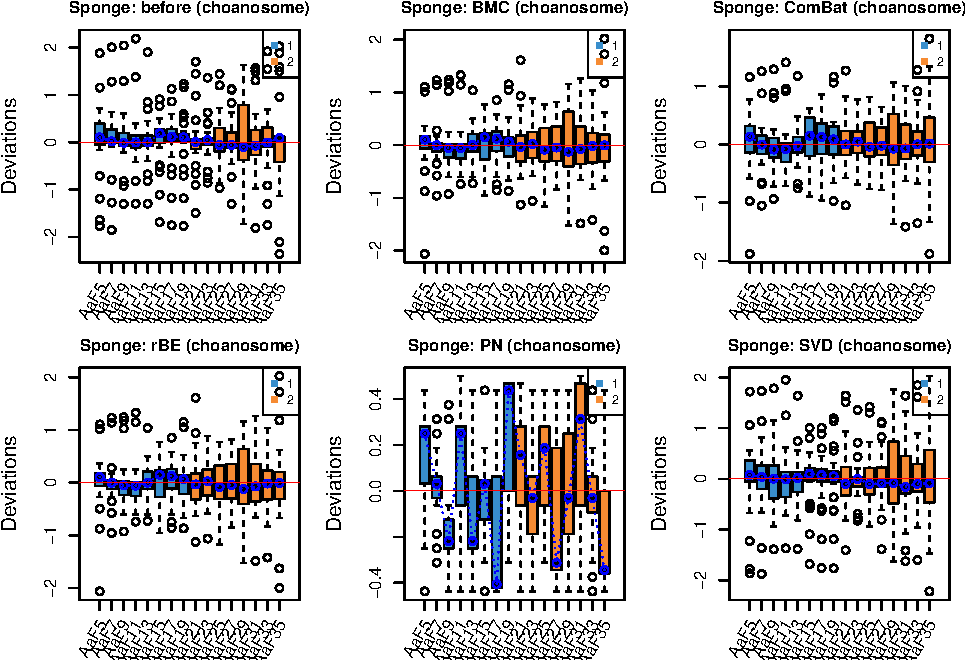
\includegraphics{Managing_batch_effects_files/figure-latex/unnamed-chunk-56-1.pdf}

\begin{Shaded}
\begin{Highlighting}[]
\KeywordTok{grid.arrange}\NormalTok{(ad.boxplot.before, ad.boxplot.percentile, }
\NormalTok{             ad.boxplot.svd, ad.boxplot.ruv, }\DataTypeTok{ncol =} \DecValTok{2}\NormalTok{)}
\end{Highlighting}
\end{Shaded}

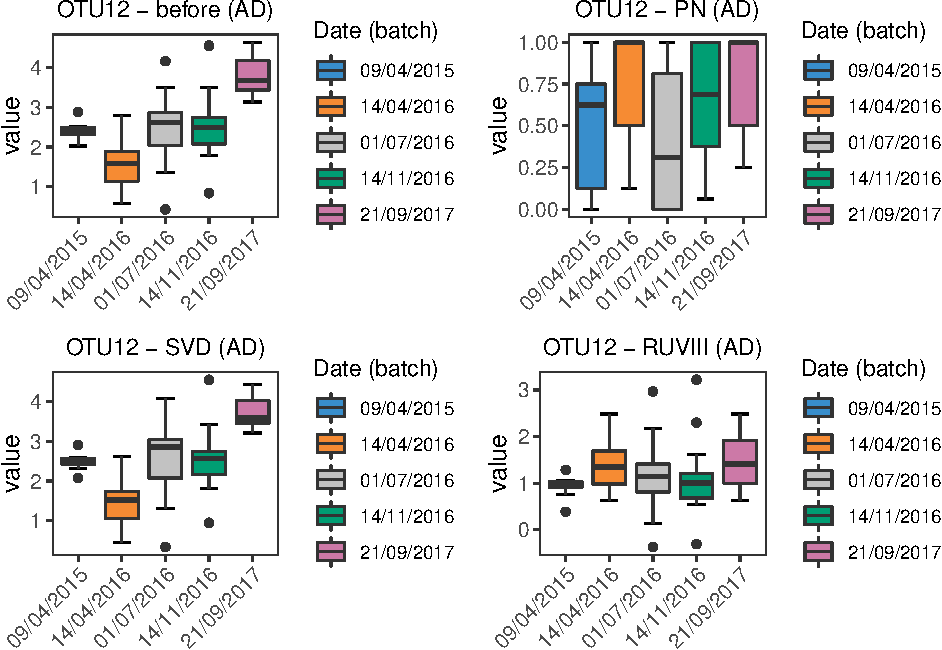
\includegraphics{Managing_batch_effects_files/figure-latex/unnamed-chunk-56-2.pdf}

From the boxplots of OTU9 in AD data, the difference between five
batches are removed by BMC, ComBat, removeBatchEffect and RUVIII
correction. Among these methods, RUVIII did not remove as much batch
difference as the other methods.

\begin{Shaded}
\begin{Highlighting}[]
\CommentTok{# density plot}
\CommentTok{# before}
\NormalTok{ad.dens.before <-}\StringTok{ }\KeywordTok{ggplot}\NormalTok{(ad.before.df, }\KeywordTok{aes}\NormalTok{(}\DataTypeTok{x =}\NormalTok{ value, }\DataTypeTok{fill =}\NormalTok{ batch)) }\OperatorTok{+}\StringTok{ }
\StringTok{  }\KeywordTok{geom_density}\NormalTok{(}\DataTypeTok{alpha =} \FloatTok{0.5}\NormalTok{) }\OperatorTok{+}\StringTok{ }\KeywordTok{scale_fill_manual}\NormalTok{(}\DataTypeTok{values =} \KeywordTok{color.mixo}\NormalTok{(}\DecValTok{1}\OperatorTok{:}\DecValTok{10}\NormalTok{)) }\OperatorTok{+}\StringTok{ }
\StringTok{  }\KeywordTok{labs}\NormalTok{(}\DataTypeTok{title =} \StringTok{'OTU12 - before (AD)'}\NormalTok{, }\DataTypeTok{x =} \StringTok{'Value'}\NormalTok{, }\DataTypeTok{fill =} \StringTok{'Date (batch)'}\NormalTok{) }\OperatorTok{+}\StringTok{ }
\StringTok{  }\KeywordTok{theme_bw}\NormalTok{() }\OperatorTok{+}\StringTok{ }\KeywordTok{theme}\NormalTok{(}\DataTypeTok{plot.title =} \KeywordTok{element_text}\NormalTok{(}\DataTypeTok{hjust =} \FloatTok{0.5}\NormalTok{), }
                     \DataTypeTok{panel.grid =} \KeywordTok{element_blank}\NormalTok{())}

\CommentTok{# BMC}
\NormalTok{ad.dens.bmc <-}\StringTok{ }\KeywordTok{ggplot}\NormalTok{(ad.bmc.df, }\KeywordTok{aes}\NormalTok{(}\DataTypeTok{x =}\NormalTok{ value, }\DataTypeTok{fill =}\NormalTok{ batch)) }\OperatorTok{+}\StringTok{ }
\StringTok{  }\KeywordTok{geom_density}\NormalTok{(}\DataTypeTok{alpha =} \FloatTok{0.5}\NormalTok{) }\OperatorTok{+}\StringTok{ }\KeywordTok{scale_fill_manual}\NormalTok{(}\DataTypeTok{values =} \KeywordTok{color.mixo}\NormalTok{(}\DecValTok{1}\OperatorTok{:}\DecValTok{10}\NormalTok{)) }\OperatorTok{+}\StringTok{ }
\StringTok{  }\KeywordTok{labs}\NormalTok{(}\DataTypeTok{title =} \StringTok{'OTU12 - BMC (AD)'}\NormalTok{, }\DataTypeTok{x =} \StringTok{'Value'}\NormalTok{, }\DataTypeTok{fill =} \StringTok{'Date (batch)'}\NormalTok{) }\OperatorTok{+}\StringTok{ }
\StringTok{  }\KeywordTok{theme_bw}\NormalTok{() }\OperatorTok{+}\StringTok{ }\KeywordTok{theme}\NormalTok{(}\DataTypeTok{plot.title =} \KeywordTok{element_text}\NormalTok{(}\DataTypeTok{hjust =} \FloatTok{0.5}\NormalTok{), }
                     \DataTypeTok{panel.grid =} \KeywordTok{element_blank}\NormalTok{())}


\CommentTok{# ComBat}
\NormalTok{ad.dens.combat <-}\StringTok{ }\KeywordTok{ggplot}\NormalTok{(ad.combat.df, }\KeywordTok{aes}\NormalTok{(}\DataTypeTok{x =}\NormalTok{ value, }\DataTypeTok{fill =}\NormalTok{ batch)) }\OperatorTok{+}\StringTok{ }
\StringTok{  }\KeywordTok{geom_density}\NormalTok{(}\DataTypeTok{alpha =} \FloatTok{0.5}\NormalTok{) }\OperatorTok{+}\StringTok{ }\KeywordTok{scale_fill_manual}\NormalTok{(}\DataTypeTok{values =} \KeywordTok{color.mixo}\NormalTok{(}\DecValTok{1}\OperatorTok{:}\DecValTok{10}\NormalTok{)) }\OperatorTok{+}\StringTok{ }
\StringTok{  }\KeywordTok{labs}\NormalTok{(}\DataTypeTok{title =} \StringTok{'OTU12 - ComBat (AD)'}\NormalTok{, }\DataTypeTok{x =} \StringTok{'Value'}\NormalTok{, }\DataTypeTok{fill =} \StringTok{'Date (batch)'}\NormalTok{) }\OperatorTok{+}\StringTok{ }
\StringTok{  }\KeywordTok{theme_bw}\NormalTok{() }\OperatorTok{+}\StringTok{ }\KeywordTok{theme}\NormalTok{(}\DataTypeTok{plot.title =} \KeywordTok{element_text}\NormalTok{(}\DataTypeTok{hjust =} \FloatTok{0.5}\NormalTok{), }
                     \DataTypeTok{panel.grid =} \KeywordTok{element_blank}\NormalTok{())}


\CommentTok{# removeBatchEffect}
\NormalTok{ad.dens.limma <-}\StringTok{ }\KeywordTok{ggplot}\NormalTok{(ad.limma.df, }\KeywordTok{aes}\NormalTok{(}\DataTypeTok{x =}\NormalTok{ value, }\DataTypeTok{fill =}\NormalTok{ batch)) }\OperatorTok{+}\StringTok{ }
\StringTok{  }\KeywordTok{geom_density}\NormalTok{(}\DataTypeTok{alpha =} \FloatTok{0.5}\NormalTok{) }\OperatorTok{+}\StringTok{ }\KeywordTok{scale_fill_manual}\NormalTok{(}\DataTypeTok{values =} \KeywordTok{color.mixo}\NormalTok{(}\DecValTok{1}\OperatorTok{:}\DecValTok{10}\NormalTok{)) }\OperatorTok{+}\StringTok{ }
\StringTok{  }\KeywordTok{labs}\NormalTok{(}\DataTypeTok{title =} \StringTok{'OTU12 - rBE (AD)'}\NormalTok{, }\DataTypeTok{x =} \StringTok{'Value'}\NormalTok{, }\DataTypeTok{fill =} \StringTok{'Date (batch)'}\NormalTok{) }\OperatorTok{+}\StringTok{ }
\StringTok{  }\KeywordTok{theme_bw}\NormalTok{() }\OperatorTok{+}\StringTok{ }\KeywordTok{theme}\NormalTok{(}\DataTypeTok{plot.title =} \KeywordTok{element_text}\NormalTok{(}\DataTypeTok{hjust =} \FloatTok{0.5}\NormalTok{), }
                     \DataTypeTok{panel.grid =} \KeywordTok{element_blank}\NormalTok{())}


\CommentTok{# percentile norm}
\NormalTok{ad.dens.percentile <-}\StringTok{ }\KeywordTok{ggplot}\NormalTok{(ad.percentile.df, }\KeywordTok{aes}\NormalTok{(}\DataTypeTok{x =}\NormalTok{ value, }\DataTypeTok{fill =}\NormalTok{ batch)) }\OperatorTok{+}\StringTok{ }
\StringTok{  }\KeywordTok{geom_density}\NormalTok{(}\DataTypeTok{alpha =} \FloatTok{0.5}\NormalTok{) }\OperatorTok{+}\StringTok{ }\KeywordTok{scale_fill_manual}\NormalTok{(}\DataTypeTok{values =} \KeywordTok{color.mixo}\NormalTok{(}\DecValTok{1}\OperatorTok{:}\DecValTok{10}\NormalTok{)) }\OperatorTok{+}\StringTok{ }
\StringTok{  }\KeywordTok{labs}\NormalTok{(}\DataTypeTok{title =} \StringTok{'OTU12 - PN (AD)'}\NormalTok{, }\DataTypeTok{x =} \StringTok{'Value'}\NormalTok{, }\DataTypeTok{fill =} \StringTok{'Date (batch)'}\NormalTok{) }\OperatorTok{+}\StringTok{ }
\StringTok{  }\KeywordTok{theme_bw}\NormalTok{() }\OperatorTok{+}\StringTok{ }\KeywordTok{theme}\NormalTok{(}\DataTypeTok{plot.title =} \KeywordTok{element_text}\NormalTok{(}\DataTypeTok{hjust =} \FloatTok{0.5}\NormalTok{), }
                     \DataTypeTok{panel.grid =} \KeywordTok{element_blank}\NormalTok{())}


\CommentTok{# SVD}
\NormalTok{ad.dens.svd <-}\StringTok{ }\KeywordTok{ggplot}\NormalTok{(ad.svd.df, }\KeywordTok{aes}\NormalTok{(}\DataTypeTok{x =}\NormalTok{ value, }\DataTypeTok{fill =}\NormalTok{ batch)) }\OperatorTok{+}\StringTok{ }
\StringTok{  }\KeywordTok{geom_density}\NormalTok{(}\DataTypeTok{alpha =} \FloatTok{0.5}\NormalTok{) }\OperatorTok{+}\StringTok{ }\KeywordTok{scale_fill_manual}\NormalTok{(}\DataTypeTok{values =} \KeywordTok{color.mixo}\NormalTok{(}\DecValTok{1}\OperatorTok{:}\DecValTok{10}\NormalTok{)) }\OperatorTok{+}\StringTok{ }
\StringTok{  }\KeywordTok{labs}\NormalTok{(}\DataTypeTok{title =} \StringTok{'OTU12 - SVD (AD)'}\NormalTok{, }\DataTypeTok{x =} \StringTok{'Value'}\NormalTok{, }\DataTypeTok{fill =} \StringTok{'Date (batch)'}\NormalTok{) }\OperatorTok{+}\StringTok{ }
\StringTok{  }\KeywordTok{theme_bw}\NormalTok{() }\OperatorTok{+}\StringTok{ }\KeywordTok{theme}\NormalTok{(}\DataTypeTok{plot.title =} \KeywordTok{element_text}\NormalTok{(}\DataTypeTok{hjust =} \FloatTok{0.5}\NormalTok{), }
                     \DataTypeTok{panel.grid =} \KeywordTok{element_blank}\NormalTok{())}


\CommentTok{# RUVIII}
\NormalTok{ad.dens.ruv <-}\StringTok{ }\KeywordTok{ggplot}\NormalTok{(ad.ruv.df, }\KeywordTok{aes}\NormalTok{(}\DataTypeTok{x =}\NormalTok{ value, }\DataTypeTok{fill =}\NormalTok{ batch)) }\OperatorTok{+}\StringTok{ }
\StringTok{  }\KeywordTok{geom_density}\NormalTok{(}\DataTypeTok{alpha =} \FloatTok{0.5}\NormalTok{) }\OperatorTok{+}\StringTok{ }\KeywordTok{scale_fill_manual}\NormalTok{(}\DataTypeTok{values =} \KeywordTok{color.mixo}\NormalTok{(}\DecValTok{1}\OperatorTok{:}\DecValTok{10}\NormalTok{)) }\OperatorTok{+}\StringTok{ }
\StringTok{  }\KeywordTok{labs}\NormalTok{(}\DataTypeTok{title =} \StringTok{'OTU12 - RUVIII (AD)'}\NormalTok{, }\DataTypeTok{x =} \StringTok{'Value'}\NormalTok{, }\DataTypeTok{fill =} \StringTok{'Date (batch)'}\NormalTok{) }\OperatorTok{+}\StringTok{ }
\StringTok{  }\KeywordTok{theme_bw}\NormalTok{() }\OperatorTok{+}\StringTok{ }\KeywordTok{theme}\NormalTok{(}\DataTypeTok{plot.title =} \KeywordTok{element_text}\NormalTok{(}\DataTypeTok{hjust =} \FloatTok{0.5}\NormalTok{), }
                     \DataTypeTok{panel.grid =} \KeywordTok{element_blank}\NormalTok{())}
\end{Highlighting}
\end{Shaded}

\begin{Shaded}
\begin{Highlighting}[]
\KeywordTok{grid.arrange}\NormalTok{(ad.dens.before, ad.dens.bmc, }
\NormalTok{             ad.dens.combat, ad.dens.limma, }\DataTypeTok{ncol =} \DecValTok{2}\NormalTok{)}
\end{Highlighting}
\end{Shaded}

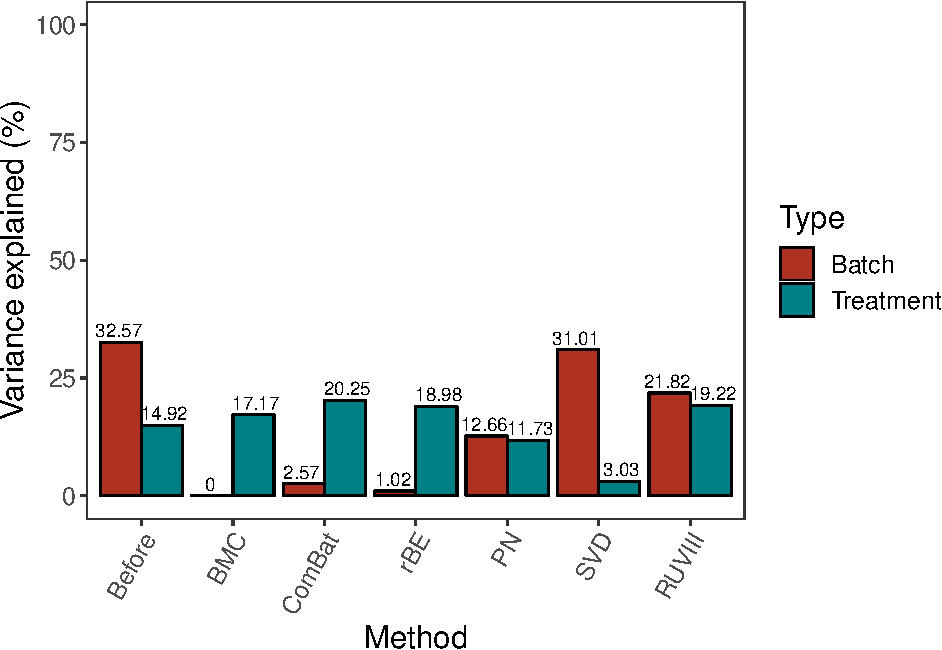
\includegraphics{Managing_batch_effects_files/figure-latex/unnamed-chunk-58-1.pdf}

\begin{Shaded}
\begin{Highlighting}[]
\KeywordTok{grid.arrange}\NormalTok{(ad.dens.before, ad.dens.percentile, }
\NormalTok{             ad.dens.svd, ad.dens.ruv, }\DataTypeTok{ncol =} \DecValTok{2}\NormalTok{)}
\end{Highlighting}
\end{Shaded}

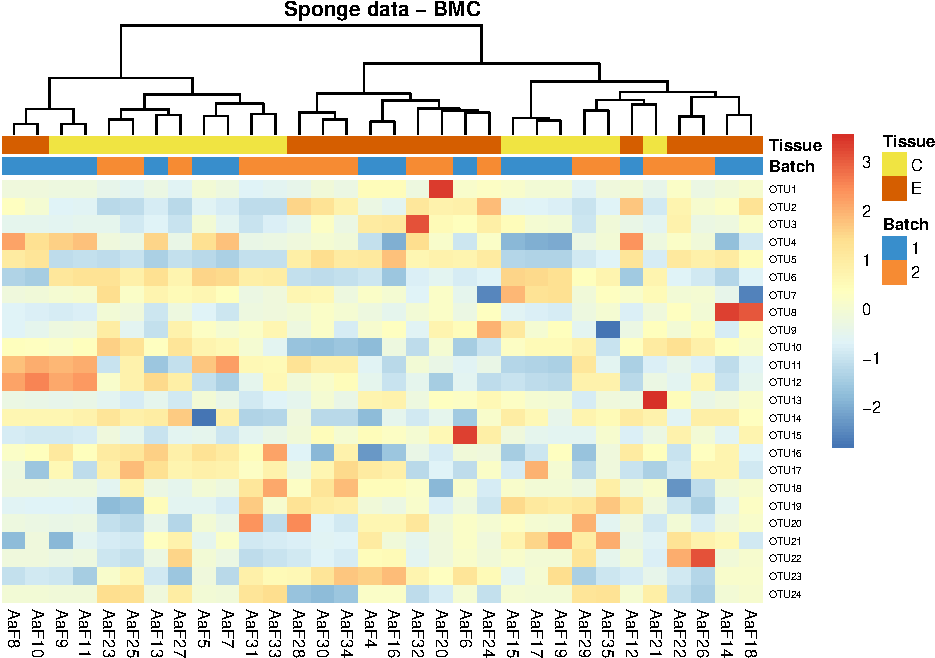
\includegraphics{Managing_batch_effects_files/figure-latex/unnamed-chunk-58-2.pdf}

Similar as sponge data, we can also assess the batch effect in AD data
using linear model.

\begin{Shaded}
\begin{Highlighting}[]
\CommentTok{#p-values}
\NormalTok{ad.lm.before <-}\StringTok{ }\KeywordTok{lm}\NormalTok{(ad.clr[ ,}\DecValTok{1}\NormalTok{] }\OperatorTok{~}\StringTok{ }\NormalTok{ad.trt }\OperatorTok{+}\StringTok{ }\NormalTok{ad.batch)}
\KeywordTok{anova}\NormalTok{(ad.lm.before)}
\end{Highlighting}
\end{Shaded}

\begin{verbatim}
## Analysis of Variance Table
## 
## Response: ad.clr[, 1]
##           Df Sum Sq Mean Sq F value    Pr(>F)    
## ad.trt     1  1.460  1.4605  3.1001   0.08272 .  
## ad.batch   4 32.889  8.2222 17.4532 6.168e-10 ***
## Residuals 69 32.506  0.4711                      
## ---
## Signif. codes:  0 '***' 0.001 '**' 0.01 '*' 0.05 '.' 0.1 ' ' 1
\end{verbatim}

\begin{Shaded}
\begin{Highlighting}[]
\CommentTok{#summary(ad.lm.before)}
\end{Highlighting}
\end{Shaded}

Before correction, the batch effect is statistically significant (P
\(<\) 0.001), as indicated in the \textbf{ad.batch} row.

\begin{Shaded}
\begin{Highlighting}[]
\NormalTok{ad.lm.bmc <-}\StringTok{ }\KeywordTok{lm}\NormalTok{(ad.bmc[ ,}\DecValTok{1}\NormalTok{] }\OperatorTok{~}\StringTok{ }\NormalTok{ad.trt }\OperatorTok{+}\StringTok{ }\NormalTok{ad.batch)}
\KeywordTok{anova}\NormalTok{(ad.lm.bmc)}
\end{Highlighting}
\end{Shaded}

\begin{verbatim}
## Analysis of Variance Table
## 
## Response: ad.bmc[, 1]
##           Df Sum Sq Mean Sq F value Pr(>F)
## ad.trt     1  0.631 0.63084  1.3391 0.2512
## ad.batch   4  0.036 0.00893  0.0190 0.9993
## Residuals 69 32.506 0.47110
\end{verbatim}

\begin{Shaded}
\begin{Highlighting}[]
\CommentTok{#summary(ad.lm.bmc)}
\end{Highlighting}
\end{Shaded}

After BMC correction, the batch effect is not statistically significant
(P \(>\) 0.05), as indicated in the \textbf{ad.batch} row.The results
from other batch correction methods are similar as BMC correction.

\begin{Shaded}
\begin{Highlighting}[]
\NormalTok{ad.lm.combat <-}\StringTok{ }\KeywordTok{lm}\NormalTok{(ad.combat[ ,}\DecValTok{1}\NormalTok{] }\OperatorTok{~}\StringTok{ }\NormalTok{ad.trt }\OperatorTok{+}\StringTok{ }\NormalTok{ad.batch)}
\KeywordTok{anova}\NormalTok{(ad.lm.combat)}
\CommentTok{#summary(ad.lm.combat)}

\NormalTok{ad.lm.limma <-}\StringTok{ }\KeywordTok{lm}\NormalTok{(ad.limma[ ,}\DecValTok{1}\NormalTok{] }\OperatorTok{~}\StringTok{ }\NormalTok{ad.trt }\OperatorTok{+}\StringTok{ }\NormalTok{ad.batch)}
\KeywordTok{anova}\NormalTok{(ad.lm.limma)}
\CommentTok{#summary(ad.lm.limma)}

\NormalTok{ad.lm.percentile <-}\StringTok{ }\KeywordTok{lm}\NormalTok{(ad.percentile[ ,}\DecValTok{1}\NormalTok{] }\OperatorTok{~}\StringTok{ }\NormalTok{ad.trt }\OperatorTok{+}\StringTok{ }\NormalTok{ad.batch)}
\KeywordTok{anova}\NormalTok{(ad.lm.percentile)}
\CommentTok{#summary(ad.lm.percentile)}

\NormalTok{ad.lm.svd <-}\StringTok{ }\KeywordTok{lm}\NormalTok{(ad.svd[ ,}\DecValTok{1}\NormalTok{] }\OperatorTok{~}\StringTok{ }\NormalTok{ad.trt }\OperatorTok{+}\StringTok{ }\NormalTok{ad.batch)}
\KeywordTok{anova}\NormalTok{(ad.lm.svd)}
\CommentTok{#summary(ad.lm.svd)}


\NormalTok{ad.lm.ruv <-}\StringTok{ }\KeywordTok{lm}\NormalTok{(ad.ruvIII[ ,}\DecValTok{1}\NormalTok{] }\OperatorTok{~}\StringTok{ }\NormalTok{ad.trt }\OperatorTok{+}\StringTok{ }\NormalTok{ad.batch)}
\KeywordTok{anova}\NormalTok{(ad.lm.ruv)}
\CommentTok{#summary(ad.lm.ruv)}
\end{Highlighting}
\end{Shaded}

The results of density plots and P-values of batch effects from linear
models reach a consesus with boxplots, the difference between two
batches are removed by BMC, ComBat, removeBatchEffect and RUVIII
correction.

\subsection{RLE plots}\label{rle-plots-1}

In sponge data, we group the samples according to the tissue (choanosome
/ ectosome) and generate two RLE plots respectively in all datasets
before and after batch correction with different methods:

\begin{Shaded}
\begin{Highlighting}[]
\CommentTok{# sponge data}
\CommentTok{# BMC}
\NormalTok{sponge.bmc_c <-}\StringTok{ }\NormalTok{sponge.bmc[sponge.trt }\OperatorTok{==}\StringTok{ 'C'}\NormalTok{, ]}
\NormalTok{sponge.bmc_e <-}\StringTok{ }\NormalTok{sponge.bmc[sponge.trt }\OperatorTok{==}\StringTok{ 'E'}\NormalTok{, ] }

\CommentTok{# ComBat}
\NormalTok{sponge.combat_c <-}\StringTok{ }\NormalTok{sponge.combat[sponge.trt }\OperatorTok{==}\StringTok{ 'C'}\NormalTok{, ]}
\NormalTok{sponge.combat_e <-}\StringTok{ }\NormalTok{sponge.combat[sponge.trt }\OperatorTok{==}\StringTok{ 'E'}\NormalTok{, ] }

\CommentTok{# rBE}
\NormalTok{sponge.limma_c <-}\StringTok{ }\NormalTok{sponge.limma[sponge.trt }\OperatorTok{==}\StringTok{ 'C'}\NormalTok{, ]}
\NormalTok{sponge.limma_e <-}\StringTok{ }\NormalTok{sponge.limma[sponge.trt }\OperatorTok{==}\StringTok{ 'E'}\NormalTok{, ] }

\CommentTok{# PN}
\NormalTok{sponge.percentile_c <-}\StringTok{ }\NormalTok{sponge.percentile[sponge.trt }\OperatorTok{==}\StringTok{ 'C'}\NormalTok{, ]}
\NormalTok{sponge.percentile_e <-}\StringTok{ }\NormalTok{sponge.percentile[sponge.trt }\OperatorTok{==}\StringTok{ 'E'}\NormalTok{, ] }

\CommentTok{# SVD}
\NormalTok{sponge.svd_c <-}\StringTok{ }\NormalTok{sponge.svd[sponge.trt }\OperatorTok{==}\StringTok{ 'C'}\NormalTok{, ]}
\NormalTok{sponge.svd_e <-}\StringTok{ }\NormalTok{sponge.svd[sponge.trt }\OperatorTok{==}\StringTok{ 'E'}\NormalTok{, ] }
\end{Highlighting}
\end{Shaded}

\begin{Shaded}
\begin{Highlighting}[]
\KeywordTok{par}\NormalTok{(}\DataTypeTok{mfrow =} \KeywordTok{c}\NormalTok{(}\DecValTok{2}\NormalTok{,}\DecValTok{3}\NormalTok{), }\DataTypeTok{mai =} \KeywordTok{c}\NormalTok{(}\FloatTok{0.4}\NormalTok{,}\FloatTok{0.6}\NormalTok{,}\FloatTok{0.3}\NormalTok{,}\FloatTok{0.1}\NormalTok{))}

\KeywordTok{RleMicroRna2}\NormalTok{(}\DataTypeTok{object =} \KeywordTok{t}\NormalTok{(sponge.before_c), }\DataTypeTok{batch =}\NormalTok{ sponge.batch_c, }
             \DataTypeTok{maintitle =} \StringTok{'Sponge: before (choanosome)'}\NormalTok{, }\DataTypeTok{title.cex =} \DecValTok{1}\NormalTok{)}

\KeywordTok{RleMicroRna2}\NormalTok{(}\DataTypeTok{object =} \KeywordTok{t}\NormalTok{(sponge.bmc_c), }\DataTypeTok{batch =}\NormalTok{ sponge.batch_c, }
             \DataTypeTok{maintitle =} \StringTok{'Sponge: BMC (choanosome)'}\NormalTok{, }\DataTypeTok{title.cex =} \DecValTok{1}\NormalTok{)}

\KeywordTok{RleMicroRna2}\NormalTok{(}\DataTypeTok{object =} \KeywordTok{t}\NormalTok{(sponge.combat_c), }\DataTypeTok{batch =}\NormalTok{ sponge.batch_c, }
             \DataTypeTok{maintitle =} \StringTok{'Sponge: ComBat (choanosome)'}\NormalTok{, }\DataTypeTok{title.cex =} \DecValTok{1}\NormalTok{)}

\KeywordTok{RleMicroRna2}\NormalTok{(}\DataTypeTok{object =} \KeywordTok{t}\NormalTok{(sponge.limma_c), }\DataTypeTok{batch =}\NormalTok{ sponge.batch_c, }
             \DataTypeTok{maintitle =} \StringTok{'Sponge: rBE (choanosome)'}\NormalTok{, }\DataTypeTok{title.cex =} \DecValTok{1}\NormalTok{)}

\KeywordTok{RleMicroRna2}\NormalTok{(}\DataTypeTok{object =} \KeywordTok{t}\NormalTok{(sponge.percentile_c), }\DataTypeTok{batch =}\NormalTok{ sponge.batch_c, }
             \DataTypeTok{maintitle =} \StringTok{'Sponge: PN (choanosome)'}\NormalTok{, }\DataTypeTok{title.cex =} \DecValTok{1}\NormalTok{)}

\KeywordTok{RleMicroRna2}\NormalTok{(}\DataTypeTok{object =} \KeywordTok{t}\NormalTok{(sponge.svd_c), }\DataTypeTok{batch =}\NormalTok{ sponge.batch_c, }
             \DataTypeTok{maintitle =} \StringTok{'Sponge: SVD (choanosome)'}\NormalTok{, }\DataTypeTok{title.cex =} \DecValTok{1}\NormalTok{)}
\end{Highlighting}
\end{Shaded}

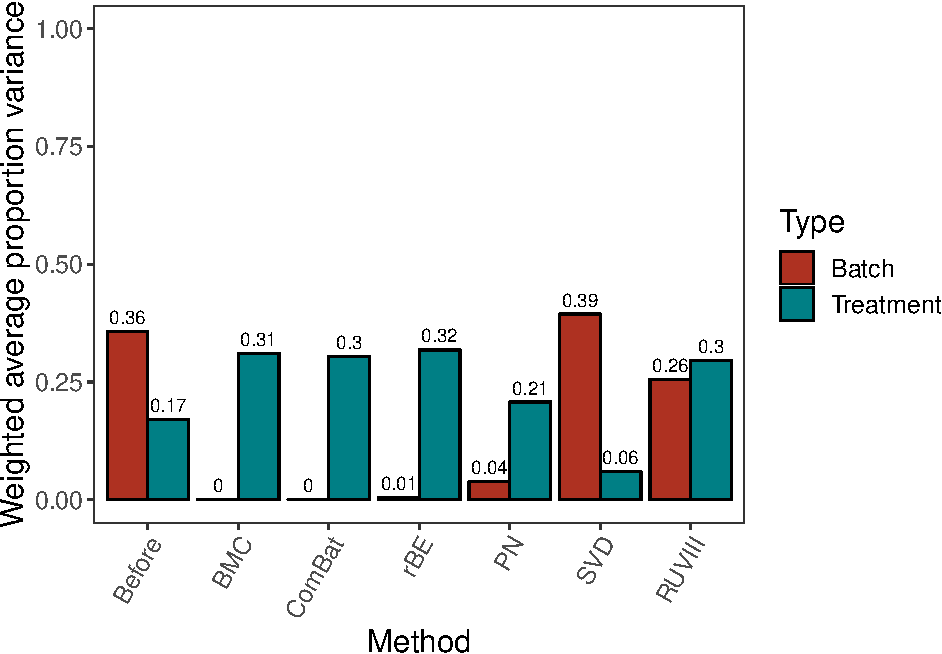
\includegraphics{Managing_batch_effects_files/figure-latex/unnamed-chunk-63-1.pdf}

\begin{Shaded}
\begin{Highlighting}[]
\KeywordTok{par}\NormalTok{(}\DataTypeTok{mfrow =} \KeywordTok{c}\NormalTok{(}\DecValTok{1}\NormalTok{,}\DecValTok{1}\NormalTok{))}
\end{Highlighting}
\end{Shaded}

In tissue choanosome of sponge data, the batch effect before correction
is not obvious as all medians of samples are close to zero, but Gel2 has
a greater interquartile range (IQR) than the other samples. Percentile
normalisation increased batch effects, as the samples after correction
are deviated from zero and the IQR is increased. Among other methods,
the IQR of all the box plots (samples) from different batches is
consistent after ComBat correction.

\begin{Shaded}
\begin{Highlighting}[]
\KeywordTok{par}\NormalTok{(}\DataTypeTok{mfrow =} \KeywordTok{c}\NormalTok{(}\DecValTok{2}\NormalTok{,}\DecValTok{3}\NormalTok{), }\DataTypeTok{mai =} \KeywordTok{c}\NormalTok{(}\FloatTok{0.4}\NormalTok{,}\FloatTok{0.6}\NormalTok{,}\FloatTok{0.3}\NormalTok{,}\FloatTok{0.1}\NormalTok{))}

\KeywordTok{RleMicroRna2}\NormalTok{(}\DataTypeTok{object =} \KeywordTok{t}\NormalTok{(sponge.before_e), }\DataTypeTok{batch =}\NormalTok{ sponge.batch_e, }
             \DataTypeTok{maintitle =} \StringTok{'Sponge: before (ectosome)'}\NormalTok{, }\DataTypeTok{title.cex =} \DecValTok{1}\NormalTok{)}

\KeywordTok{RleMicroRna2}\NormalTok{(}\DataTypeTok{object =} \KeywordTok{t}\NormalTok{(sponge.bmc_e), }\DataTypeTok{batch =}\NormalTok{ sponge.batch_e, }
             \DataTypeTok{maintitle =} \StringTok{'Sponge: BMC (ectosome)'}\NormalTok{, }\DataTypeTok{title.cex =} \DecValTok{1}\NormalTok{)}

\KeywordTok{RleMicroRna2}\NormalTok{(}\DataTypeTok{object =} \KeywordTok{t}\NormalTok{(sponge.combat_e), }\DataTypeTok{batch =}\NormalTok{ sponge.batch_e, }
             \DataTypeTok{maintitle =} \StringTok{'Sponge: ComBat (ectosome)'}\NormalTok{, }\DataTypeTok{title.cex =} \DecValTok{1}\NormalTok{)}

\KeywordTok{RleMicroRna2}\NormalTok{(}\DataTypeTok{object =} \KeywordTok{t}\NormalTok{(sponge.limma_e), }\DataTypeTok{batch =}\NormalTok{ sponge.batch_e, }
             \DataTypeTok{maintitle =} \StringTok{'Sponge: rBE (ectosome)'}\NormalTok{, }\DataTypeTok{title.cex =} \DecValTok{1}\NormalTok{)}

\KeywordTok{RleMicroRna2}\NormalTok{(}\DataTypeTok{object =} \KeywordTok{t}\NormalTok{(sponge.percentile_e), }\DataTypeTok{batch =}\NormalTok{ sponge.batch_e, }
             \DataTypeTok{maintitle =} \StringTok{'Sponge: PN (ectosome)'}\NormalTok{, }\DataTypeTok{title.cex =} \DecValTok{1}\NormalTok{)}

\KeywordTok{RleMicroRna2}\NormalTok{(}\DataTypeTok{object =} \KeywordTok{t}\NormalTok{(sponge.svd_e), }\DataTypeTok{batch =}\NormalTok{ sponge.batch_e, }
             \DataTypeTok{maintitle =} \StringTok{'Sponge: SVD (ectosome)'}\NormalTok{, }\DataTypeTok{title.cex =} \DecValTok{1}\NormalTok{)}
\end{Highlighting}
\end{Shaded}

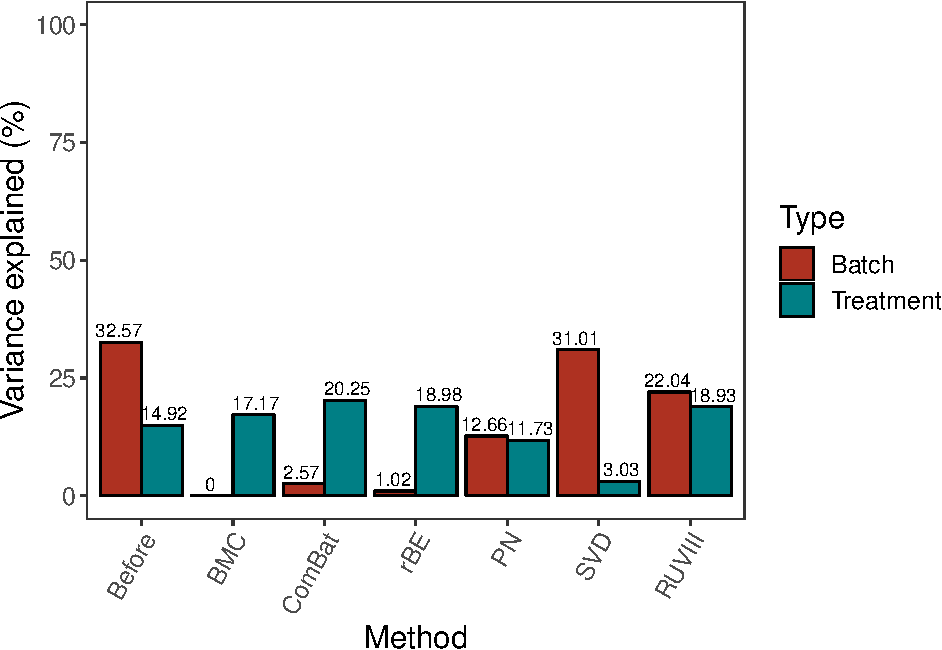
\includegraphics{Managing_batch_effects_files/figure-latex/unnamed-chunk-64-1.pdf}

\begin{Shaded}
\begin{Highlighting}[]
\KeywordTok{par}\NormalTok{(}\DataTypeTok{mfrow =} \KeywordTok{c}\NormalTok{(}\DecValTok{1}\NormalTok{,}\DecValTok{1}\NormalTok{))}
\end{Highlighting}
\end{Shaded}

In tissue ectosome of sponge data, batch effect is not easily detected,
but percentile normalisation increased batch variation.

In AD data, we group the samples according to the inital phenol
concentration (0-0.5 g/L / 1-2 g/L) and generate two RLE plots
respectively in all datasets before and after batch correction, as
sponge data:

\begin{Shaded}
\begin{Highlighting}[]
\CommentTok{# ad data}
\CommentTok{# BMC}
\NormalTok{ad.bmc_}\DecValTok{05}\NormalTok{ <-}\StringTok{ }\NormalTok{ad.bmc[ad.trt }\OperatorTok{==}\StringTok{ '0-0.5'}\NormalTok{, ]}
\NormalTok{ad.bmc_}\DecValTok{2}\NormalTok{ <-}\StringTok{ }\NormalTok{ad.bmc[ad.trt }\OperatorTok{==}\StringTok{ '1-2'}\NormalTok{, ]}

\CommentTok{# ComBat}
\NormalTok{ad.combat_}\DecValTok{05}\NormalTok{ <-}\StringTok{ }\NormalTok{ad.combat[ad.trt }\OperatorTok{==}\StringTok{ '0-0.5'}\NormalTok{, ]}
\NormalTok{ad.combat_}\DecValTok{2}\NormalTok{ <-}\StringTok{ }\NormalTok{ad.combat[ad.trt }\OperatorTok{==}\StringTok{ '1-2'}\NormalTok{, ]}

\CommentTok{# rBE}
\NormalTok{ad.limma_}\DecValTok{05}\NormalTok{ <-}\StringTok{ }\NormalTok{ad.limma[ad.trt }\OperatorTok{==}\StringTok{ '0-0.5'}\NormalTok{, ]}
\NormalTok{ad.limma_}\DecValTok{2}\NormalTok{ <-}\StringTok{ }\NormalTok{ad.limma[ad.trt }\OperatorTok{==}\StringTok{ '1-2'}\NormalTok{, ]}

\CommentTok{# PN}
\NormalTok{ad.percentile_}\DecValTok{05}\NormalTok{ <-}\StringTok{ }\NormalTok{ad.percentile[ad.trt }\OperatorTok{==}\StringTok{ '0-0.5'}\NormalTok{, ]}
\NormalTok{ad.percentile_}\DecValTok{2}\NormalTok{ <-}\StringTok{ }\NormalTok{ad.percentile[ad.trt }\OperatorTok{==}\StringTok{ '1-2'}\NormalTok{, ]}

\CommentTok{# SVD}
\NormalTok{ad.svd_}\DecValTok{05}\NormalTok{ <-}\StringTok{ }\NormalTok{ad.svd[ad.trt }\OperatorTok{==}\StringTok{ '0-0.5'}\NormalTok{, ]}
\NormalTok{ad.svd_}\DecValTok{2}\NormalTok{ <-}\StringTok{ }\NormalTok{ad.svd[ad.trt }\OperatorTok{==}\StringTok{ '1-2'}\NormalTok{, ]}

\CommentTok{# RUVIII}
\NormalTok{ad.ruv_}\DecValTok{05}\NormalTok{ <-}\StringTok{ }\NormalTok{ad.ruvIII[ad.trt }\OperatorTok{==}\StringTok{ '0-0.5'}\NormalTok{, ]}
\NormalTok{ad.ruv_}\DecValTok{2}\NormalTok{ <-}\StringTok{ }\NormalTok{ad.ruvIII[ad.trt }\OperatorTok{==}\StringTok{ '1-2'}\NormalTok{, ]}
\end{Highlighting}
\end{Shaded}

\begin{Shaded}
\begin{Highlighting}[]
\KeywordTok{par}\NormalTok{(}\DataTypeTok{mfrow =} \KeywordTok{c}\NormalTok{(}\DecValTok{2}\NormalTok{,}\DecValTok{2}\NormalTok{), }\DataTypeTok{mai =} \KeywordTok{c}\NormalTok{(}\FloatTok{0.5}\NormalTok{,}\FloatTok{0.8}\NormalTok{,}\FloatTok{0.3}\NormalTok{,}\FloatTok{0.1}\NormalTok{))}

\KeywordTok{RleMicroRna2}\NormalTok{(}\DataTypeTok{object =} \KeywordTok{t}\NormalTok{(ad.before_}\DecValTok{05}\NormalTok{), }\DataTypeTok{batch =}\NormalTok{ ad.batch_}\DecValTok{05}\NormalTok{, }
             \DataTypeTok{maintitle =} \StringTok{'AD: before (0-0.5 g/L)'}\NormalTok{, }\DataTypeTok{legend.cex =} \FloatTok{0.4}\NormalTok{, }
             \DataTypeTok{cex.xaxis =} \FloatTok{0.5}\NormalTok{)}

\KeywordTok{RleMicroRna2}\NormalTok{(}\DataTypeTok{object =} \KeywordTok{t}\NormalTok{(ad.bmc_}\DecValTok{05}\NormalTok{), }\DataTypeTok{batch =}\NormalTok{ ad.batch_}\DecValTok{05}\NormalTok{, }
             \DataTypeTok{maintitle =} \StringTok{'AD: BMC (0-0.5 g/L)'}\NormalTok{, }\DataTypeTok{legend.cex =} \FloatTok{0.4}\NormalTok{, }
             \DataTypeTok{cex.xaxis =} \FloatTok{0.5}\NormalTok{)}

\KeywordTok{RleMicroRna2}\NormalTok{(}\DataTypeTok{object =} \KeywordTok{t}\NormalTok{(ad.combat_}\DecValTok{05}\NormalTok{), }\DataTypeTok{batch =}\NormalTok{ ad.batch_}\DecValTok{05}\NormalTok{, }
             \DataTypeTok{maintitle =} \StringTok{'AD: ComBat (0-0.5 g/L)'}\NormalTok{, }\DataTypeTok{legend.cex =} \FloatTok{0.4}\NormalTok{, }
             \DataTypeTok{cex.xaxis =} \FloatTok{0.5}\NormalTok{)}

\KeywordTok{RleMicroRna2}\NormalTok{(}\DataTypeTok{object =} \KeywordTok{t}\NormalTok{(ad.limma_}\DecValTok{05}\NormalTok{), }\DataTypeTok{batch =}\NormalTok{ ad.batch_}\DecValTok{05}\NormalTok{, }
             \DataTypeTok{maintitle =} \StringTok{'AD: rBE (0-0.5 g/L)'}\NormalTok{, }\DataTypeTok{legend.cex =} \FloatTok{0.4}\NormalTok{, }
             \DataTypeTok{cex.xaxis =} \FloatTok{0.5}\NormalTok{)}
\end{Highlighting}
\end{Shaded}

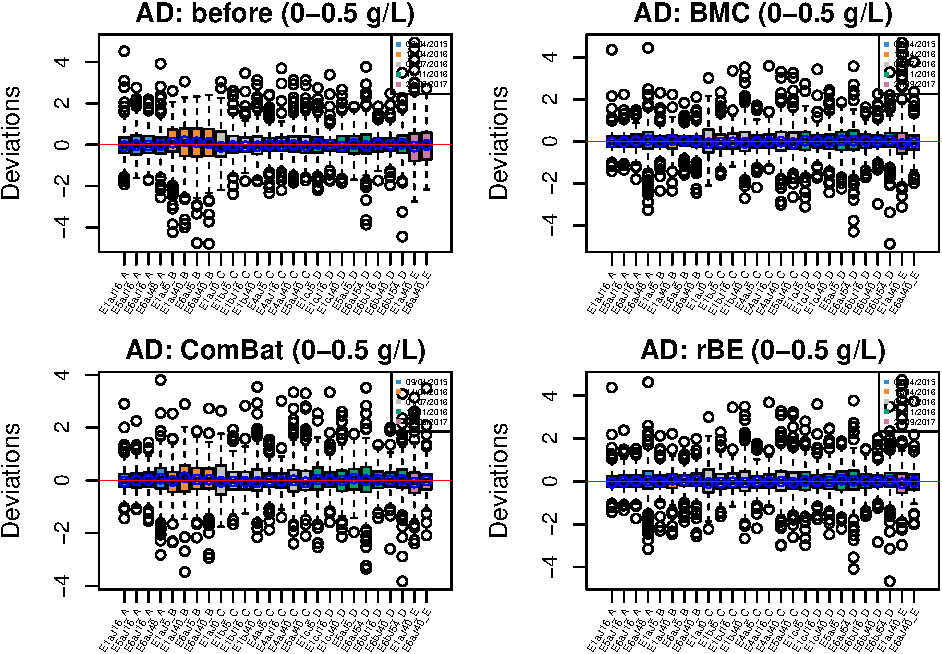
\includegraphics{Managing_batch_effects_files/figure-latex/unnamed-chunk-66-1.pdf}

\begin{Shaded}
\begin{Highlighting}[]
\KeywordTok{RleMicroRna2}\NormalTok{(}\DataTypeTok{object =} \KeywordTok{t}\NormalTok{(ad.percentile_}\DecValTok{05}\NormalTok{), }\DataTypeTok{batch =}\NormalTok{ ad.batch_}\DecValTok{05}\NormalTok{, }
             \DataTypeTok{maintitle =} \StringTok{'AD: PN (0-0.5 g/L)'}\NormalTok{, }\DataTypeTok{legend.cex =} \FloatTok{0.4}\NormalTok{, }
             \DataTypeTok{cex.xaxis =} \FloatTok{0.5}\NormalTok{)}

\KeywordTok{RleMicroRna2}\NormalTok{(}\DataTypeTok{object =} \KeywordTok{t}\NormalTok{(ad.svd_}\DecValTok{05}\NormalTok{), }\DataTypeTok{batch =}\NormalTok{ ad.batch_}\DecValTok{05}\NormalTok{, }
             \DataTypeTok{maintitle =} \StringTok{'AD: SVD (0-0.5 g/L)'}\NormalTok{, }\DataTypeTok{legend.cex =} \FloatTok{0.4}\NormalTok{, }
             \DataTypeTok{cex.xaxis =} \FloatTok{0.5}\NormalTok{)}

\KeywordTok{RleMicroRna2}\NormalTok{(}\DataTypeTok{object =} \KeywordTok{t}\NormalTok{(ad.ruv_}\DecValTok{05}\NormalTok{), }\DataTypeTok{batch =}\NormalTok{ ad.batch_}\DecValTok{05}\NormalTok{, }
             \DataTypeTok{maintitle =} \StringTok{'AD: RUVIII (0-0.5 g/L)'}\NormalTok{, }\DataTypeTok{legend.cex =} \FloatTok{0.4}\NormalTok{, }
             \DataTypeTok{cex.xaxis =} \FloatTok{0.5}\NormalTok{)}

\KeywordTok{par}\NormalTok{(}\DataTypeTok{mfrow =} \KeywordTok{c}\NormalTok{(}\DecValTok{1}\NormalTok{,}\DecValTok{1}\NormalTok{))}
\end{Highlighting}
\end{Shaded}

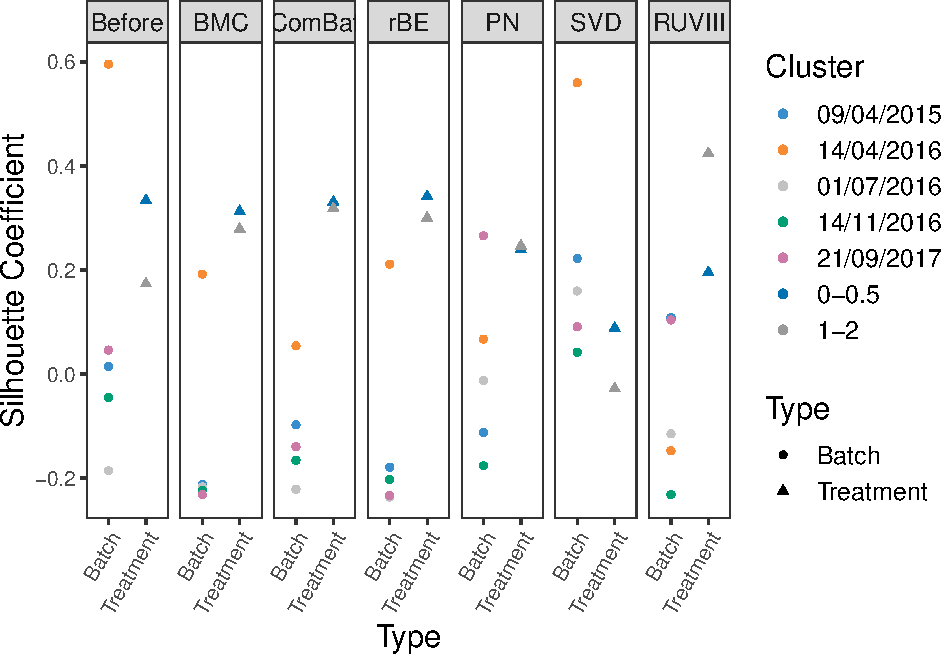
\includegraphics{Managing_batch_effects_files/figure-latex/unnamed-chunk-66-2.pdf}

In AD data with initial phenol concentration between 0-0.5 g/L, batch
effect is not easily detected, but percentile normalisation increased
batch variation.

\begin{Shaded}
\begin{Highlighting}[]
\KeywordTok{par}\NormalTok{(}\DataTypeTok{mfrow =} \KeywordTok{c}\NormalTok{(}\DecValTok{2}\NormalTok{,}\DecValTok{2}\NormalTok{), }\DataTypeTok{mai =} \KeywordTok{c}\NormalTok{(}\FloatTok{0.35}\NormalTok{,}\FloatTok{0.8}\NormalTok{,}\FloatTok{0.3}\NormalTok{,}\FloatTok{0.1}\NormalTok{))}

\KeywordTok{RleMicroRna2}\NormalTok{(}\DataTypeTok{object =} \KeywordTok{t}\NormalTok{(ad.before_}\DecValTok{2}\NormalTok{), }\DataTypeTok{batch =}\NormalTok{ ad.batch_}\DecValTok{2}\NormalTok{, }
             \DataTypeTok{maintitle =} \StringTok{'AD: before (1-2 g/L)'}\NormalTok{, }\DataTypeTok{legend.cex =} \FloatTok{0.4}\NormalTok{, }
             \DataTypeTok{cex.xaxis =} \FloatTok{0.3}\NormalTok{)}

\KeywordTok{RleMicroRna2}\NormalTok{(}\DataTypeTok{object =} \KeywordTok{t}\NormalTok{(ad.bmc_}\DecValTok{2}\NormalTok{), }\DataTypeTok{batch =}\NormalTok{ ad.batch_}\DecValTok{2}\NormalTok{, }
             \DataTypeTok{maintitle =} \StringTok{'AD: BMC (1-2 g/L)'}\NormalTok{, }\DataTypeTok{legend.cex =} \FloatTok{0.4}\NormalTok{, }
             \DataTypeTok{cex.xaxis =} \FloatTok{0.3}\NormalTok{)}

\KeywordTok{RleMicroRna2}\NormalTok{(}\DataTypeTok{object =} \KeywordTok{t}\NormalTok{(ad.combat_}\DecValTok{2}\NormalTok{), }\DataTypeTok{batch =}\NormalTok{ ad.batch_}\DecValTok{2}\NormalTok{, }
             \DataTypeTok{maintitle =} \StringTok{'AD: ComBat (1-2 g/L)'}\NormalTok{, }\DataTypeTok{legend.cex =} \FloatTok{0.4}\NormalTok{, }
             \DataTypeTok{cex.xaxis =} \FloatTok{0.3}\NormalTok{)}

\KeywordTok{RleMicroRna2}\NormalTok{(}\DataTypeTok{object =} \KeywordTok{t}\NormalTok{(ad.limma_}\DecValTok{2}\NormalTok{), }\DataTypeTok{batch =}\NormalTok{ ad.batch_}\DecValTok{2}\NormalTok{, }
             \DataTypeTok{maintitle =} \StringTok{'AD: rBE (1-2 g/L)'}\NormalTok{, }\DataTypeTok{legend.cex =} \FloatTok{0.4}\NormalTok{, }
             \DataTypeTok{cex.xaxis =} \FloatTok{0.3}\NormalTok{)}
\end{Highlighting}
\end{Shaded}

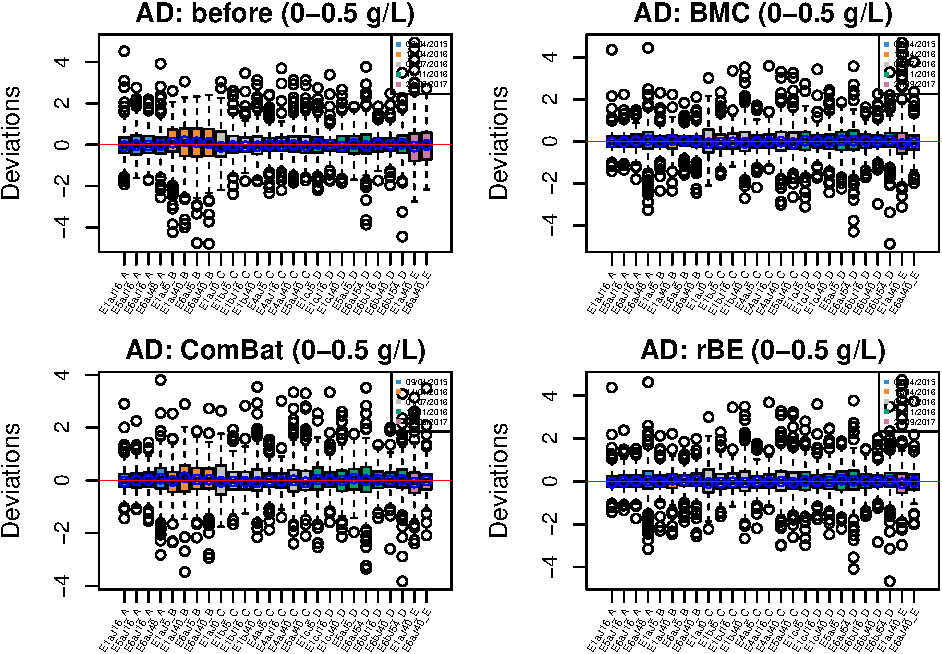
\includegraphics{Managing_batch_effects_files/figure-latex/unnamed-chunk-67-1.pdf}

\begin{Shaded}
\begin{Highlighting}[]
\KeywordTok{RleMicroRna2}\NormalTok{(}\DataTypeTok{object =} \KeywordTok{t}\NormalTok{(ad.percentile_}\DecValTok{2}\NormalTok{), }\DataTypeTok{batch =}\NormalTok{ ad.batch_}\DecValTok{2}\NormalTok{, }
             \DataTypeTok{maintitle =} \StringTok{'AD: PN (1-2 g/L)'}\NormalTok{, }\DataTypeTok{legend.cex =} \FloatTok{0.4}\NormalTok{, }
             \DataTypeTok{cex.xaxis =} \FloatTok{0.3}\NormalTok{)}

\KeywordTok{RleMicroRna2}\NormalTok{(}\DataTypeTok{object =} \KeywordTok{t}\NormalTok{(ad.svd_}\DecValTok{2}\NormalTok{), }\DataTypeTok{batch =}\NormalTok{ ad.batch_}\DecValTok{2}\NormalTok{, }
             \DataTypeTok{maintitle =} \StringTok{'AD: SVD (1-2 g/L)'}\NormalTok{, }\DataTypeTok{legend.cex =} \FloatTok{0.4}\NormalTok{, }
             \DataTypeTok{cex.xaxis =} \FloatTok{0.3}\NormalTok{)}

\KeywordTok{RleMicroRna2}\NormalTok{(}\DataTypeTok{object =} \KeywordTok{t}\NormalTok{(ad.ruv_}\DecValTok{2}\NormalTok{), }\DataTypeTok{batch =}\NormalTok{ ad.batch_}\DecValTok{2}\NormalTok{, }
             \DataTypeTok{maintitle =} \StringTok{'AD: RUVIII (1-2 g/L)'}\NormalTok{, }\DataTypeTok{legend.cex =} \FloatTok{0.4}\NormalTok{, }
             \DataTypeTok{cex.xaxis =} \FloatTok{0.3}\NormalTok{)}

\KeywordTok{par}\NormalTok{(}\DataTypeTok{mfrow =} \KeywordTok{c}\NormalTok{(}\DecValTok{1}\NormalTok{,}\DecValTok{1}\NormalTok{))}
\end{Highlighting}
\end{Shaded}

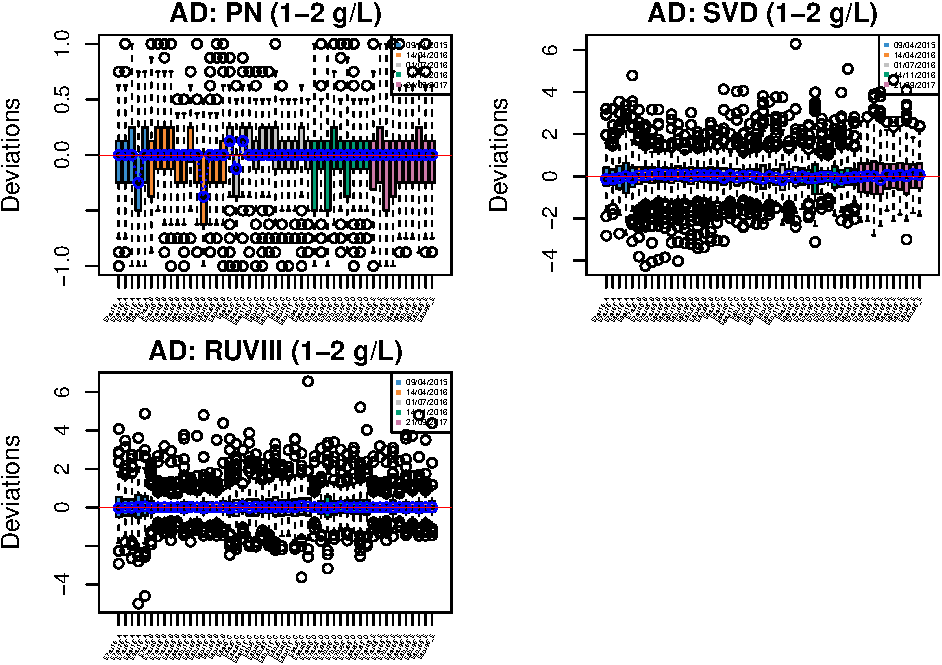
\includegraphics{Managing_batch_effects_files/figure-latex/unnamed-chunk-67-2.pdf}

In AD data with initial phenol concentration between 1-2 g/L, batch
effect is not easily detected, but percentile normalisation increased
batch variation.

\subsection{Heatmap}\label{heatmap-1}

We use the heatmap to visualise data clusters. Samples clustered by
batches instead of treatments indicate a batch effect.

\begin{Shaded}
\begin{Highlighting}[]
\CommentTok{# Sponge data}
\CommentTok{# before }
\NormalTok{sponge.tss.clr.scale <-}\StringTok{ }\KeywordTok{scale}\NormalTok{(sponge.tss.clr, }\DataTypeTok{center =}\NormalTok{ T, }\DataTypeTok{scale =}\NormalTok{ T) }
\CommentTok{# scale on OTUs}
\NormalTok{sponge.tss.clr.scale <-}\StringTok{ }\KeywordTok{scale}\NormalTok{(}\KeywordTok{t}\NormalTok{(sponge.tss.clr.scale), }\DataTypeTok{center =}\NormalTok{ T, }\DataTypeTok{scale =}\NormalTok{ T) }
\CommentTok{# scale on samples}

\NormalTok{sponge.anno_col <-}\StringTok{ }\KeywordTok{data.frame}\NormalTok{(}\DataTypeTok{Batch =}\NormalTok{ sponge.batch, }\DataTypeTok{Tissue =}\NormalTok{ sponge.trt)}
\NormalTok{sponge.anno_metabo_colors <-}\StringTok{ }\KeywordTok{list}\NormalTok{(}\DataTypeTok{Batch =} \KeywordTok{c}\NormalTok{(}\StringTok{'1'}\NormalTok{ =}\StringTok{ '#388ECC'}\NormalTok{, }\StringTok{'2'}\NormalTok{ =}\StringTok{ '#F68B33'}\NormalTok{), }
                                 \DataTypeTok{Tissue =} \KeywordTok{c}\NormalTok{(}\DataTypeTok{C =} \StringTok{'#F0E442'}\NormalTok{, }\DataTypeTok{E =} \StringTok{'#D55E00'}\NormalTok{))}


\KeywordTok{pheatmap}\NormalTok{(sponge.tss.clr.scale, }
         \DataTypeTok{scale =} \StringTok{'none'}\NormalTok{, }
         \DataTypeTok{cluster_rows =}\NormalTok{ F, }
         \DataTypeTok{cluster_cols =}\NormalTok{ T, }
         \DataTypeTok{fontsize_row =} \DecValTok{5}\NormalTok{, }\DataTypeTok{fontsize_col =} \DecValTok{8}\NormalTok{,}
         \DataTypeTok{fontsize =} \DecValTok{8}\NormalTok{,}
         \DataTypeTok{clustering_distance_rows =} \StringTok{'euclidean'}\NormalTok{,}
         \DataTypeTok{clustering_method =} \StringTok{'ward.D'}\NormalTok{,}
         \DataTypeTok{treeheight_row =} \DecValTok{30}\NormalTok{,}
         \DataTypeTok{annotation_col =}\NormalTok{ sponge.anno_col,}
         \DataTypeTok{annotation_colors =}\NormalTok{ sponge.anno_metabo_colors,}
         \DataTypeTok{border_color =} \StringTok{'NA'}\NormalTok{,}
         \DataTypeTok{main =} \StringTok{'Sponge data - before'}\NormalTok{)}
\end{Highlighting}
\end{Shaded}

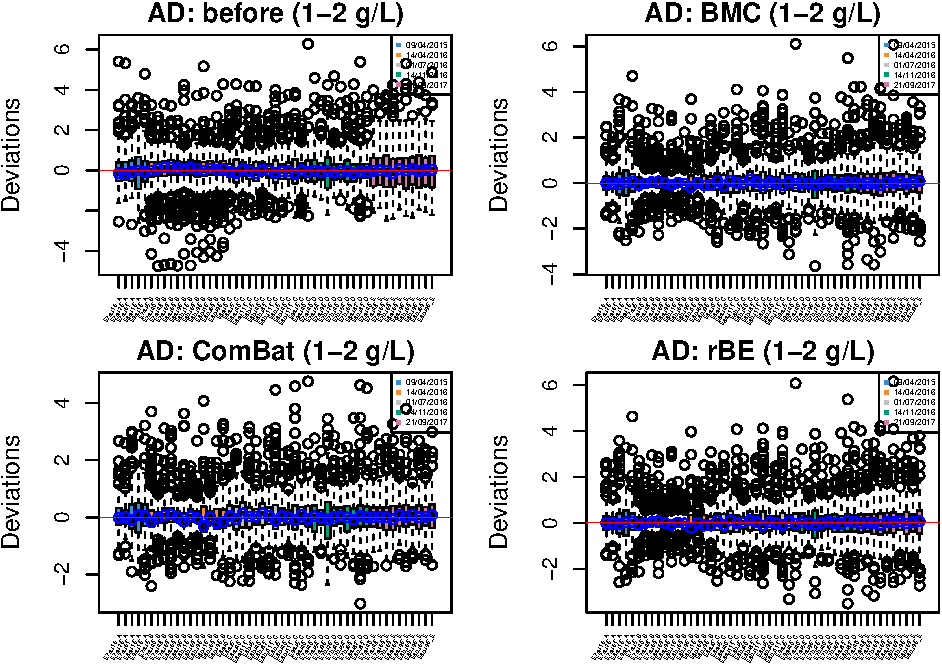
\includegraphics{Managing_batch_effects_files/figure-latex/unnamed-chunk-68-1.pdf}

Before correction, samples in sponge data are preferentially clustered
by batch instead of tissue type, indicating a batch effect.

\begin{Shaded}
\begin{Highlighting}[]
\CommentTok{# ComBat }
\NormalTok{sponge.combat.scale <-}\StringTok{ }\KeywordTok{scale}\NormalTok{(sponge.combat, }\DataTypeTok{center =}\NormalTok{ T, }\DataTypeTok{scale =}\NormalTok{ T) }
\CommentTok{# scale on OTUs}
\NormalTok{sponge.combat.scale <-}\StringTok{ }\KeywordTok{scale}\NormalTok{(}\KeywordTok{t}\NormalTok{(sponge.combat.scale), }\DataTypeTok{center =}\NormalTok{ T, }\DataTypeTok{scale =}\NormalTok{ T) }
\CommentTok{# scale on samples}

\KeywordTok{pheatmap}\NormalTok{(sponge.combat.scale, }
         \DataTypeTok{scale =} \StringTok{'none'}\NormalTok{, }
         \DataTypeTok{cluster_rows =}\NormalTok{ F, }
         \DataTypeTok{cluster_cols =}\NormalTok{ T, }
         \DataTypeTok{fontsize_row =} \DecValTok{5}\NormalTok{, }\DataTypeTok{fontsize_col =} \DecValTok{8}\NormalTok{,}
         \DataTypeTok{fontsize =} \DecValTok{8}\NormalTok{,}
         \DataTypeTok{clustering_distance_rows =} \StringTok{'euclidean'}\NormalTok{,}
         \DataTypeTok{clustering_method =} \StringTok{'ward.D'}\NormalTok{,}
         \DataTypeTok{treeheight_row =} \DecValTok{30}\NormalTok{,}
         \DataTypeTok{annotation_col =}\NormalTok{ sponge.anno_col,}
         \DataTypeTok{annotation_colors =}\NormalTok{ sponge.anno_metabo_colors,}
         \DataTypeTok{border_color =} \StringTok{'NA'}\NormalTok{,}
         \DataTypeTok{main =} \StringTok{'Sponge data - ComBat'}\NormalTok{)}
\end{Highlighting}
\end{Shaded}

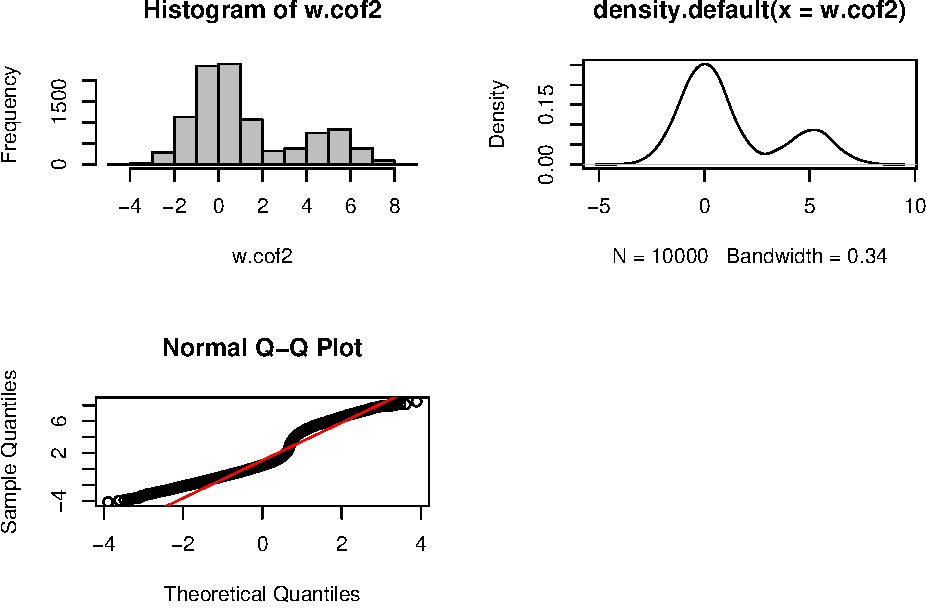
\includegraphics{Managing_batch_effects_files/figure-latex/unnamed-chunk-69-1.pdf}

After batch correction with ComBat, the data are clustered by tissues
rather than batches, therefore, ComBat not only removed batch effects,
but also disengaged the effect of interest. The results from batch
correction with other methods are similar.

\begin{Shaded}
\begin{Highlighting}[]
\CommentTok{# BMC }
\NormalTok{sponge.bmc.scale <-}\StringTok{ }\KeywordTok{scale}\NormalTok{(sponge.bmc, }\DataTypeTok{center =}\NormalTok{ T, }\DataTypeTok{scale =}\NormalTok{ T) }
\CommentTok{# scale on OTUs}
\NormalTok{sponge.bmc.scale <-}\StringTok{ }\KeywordTok{scale}\NormalTok{(}\KeywordTok{t}\NormalTok{(sponge.bmc.scale), }\DataTypeTok{center =}\NormalTok{ T, }\DataTypeTok{scale =}\NormalTok{ T) }
\CommentTok{# scale on samples}

\KeywordTok{pheatmap}\NormalTok{(sponge.bmc.scale, }
         \DataTypeTok{scale =} \StringTok{'none'}\NormalTok{, }
         \DataTypeTok{cluster_rows =}\NormalTok{ F, }
         \DataTypeTok{cluster_cols =}\NormalTok{ T, }
         \DataTypeTok{fontsize_row =} \DecValTok{5}\NormalTok{, }\DataTypeTok{fontsize_col =} \DecValTok{8}\NormalTok{,}
         \DataTypeTok{fontsize =} \DecValTok{8}\NormalTok{,}
         \DataTypeTok{clustering_distance_rows =} \StringTok{'euclidean'}\NormalTok{,}
         \DataTypeTok{clustering_method =} \StringTok{'ward.D'}\NormalTok{,}
         \DataTypeTok{treeheight_row =} \DecValTok{30}\NormalTok{,}
         \DataTypeTok{annotation_col =}\NormalTok{ sponge.anno_col,}
         \DataTypeTok{annotation_colors =}\NormalTok{ sponge.anno_metabo_colors,}
         \DataTypeTok{border_color =} \StringTok{'NA'}\NormalTok{,}
         \DataTypeTok{main =} \StringTok{'Sponge data - BMC'}\NormalTok{)}


\CommentTok{# removeBatchEffect}
\NormalTok{sponge.limma.scale <-}\StringTok{ }\KeywordTok{scale}\NormalTok{(sponge.limma, }\DataTypeTok{center =}\NormalTok{ T, }\DataTypeTok{scale =}\NormalTok{ T) }
\CommentTok{# scale on OTUs}
\NormalTok{sponge.limma.scale <-}\StringTok{ }\KeywordTok{scale}\NormalTok{(}\KeywordTok{t}\NormalTok{(sponge.limma.scale), }\DataTypeTok{center =}\NormalTok{ T, }\DataTypeTok{scale =}\NormalTok{ T) }
\CommentTok{# scale on samples}

\KeywordTok{pheatmap}\NormalTok{(sponge.limma.scale, }
         \DataTypeTok{scale =} \StringTok{'none'}\NormalTok{, }
         \DataTypeTok{cluster_rows =}\NormalTok{ F, }
         \DataTypeTok{cluster_cols =}\NormalTok{ T, }
         \DataTypeTok{fontsize_row =} \DecValTok{5}\NormalTok{, }\DataTypeTok{fontsize_col =} \DecValTok{8}\NormalTok{,}
         \DataTypeTok{fontsize =} \DecValTok{8}\NormalTok{,}
         \DataTypeTok{clustering_distance_rows =} \StringTok{'euclidean'}\NormalTok{,}
         \DataTypeTok{clustering_method =} \StringTok{'ward.D'}\NormalTok{,}
         \DataTypeTok{treeheight_row =} \DecValTok{30}\NormalTok{,}
         \DataTypeTok{annotation_col =}\NormalTok{ sponge.anno_col,}
         \DataTypeTok{annotation_colors =}\NormalTok{ sponge.anno_metabo_colors,}
         \DataTypeTok{border_color =} \StringTok{'NA'}\NormalTok{,}
         \DataTypeTok{main =} \StringTok{'Sponge data - removeBatchEffect'}\NormalTok{)}

\CommentTok{# percentile normalisation}
\NormalTok{sponge.percentile.scale <-}\StringTok{ }\KeywordTok{scale}\NormalTok{(sponge.percentile, }\DataTypeTok{center =}\NormalTok{ T, }\DataTypeTok{scale =}\NormalTok{ T) }
\CommentTok{# scale on OTUs}
\NormalTok{sponge.percentile.scale <-}\StringTok{ }\KeywordTok{scale}\NormalTok{(}\KeywordTok{t}\NormalTok{(sponge.percentile.scale), }\DataTypeTok{center =}\NormalTok{ T, }\DataTypeTok{scale =}\NormalTok{ T) }
\CommentTok{# scale on samples}

\KeywordTok{pheatmap}\NormalTok{(sponge.percentile.scale, }
         \DataTypeTok{scale =} \StringTok{'none'}\NormalTok{, }
         \DataTypeTok{cluster_rows =}\NormalTok{ F, }
         \DataTypeTok{cluster_cols =}\NormalTok{ T, }
         \DataTypeTok{fontsize_row =} \DecValTok{5}\NormalTok{, }\DataTypeTok{fontsize_col =} \DecValTok{8}\NormalTok{,}
         \DataTypeTok{fontsize =} \DecValTok{8}\NormalTok{,}
         \DataTypeTok{clustering_distance_rows =} \StringTok{'euclidean'}\NormalTok{,}
         \DataTypeTok{clustering_method =} \StringTok{'ward.D'}\NormalTok{,}
         \DataTypeTok{treeheight_row =} \DecValTok{30}\NormalTok{,}
         \DataTypeTok{annotation_col =}\NormalTok{ sponge.anno_col,}
         \DataTypeTok{annotation_colors =}\NormalTok{ sponge.anno_metabo_colors,}
         \DataTypeTok{border_color =} \StringTok{'NA'}\NormalTok{,}
         \DataTypeTok{main =} \StringTok{'Sponge data - percentile norm'}\NormalTok{)}


\CommentTok{# SVD}
\NormalTok{sponge.svd.scale <-}\StringTok{ }\KeywordTok{scale}\NormalTok{(sponge.svd, }\DataTypeTok{center =}\NormalTok{ T, }\DataTypeTok{scale =}\NormalTok{ T) }
\CommentTok{# scale on OTUs}
\NormalTok{sponge.svd.scale <-}\StringTok{ }\KeywordTok{scale}\NormalTok{(}\KeywordTok{t}\NormalTok{(sponge.svd.scale), }\DataTypeTok{center =}\NormalTok{ T, }\DataTypeTok{scale =}\NormalTok{ T) }
\CommentTok{# scale on samples}

\KeywordTok{pheatmap}\NormalTok{(sponge.svd.scale, }
         \DataTypeTok{scale =} \StringTok{'none'}\NormalTok{, }
         \DataTypeTok{cluster_rows =}\NormalTok{ F, }
         \DataTypeTok{cluster_cols =}\NormalTok{ T, }
         \DataTypeTok{fontsize_row =} \DecValTok{5}\NormalTok{, }\DataTypeTok{fontsize_col =} \DecValTok{8}\NormalTok{,}
         \DataTypeTok{fontsize =} \DecValTok{8}\NormalTok{,}
         \DataTypeTok{clustering_distance_rows =} \StringTok{'euclidean'}\NormalTok{,}
         \DataTypeTok{clustering_method =} \StringTok{'ward.D'}\NormalTok{,}
         \DataTypeTok{treeheight_row =} \DecValTok{30}\NormalTok{,}
         \DataTypeTok{annotation_col =}\NormalTok{ sponge.anno_col,}
         \DataTypeTok{annotation_colors =}\NormalTok{ sponge.anno_metabo_colors,}
         \DataTypeTok{border_color =} \StringTok{'NA'}\NormalTok{,}
         \DataTypeTok{main =} \StringTok{'Sponge data - SVD'}\NormalTok{)}
\end{Highlighting}
\end{Shaded}

In the heatmap of AD data before batch correction, samples within batch
14/04/2016 are clustered and distinct from other samples, indicating a
batch effect.

\begin{Shaded}
\begin{Highlighting}[]
\CommentTok{# AD data}
\CommentTok{# before }
\NormalTok{ad.clr.scale <-}\StringTok{ }\KeywordTok{scale}\NormalTok{(ad.clr, }\DataTypeTok{center =}\NormalTok{ T, }\DataTypeTok{scale =}\NormalTok{ T) }\CommentTok{# scale on OTUs}
\NormalTok{ad.clr.scale <-}\StringTok{ }\KeywordTok{scale}\NormalTok{(}\KeywordTok{t}\NormalTok{(ad.clr.scale), }\DataTypeTok{center =}\NormalTok{ T, }\DataTypeTok{scale =}\NormalTok{ T) }\CommentTok{# scale on samples}

\NormalTok{ad.anno_col <-}\StringTok{ }\KeywordTok{data.frame}\NormalTok{(}\DataTypeTok{Batch =}\NormalTok{ ad.batch, }\DataTypeTok{Treatment =}\NormalTok{ ad.trt)}
\NormalTok{ad.anno_metabo_colors <-}\StringTok{ }\KeywordTok{list}\NormalTok{(}\DataTypeTok{Batch =} \KeywordTok{c}\NormalTok{(}\StringTok{'09/04/2015'}\NormalTok{ =}\StringTok{ '#388ECC'}\NormalTok{, }
                                       \StringTok{'14/04/2016'}\NormalTok{ =}\StringTok{ '#F68B33'}\NormalTok{, }
                                       \StringTok{'01/07/2016'}\NormalTok{ =}\StringTok{ '#C2C2C2'}\NormalTok{, }
                                       \StringTok{'14/11/2016'}\NormalTok{ =}\StringTok{ '#009E73'}\NormalTok{, }
                                       \StringTok{'21/09/2017'}\NormalTok{ =}\StringTok{ '#CC79A7'}\NormalTok{), }
                             \DataTypeTok{Treatment =} \KeywordTok{c}\NormalTok{(}\StringTok{'0-0.5'}\NormalTok{ =}\StringTok{ '#0072B2'}\NormalTok{, }\StringTok{'1-2'}\NormalTok{ =}\StringTok{ '#999999'}\NormalTok{))}


\KeywordTok{pheatmap}\NormalTok{(ad.clr.scale, }
         \DataTypeTok{scale =} \StringTok{'none'}\NormalTok{, }
         \DataTypeTok{cluster_rows =}\NormalTok{ F, }
         \DataTypeTok{cluster_cols =}\NormalTok{ T, }
         \DataTypeTok{fontsize_row =} \DecValTok{4}\NormalTok{, }\DataTypeTok{fontsize_col =} \DecValTok{6}\NormalTok{,}
         \DataTypeTok{fontsize =} \DecValTok{8}\NormalTok{,}
         \DataTypeTok{clustering_distance_rows =} \StringTok{'euclidean'}\NormalTok{,}
         \DataTypeTok{clustering_method =} \StringTok{'ward.D'}\NormalTok{,}
         \DataTypeTok{treeheight_row =} \DecValTok{30}\NormalTok{,}
         \DataTypeTok{annotation_col =}\NormalTok{ ad.anno_col,}
         \DataTypeTok{annotation_colors =}\NormalTok{ ad.anno_metabo_colors,}
         \DataTypeTok{border_color =} \StringTok{'NA'}\NormalTok{,}
         \DataTypeTok{main =} \StringTok{'AD data - before'}\NormalTok{)}
\end{Highlighting}
\end{Shaded}

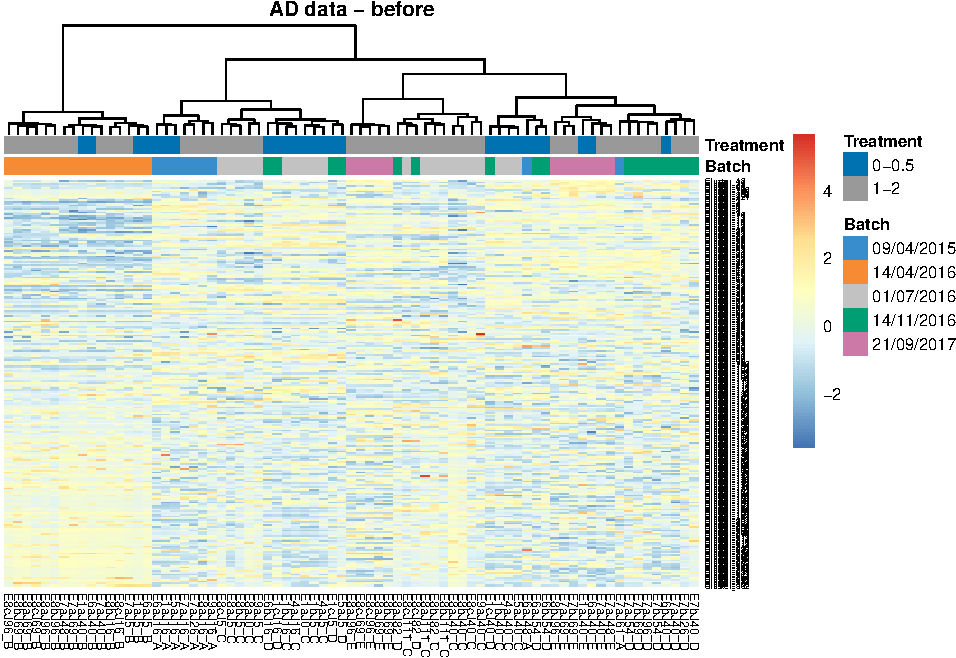
\includegraphics{Managing_batch_effects_files/figure-latex/unnamed-chunk-71-1.pdf}

\begin{Shaded}
\begin{Highlighting}[]
\CommentTok{# removeBatchEffect}
\NormalTok{ad.limma.scale <-}\StringTok{ }\KeywordTok{scale}\NormalTok{(ad.limma, }\DataTypeTok{center =}\NormalTok{ T, }\DataTypeTok{scale =}\NormalTok{ T) }\CommentTok{# scale on OTUs}
\NormalTok{ad.limma.scale <-}\StringTok{ }\KeywordTok{scale}\NormalTok{(}\KeywordTok{t}\NormalTok{(ad.limma.scale), }\DataTypeTok{center =}\NormalTok{ T, }\DataTypeTok{scale =}\NormalTok{ T) }\CommentTok{# scale on samples}

\KeywordTok{pheatmap}\NormalTok{(ad.limma.scale, }
         \DataTypeTok{scale =} \StringTok{'none'}\NormalTok{, }
         \DataTypeTok{cluster_rows =}\NormalTok{ F, }
         \DataTypeTok{cluster_cols =}\NormalTok{ T, }
         \DataTypeTok{fontsize_row =} \DecValTok{4}\NormalTok{, }\DataTypeTok{fontsize_col =} \DecValTok{6}\NormalTok{,}
         \DataTypeTok{fontsize =} \DecValTok{8}\NormalTok{,}
         \DataTypeTok{clustering_distance_rows =} \StringTok{'euclidean'}\NormalTok{,}
         \DataTypeTok{clustering_method =} \StringTok{'ward.D'}\NormalTok{,}
         \DataTypeTok{treeheight_row =} \DecValTok{30}\NormalTok{,}
         \DataTypeTok{annotation_col =}\NormalTok{ ad.anno_col,}
         \DataTypeTok{annotation_colors =}\NormalTok{ ad.anno_metabo_colors,}
         \DataTypeTok{border_color =} \StringTok{'NA'}\NormalTok{,}
         \DataTypeTok{main =} \StringTok{'AD data - removeBatchEffect'}\NormalTok{)}
\end{Highlighting}
\end{Shaded}

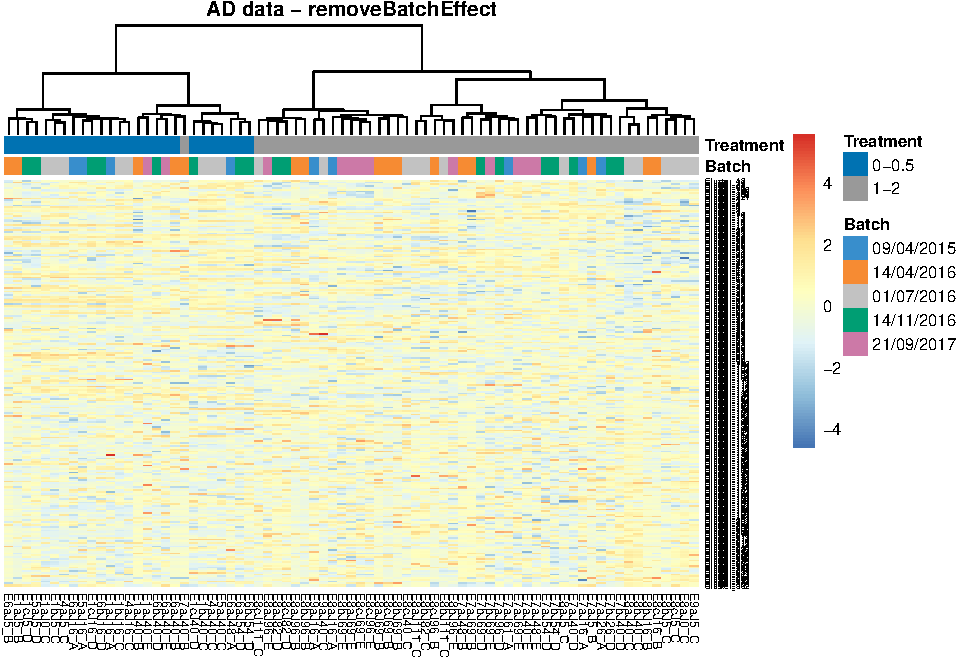
\includegraphics{Managing_batch_effects_files/figure-latex/unnamed-chunk-72-1.pdf}

After batch correction with removeBatchEffect, the data are almost
clustered by treatments rather than batches, therefore,
removeBatchEffect not only removed batch effects, but also disengaged
the treatment effects. The results from batch correction with other
methods are similar.

\begin{Shaded}
\begin{Highlighting}[]
\CommentTok{# BMC}
\NormalTok{ad.bmc.scale <-}\StringTok{ }\KeywordTok{scale}\NormalTok{(ad.bmc, }\DataTypeTok{center =}\NormalTok{ T, }\DataTypeTok{scale =}\NormalTok{ T) }\CommentTok{# scale on OTUs}
\NormalTok{ad.bmc.scale <-}\StringTok{ }\KeywordTok{scale}\NormalTok{(}\KeywordTok{t}\NormalTok{(ad.bmc.scale), }\DataTypeTok{center =}\NormalTok{ T, }\DataTypeTok{scale =}\NormalTok{ T) }\CommentTok{# scale on samples}

\KeywordTok{pheatmap}\NormalTok{(ad.bmc.scale, }
         \DataTypeTok{scale =} \StringTok{'none'}\NormalTok{, }
         \DataTypeTok{cluster_rows =}\NormalTok{ F, }
         \DataTypeTok{cluster_cols =}\NormalTok{ T, }
         \DataTypeTok{fontsize_row =} \DecValTok{4}\NormalTok{, }\DataTypeTok{fontsize_col =} \DecValTok{6}\NormalTok{,}
         \DataTypeTok{fontsize =} \DecValTok{8}\NormalTok{,}
         \DataTypeTok{clustering_distance_rows =} \StringTok{'euclidean'}\NormalTok{,}
         \DataTypeTok{clustering_method =} \StringTok{'ward.D'}\NormalTok{,}
         \DataTypeTok{treeheight_row =} \DecValTok{30}\NormalTok{,}
         \DataTypeTok{annotation_col =}\NormalTok{ ad.anno_col,}
         \DataTypeTok{annotation_colors =}\NormalTok{ ad.anno_metabo_colors,}
         \DataTypeTok{border_color =} \StringTok{'NA'}\NormalTok{,}
         \DataTypeTok{main =} \StringTok{'AD data - BMC'}\NormalTok{)}

\CommentTok{# ComBat}
\NormalTok{ad.combat.scale <-}\StringTok{ }\KeywordTok{scale}\NormalTok{(ad.combat, }\DataTypeTok{center =}\NormalTok{ T, }\DataTypeTok{scale =}\NormalTok{ T) }\CommentTok{# scale on OTUs}
\NormalTok{ad.combat.scale <-}\StringTok{ }\KeywordTok{scale}\NormalTok{(}\KeywordTok{t}\NormalTok{(ad.combat.scale), }\DataTypeTok{center =}\NormalTok{ T, }\DataTypeTok{scale =}\NormalTok{ T) }\CommentTok{# scale on samples}

\KeywordTok{pheatmap}\NormalTok{(ad.combat.scale, }
         \DataTypeTok{scale =} \StringTok{'none'}\NormalTok{, }
         \DataTypeTok{cluster_rows =}\NormalTok{ F, }
         \DataTypeTok{cluster_cols =}\NormalTok{ T, }
         \DataTypeTok{fontsize_row =} \DecValTok{4}\NormalTok{, }\DataTypeTok{fontsize_col =} \DecValTok{6}\NormalTok{,}
         \DataTypeTok{fontsize =} \DecValTok{8}\NormalTok{,}
         \DataTypeTok{clustering_distance_rows =} \StringTok{'euclidean'}\NormalTok{,}
         \DataTypeTok{clustering_method =} \StringTok{'ward.D'}\NormalTok{,}
         \DataTypeTok{treeheight_row =} \DecValTok{30}\NormalTok{,}
         \DataTypeTok{annotation_col =}\NormalTok{ ad.anno_col,}
         \DataTypeTok{annotation_colors =}\NormalTok{ ad.anno_metabo_colors,}
         \DataTypeTok{border_color =} \StringTok{'NA'}\NormalTok{,}
         \DataTypeTok{main =} \StringTok{'AD data - ComBat'}\NormalTok{)}



\CommentTok{# percentile normalisation}
\NormalTok{ad.percentile.scale <-}\StringTok{ }\KeywordTok{scale}\NormalTok{(ad.percentile, }\DataTypeTok{center =}\NormalTok{ T, }\DataTypeTok{scale =}\NormalTok{ T) }\CommentTok{# scale on OTUs}
\NormalTok{ad.percentile.scale <-}\StringTok{ }\KeywordTok{scale}\NormalTok{(}\KeywordTok{t}\NormalTok{(ad.percentile.scale), }\DataTypeTok{center =}\NormalTok{ T, }\DataTypeTok{scale =}\NormalTok{ T) }\CommentTok{# scale on samples}

\KeywordTok{pheatmap}\NormalTok{(ad.percentile.scale, }
         \DataTypeTok{scale =} \StringTok{'none'}\NormalTok{, }
         \DataTypeTok{cluster_rows =}\NormalTok{ F, }
         \DataTypeTok{cluster_cols =}\NormalTok{ T, }
         \DataTypeTok{fontsize_row =} \DecValTok{4}\NormalTok{, }\DataTypeTok{fontsize_col =} \DecValTok{6}\NormalTok{,}
         \DataTypeTok{fontsize =} \DecValTok{8}\NormalTok{,}
         \DataTypeTok{clustering_distance_rows =} \StringTok{'euclidean'}\NormalTok{,}
         \DataTypeTok{clustering_method =} \StringTok{'ward.D'}\NormalTok{,}
         \DataTypeTok{treeheight_row =} \DecValTok{30}\NormalTok{,}
         \DataTypeTok{annotation_col =}\NormalTok{ ad.anno_col,}
         \DataTypeTok{annotation_colors =}\NormalTok{ ad.anno_metabo_colors,}
         \DataTypeTok{border_color =} \StringTok{'NA'}\NormalTok{,}
         \DataTypeTok{main =} \StringTok{'AD data - percentile norm'}\NormalTok{)}

\CommentTok{# SVD}
\NormalTok{ad.svd.scale <-}\StringTok{ }\KeywordTok{scale}\NormalTok{(ad.svd, }\DataTypeTok{center =}\NormalTok{ T, }\DataTypeTok{scale =}\NormalTok{ T) }\CommentTok{# scale on OTUs}
\NormalTok{ad.svd.scale <-}\StringTok{ }\KeywordTok{scale}\NormalTok{(}\KeywordTok{t}\NormalTok{(ad.svd.scale), }\DataTypeTok{center =}\NormalTok{ T, }\DataTypeTok{scale =}\NormalTok{ T) }\CommentTok{# scale on samples}

\KeywordTok{pheatmap}\NormalTok{(ad.svd.scale, }
         \DataTypeTok{scale =} \StringTok{'none'}\NormalTok{, }
         \DataTypeTok{cluster_rows =}\NormalTok{ F, }
         \DataTypeTok{cluster_cols =}\NormalTok{ T, }
         \DataTypeTok{fontsize_row =} \DecValTok{4}\NormalTok{, }\DataTypeTok{fontsize_col =} \DecValTok{6}\NormalTok{,}
         \DataTypeTok{fontsize =} \DecValTok{8}\NormalTok{,}
         \DataTypeTok{clustering_distance_rows =} \StringTok{'euclidean'}\NormalTok{,}
         \DataTypeTok{clustering_method =} \StringTok{'ward.D'}\NormalTok{,}
         \DataTypeTok{treeheight_row =} \DecValTok{30}\NormalTok{,}
         \DataTypeTok{annotation_col =}\NormalTok{ ad.anno_col,}
         \DataTypeTok{annotation_colors =}\NormalTok{ ad.anno_metabo_colors,}
         \DataTypeTok{border_color =} \StringTok{'NA'}\NormalTok{,}
         \DataTypeTok{main =} \StringTok{'AD data - SVD'}\NormalTok{)}


\CommentTok{# RUVIII}
\NormalTok{ad.ruv.scale <-}\StringTok{ }\KeywordTok{scale}\NormalTok{(ad.ruvIII, }\DataTypeTok{center =}\NormalTok{ T, }\DataTypeTok{scale =}\NormalTok{ T) }\CommentTok{# scale on OTUs}
\NormalTok{ad.ruv.scale <-}\StringTok{ }\KeywordTok{scale}\NormalTok{(}\KeywordTok{t}\NormalTok{(ad.ruv.scale), }\DataTypeTok{center =}\NormalTok{ T, }\DataTypeTok{scale =}\NormalTok{ T) }\CommentTok{# scale on samples}

\KeywordTok{pheatmap}\NormalTok{(ad.ruv.scale, }
         \DataTypeTok{scale =} \StringTok{'none'}\NormalTok{, }
         \DataTypeTok{cluster_rows =}\NormalTok{ F, }
         \DataTypeTok{cluster_cols =}\NormalTok{ T, }
         \DataTypeTok{fontsize_row =} \DecValTok{4}\NormalTok{, }\DataTypeTok{fontsize_col =} \DecValTok{6}\NormalTok{,}
         \DataTypeTok{fontsize =} \DecValTok{8}\NormalTok{,}
         \DataTypeTok{clustering_distance_rows =} \StringTok{'euclidean'}\NormalTok{,}
         \DataTypeTok{clustering_method =} \StringTok{'ward.D'}\NormalTok{,}
         \DataTypeTok{treeheight_row =} \DecValTok{30}\NormalTok{,}
         \DataTypeTok{annotation_col =}\NormalTok{ ad.anno_col,}
         \DataTypeTok{annotation_colors =}\NormalTok{ ad.anno_metabo_colors,}
         \DataTypeTok{border_color =} \StringTok{'NA'}\NormalTok{,}
         \DataTypeTok{main =} \StringTok{'AD data - RUVIII'}\NormalTok{)}
\end{Highlighting}
\end{Shaded}

\section{Variance calculation}\label{variance-calculation}

Compared to diagnostic plots, quantitative approaches are more objective
and direct. The evaluation is done quantitatively before and after batch
effect removal and the biological (treatment) effect must also be
assessed before and after the batch effect correction to ensure it has
been preserved.

\subsection{Linear model per variable}\label{linear-model-per-variable}

The variance explained by batch or treatment per OTU can be calculated
by a linear model. Box plots can then be used to visualise the variance
calculated from each OTU. Following batch effect correction, the
percentage of variance explained by the treatment should be greater than
the batch.

We use a function \emph{fitExtractVarPartModel} to calculate and extract
the variance of batch and treatment per OTU.

\begin{Shaded}
\begin{Highlighting}[]
\CommentTok{# Sponge data}
\NormalTok{sponge.form <-}\StringTok{ }\ErrorTok{~}\StringTok{ }\NormalTok{sponge.trt }\OperatorTok{+}\StringTok{ }\NormalTok{sponge.batch}
\NormalTok{sponge.info <-}\StringTok{ }\KeywordTok{as.data.frame}\NormalTok{(}\KeywordTok{cbind}\NormalTok{(}\KeywordTok{rownames}\NormalTok{(sponge.tss.clr), sponge.trt, sponge.batch))}
\KeywordTok{rownames}\NormalTok{(sponge.info) <-}\StringTok{ }\KeywordTok{rownames}\NormalTok{(sponge.tss.clr)}

\CommentTok{# before}
\NormalTok{sponge.varPart.before <-}\StringTok{ }\KeywordTok{fitExtractVarPartModel}\NormalTok{(}\DataTypeTok{exprObj =} \KeywordTok{t}\NormalTok{(sponge.tss.clr), }
                                                \DataTypeTok{formula =}\NormalTok{ sponge.form, }
                                                \DataTypeTok{data =}\NormalTok{ sponge.info)}

\CommentTok{# BMC}
\NormalTok{sponge.varPart.bmc <-}\StringTok{ }\KeywordTok{fitExtractVarPartModel}\NormalTok{(}\DataTypeTok{exprObj =} \KeywordTok{t}\NormalTok{(sponge.bmc), }
                                             \DataTypeTok{formula =}\NormalTok{ sponge.form, }
                                             \DataTypeTok{data =}\NormalTok{ sponge.info)}

\CommentTok{# combat}
\NormalTok{sponge.varPart.combat <-}\StringTok{ }\KeywordTok{fitExtractVarPartModel}\NormalTok{(}\DataTypeTok{exprObj =} \KeywordTok{t}\NormalTok{(sponge.combat), }
                                                \DataTypeTok{formula =}\NormalTok{ sponge.form, }
                                                \DataTypeTok{data =}\NormalTok{ sponge.info)}

\CommentTok{# removeBatchEffect}
\NormalTok{sponge.varPart.limma <-}\StringTok{ }\KeywordTok{fitExtractVarPartModel}\NormalTok{(}\DataTypeTok{exprObj =} \KeywordTok{t}\NormalTok{(sponge.limma), }
                                               \DataTypeTok{formula =}\NormalTok{ sponge.form, }
                                               \DataTypeTok{data =}\NormalTok{ sponge.info)}

\CommentTok{# percentile normalisation}
\NormalTok{sponge.varPart.percentile <-}\StringTok{ }\KeywordTok{fitExtractVarPartModel}\NormalTok{(}\DataTypeTok{exprObj =} \KeywordTok{t}\NormalTok{(sponge.percentile), }
                                                    \DataTypeTok{formula =}\NormalTok{ sponge.form, }
                                                    \DataTypeTok{data =}\NormalTok{ sponge.info)}

\CommentTok{# svd}
\NormalTok{sponge.varPart.svd <-}\StringTok{ }\KeywordTok{fitExtractVarPartModel}\NormalTok{(}\DataTypeTok{exprObj =} \KeywordTok{t}\NormalTok{(sponge.svd), }
                                             \DataTypeTok{formula =}\NormalTok{ sponge.form, }
                                             \DataTypeTok{data =}\NormalTok{ sponge.info)}
\end{Highlighting}
\end{Shaded}

\begin{Shaded}
\begin{Highlighting}[]
\CommentTok{# extract the variance of trt and batch}
\CommentTok{# before}
\NormalTok{sponge.varmat.before <-}\StringTok{ }\KeywordTok{as.matrix}\NormalTok{(sponge.varPart.before[ ,}\DecValTok{1}\OperatorTok{:}\DecValTok{2}\NormalTok{])}
\CommentTok{# BMC}
\NormalTok{sponge.varmat.bmc <-}\StringTok{ }\KeywordTok{as.matrix}\NormalTok{(sponge.varPart.bmc[ ,}\DecValTok{1}\OperatorTok{:}\DecValTok{2}\NormalTok{])}
\CommentTok{# ComBat}
\NormalTok{sponge.varmat.combat <-}\StringTok{ }\KeywordTok{as.matrix}\NormalTok{(sponge.varPart.combat[ ,}\DecValTok{1}\OperatorTok{:}\DecValTok{2}\NormalTok{])}
\CommentTok{# removeBatchEffect}
\NormalTok{sponge.varmat.limma <-}\StringTok{ }\KeywordTok{as.matrix}\NormalTok{(sponge.varPart.limma[ ,}\DecValTok{1}\OperatorTok{:}\DecValTok{2}\NormalTok{])}
\CommentTok{# percentile normalisation}
\NormalTok{sponge.varmat.percentile <-}\StringTok{ }\KeywordTok{as.matrix}\NormalTok{(sponge.varPart.percentile[ ,}\DecValTok{1}\OperatorTok{:}\DecValTok{2}\NormalTok{])}
\CommentTok{# SVD}
\NormalTok{sponge.varmat.svd <-}\StringTok{ }\KeywordTok{as.matrix}\NormalTok{(sponge.varPart.svd[ ,}\DecValTok{1}\OperatorTok{:}\DecValTok{2}\NormalTok{])}

\CommentTok{# merge results}
\NormalTok{sponge.variance <-}\StringTok{ }\KeywordTok{c}\NormalTok{(}\KeywordTok{as.vector}\NormalTok{(sponge.varmat.before), }\KeywordTok{as.vector}\NormalTok{(sponge.varmat.bmc),}
                     \KeywordTok{as.vector}\NormalTok{(sponge.varmat.combat), }\KeywordTok{as.vector}\NormalTok{(sponge.varmat.limma),}
                     \KeywordTok{as.vector}\NormalTok{(sponge.varmat.percentile), }\KeywordTok{as.vector}\NormalTok{(sponge.varmat.svd))}

\CommentTok{# add batch, trt and methods info}
\NormalTok{sponge.variance <-}\StringTok{ }\KeywordTok{cbind}\NormalTok{(}\DataTypeTok{variance =}\NormalTok{ sponge.variance, }
                         \DataTypeTok{Type =} \KeywordTok{rep}\NormalTok{(}\KeywordTok{c}\NormalTok{(}\StringTok{'Tissue'}\NormalTok{, }\StringTok{'Batch'}\NormalTok{), }\DataTypeTok{each =} \KeywordTok{ncol}\NormalTok{(sponge.tss.clr)),}
                         \DataTypeTok{method =} \KeywordTok{rep}\NormalTok{(}\KeywordTok{c}\NormalTok{(}\StringTok{'Before'}\NormalTok{, }\StringTok{'BMC'}\NormalTok{, }\StringTok{'ComBat'}\NormalTok{, }\StringTok{'rBE'}\NormalTok{, }
                                        \StringTok{'PN'}\NormalTok{, }\StringTok{'SVD'}\NormalTok{), }\DataTypeTok{each =} \DecValTok{2}\OperatorTok{*}\KeywordTok{ncol}\NormalTok{(sponge.tss.clr)))}
\CommentTok{# reorder levels  }
\NormalTok{sponge.variance <-}\StringTok{ }\KeywordTok{as.data.frame}\NormalTok{(sponge.variance)}
\NormalTok{sponge.variance}\OperatorTok{$}\NormalTok{method <-}\StringTok{ }\KeywordTok{factor}\NormalTok{(sponge.variance}\OperatorTok{$}\NormalTok{method, }
                                \DataTypeTok{levels =} \KeywordTok{unique}\NormalTok{(sponge.variance}\OperatorTok{$}\NormalTok{method))}
\NormalTok{sponge.variance}\OperatorTok{$}\NormalTok{variance <-}\StringTok{ }\KeywordTok{as.numeric}\NormalTok{(}\KeywordTok{as.character}\NormalTok{(sponge.variance}\OperatorTok{$}\NormalTok{variance))}

\KeywordTok{ggplot}\NormalTok{(sponge.variance, }\KeywordTok{aes}\NormalTok{(}\DataTypeTok{x =}\NormalTok{ Type, }\DataTypeTok{y =}\NormalTok{ variance, }\DataTypeTok{fill =}\NormalTok{ Type)) }\OperatorTok{+}\StringTok{ }
\StringTok{  }\KeywordTok{geom_boxplot}\NormalTok{() }\OperatorTok{+}\StringTok{ }\KeywordTok{facet_grid}\NormalTok{(}\DataTypeTok{cols =} \KeywordTok{vars}\NormalTok{(method)) }\OperatorTok{+}\StringTok{ }\KeywordTok{theme_bw}\NormalTok{() }\OperatorTok{+}\StringTok{ }
\StringTok{  }\KeywordTok{theme}\NormalTok{(}\DataTypeTok{axis.text.x =} \KeywordTok{element_text}\NormalTok{(}\DataTypeTok{angle =} \DecValTok{60}\NormalTok{, }\DataTypeTok{hjust =} \DecValTok{1}\NormalTok{), }
        \DataTypeTok{strip.text =} \KeywordTok{element_text}\NormalTok{(}\DataTypeTok{size =} \DecValTok{12}\NormalTok{), }\DataTypeTok{panel.grid =} \KeywordTok{element_blank}\NormalTok{(), }
        \DataTypeTok{axis.text =} \KeywordTok{element_text}\NormalTok{(}\DataTypeTok{size =} \DecValTok{12}\NormalTok{), }\DataTypeTok{axis.title =} \KeywordTok{element_text}\NormalTok{(}\DataTypeTok{size =} \DecValTok{15}\NormalTok{), }
        \DataTypeTok{legend.title =} \KeywordTok{element_text}\NormalTok{(}\DataTypeTok{size =} \DecValTok{15}\NormalTok{), }\DataTypeTok{legend.text =} \KeywordTok{element_text}\NormalTok{(}\DataTypeTok{size =} \DecValTok{12}\NormalTok{)) }\OperatorTok{+}\StringTok{ }
\StringTok{  }\KeywordTok{labs}\NormalTok{(}\DataTypeTok{x =} \StringTok{'Type'}\NormalTok{, }\DataTypeTok{y =} \StringTok{'Proportion Variance'}\NormalTok{, }\DataTypeTok{name =} \StringTok{'Type'}\NormalTok{) }\OperatorTok{+}\StringTok{ }\KeywordTok{ylim}\NormalTok{(}\DecValTok{0}\NormalTok{,}\DecValTok{1}\NormalTok{)}
\end{Highlighting}
\end{Shaded}

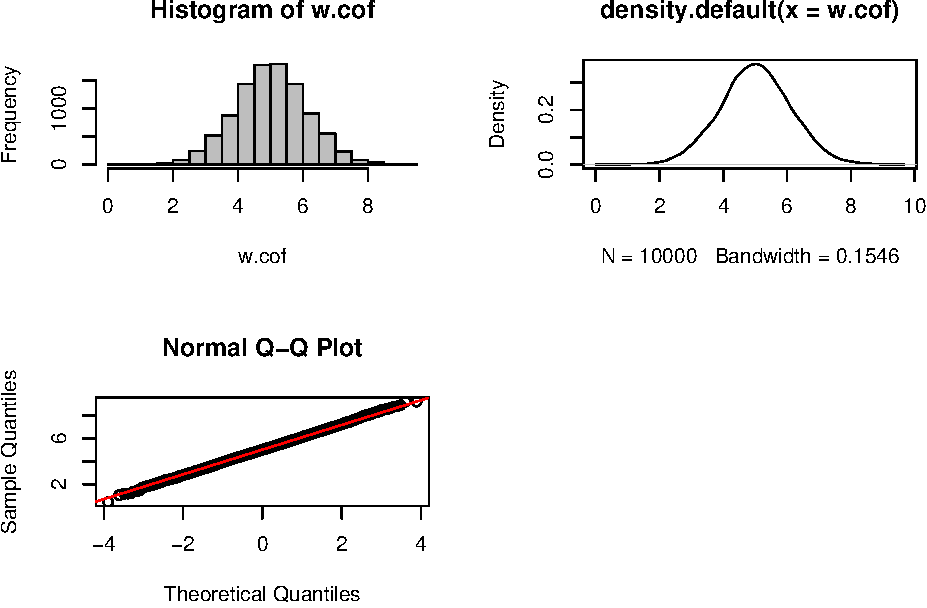
\includegraphics{Managing_batch_effects_files/figure-latex/unnamed-chunk-75-1.pdf}

BMC, ComBat and removeBatchEffect successfully removed batch variation
while preserving treatment variation, but SVD performed poorly.
Percentile normalisation preserved sufficient treatment variation, but
removed less batch effect variation than BMC, ComBat and
removeBatchEffect. Percentile normalisation used percentiles instead of
actual values. This leads to information loss. Moreover, it was designed
for case-control microbiome studies, which differ from our example
studies. This method would therefore be more effective with control
samples in each batch. SVD was inefficient at targeting batch effects,
as it assumes that batch effects cause the largest variation in the data
and should therefore appear as the first component. However, in sponge
data the batch effect is mainly present on the second component as was
shown in PCA sample plots with density, which results in a miscorrection
of batch effects.

We also calculate the variance for AD data.

\begin{Shaded}
\begin{Highlighting}[]
\CommentTok{# AD data}
\NormalTok{ad.form <-}\StringTok{ }\ErrorTok{~}\StringTok{ }\NormalTok{ad.trt }\OperatorTok{+}\StringTok{ }\NormalTok{ad.batch}
\NormalTok{ad.info <-}\StringTok{ }\KeywordTok{as.data.frame}\NormalTok{(}\KeywordTok{cbind}\NormalTok{(}\KeywordTok{rownames}\NormalTok{(ad.clr), ad.trt,ad.batch))}
\KeywordTok{rownames}\NormalTok{(ad.info) <-}\StringTok{ }\KeywordTok{rownames}\NormalTok{(ad.clr)}

\CommentTok{# before}
\NormalTok{ad.varPart.before <-}\StringTok{ }\KeywordTok{fitExtractVarPartModel}\NormalTok{(}\DataTypeTok{exprObj =} \KeywordTok{t}\NormalTok{(ad.clr), }
                                            \DataTypeTok{formula =}\NormalTok{ ad.form, }\DataTypeTok{data =}\NormalTok{ ad.info)}

\CommentTok{# BMC}
\NormalTok{ad.varPart.bmc <-}\StringTok{ }\KeywordTok{fitExtractVarPartModel}\NormalTok{(}\DataTypeTok{exprObj =} \KeywordTok{t}\NormalTok{(ad.bmc), }
                                         \DataTypeTok{formula =}\NormalTok{ ad.form, }\DataTypeTok{data =}\NormalTok{ ad.info)}

\CommentTok{# combat}
\NormalTok{ad.varPart.combat <-}\StringTok{ }\KeywordTok{fitExtractVarPartModel}\NormalTok{(}\DataTypeTok{exprObj =} \KeywordTok{t}\NormalTok{(ad.combat), }
                                            \DataTypeTok{formula =}\NormalTok{ ad.form, }\DataTypeTok{data =}\NormalTok{ ad.info)}

\CommentTok{# removeBatchEffect}
\NormalTok{ad.varPart.limma <-}\StringTok{ }\KeywordTok{fitExtractVarPartModel}\NormalTok{(}\DataTypeTok{exprObj =} \KeywordTok{t}\NormalTok{(ad.limma), }
                                           \DataTypeTok{formula =}\NormalTok{ ad.form, }\DataTypeTok{data =}\NormalTok{ ad.info)}

\CommentTok{# percentile normalisation}
\NormalTok{ad.varPart.percentile <-}\StringTok{ }\KeywordTok{fitExtractVarPartModel}\NormalTok{(}\DataTypeTok{exprObj =} \KeywordTok{t}\NormalTok{(ad.percentile), }
                                                \DataTypeTok{formula =}\NormalTok{ ad.form, }\DataTypeTok{data =}\NormalTok{ ad.info)}

\CommentTok{# svd}
\NormalTok{ad.varPart.svd <-}\StringTok{ }\KeywordTok{fitExtractVarPartModel}\NormalTok{(}\DataTypeTok{exprObj =} \KeywordTok{t}\NormalTok{(ad.svd), }
                                         \DataTypeTok{formula =}\NormalTok{ ad.form, }\DataTypeTok{data =}\NormalTok{ ad.info)}

\CommentTok{# ruv}
\NormalTok{ad.varPart.ruv <-}\StringTok{ }\KeywordTok{fitExtractVarPartModel}\NormalTok{(}\DataTypeTok{exprObj =} \KeywordTok{t}\NormalTok{(ad.ruvIII), }
                                         \DataTypeTok{formula =}\NormalTok{ ad.form, }\DataTypeTok{data =}\NormalTok{ ad.info)}
\end{Highlighting}
\end{Shaded}

\begin{Shaded}
\begin{Highlighting}[]
\CommentTok{# extract the variance of trt and batch}
\CommentTok{# before}
\NormalTok{ad.varmat.before <-}\StringTok{ }\KeywordTok{as.matrix}\NormalTok{(ad.varPart.before[ ,}\DecValTok{1}\OperatorTok{:}\DecValTok{2}\NormalTok{])}
\CommentTok{# BMC}
\NormalTok{ad.varmat.bmc <-}\StringTok{ }\KeywordTok{as.matrix}\NormalTok{(ad.varPart.bmc[ ,}\DecValTok{1}\OperatorTok{:}\DecValTok{2}\NormalTok{])}
\CommentTok{# ComBat}
\NormalTok{ad.varmat.combat <-}\StringTok{ }\KeywordTok{as.matrix}\NormalTok{(ad.varPart.combat[ ,}\DecValTok{1}\OperatorTok{:}\DecValTok{2}\NormalTok{])}
\CommentTok{# removeBatchEffect}
\NormalTok{ad.varmat.limma <-}\StringTok{ }\KeywordTok{as.matrix}\NormalTok{(ad.varPart.limma[ ,}\DecValTok{1}\OperatorTok{:}\DecValTok{2}\NormalTok{])}
\CommentTok{# percentile normalisation}
\NormalTok{ad.varmat.percentile <-}\StringTok{ }\KeywordTok{as.matrix}\NormalTok{(ad.varPart.percentile[ ,}\DecValTok{1}\OperatorTok{:}\DecValTok{2}\NormalTok{])}
\CommentTok{# SVD}
\NormalTok{ad.varmat.svd <-}\StringTok{ }\KeywordTok{as.matrix}\NormalTok{(ad.varPart.svd[ ,}\DecValTok{1}\OperatorTok{:}\DecValTok{2}\NormalTok{])}
\CommentTok{# RUVIII}
\NormalTok{ad.varmat.ruv <-}\StringTok{ }\KeywordTok{as.matrix}\NormalTok{(ad.varPart.ruv[ ,}\DecValTok{1}\OperatorTok{:}\DecValTok{2}\NormalTok{])}


\CommentTok{# merge results}
\NormalTok{ad.variance <-}\StringTok{ }\KeywordTok{c}\NormalTok{(}\KeywordTok{as.vector}\NormalTok{(ad.varmat.before), }\KeywordTok{as.vector}\NormalTok{(ad.varmat.bmc),}
                 \KeywordTok{as.vector}\NormalTok{(ad.varmat.combat), }\KeywordTok{as.vector}\NormalTok{(ad.varmat.limma),}
                 \KeywordTok{as.vector}\NormalTok{(ad.varmat.percentile), }\KeywordTok{as.vector}\NormalTok{(ad.varmat.svd), }
                 \KeywordTok{as.vector}\NormalTok{(ad.varmat.ruv))}

\CommentTok{# add batch, trt and methods info}
\NormalTok{ad.variance <-}\StringTok{ }\KeywordTok{cbind}\NormalTok{(}\DataTypeTok{variance =}\NormalTok{ ad.variance, }
                     \DataTypeTok{Type =} \KeywordTok{rep}\NormalTok{(}\KeywordTok{c}\NormalTok{( }\StringTok{'Treatment'}\NormalTok{, }\StringTok{'Batch'}\NormalTok{), }\DataTypeTok{each =} \KeywordTok{ncol}\NormalTok{(ad.clr)),}
                     \DataTypeTok{method =} \KeywordTok{rep}\NormalTok{(}\KeywordTok{c}\NormalTok{(}\StringTok{'Before'}\NormalTok{, }\StringTok{'BMC'}\NormalTok{, }\StringTok{'ComBat'}\NormalTok{, }\StringTok{'rBE'}\NormalTok{, }\StringTok{'PN'}\NormalTok{, }
                                    \StringTok{'SVD'}\NormalTok{, }\StringTok{'RUVIII'}\NormalTok{), }\DataTypeTok{each =} \DecValTok{2}\OperatorTok{*}\KeywordTok{ncol}\NormalTok{(ad.clr)))}
\CommentTok{# reorder levels  }
\NormalTok{ad.variance <-}\StringTok{ }\KeywordTok{as.data.frame}\NormalTok{(ad.variance)}
\NormalTok{ad.variance}\OperatorTok{$}\NormalTok{method <-}\StringTok{ }\KeywordTok{factor}\NormalTok{(ad.variance}\OperatorTok{$}\NormalTok{method, }
                            \DataTypeTok{levels =} \KeywordTok{unique}\NormalTok{(ad.variance}\OperatorTok{$}\NormalTok{method))}
\NormalTok{ad.variance}\OperatorTok{$}\NormalTok{variance <-}\StringTok{ }\KeywordTok{as.numeric}\NormalTok{(}\KeywordTok{as.character}\NormalTok{(ad.variance}\OperatorTok{$}\NormalTok{variance))}

\KeywordTok{ggplot}\NormalTok{(ad.variance, }\KeywordTok{aes}\NormalTok{(}\DataTypeTok{x =}\NormalTok{ Type, }\DataTypeTok{y =}\NormalTok{ variance, }\DataTypeTok{fill =}\NormalTok{ Type)) }\OperatorTok{+}\StringTok{ }
\StringTok{  }\KeywordTok{geom_boxplot}\NormalTok{() }\OperatorTok{+}\StringTok{ }\KeywordTok{facet_grid}\NormalTok{(}\DataTypeTok{cols =} \KeywordTok{vars}\NormalTok{(method)) }\OperatorTok{+}\StringTok{ }\KeywordTok{theme_bw}\NormalTok{() }\OperatorTok{+}\StringTok{ }
\StringTok{  }\KeywordTok{theme}\NormalTok{(}\DataTypeTok{axis.text.x =} \KeywordTok{element_text}\NormalTok{(}\DataTypeTok{angle =} \DecValTok{60}\NormalTok{, }\DataTypeTok{hjust =} \DecValTok{1}\NormalTok{), }
        \DataTypeTok{strip.text =} \KeywordTok{element_text}\NormalTok{(}\DataTypeTok{size =} \DecValTok{11}\NormalTok{), }\DataTypeTok{panel.grid =} \KeywordTok{element_blank}\NormalTok{(), }
        \DataTypeTok{axis.text =} \KeywordTok{element_text}\NormalTok{(}\DataTypeTok{size =} \DecValTok{12}\NormalTok{), }\DataTypeTok{axis.title =} \KeywordTok{element_text}\NormalTok{(}\DataTypeTok{size =} \DecValTok{15}\NormalTok{),}
        \DataTypeTok{legend.title =} \KeywordTok{element_text}\NormalTok{(}\DataTypeTok{size =} \DecValTok{15}\NormalTok{), }\DataTypeTok{legend.text =} \KeywordTok{element_text}\NormalTok{(}\DataTypeTok{size =} \DecValTok{12}\NormalTok{)) }\OperatorTok{+}\StringTok{ }
\StringTok{  }\KeywordTok{labs}\NormalTok{(}\DataTypeTok{x =} \StringTok{"Type"}\NormalTok{, }\DataTypeTok{y =} \StringTok{"Proportion Variance"}\NormalTok{, }\DataTypeTok{name =} \StringTok{'Type'}\NormalTok{) }\OperatorTok{+}\StringTok{ }
\StringTok{  }\KeywordTok{scale_fill_hue}\NormalTok{(}\DataTypeTok{l =} \DecValTok{40}\NormalTok{) }\OperatorTok{+}\StringTok{ }\KeywordTok{ylim}\NormalTok{(}\DecValTok{0}\NormalTok{,}\DecValTok{1}\NormalTok{)}
\end{Highlighting}
\end{Shaded}

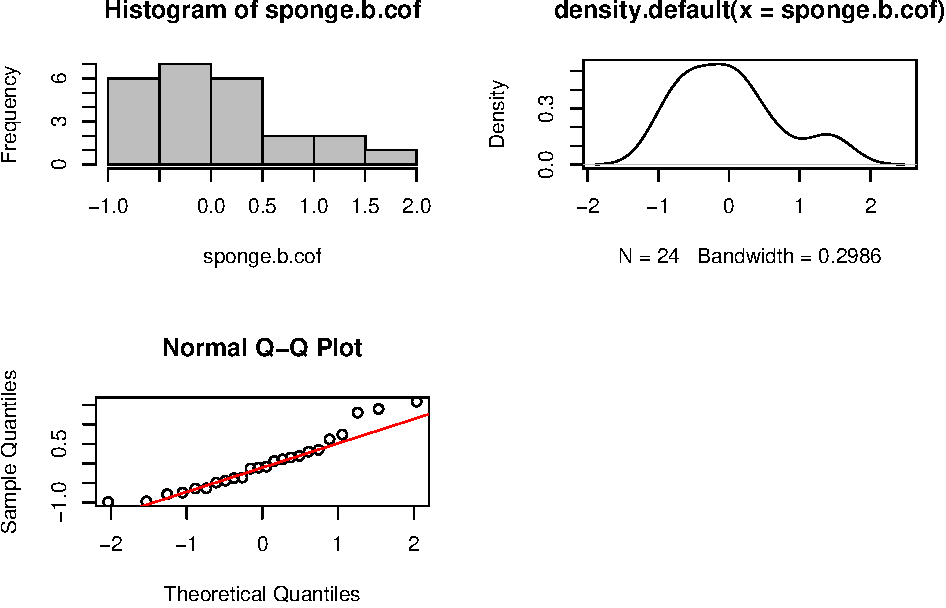
\includegraphics{Managing_batch_effects_files/figure-latex/unnamed-chunk-77-1.pdf}

Similar results as in sponge data, BMC, ComBat and removeBatchEffect
successfully removed batch variation while preserving treatment
variation, but SVD performed poorly. Percentile normalisation and RUVIII
preserved sufficient treatment variation, but removed less batch effect
variation than BMC, ComBat and removeBatchEffect. It is possible the
negative control variables or technical replicate samples did not
entirely capture the batch effects. SVD was also inefficient at
targeting batch effects, as in AD data the batch effect is present on
both first and second components, which results in a miscorrection of
batch effects.

\subsection{RDA}\label{rda}

The pRDA method is a multivariate method to assess \emph{globally} the
effect of batch and treatment (two separate models).

\begin{Shaded}
\begin{Highlighting}[]
\CommentTok{# Sponge data}
\NormalTok{sponge.data.design <-}\StringTok{ }\KeywordTok{numeric}\NormalTok{()}
\NormalTok{sponge.data.design}\OperatorTok{$}\NormalTok{group <-}\StringTok{ }\NormalTok{sponge.trt}
\NormalTok{sponge.data.design}\OperatorTok{$}\NormalTok{batch <-}\StringTok{ }\NormalTok{sponge.batch}

\CommentTok{# before}
\CommentTok{# conditioning on a batch effect}
\NormalTok{sponge.rda.before1 <-}\StringTok{ }\KeywordTok{rda}\NormalTok{(sponge.tss.clr }\OperatorTok{~}\StringTok{ }\NormalTok{group }\OperatorTok{+}\StringTok{ }\KeywordTok{Condition}\NormalTok{(batch), }
                         \DataTypeTok{data =}\NormalTok{ sponge.data.design)}
\NormalTok{sponge.rda.before2 <-}\StringTok{ }\KeywordTok{rda}\NormalTok{(sponge.tss.clr }\OperatorTok{~}\StringTok{ }\NormalTok{batch }\OperatorTok{+}\StringTok{ }\KeywordTok{Condition}\NormalTok{(group), }
                         \DataTypeTok{data =}\NormalTok{ sponge.data.design)}

\CommentTok{# amount of variance}
\NormalTok{sponge.rda.bat_prop.before <-}\StringTok{ }\NormalTok{sponge.rda.before1}\OperatorTok{$}\NormalTok{pCCA}\OperatorTok{$}\NormalTok{tot.chi}\OperatorTok{*}\DecValTok{100}\OperatorTok{/}\NormalTok{sponge.rda.before1}\OperatorTok{$}\NormalTok{tot.chi}
\NormalTok{sponge.rda.trt_prop.before <-}\StringTok{ }\NormalTok{sponge.rda.before2}\OperatorTok{$}\NormalTok{pCCA}\OperatorTok{$}\NormalTok{tot.chi}\OperatorTok{*}\DecValTok{100}\OperatorTok{/}\NormalTok{sponge.rda.before2}\OperatorTok{$}\NormalTok{tot.chi}

\CommentTok{# BMC}
\CommentTok{# conditioning on a batch effect}
\NormalTok{sponge.rda.bmc1 <-}\StringTok{ }\KeywordTok{rda}\NormalTok{(sponge.bmc }\OperatorTok{~}\StringTok{ }\NormalTok{group }\OperatorTok{+}\StringTok{ }\KeywordTok{Condition}\NormalTok{(batch), }
                      \DataTypeTok{data =}\NormalTok{ sponge.data.design)}
\NormalTok{sponge.rda.bmc2 <-}\StringTok{ }\KeywordTok{rda}\NormalTok{(sponge.bmc }\OperatorTok{~}\StringTok{ }\NormalTok{batch }\OperatorTok{+}\StringTok{ }\KeywordTok{Condition}\NormalTok{(group), }
                      \DataTypeTok{data =}\NormalTok{ sponge.data.design)}

\CommentTok{# amount of variance}
\NormalTok{sponge.rda.bat_prop.bmc <-}\StringTok{ }\NormalTok{sponge.rda.bmc1}\OperatorTok{$}\NormalTok{pCCA}\OperatorTok{$}\NormalTok{tot.chi}\OperatorTok{*}\DecValTok{100}\OperatorTok{/}\NormalTok{sponge.rda.bmc1}\OperatorTok{$}\NormalTok{tot.chi}
\NormalTok{sponge.rda.trt_prop.bmc <-}\StringTok{ }\NormalTok{sponge.rda.bmc2}\OperatorTok{$}\NormalTok{pCCA}\OperatorTok{$}\NormalTok{tot.chi}\OperatorTok{*}\DecValTok{100}\OperatorTok{/}\NormalTok{sponge.rda.bmc2}\OperatorTok{$}\NormalTok{tot.chi}


\CommentTok{# combat}
\CommentTok{# conditioning on a batch effect}
\NormalTok{sponge.rda.combat1 <-}\StringTok{ }\KeywordTok{rda}\NormalTok{(sponge.combat }\OperatorTok{~}\StringTok{ }\NormalTok{group }\OperatorTok{+}\StringTok{ }\KeywordTok{Condition}\NormalTok{(batch), }
                         \DataTypeTok{data =}\NormalTok{ sponge.data.design)}
\NormalTok{sponge.rda.combat2 <-}\StringTok{ }\KeywordTok{rda}\NormalTok{(sponge.combat }\OperatorTok{~}\StringTok{ }\NormalTok{batch }\OperatorTok{+}\StringTok{ }\KeywordTok{Condition}\NormalTok{(group), }
                         \DataTypeTok{data =}\NormalTok{ sponge.data.design)}

\CommentTok{# amount of variance}
\NormalTok{sponge.rda.bat_prop.combat <-}\StringTok{ }\NormalTok{sponge.rda.combat1}\OperatorTok{$}\NormalTok{pCCA}\OperatorTok{$}\NormalTok{tot.chi}\OperatorTok{*}\DecValTok{100}\OperatorTok{/}\NormalTok{sponge.rda.combat1}\OperatorTok{$}\NormalTok{tot.chi}
\NormalTok{sponge.rda.trt_prop.combat <-}\StringTok{ }\NormalTok{sponge.rda.combat2}\OperatorTok{$}\NormalTok{pCCA}\OperatorTok{$}\NormalTok{tot.chi}\OperatorTok{*}\DecValTok{100}\OperatorTok{/}\NormalTok{sponge.rda.combat2}\OperatorTok{$}\NormalTok{tot.chi}


\CommentTok{# limma}
\CommentTok{# conditioning on a batch effect}
\NormalTok{sponge.rda.limma1 <-}\StringTok{ }\KeywordTok{rda}\NormalTok{(sponge.limma }\OperatorTok{~}\StringTok{ }\NormalTok{group }\OperatorTok{+}\StringTok{ }\KeywordTok{Condition}\NormalTok{(batch), }
                        \DataTypeTok{data =}\NormalTok{ sponge.data.design)}
\NormalTok{sponge.rda.limma2 <-}\StringTok{ }\KeywordTok{rda}\NormalTok{(sponge.limma }\OperatorTok{~}\StringTok{ }\NormalTok{batch }\OperatorTok{+}\StringTok{ }\KeywordTok{Condition}\NormalTok{(group), }
                        \DataTypeTok{data =}\NormalTok{ sponge.data.design)}

\CommentTok{# amount of variance}
\NormalTok{sponge.rda.bat_prop.limma <-}\StringTok{ }\NormalTok{sponge.rda.limma1}\OperatorTok{$}\NormalTok{pCCA}\OperatorTok{$}\NormalTok{tot.chi}\OperatorTok{*}\DecValTok{100}\OperatorTok{/}\NormalTok{sponge.rda.limma1}\OperatorTok{$}\NormalTok{tot.chi}
\NormalTok{sponge.rda.trt_prop.limma <-}\StringTok{ }\NormalTok{sponge.rda.limma2}\OperatorTok{$}\NormalTok{pCCA}\OperatorTok{$}\NormalTok{tot.chi}\OperatorTok{*}\DecValTok{100}\OperatorTok{/}\NormalTok{sponge.rda.limma2}\OperatorTok{$}\NormalTok{tot.chi}


\CommentTok{# percentile}
\CommentTok{# conditioning on a batch effect}
\NormalTok{sponge.rda.percentile1 <-}\StringTok{ }\KeywordTok{rda}\NormalTok{(sponge.percentile }\OperatorTok{~}\StringTok{ }\NormalTok{group }\OperatorTok{+}\StringTok{ }\KeywordTok{Condition}\NormalTok{(batch), }
                             \DataTypeTok{data =}\NormalTok{ sponge.data.design)}
\NormalTok{sponge.rda.percentile2 <-}\StringTok{ }\KeywordTok{rda}\NormalTok{(sponge.percentile }\OperatorTok{~}\StringTok{ }\NormalTok{batch }\OperatorTok{+}\StringTok{ }\KeywordTok{Condition}\NormalTok{(group), }
                             \DataTypeTok{data =}\NormalTok{ sponge.data.design)}

\CommentTok{# amount of variance}
\NormalTok{sponge.rda.bat_prop.percentile <-}\StringTok{ }\NormalTok{sponge.rda.percentile1}\OperatorTok{$}\NormalTok{pCCA}\OperatorTok{$}\NormalTok{tot.chi}\OperatorTok{*}\DecValTok{100}\OperatorTok{/}\NormalTok{sponge.rda.percentile1}\OperatorTok{$}\NormalTok{tot.chi}
\NormalTok{sponge.rda.trt_prop.percentile <-}\StringTok{ }\NormalTok{sponge.rda.percentile2}\OperatorTok{$}\NormalTok{pCCA}\OperatorTok{$}\NormalTok{tot.chi}\OperatorTok{*}\DecValTok{100}\OperatorTok{/}\NormalTok{sponge.rda.percentile2}\OperatorTok{$}\NormalTok{tot.chi}


\CommentTok{# SVD}
\CommentTok{# conditioning on a batch effect}
\NormalTok{sponge.rda.svd1 <-}\StringTok{ }\KeywordTok{rda}\NormalTok{(sponge.svd }\OperatorTok{~}\StringTok{ }\NormalTok{group }\OperatorTok{+}\StringTok{ }\KeywordTok{Condition}\NormalTok{(batch), }
                      \DataTypeTok{data =}\NormalTok{ sponge.data.design)}
\NormalTok{sponge.rda.svd2 <-}\StringTok{ }\KeywordTok{rda}\NormalTok{(sponge.svd }\OperatorTok{~}\StringTok{ }\NormalTok{batch }\OperatorTok{+}\StringTok{ }\KeywordTok{Condition}\NormalTok{(group), }
                      \DataTypeTok{data =}\NormalTok{ sponge.data.design)}

\CommentTok{# amount of variance}
\NormalTok{sponge.rda.bat_prop.svd <-}\StringTok{ }\NormalTok{sponge.rda.svd1}\OperatorTok{$}\NormalTok{pCCA}\OperatorTok{$}\NormalTok{tot.chi}\OperatorTok{*}\DecValTok{100}\OperatorTok{/}\NormalTok{sponge.rda.svd1}\OperatorTok{$}\NormalTok{tot.chi}
\NormalTok{sponge.rda.trt_prop.svd <-}\StringTok{ }\NormalTok{sponge.rda.svd2}\OperatorTok{$}\NormalTok{pCCA}\OperatorTok{$}\NormalTok{tot.chi}\OperatorTok{*}\DecValTok{100}\OperatorTok{/}\NormalTok{sponge.rda.svd2}\OperatorTok{$}\NormalTok{tot.chi}
\end{Highlighting}
\end{Shaded}

We now represent the amount of variance explained by batch and treatment
estimated with pRDA:

\begin{Shaded}
\begin{Highlighting}[]
\CommentTok{# proportion}
\NormalTok{sponge.rda.prop.before <-}\StringTok{ }\KeywordTok{c}\NormalTok{(sponge.rda.bat_prop.before, }
\NormalTok{                           sponge.rda.trt_prop.before)}
\NormalTok{sponge.rda.prop.bmc <-}\StringTok{ }\KeywordTok{c}\NormalTok{(sponge.rda.bat_prop.bmc, }
\NormalTok{                        sponge.rda.trt_prop.bmc)}
\NormalTok{sponge.rda.prop.combat <-}\StringTok{ }\KeywordTok{c}\NormalTok{(sponge.rda.bat_prop.combat, }
\NormalTok{                           sponge.rda.trt_prop.combat)}
\NormalTok{sponge.rda.prop.limma <-}\StringTok{ }\KeywordTok{c}\NormalTok{(sponge.rda.bat_prop.limma, }
\NormalTok{                          sponge.rda.trt_prop.limma)}
\NormalTok{sponge.rda.prop.percentile <-}\StringTok{ }\KeywordTok{c}\NormalTok{(sponge.rda.bat_prop.percentile, }
\NormalTok{                               sponge.rda.trt_prop.percentile)}
\NormalTok{sponge.rda.prop.svd <-}\StringTok{ }\KeywordTok{c}\NormalTok{(sponge.rda.bat_prop.svd, }
\NormalTok{                        sponge.rda.trt_prop.svd)}

\CommentTok{# merge results}
\NormalTok{sponge.rda.prop.val <-}\StringTok{ }\KeywordTok{c}\NormalTok{(sponge.rda.prop.before, sponge.rda.prop.bmc, }
\NormalTok{                        sponge.rda.prop.combat, sponge.rda.prop.limma, }
\NormalTok{                        sponge.rda.prop.percentile, sponge.rda.prop.svd)}

\CommentTok{# add batch, trt and method info}
\NormalTok{sponge.rda.prop <-}\StringTok{ }\KeywordTok{data.frame}\NormalTok{(}\DataTypeTok{prop =}\NormalTok{ sponge.rda.prop.val, }
                             \DataTypeTok{prop.r =} \KeywordTok{round}\NormalTok{(sponge.rda.prop.val, }\DecValTok{2}\NormalTok{), }
                             \DataTypeTok{Method =} \KeywordTok{rep}\NormalTok{(}\KeywordTok{c}\NormalTok{(}\StringTok{'Before'}\NormalTok{, }\StringTok{'BMC'}\NormalTok{, }\StringTok{'ComBat'}\NormalTok{, }
                                            \StringTok{'rBE'}\NormalTok{, }\StringTok{'PN'}\NormalTok{, }\StringTok{'SVD'}\NormalTok{), }\DataTypeTok{each =} \DecValTok{2}\NormalTok{), }
                             \DataTypeTok{Type =} \KeywordTok{rep}\NormalTok{(}\KeywordTok{c}\NormalTok{(}\StringTok{'Batch'}\NormalTok{, }\StringTok{'Tissue'}\NormalTok{), }\DecValTok{6}\NormalTok{))}

\CommentTok{# reorder levels}
\NormalTok{sponge.rda.prop}\OperatorTok{$}\NormalTok{Method <-}\StringTok{ }\KeywordTok{factor}\NormalTok{(sponge.rda.prop}\OperatorTok{$}\NormalTok{Method, }
                                \DataTypeTok{levels =} \KeywordTok{unique}\NormalTok{(sponge.rda.prop}\OperatorTok{$}\NormalTok{Method))}

\KeywordTok{ggplot}\NormalTok{(}\DataTypeTok{data =}\NormalTok{ sponge.rda.prop, }\KeywordTok{aes}\NormalTok{(}\DataTypeTok{x =}\NormalTok{ Method, }\DataTypeTok{y =}\NormalTok{ prop, }\DataTypeTok{fill =}\NormalTok{ Type)) }\OperatorTok{+}\StringTok{ }
\StringTok{  }\KeywordTok{geom_bar}\NormalTok{(}\DataTypeTok{stat =} \StringTok{"identity"}\NormalTok{, }\DataTypeTok{position =} \StringTok{'dodge'}\NormalTok{, }\DataTypeTok{colour =} \StringTok{'black'}\NormalTok{) }\OperatorTok{+}\StringTok{ }
\StringTok{  }\KeywordTok{geom_text}\NormalTok{(}\DataTypeTok{data =}\NormalTok{ sponge.rda.prop, }\KeywordTok{aes}\NormalTok{(Method, prop }\OperatorTok{+}\StringTok{ }\FloatTok{2.5}\NormalTok{, }\DataTypeTok{label =}\NormalTok{ prop.r), }
            \DataTypeTok{position =} \KeywordTok{position_dodge}\NormalTok{(}\DataTypeTok{width =} \FloatTok{0.9}\NormalTok{), }\DataTypeTok{size =} \DecValTok{3}\NormalTok{) }\OperatorTok{+}\StringTok{ }\KeywordTok{theme_bw}\NormalTok{() }\OperatorTok{+}\StringTok{ }
\StringTok{  }\KeywordTok{labs}\NormalTok{(}\DataTypeTok{y =} \StringTok{"Variance explained (%)"}\NormalTok{) }\OperatorTok{+}\StringTok{ }
\StringTok{  }\KeywordTok{theme}\NormalTok{(}\DataTypeTok{axis.text.x =} \KeywordTok{element_text}\NormalTok{(}\DataTypeTok{angle =} \DecValTok{60}\NormalTok{, }\DataTypeTok{hjust =} \DecValTok{1}\NormalTok{), }
        \DataTypeTok{panel.grid =} \KeywordTok{element_blank}\NormalTok{(), }\DataTypeTok{axis.text =} \KeywordTok{element_text}\NormalTok{(}\DataTypeTok{size =} \DecValTok{12}\NormalTok{), }
        \DataTypeTok{axis.title =} \KeywordTok{element_text}\NormalTok{(}\DataTypeTok{size =} \DecValTok{15}\NormalTok{), }\DataTypeTok{legend.title =} \KeywordTok{element_text}\NormalTok{(}\DataTypeTok{size =} \DecValTok{15}\NormalTok{),}
        \DataTypeTok{legend.text =} \KeywordTok{element_text}\NormalTok{(}\DataTypeTok{size =} \DecValTok{12}\NormalTok{)) }\OperatorTok{+}\StringTok{ }\KeywordTok{ylim}\NormalTok{(}\DecValTok{0}\NormalTok{,}\DecValTok{100}\NormalTok{)}
\end{Highlighting}
\end{Shaded}

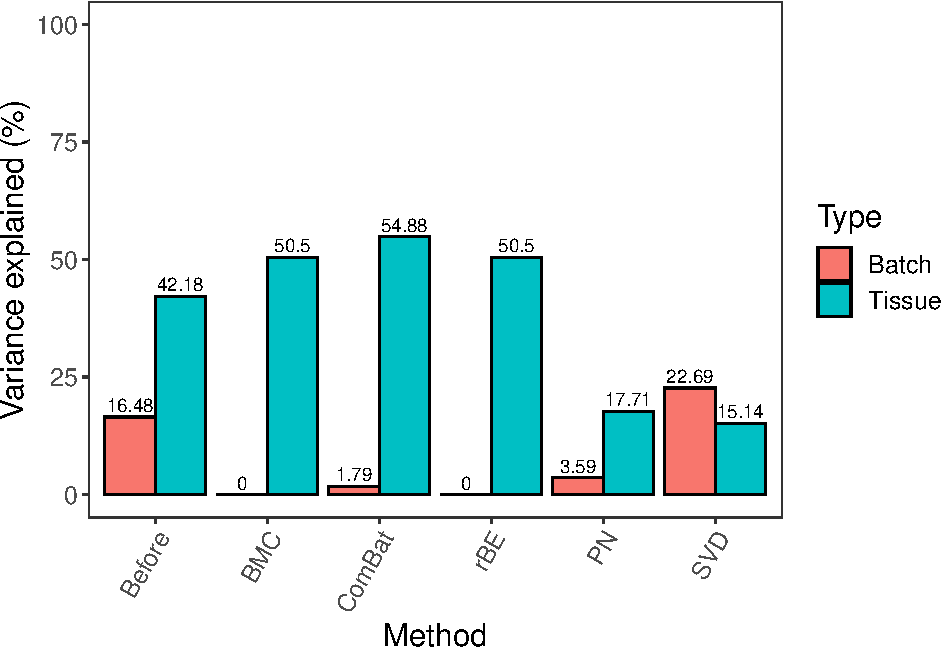
\includegraphics{Managing_batch_effects_files/figure-latex/unnamed-chunk-79-1.pdf}

In sponge data, pRDA shows that BMC, ComBat and removeBatchEffect were
more efficient at removing batch variation while preserving treatment
variation. This result is in agreement with the proportional variance
calculated using a linear model in the previous section `linear model
per variable'. ComBat removed relatively less batch variation compared
with the other two methods, which implies that the batch effect is not
purely systematic. The low efficiency of percentile normalisation is
more obvious in the variance calculated with pRDA. It did not remove
enough batch variation, nor preserve enough treatment variation in
sponge data.

We also apply pRDA on AD data.

\begin{Shaded}
\begin{Highlighting}[]
\CommentTok{# AD data}
\NormalTok{ad.data.design <-}\StringTok{ }\KeywordTok{numeric}\NormalTok{()}
\NormalTok{ad.data.design}\OperatorTok{$}\NormalTok{group <-}\StringTok{ }\NormalTok{ad.trt}
\NormalTok{ad.data.design}\OperatorTok{$}\NormalTok{batch <-}\StringTok{ }\NormalTok{ad.batch}

\CommentTok{# before}
\CommentTok{# conditioning on a batch effect}
\NormalTok{ad.rda.before1 <-}\StringTok{ }\KeywordTok{rda}\NormalTok{(ad.clr }\OperatorTok{~}\StringTok{ }\NormalTok{group }\OperatorTok{+}\StringTok{ }\KeywordTok{Condition}\NormalTok{(batch), }\DataTypeTok{data =}\NormalTok{ ad.data.design)}
\NormalTok{ad.rda.before2 <-}\StringTok{ }\KeywordTok{rda}\NormalTok{(ad.clr }\OperatorTok{~}\StringTok{ }\NormalTok{batch }\OperatorTok{+}\StringTok{ }\KeywordTok{Condition}\NormalTok{(group), }\DataTypeTok{data =}\NormalTok{ ad.data.design)}

\CommentTok{# amount of variance}
\NormalTok{ad.rda.bat_prop.before <-}\StringTok{ }\NormalTok{ad.rda.before1}\OperatorTok{$}\NormalTok{pCCA}\OperatorTok{$}\NormalTok{tot.chi}\OperatorTok{*}\DecValTok{100}\OperatorTok{/}\NormalTok{ad.rda.before1}\OperatorTok{$}\NormalTok{tot.chi}
\NormalTok{ad.rda.trt_prop.before <-}\StringTok{ }\NormalTok{ad.rda.before2}\OperatorTok{$}\NormalTok{pCCA}\OperatorTok{$}\NormalTok{tot.chi}\OperatorTok{*}\DecValTok{100}\OperatorTok{/}\NormalTok{ad.rda.before2}\OperatorTok{$}\NormalTok{tot.chi}

\CommentTok{# BMC}
\CommentTok{# conditioning on a batch effect}
\NormalTok{ad.rda.bmc1 <-}\StringTok{ }\KeywordTok{rda}\NormalTok{(ad.bmc }\OperatorTok{~}\StringTok{ }\NormalTok{group }\OperatorTok{+}\StringTok{ }\KeywordTok{Condition}\NormalTok{(batch), }\DataTypeTok{data =}\NormalTok{ ad.data.design)}
\NormalTok{ad.rda.bmc2 <-}\StringTok{ }\KeywordTok{rda}\NormalTok{(ad.bmc }\OperatorTok{~}\StringTok{ }\NormalTok{batch }\OperatorTok{+}\StringTok{ }\KeywordTok{Condition}\NormalTok{(group), }\DataTypeTok{data =}\NormalTok{ ad.data.design)}

\CommentTok{# amount of variance}
\NormalTok{ad.rda.bat_prop.bmc <-}\StringTok{ }\NormalTok{ad.rda.bmc1}\OperatorTok{$}\NormalTok{pCCA}\OperatorTok{$}\NormalTok{tot.chi}\OperatorTok{*}\DecValTok{100}\OperatorTok{/}\NormalTok{ad.rda.bmc1}\OperatorTok{$}\NormalTok{tot.chi}
\NormalTok{ad.rda.trt_prop.bmc <-}\StringTok{ }\NormalTok{ad.rda.bmc2}\OperatorTok{$}\NormalTok{pCCA}\OperatorTok{$}\NormalTok{tot.chi}\OperatorTok{*}\DecValTok{100}\OperatorTok{/}\NormalTok{ad.rda.bmc2}\OperatorTok{$}\NormalTok{tot.chi}


\CommentTok{# combat}
\CommentTok{# conditioning on a batch effect}
\NormalTok{ad.rda.combat1 <-}\StringTok{ }\KeywordTok{rda}\NormalTok{(ad.combat }\OperatorTok{~}\StringTok{ }\NormalTok{group }\OperatorTok{+}\StringTok{ }\KeywordTok{Condition}\NormalTok{(batch), }\DataTypeTok{data =}\NormalTok{ ad.data.design)}
\NormalTok{ad.rda.combat2 <-}\StringTok{ }\KeywordTok{rda}\NormalTok{(ad.combat }\OperatorTok{~}\StringTok{ }\NormalTok{batch }\OperatorTok{+}\StringTok{ }\KeywordTok{Condition}\NormalTok{(group), }\DataTypeTok{data =}\NormalTok{ ad.data.design)}

\CommentTok{# amount of variance}
\NormalTok{ad.rda.bat_prop.combat <-}\StringTok{ }\NormalTok{ad.rda.combat1}\OperatorTok{$}\NormalTok{pCCA}\OperatorTok{$}\NormalTok{tot.chi}\OperatorTok{*}\DecValTok{100}\OperatorTok{/}\NormalTok{ad.rda.combat1}\OperatorTok{$}\NormalTok{tot.chi}
\NormalTok{ad.rda.trt_prop.combat <-}\StringTok{ }\NormalTok{ad.rda.combat2}\OperatorTok{$}\NormalTok{pCCA}\OperatorTok{$}\NormalTok{tot.chi}\OperatorTok{*}\DecValTok{100}\OperatorTok{/}\NormalTok{ad.rda.combat2}\OperatorTok{$}\NormalTok{tot.chi}


\CommentTok{# limma}
\CommentTok{# conditioning on a batch effect}
\NormalTok{ad.rda.limma1 <-}\StringTok{ }\KeywordTok{rda}\NormalTok{(ad.limma }\OperatorTok{~}\StringTok{ }\NormalTok{group }\OperatorTok{+}\StringTok{ }\KeywordTok{Condition}\NormalTok{(batch), }\DataTypeTok{data =}\NormalTok{ ad.data.design)}
\NormalTok{ad.rda.limma2 <-}\StringTok{ }\KeywordTok{rda}\NormalTok{(ad.limma }\OperatorTok{~}\StringTok{ }\NormalTok{batch }\OperatorTok{+}\StringTok{ }\KeywordTok{Condition}\NormalTok{(group), }\DataTypeTok{data =}\NormalTok{ ad.data.design)}

\CommentTok{# amount of variance}
\NormalTok{ad.rda.bat_prop.limma <-}\StringTok{ }\NormalTok{ad.rda.limma1}\OperatorTok{$}\NormalTok{pCCA}\OperatorTok{$}\NormalTok{tot.chi}\OperatorTok{*}\DecValTok{100}\OperatorTok{/}\NormalTok{ad.rda.limma1}\OperatorTok{$}\NormalTok{tot.chi}
\NormalTok{ad.rda.trt_prop.limma <-}\StringTok{ }\NormalTok{ad.rda.limma2}\OperatorTok{$}\NormalTok{pCCA}\OperatorTok{$}\NormalTok{tot.chi}\OperatorTok{*}\DecValTok{100}\OperatorTok{/}\NormalTok{ad.rda.limma2}\OperatorTok{$}\NormalTok{tot.chi}


\CommentTok{# percentile}
\CommentTok{# conditioning on a batch effect}
\NormalTok{ad.rda.percentile1 <-}\StringTok{ }\KeywordTok{rda}\NormalTok{(ad.percentile }\OperatorTok{~}\StringTok{ }\NormalTok{group }\OperatorTok{+}\StringTok{ }\KeywordTok{Condition}\NormalTok{(batch), }
                         \DataTypeTok{data =}\NormalTok{ ad.data.design)}
\NormalTok{ad.rda.percentile2 <-}\StringTok{ }\KeywordTok{rda}\NormalTok{(ad.percentile }\OperatorTok{~}\StringTok{ }\NormalTok{batch }\OperatorTok{+}\StringTok{ }\KeywordTok{Condition}\NormalTok{(group), }
                         \DataTypeTok{data =}\NormalTok{ ad.data.design)}

\CommentTok{# amount of variance}
\NormalTok{ad.rda.bat_prop.percentile <-}\StringTok{ }\NormalTok{ad.rda.percentile1}\OperatorTok{$}\NormalTok{pCCA}\OperatorTok{$}\NormalTok{tot.chi}\OperatorTok{*}\DecValTok{100}\OperatorTok{/}\NormalTok{ad.rda.percentile1}\OperatorTok{$}\NormalTok{tot.chi}
\NormalTok{ad.rda.trt_prop.percentile <-}\StringTok{ }\NormalTok{ad.rda.percentile2}\OperatorTok{$}\NormalTok{pCCA}\OperatorTok{$}\NormalTok{tot.chi}\OperatorTok{*}\DecValTok{100}\OperatorTok{/}\NormalTok{ad.rda.percentile2}\OperatorTok{$}\NormalTok{tot.chi}


\CommentTok{# SVD}
\CommentTok{# conditioning on a batch effect}
\NormalTok{ad.rda.svd1 <-}\StringTok{ }\KeywordTok{rda}\NormalTok{(ad.svd }\OperatorTok{~}\StringTok{ }\NormalTok{group }\OperatorTok{+}\StringTok{ }\KeywordTok{Condition}\NormalTok{(batch), }\DataTypeTok{data =}\NormalTok{ ad.data.design)}
\NormalTok{ad.rda.svd2 <-}\StringTok{ }\KeywordTok{rda}\NormalTok{(ad.svd }\OperatorTok{~}\StringTok{ }\NormalTok{batch }\OperatorTok{+}\StringTok{ }\KeywordTok{Condition}\NormalTok{(group), }\DataTypeTok{data =}\NormalTok{ ad.data.design)}

\CommentTok{# amount of variance}
\NormalTok{ad.rda.bat_prop.svd <-}\StringTok{ }\NormalTok{ad.rda.svd1}\OperatorTok{$}\NormalTok{pCCA}\OperatorTok{$}\NormalTok{tot.chi}\OperatorTok{*}\DecValTok{100}\OperatorTok{/}\NormalTok{ad.rda.svd1}\OperatorTok{$}\NormalTok{tot.chi}
\NormalTok{ad.rda.trt_prop.svd <-}\StringTok{ }\NormalTok{ad.rda.svd2}\OperatorTok{$}\NormalTok{pCCA}\OperatorTok{$}\NormalTok{tot.chi}\OperatorTok{*}\DecValTok{100}\OperatorTok{/}\NormalTok{ad.rda.svd2}\OperatorTok{$}\NormalTok{tot.chi}


\CommentTok{# RUVIII}
\CommentTok{# conditioning on a batch effect}
\NormalTok{ad.rda.ruv1 <-}\StringTok{ }\KeywordTok{rda}\NormalTok{(ad.ruvIII }\OperatorTok{~}\StringTok{ }\NormalTok{group }\OperatorTok{+}\StringTok{ }\KeywordTok{Condition}\NormalTok{(batch), }\DataTypeTok{data =}\NormalTok{ ad.data.design)}
\NormalTok{ad.rda.ruv2 <-}\StringTok{ }\KeywordTok{rda}\NormalTok{(ad.ruvIII }\OperatorTok{~}\StringTok{ }\NormalTok{batch }\OperatorTok{+}\StringTok{ }\KeywordTok{Condition}\NormalTok{(group), }\DataTypeTok{data =}\NormalTok{ ad.data.design)}

\CommentTok{# amount of variance}
\NormalTok{ad.rda.bat_prop.ruv <-}\StringTok{ }\NormalTok{ad.rda.ruv1}\OperatorTok{$}\NormalTok{pCCA}\OperatorTok{$}\NormalTok{tot.chi}\OperatorTok{*}\DecValTok{100}\OperatorTok{/}\NormalTok{ad.rda.ruv1}\OperatorTok{$}\NormalTok{tot.chi}
\NormalTok{ad.rda.trt_prop.ruv <-}\StringTok{ }\NormalTok{ad.rda.ruv2}\OperatorTok{$}\NormalTok{pCCA}\OperatorTok{$}\NormalTok{tot.chi}\OperatorTok{*}\DecValTok{100}\OperatorTok{/}\NormalTok{ad.rda.ruv2}\OperatorTok{$}\NormalTok{tot.chi}
\end{Highlighting}
\end{Shaded}

\begin{Shaded}
\begin{Highlighting}[]
\CommentTok{# proportion}
\NormalTok{ad.rda.prop.before <-}\StringTok{ }\KeywordTok{c}\NormalTok{(ad.rda.bat_prop.before, ad.rda.trt_prop.before)}
\NormalTok{ad.rda.prop.bmc <-}\StringTok{ }\KeywordTok{c}\NormalTok{(ad.rda.bat_prop.bmc, ad.rda.trt_prop.bmc)}
\NormalTok{ad.rda.prop.combat <-}\StringTok{ }\KeywordTok{c}\NormalTok{(ad.rda.bat_prop.combat, ad.rda.trt_prop.combat)}
\NormalTok{ad.rda.prop.limma <-}\StringTok{ }\KeywordTok{c}\NormalTok{(ad.rda.bat_prop.limma, ad.rda.trt_prop.limma)}
\NormalTok{ad.rda.prop.percentile <-}\StringTok{ }\KeywordTok{c}\NormalTok{(ad.rda.bat_prop.percentile, ad.rda.trt_prop.percentile)}
\NormalTok{ad.rda.prop.svd <-}\StringTok{ }\KeywordTok{c}\NormalTok{(ad.rda.bat_prop.svd, ad.rda.trt_prop.svd)}
\NormalTok{ad.rda.prop.ruv <-}\StringTok{ }\KeywordTok{c}\NormalTok{(ad.rda.bat_prop.ruv, ad.rda.trt_prop.ruv)}

\CommentTok{# merge results}
\NormalTok{ad.rda.prop.val <-}\StringTok{ }\KeywordTok{c}\NormalTok{(ad.rda.prop.before, ad.rda.prop.bmc, }
\NormalTok{                    ad.rda.prop.combat, ad.rda.prop.limma, }
\NormalTok{                    ad.rda.prop.percentile, ad.rda.prop.svd, }
\NormalTok{                    ad.rda.prop.ruv)}

\CommentTok{# add batch, trt and method info}
\NormalTok{ad.rda.prop <-}\StringTok{ }\KeywordTok{data.frame}\NormalTok{(}\DataTypeTok{prop =}\NormalTok{ ad.rda.prop.val, }\DataTypeTok{prop.r =} \KeywordTok{round}\NormalTok{(ad.rda.prop.val, }\DecValTok{2}\NormalTok{), }
                         \DataTypeTok{Method =} \KeywordTok{rep}\NormalTok{(}\KeywordTok{c}\NormalTok{(}\StringTok{'Before'}\NormalTok{, }\StringTok{'BMC'}\NormalTok{, }\StringTok{'ComBat'}\NormalTok{, }\StringTok{'rBE'}\NormalTok{, }
                                        \StringTok{'PN'}\NormalTok{, }\StringTok{'SVD'}\NormalTok{, }\StringTok{'RUVIII'}\NormalTok{), }\DataTypeTok{each =} \DecValTok{2}\NormalTok{), }
                         \DataTypeTok{Type =} \KeywordTok{rep}\NormalTok{(}\KeywordTok{c}\NormalTok{(}\StringTok{'Batch'}\NormalTok{, }\StringTok{'Treatment'}\NormalTok{), }\DecValTok{7}\NormalTok{))}

\CommentTok{# reorder levels}
\NormalTok{ad.rda.prop}\OperatorTok{$}\NormalTok{Method <-}\StringTok{ }\KeywordTok{factor}\NormalTok{(ad.rda.prop}\OperatorTok{$}\NormalTok{Method, }\DataTypeTok{levels =} \KeywordTok{unique}\NormalTok{(ad.rda.prop}\OperatorTok{$}\NormalTok{Method))}

\KeywordTok{ggplot}\NormalTok{(}\DataTypeTok{data =}\NormalTok{ ad.rda.prop, }\KeywordTok{aes}\NormalTok{(}\DataTypeTok{x =}\NormalTok{ Method, }\DataTypeTok{y =}\NormalTok{ prop, }\DataTypeTok{fill =}\NormalTok{ Type)) }\OperatorTok{+}\StringTok{ }
\StringTok{  }\KeywordTok{geom_bar}\NormalTok{(}\DataTypeTok{stat =} \StringTok{"identity"}\NormalTok{, }\DataTypeTok{position =} \StringTok{'dodge'}\NormalTok{, }\DataTypeTok{colour =} \StringTok{'black'}\NormalTok{) }\OperatorTok{+}\StringTok{ }
\StringTok{  }\KeywordTok{geom_text}\NormalTok{(}\DataTypeTok{data =}\NormalTok{ ad.rda.prop, }\KeywordTok{aes}\NormalTok{(Method, prop }\OperatorTok{+}\StringTok{ }\FloatTok{2.5}\NormalTok{, }\DataTypeTok{label =}\NormalTok{ prop.r), }
            \DataTypeTok{position =} \KeywordTok{position_dodge}\NormalTok{(}\DataTypeTok{width =} \DecValTok{1}\NormalTok{), }\DataTypeTok{size =} \DecValTok{3}\NormalTok{) }\OperatorTok{+}\StringTok{ }\KeywordTok{theme_bw}\NormalTok{() }\OperatorTok{+}\StringTok{ }
\StringTok{  }\KeywordTok{labs}\NormalTok{(}\DataTypeTok{y =} \StringTok{"Variance explained (%)"}\NormalTok{) }\OperatorTok{+}\StringTok{ }
\StringTok{  }\KeywordTok{theme}\NormalTok{(}\DataTypeTok{axis.text.x =} \KeywordTok{element_text}\NormalTok{(}\DataTypeTok{angle =} \DecValTok{60}\NormalTok{, }\DataTypeTok{hjust =} \DecValTok{1}\NormalTok{), }
        \DataTypeTok{panel.grid =} \KeywordTok{element_blank}\NormalTok{(), }\DataTypeTok{axis.text =} \KeywordTok{element_text}\NormalTok{(}\DataTypeTok{size =} \DecValTok{12}\NormalTok{), }
        \DataTypeTok{axis.title =} \KeywordTok{element_text}\NormalTok{(}\DataTypeTok{size =} \DecValTok{15}\NormalTok{), }\DataTypeTok{legend.title =} \KeywordTok{element_text}\NormalTok{(}\DataTypeTok{size =} \DecValTok{15}\NormalTok{), }
        \DataTypeTok{legend.text =} \KeywordTok{element_text}\NormalTok{(}\DataTypeTok{size =} \DecValTok{12}\NormalTok{)) }\OperatorTok{+}\StringTok{ }\KeywordTok{scale_fill_hue}\NormalTok{(}\DataTypeTok{l =} \DecValTok{40}\NormalTok{) }\OperatorTok{+}\StringTok{ }\KeywordTok{ylim}\NormalTok{(}\DecValTok{0}\NormalTok{,}\DecValTok{100}\NormalTok{)}
\end{Highlighting}
\end{Shaded}

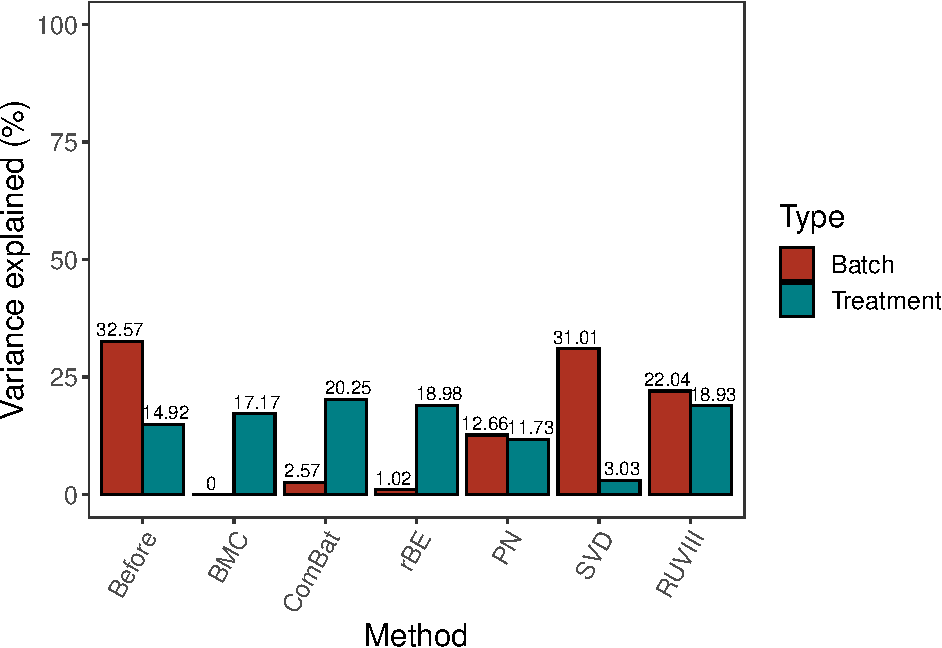
\includegraphics{Managing_batch_effects_files/figure-latex/unnamed-chunk-81-1.pdf}

Similar as results from sponge data, BMC, ComBat and removeBatchEffect
were more efficient at removing batch variation while preserving
treatment variation. ComBat removed relatively less batch variation
compared with the other two methods. Percentile normalisation did not
remove enough batch variation, nor preserve enough treatment variation
in AD data. RUVIII preserved enough treatment variation but did not
remove enough batch variation.

In sponge data, the results of BMC and removeBatchEffect are the same,
while in AD data, removeBatchEffect removed less batch variation but
preserved more treatment variation. This indicates some linear
correlation exists between the batch and treatment effects, which might
originate from the batch x treatment design.

\subsection{PVCA}\label{pvca}

PVCA can be applied as a validation method that complements pRDA, but it
requires 42 OTUs minimum. Therefore, it did not apply on sponge data.

\begin{Shaded}
\begin{Highlighting}[]
\CommentTok{# AD data}
\NormalTok{ad.PVCA.score <-}\StringTok{ }\KeywordTok{data.frame}\NormalTok{(}\DataTypeTok{Interaction =} \OtherTok{NA}\NormalTok{, }\DataTypeTok{Batch =} \OtherTok{NA}\NormalTok{, }
                           \DataTypeTok{Treatment =} \OtherTok{NA}\NormalTok{, }\DataTypeTok{Residuals =} \OtherTok{NA}\NormalTok{)}

\NormalTok{ad.Bat_Int.factors <-}\StringTok{ }\KeywordTok{data.frame}\NormalTok{(}\DataTypeTok{Batch =}\NormalTok{ ad.batch, }\DataTypeTok{Treatment =}\NormalTok{ ad.trt)}
\KeywordTok{rownames}\NormalTok{(ad.Bat_Int.factors) <-}\StringTok{ }\KeywordTok{rownames}\NormalTok{(ad.clr)}
\NormalTok{pdata <-}\StringTok{ }\KeywordTok{AnnotatedDataFrame}\NormalTok{(ad.Bat_Int.factors)}

\CommentTok{# before}
\NormalTok{ad.eset.X.before <-}\StringTok{ }\KeywordTok{new}\NormalTok{(}\StringTok{"ExpressionSet"}\NormalTok{, }\DataTypeTok{exprs =} \KeywordTok{t}\NormalTok{(ad.clr), }\DataTypeTok{phenoData =}\NormalTok{ pdata)}
\NormalTok{ad.pvcaObj.before <-}\StringTok{ }\KeywordTok{pvcaBatchAssess}\NormalTok{(ad.eset.X.before, }\KeywordTok{c}\NormalTok{(}\StringTok{'Batch'}\NormalTok{, }\StringTok{'Treatment'}\NormalTok{), }\FloatTok{0.6}\NormalTok{)}
\NormalTok{ad.values.before <-}\StringTok{ }\NormalTok{ad.pvcaObj.before}\OperatorTok{$}\NormalTok{dat}
\NormalTok{ad.PVCA.score[}\DecValTok{1}\NormalTok{, ] <-}\StringTok{ }\NormalTok{ad.values.before}

\CommentTok{# bmc}
\NormalTok{ad.eset.X.bmc <-}\StringTok{ }\KeywordTok{new}\NormalTok{(}\StringTok{"ExpressionSet"}\NormalTok{, }\DataTypeTok{exprs =} \KeywordTok{t}\NormalTok{(ad.bmc), }\DataTypeTok{phenoData =}\NormalTok{ pdata)}
\NormalTok{ad.pvcaObj.bmc <-}\StringTok{ }\KeywordTok{pvcaBatchAssess}\NormalTok{(ad.eset.X.bmc, }\KeywordTok{c}\NormalTok{(}\StringTok{'Batch'}\NormalTok{, }\StringTok{'Treatment'}\NormalTok{), }\FloatTok{0.6}\NormalTok{)}
\NormalTok{ad.values.bmc <-}\StringTok{ }\NormalTok{ad.pvcaObj.bmc}\OperatorTok{$}\NormalTok{dat}
\NormalTok{ad.PVCA.score[}\DecValTok{2}\NormalTok{, ] <-}\StringTok{ }\NormalTok{ad.values.bmc}


\CommentTok{# combat}

\NormalTok{ad.eset.X.combat <-}\StringTok{ }\KeywordTok{new}\NormalTok{(}\StringTok{"ExpressionSet"}\NormalTok{, }\DataTypeTok{exprs =} \KeywordTok{t}\NormalTok{(ad.combat), }\DataTypeTok{phenoData =}\NormalTok{ pdata)}
\NormalTok{ad.pvcaObj.combat <-}\StringTok{ }\KeywordTok{pvcaBatchAssess}\NormalTok{(ad.eset.X.combat, }\KeywordTok{c}\NormalTok{(}\StringTok{'Batch'}\NormalTok{, }\StringTok{'Treatment'}\NormalTok{), }\FloatTok{0.6}\NormalTok{)}
\NormalTok{ad.values.combat <-}\StringTok{ }\NormalTok{ad.pvcaObj.combat}\OperatorTok{$}\NormalTok{dat}
\NormalTok{ad.PVCA.score[}\DecValTok{3}\NormalTok{, ] <-}\StringTok{ }\NormalTok{ad.values.combat}

\CommentTok{# limma}

\NormalTok{ad.eset.X.limma <-}\StringTok{ }\KeywordTok{new}\NormalTok{(}\StringTok{"ExpressionSet"}\NormalTok{, }\DataTypeTok{exprs =} \KeywordTok{t}\NormalTok{(ad.limma), }\DataTypeTok{phenoData =}\NormalTok{ pdata)}
\NormalTok{ad.pvcaObj.limma <-}\StringTok{ }\KeywordTok{pvcaBatchAssess}\NormalTok{(ad.eset.X.limma, }\KeywordTok{c}\NormalTok{(}\StringTok{'Batch'}\NormalTok{, }\StringTok{'Treatment'}\NormalTok{), }\FloatTok{0.6}\NormalTok{)}
\NormalTok{ad.values.limma <-}\StringTok{ }\NormalTok{ad.pvcaObj.limma}\OperatorTok{$}\NormalTok{dat}
\NormalTok{ad.PVCA.score[}\DecValTok{4}\NormalTok{, ] <-}\StringTok{ }\NormalTok{ad.values.limma}


\CommentTok{# PN}

\NormalTok{ad.eset.X.percentile <-}\StringTok{ }\KeywordTok{new}\NormalTok{(}\StringTok{"ExpressionSet"}\NormalTok{, }\DataTypeTok{exprs =} \KeywordTok{t}\NormalTok{(ad.percentile), }
                            \DataTypeTok{phenoData =}\NormalTok{ pdata)}
\NormalTok{ad.pvcaObj.percentile <-}\StringTok{ }\KeywordTok{pvcaBatchAssess}\NormalTok{(ad.eset.X.percentile, }
                                         \KeywordTok{c}\NormalTok{(}\StringTok{'Batch'}\NormalTok{, }\StringTok{'Treatment'}\NormalTok{), }\FloatTok{0.6}\NormalTok{)}
\NormalTok{ad.values.percentile <-}\StringTok{ }\NormalTok{ad.pvcaObj.percentile}\OperatorTok{$}\NormalTok{dat}
\NormalTok{ad.PVCA.score[}\DecValTok{5}\NormalTok{, ] <-}\StringTok{ }\NormalTok{ad.values.percentile}


\CommentTok{# svd}

\NormalTok{ad.eset.X.svd <-}\StringTok{ }\KeywordTok{new}\NormalTok{(}\StringTok{"ExpressionSet"}\NormalTok{, }\DataTypeTok{exprs =} \KeywordTok{t}\NormalTok{(ad.svd), }\DataTypeTok{phenoData =}\NormalTok{ pdata)}
\NormalTok{ad.pvcaObj.svd <-}\StringTok{ }\KeywordTok{pvcaBatchAssess}\NormalTok{(ad.eset.X.svd, }\KeywordTok{c}\NormalTok{(}\StringTok{'Batch'}\NormalTok{, }\StringTok{'Treatment'}\NormalTok{), }\FloatTok{0.6}\NormalTok{)}
\NormalTok{ad.values.svd <-}\StringTok{ }\NormalTok{ad.pvcaObj.svd}\OperatorTok{$}\NormalTok{dat}
\NormalTok{ad.PVCA.score[}\DecValTok{6}\NormalTok{, ] <-}\StringTok{ }\NormalTok{ad.values.svd}


\CommentTok{# RUVIII}

\NormalTok{ad.eset.X.ruv <-}\StringTok{ }\KeywordTok{new}\NormalTok{(}\StringTok{"ExpressionSet"}\NormalTok{, }\DataTypeTok{exprs =} \KeywordTok{t}\NormalTok{(ad.ruvIII), }\DataTypeTok{phenoData =}\NormalTok{ pdata)}
\NormalTok{ad.pvcaObj.ruv <-}\StringTok{ }\KeywordTok{pvcaBatchAssess}\NormalTok{(ad.eset.X.ruv, }\KeywordTok{c}\NormalTok{(}\StringTok{'Batch'}\NormalTok{, }\StringTok{'Treatment'}\NormalTok{), }\FloatTok{0.6}\NormalTok{)}
\NormalTok{ad.values.ruv <-}\StringTok{ }\NormalTok{ad.pvcaObj.ruv}\OperatorTok{$}\NormalTok{dat}
\NormalTok{ad.PVCA.score[}\DecValTok{7}\NormalTok{, ] <-}\StringTok{ }\NormalTok{ad.values.ruv}

\KeywordTok{rownames}\NormalTok{(ad.PVCA.score) <-}\StringTok{ }\KeywordTok{c}\NormalTok{(}\StringTok{'Before'}\NormalTok{, }\StringTok{'BMC'}\NormalTok{, }\StringTok{'ComBat'}\NormalTok{, }\StringTok{'rBE'}\NormalTok{, }\StringTok{'PN'}\NormalTok{, }\StringTok{'SVD'}\NormalTok{, }\StringTok{'RUVIII'}\NormalTok{)}
\end{Highlighting}
\end{Shaded}

\begin{Shaded}
\begin{Highlighting}[]
\CommentTok{# merge results}
\NormalTok{ad.pvca.prop.val <-}\StringTok{ }\KeywordTok{c}\NormalTok{(ad.PVCA.score}\OperatorTok{$}\NormalTok{Batch, ad.PVCA.score}\OperatorTok{$}\NormalTok{Treatment)}

\CommentTok{# add batch, trt and method info}
\NormalTok{ad.pvca.prop <-}\StringTok{ }\KeywordTok{data.frame}\NormalTok{(}\DataTypeTok{prop =}\NormalTok{ ad.pvca.prop.val, }\DataTypeTok{prop.r =} \KeywordTok{round}\NormalTok{(ad.pvca.prop.val, }\DecValTok{2}\NormalTok{), }
                          \DataTypeTok{Method =} \KeywordTok{rep}\NormalTok{(}\KeywordTok{c}\NormalTok{(}\StringTok{'Before'}\NormalTok{, }\StringTok{'BMC'}\NormalTok{, }\StringTok{'ComBat'}\NormalTok{, }\StringTok{'rBE'}\NormalTok{, }
                                         \StringTok{'PN'}\NormalTok{, }\StringTok{'SVD'}\NormalTok{, }\StringTok{'RUVIII'}\NormalTok{), }\DecValTok{2}\NormalTok{), }
                          \DataTypeTok{Type =} \KeywordTok{rep}\NormalTok{(}\KeywordTok{c}\NormalTok{(}\StringTok{'Batch'}\NormalTok{, }\StringTok{'Treatment'}\NormalTok{), }\DataTypeTok{each =} \DecValTok{7}\NormalTok{))}

\CommentTok{# reorder levels}
\NormalTok{ad.pvca.prop}\OperatorTok{$}\NormalTok{Method <-}\StringTok{ }\KeywordTok{factor}\NormalTok{(ad.pvca.prop}\OperatorTok{$}\NormalTok{Method, }\DataTypeTok{levels =} \KeywordTok{unique}\NormalTok{(ad.pvca.prop}\OperatorTok{$}\NormalTok{Method))}

\KeywordTok{ggplot}\NormalTok{(}\DataTypeTok{data =}\NormalTok{ ad.pvca.prop, }\KeywordTok{aes}\NormalTok{(}\DataTypeTok{x =}\NormalTok{ Method, }\DataTypeTok{y =}\NormalTok{ prop, }\DataTypeTok{fill =}\NormalTok{ Type)) }\OperatorTok{+}\StringTok{ }
\StringTok{  }\KeywordTok{geom_bar}\NormalTok{(}\DataTypeTok{stat =} \StringTok{"identity"}\NormalTok{, }\DataTypeTok{position =} \StringTok{'dodge'}\NormalTok{, }\DataTypeTok{colour =} \StringTok{'black'}\NormalTok{) }\OperatorTok{+}\StringTok{ }
\StringTok{  }\KeywordTok{geom_text}\NormalTok{(}\DataTypeTok{data =}\NormalTok{ ad.pvca.prop, }\KeywordTok{aes}\NormalTok{(Method, prop }\OperatorTok{+}\StringTok{ }\FloatTok{0.03}\NormalTok{, }\DataTypeTok{label =}\NormalTok{ prop.r), }
            \DataTypeTok{position =} \KeywordTok{position_dodge}\NormalTok{(}\DataTypeTok{width =} \FloatTok{0.9}\NormalTok{), }\DataTypeTok{size =} \DecValTok{3}\NormalTok{) }\OperatorTok{+}\StringTok{ }\KeywordTok{theme_bw}\NormalTok{() }\OperatorTok{+}\StringTok{ }
\StringTok{  }\KeywordTok{labs}\NormalTok{(}\DataTypeTok{y =} \StringTok{"Weighted average proportion variance"}\NormalTok{) }\OperatorTok{+}\StringTok{ }
\StringTok{  }\KeywordTok{theme}\NormalTok{(}\DataTypeTok{axis.text.x =} \KeywordTok{element_text}\NormalTok{(}\DataTypeTok{angle =} \DecValTok{60}\NormalTok{, }\DataTypeTok{hjust =} \DecValTok{1}\NormalTok{), }
        \DataTypeTok{panel.grid =} \KeywordTok{element_blank}\NormalTok{(),}\DataTypeTok{axis.text =} \KeywordTok{element_text}\NormalTok{(}\DataTypeTok{size =} \DecValTok{12}\NormalTok{), }
        \DataTypeTok{axis.title =} \KeywordTok{element_text}\NormalTok{(}\DataTypeTok{size =} \DecValTok{15}\NormalTok{), }\DataTypeTok{legend.title =} \KeywordTok{element_text}\NormalTok{(}\DataTypeTok{size =} \DecValTok{15}\NormalTok{), }
        \DataTypeTok{legend.text =} \KeywordTok{element_text}\NormalTok{(}\DataTypeTok{size =} \DecValTok{12}\NormalTok{)) }\OperatorTok{+}\StringTok{ }\KeywordTok{scale_fill_hue}\NormalTok{(}\DataTypeTok{l =} \DecValTok{40}\NormalTok{) }\OperatorTok{+}\StringTok{ }\KeywordTok{ylim}\NormalTok{(}\DecValTok{0}\NormalTok{,}\DecValTok{1}\NormalTok{)}
\end{Highlighting}
\end{Shaded}

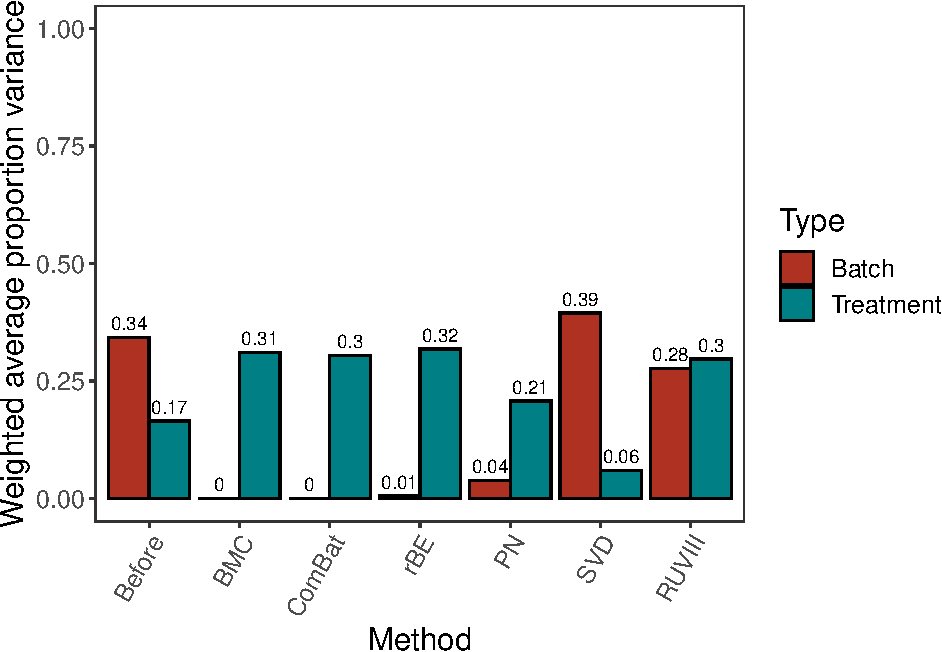
\includegraphics{Managing_batch_effects_files/figure-latex/unnamed-chunk-83-1.pdf}

Proportionally, BMC, ComBat and removeBatchEffect removed more of the
variance explained by batch and maintained more variance explained by
treatment than other methods in AD data.

\subsection{Silhouette coefficient}\label{silhouette-coefficient}

Finally we assess the quality of the clusters, based on either batch or
treatment information using the silhouette coefficient and the PC
components. This coefficient measures how cohesive a sample is to its
own cluster compared to other clusters. It has been adapted to assess
the consistency of sample groups based on treatment or batch effects.

The average silhouette coefficient width across all samples in one group
(batch \(\bar{s}_{b}\) or treatment \(\bar{s}_{t}\)) is calculated and
plotted here. If \(\bar{s}_{b}\) is close to \(0\) there is no batch
effect, and if \(\bar{s}_{t}\) is close to \(1\) or \(-1\) there is a
treatment effect.

\begin{Shaded}
\begin{Highlighting}[]
\CommentTok{# Sponge data}
\NormalTok{sponge.silh.before <-}\StringTok{ }\KeywordTok{calc.sil}\NormalTok{(sponge.pca.before}\OperatorTok{$}\NormalTok{variates}\OperatorTok{$}\NormalTok{X, }
                              \DataTypeTok{y1 =}\NormalTok{ sponge.batch, }\DataTypeTok{y2 =}\NormalTok{ sponge.trt, }
                              \DataTypeTok{name.y1 =} \StringTok{'Batch'}\NormalTok{, }\DataTypeTok{name.y2 =} \StringTok{'Tissue'}\NormalTok{)}
\NormalTok{sponge.silh.bmc <-}\StringTok{ }\KeywordTok{calc.sil}\NormalTok{(sponge.pca.bmc}\OperatorTok{$}\NormalTok{variates}\OperatorTok{$}\NormalTok{X, }
                           \DataTypeTok{y1 =}\NormalTok{ sponge.batch, }\DataTypeTok{y2 =}\NormalTok{ sponge.trt, }
                           \DataTypeTok{name.y1 =} \StringTok{'Batch'}\NormalTok{, }\DataTypeTok{name.y2 =} \StringTok{'Tissue'}\NormalTok{)}
\NormalTok{sponge.silh.combat <-}\StringTok{ }\KeywordTok{calc.sil}\NormalTok{(sponge.pca.combat}\OperatorTok{$}\NormalTok{variates}\OperatorTok{$}\NormalTok{X, }
                              \DataTypeTok{y1 =}\NormalTok{ sponge.batch, }\DataTypeTok{y2 =}\NormalTok{ sponge.trt, }
                              \DataTypeTok{name.y1 =} \StringTok{'Batch'}\NormalTok{, }\DataTypeTok{name.y2 =} \StringTok{'Tissue'}\NormalTok{)}
\NormalTok{sponge.silh.limma <-}\StringTok{ }\KeywordTok{calc.sil}\NormalTok{(sponge.pca.limma}\OperatorTok{$}\NormalTok{variates}\OperatorTok{$}\NormalTok{X, }
                             \DataTypeTok{y1 =}\NormalTok{ sponge.batch, }\DataTypeTok{y2 =}\NormalTok{ sponge.trt, }
                             \DataTypeTok{name.y1 =} \StringTok{'Batch'}\NormalTok{, }\DataTypeTok{name.y2 =} \StringTok{'Tissue'}\NormalTok{)}
\NormalTok{sponge.silh.percentile <-}\StringTok{ }\KeywordTok{calc.sil}\NormalTok{(sponge.pca.percentile}\OperatorTok{$}\NormalTok{variates}\OperatorTok{$}\NormalTok{X, }
                                  \DataTypeTok{y1 =}\NormalTok{ sponge.batch, }\DataTypeTok{y2 =}\NormalTok{ sponge.trt, }
                                  \DataTypeTok{name.y1 =} \StringTok{'Batch'}\NormalTok{, }\DataTypeTok{name.y2 =} \StringTok{'Tissue'}\NormalTok{)}
\NormalTok{sponge.silh.svd <-}\StringTok{ }\KeywordTok{calc.sil}\NormalTok{(sponge.pca.svd}\OperatorTok{$}\NormalTok{variates}\OperatorTok{$}\NormalTok{X, }
                           \DataTypeTok{y1 =}\NormalTok{ sponge.batch, }\DataTypeTok{y2 =}\NormalTok{ sponge.trt, }
                           \DataTypeTok{name.y1 =} \StringTok{'Batch'}\NormalTok{, }\DataTypeTok{name.y2 =} \StringTok{'Tissue'}\NormalTok{)}


\NormalTok{sponge.silh.plot <-}\StringTok{ }\KeywordTok{rbind}\NormalTok{(sponge.silh.before, sponge.silh.bmc, sponge.silh.combat, }
\NormalTok{                         sponge.silh.limma, sponge.silh.percentile, sponge.silh.svd)}
\NormalTok{sponge.silh.plot}\OperatorTok{$}\NormalTok{method <-}\StringTok{ }\KeywordTok{c}\NormalTok{(}\KeywordTok{rep}\NormalTok{(}\StringTok{'Before'}\NormalTok{, }\KeywordTok{nrow}\NormalTok{(sponge.silh.before)), }
                            \KeywordTok{rep}\NormalTok{(}\StringTok{'BMC'}\NormalTok{, }\KeywordTok{nrow}\NormalTok{(sponge.silh.bmc)),}
                            \KeywordTok{rep}\NormalTok{(}\StringTok{'ComBat'}\NormalTok{, }\KeywordTok{nrow}\NormalTok{(sponge.silh.combat)),}
                            \KeywordTok{rep}\NormalTok{(}\StringTok{'rBE'}\NormalTok{, }\KeywordTok{nrow}\NormalTok{(sponge.silh.limma)),}
                            \KeywordTok{rep}\NormalTok{(}\StringTok{'PN'}\NormalTok{, }\KeywordTok{nrow}\NormalTok{(sponge.silh.percentile)),}
                            \KeywordTok{rep}\NormalTok{(}\StringTok{'SVD'}\NormalTok{, }\KeywordTok{nrow}\NormalTok{(sponge.silh.svd))}
\NormalTok{)}
\NormalTok{sponge.silh.plot}\OperatorTok{$}\NormalTok{method <-}\StringTok{ }\KeywordTok{factor}\NormalTok{(sponge.silh.plot}\OperatorTok{$}\NormalTok{method, }
                                 \DataTypeTok{levels =} \KeywordTok{unique}\NormalTok{(sponge.silh.plot}\OperatorTok{$}\NormalTok{method))}
\NormalTok{sponge.silh.plot}\OperatorTok{$}\NormalTok{Cluster <-}\StringTok{ }\KeywordTok{factor}\NormalTok{(sponge.silh.plot}\OperatorTok{$}\NormalTok{Cluster, }
                                   \DataTypeTok{levels =} \KeywordTok{unique}\NormalTok{(sponge.silh.plot}\OperatorTok{$}\NormalTok{Cluster))}
\NormalTok{sponge.silh.plot}\OperatorTok{$}\NormalTok{Type <-}\StringTok{ }\KeywordTok{factor}\NormalTok{(sponge.silh.plot}\OperatorTok{$}\NormalTok{Type, }
                                \DataTypeTok{levels =} \KeywordTok{unique}\NormalTok{(sponge.silh.plot}\OperatorTok{$}\NormalTok{Type))}


\KeywordTok{ggplot}\NormalTok{(sponge.silh.plot, }\KeywordTok{aes}\NormalTok{(}\DataTypeTok{x =}\NormalTok{ Type, }\DataTypeTok{y =}\NormalTok{ silh.coeff, }\DataTypeTok{color =}\NormalTok{ Cluster, }\DataTypeTok{shape =}\NormalTok{ Type)) }\OperatorTok{+}\StringTok{ }
\StringTok{  }\KeywordTok{geom_point}\NormalTok{() }\OperatorTok{+}\StringTok{ }\KeywordTok{facet_grid}\NormalTok{(}\DataTypeTok{cols =} \KeywordTok{vars}\NormalTok{(method)) }\OperatorTok{+}\StringTok{ }\KeywordTok{theme_bw}\NormalTok{() }\OperatorTok{+}\StringTok{ }
\StringTok{  }\KeywordTok{theme}\NormalTok{(}\DataTypeTok{axis.text.x =} \KeywordTok{element_text}\NormalTok{(}\DataTypeTok{angle =} \DecValTok{60}\NormalTok{, }\DataTypeTok{hjust =} \DecValTok{1}\NormalTok{), }
        \DataTypeTok{strip.text =} \KeywordTok{element_text}\NormalTok{(}\DataTypeTok{size =} \DecValTok{12}\NormalTok{), }\DataTypeTok{panel.grid =} \KeywordTok{element_blank}\NormalTok{(), }
        \DataTypeTok{axis.text =} \KeywordTok{element_text}\NormalTok{(}\DataTypeTok{size =} \DecValTok{12}\NormalTok{), }\DataTypeTok{axis.title =} \KeywordTok{element_text}\NormalTok{(}\DataTypeTok{size =} \DecValTok{15}\NormalTok{),}
        \DataTypeTok{legend.title =} \KeywordTok{element_text}\NormalTok{(}\DataTypeTok{size =} \DecValTok{15}\NormalTok{), }\DataTypeTok{legend.text =} \KeywordTok{element_text}\NormalTok{(}\DataTypeTok{size =} \DecValTok{12}\NormalTok{)) }\OperatorTok{+}\StringTok{ }
\StringTok{  }\KeywordTok{scale_color_manual}\NormalTok{(}\DataTypeTok{values =} \KeywordTok{c}\NormalTok{(}\StringTok{'#388ECC'}\NormalTok{,}\StringTok{'#F68B33'}\NormalTok{,}\StringTok{'#F0E442'}\NormalTok{,}\StringTok{'#D55E00'}\NormalTok{)) }\OperatorTok{+}\StringTok{ }
\StringTok{  }\KeywordTok{labs}\NormalTok{(}\DataTypeTok{x =} \StringTok{'Type'}\NormalTok{, }\DataTypeTok{y =} \StringTok{'Silhouette Coefficient'}\NormalTok{, }\DataTypeTok{name =} \StringTok{'Type'}\NormalTok{) }
\end{Highlighting}
\end{Shaded}

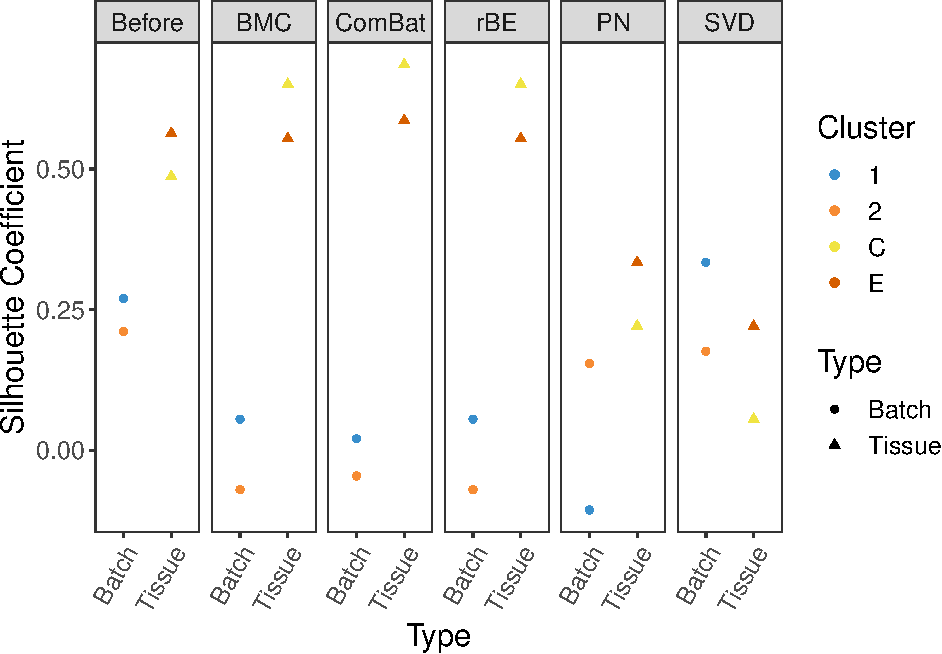
\includegraphics{Managing_batch_effects_files/figure-latex/unnamed-chunk-84-1.pdf}

\(\bar{s}_{b}\) of different batches in sponge data decreased to \(0\)
after correction with BMC, ComBat and removeBatchEffect, while
\(\bar{s}_{t}\) of different tissues increased or maintained at the same
level as before correction.

We also calculate the silhouette coefficients for AD data.

\begin{Shaded}
\begin{Highlighting}[]
\CommentTok{# AD data}
\NormalTok{ad.silh.before <-}\StringTok{ }\KeywordTok{calc.sil}\NormalTok{(ad.pca.before}\OperatorTok{$}\NormalTok{variates}\OperatorTok{$}\NormalTok{X, }\DataTypeTok{y1 =}\NormalTok{ ad.batch, }
                          \DataTypeTok{y2 =}\NormalTok{ ad.trt, }\DataTypeTok{name.y1 =} \StringTok{'Batch'}\NormalTok{, }\DataTypeTok{name.y2 =} \StringTok{'Treatment'}\NormalTok{)}
\NormalTok{ad.silh.bmc <-}\StringTok{ }\KeywordTok{calc.sil}\NormalTok{(ad.pca.bmc}\OperatorTok{$}\NormalTok{variates}\OperatorTok{$}\NormalTok{X, }\DataTypeTok{y1 =}\NormalTok{ ad.batch, }
                       \DataTypeTok{y2 =}\NormalTok{ ad.trt, }\DataTypeTok{name.y1 =} \StringTok{'Batch'}\NormalTok{, }\DataTypeTok{name.y2 =} \StringTok{'Treatment'}\NormalTok{)}
\NormalTok{ad.silh.combat <-}\StringTok{ }\KeywordTok{calc.sil}\NormalTok{(ad.pca.combat}\OperatorTok{$}\NormalTok{variates}\OperatorTok{$}\NormalTok{X, }\DataTypeTok{y1 =}\NormalTok{ ad.batch, }
                          \DataTypeTok{y2 =}\NormalTok{ ad.trt, }\DataTypeTok{name.y1 =} \StringTok{'Batch'}\NormalTok{, }\DataTypeTok{name.y2 =} \StringTok{'Treatment'}\NormalTok{)}
\NormalTok{ad.silh.limma <-}\StringTok{ }\KeywordTok{calc.sil}\NormalTok{(ad.pca.limma}\OperatorTok{$}\NormalTok{variates}\OperatorTok{$}\NormalTok{X, }\DataTypeTok{y1 =}\NormalTok{ ad.batch, }
                         \DataTypeTok{y2 =}\NormalTok{ ad.trt, }\DataTypeTok{name.y1 =} \StringTok{'Batch'}\NormalTok{, }\DataTypeTok{name.y2 =} \StringTok{'Treatment'}\NormalTok{)}
\NormalTok{ad.silh.percentile <-}\StringTok{ }\KeywordTok{calc.sil}\NormalTok{(ad.pca.percentile}\OperatorTok{$}\NormalTok{variates}\OperatorTok{$}\NormalTok{X, }\DataTypeTok{y1 =}\NormalTok{ ad.batch, }
                              \DataTypeTok{y2 =}\NormalTok{ ad.trt, }\DataTypeTok{name.y1 =} \StringTok{'Batch'}\NormalTok{, }\DataTypeTok{name.y2 =} \StringTok{'Treatment'}\NormalTok{)}
\NormalTok{ad.silh.svd <-}\StringTok{ }\KeywordTok{calc.sil}\NormalTok{(ad.pca.svd}\OperatorTok{$}\NormalTok{variates}\OperatorTok{$}\NormalTok{X, }\DataTypeTok{y1 =}\NormalTok{ ad.batch, }
                       \DataTypeTok{y2 =}\NormalTok{ ad.trt, }\DataTypeTok{name.y1 =} \StringTok{'Batch'}\NormalTok{, }\DataTypeTok{name.y2 =} \StringTok{'Treatment'}\NormalTok{)}
\NormalTok{ad.silh.ruv <-}\StringTok{ }\KeywordTok{calc.sil}\NormalTok{(ad.pca.ruv}\OperatorTok{$}\NormalTok{variates}\OperatorTok{$}\NormalTok{X, }\DataTypeTok{y1 =}\NormalTok{ ad.batch, }
                       \DataTypeTok{y2 =}\NormalTok{ ad.trt, }\DataTypeTok{name.y1 =} \StringTok{'Batch'}\NormalTok{, }\DataTypeTok{name.y2 =} \StringTok{'Treatment'}\NormalTok{)}


\NormalTok{ad.silh.plot <-}\StringTok{ }\KeywordTok{rbind}\NormalTok{(ad.silh.before, ad.silh.bmc, ad.silh.combat, }
\NormalTok{                     ad.silh.limma, ad.silh.percentile, ad.silh.svd, ad.silh.ruv)}
\NormalTok{ad.silh.plot}\OperatorTok{$}\NormalTok{method <-}\StringTok{ }\KeywordTok{c}\NormalTok{(}\KeywordTok{rep}\NormalTok{(}\StringTok{'Before'}\NormalTok{, }\KeywordTok{nrow}\NormalTok{(ad.silh.before)), }
                        \KeywordTok{rep}\NormalTok{(}\StringTok{'BMC'}\NormalTok{, }\KeywordTok{nrow}\NormalTok{(ad.silh.bmc)),}
                        \KeywordTok{rep}\NormalTok{(}\StringTok{'ComBat'}\NormalTok{, }\KeywordTok{nrow}\NormalTok{(ad.silh.combat)),}
                        \KeywordTok{rep}\NormalTok{(}\StringTok{'rBE'}\NormalTok{, }\KeywordTok{nrow}\NormalTok{(ad.silh.limma)),}
                        \KeywordTok{rep}\NormalTok{(}\StringTok{'PN'}\NormalTok{, }\KeywordTok{nrow}\NormalTok{(ad.silh.percentile)),}
                        \KeywordTok{rep}\NormalTok{(}\StringTok{'SVD'}\NormalTok{, }\KeywordTok{nrow}\NormalTok{(ad.silh.svd)),}
                        \KeywordTok{rep}\NormalTok{(}\StringTok{'RUVIII'}\NormalTok{, }\KeywordTok{nrow}\NormalTok{(ad.silh.ruv))}
\NormalTok{)}
\NormalTok{ad.silh.plot}\OperatorTok{$}\NormalTok{method <-}\StringTok{ }\KeywordTok{factor}\NormalTok{(ad.silh.plot}\OperatorTok{$}\NormalTok{method, }\DataTypeTok{levels =} \KeywordTok{unique}\NormalTok{(ad.silh.plot}\OperatorTok{$}\NormalTok{method))}
\NormalTok{ad.silh.plot}\OperatorTok{$}\NormalTok{Cluster <-}\StringTok{ }\KeywordTok{factor}\NormalTok{(ad.silh.plot}\OperatorTok{$}\NormalTok{Cluster, }\DataTypeTok{levels =} \KeywordTok{unique}\NormalTok{(ad.silh.plot}\OperatorTok{$}\NormalTok{Cluster))}
\NormalTok{ad.silh.plot}\OperatorTok{$}\NormalTok{Type <-}\StringTok{ }\KeywordTok{factor}\NormalTok{(ad.silh.plot}\OperatorTok{$}\NormalTok{Type, }\DataTypeTok{levels =} \KeywordTok{unique}\NormalTok{(ad.silh.plot}\OperatorTok{$}\NormalTok{Type))}

\KeywordTok{ggplot}\NormalTok{(ad.silh.plot, }\KeywordTok{aes}\NormalTok{(}\DataTypeTok{x =}\NormalTok{ Type, }\DataTypeTok{y =}\NormalTok{ silh.coeff, }\DataTypeTok{color =}\NormalTok{ Cluster, }\DataTypeTok{shape =}\NormalTok{ Type)) }\OperatorTok{+}\StringTok{ }
\StringTok{  }\KeywordTok{geom_point}\NormalTok{() }\OperatorTok{+}\StringTok{ }\KeywordTok{facet_grid}\NormalTok{(}\DataTypeTok{cols =} \KeywordTok{vars}\NormalTok{(method)) }\OperatorTok{+}\StringTok{ }\KeywordTok{theme_bw}\NormalTok{() }\OperatorTok{+}\StringTok{ }
\StringTok{  }\KeywordTok{theme}\NormalTok{(}\DataTypeTok{axis.text.x =} \KeywordTok{element_text}\NormalTok{(}\DataTypeTok{angle =} \DecValTok{60}\NormalTok{, }\DataTypeTok{hjust =} \DecValTok{1}\NormalTok{), }
        \DataTypeTok{strip.text =} \KeywordTok{element_text}\NormalTok{(}\DataTypeTok{size =} \DecValTok{12}\NormalTok{), }\DataTypeTok{panel.grid =} \KeywordTok{element_blank}\NormalTok{(), }
        \DataTypeTok{axis.text =} \KeywordTok{element_text}\NormalTok{(}\DataTypeTok{size =} \DecValTok{10}\NormalTok{), }\DataTypeTok{axis.title =} \KeywordTok{element_text}\NormalTok{(}\DataTypeTok{size =} \DecValTok{15}\NormalTok{),}
        \DataTypeTok{legend.title =} \KeywordTok{element_text}\NormalTok{(}\DataTypeTok{size =} \DecValTok{15}\NormalTok{), }\DataTypeTok{legend.text =} \KeywordTok{element_text}\NormalTok{(}\DataTypeTok{size =} \DecValTok{12}\NormalTok{)) }\OperatorTok{+}\StringTok{ }
\StringTok{  }\KeywordTok{scale_color_manual}\NormalTok{(}\DataTypeTok{values =} \KeywordTok{c}\NormalTok{(}\StringTok{'#388ECC'}\NormalTok{, }\StringTok{'#F68B33'}\NormalTok{, }\StringTok{'#C2C2C2'}\NormalTok{, }\StringTok{'#009E73'}\NormalTok{, }
                                \StringTok{'#CC79A7'}\NormalTok{, }\StringTok{'#0072B2'}\NormalTok{, }\StringTok{'#999999'}\NormalTok{)) }\OperatorTok{+}\StringTok{ }
\StringTok{  }\KeywordTok{labs}\NormalTok{(}\DataTypeTok{x =} \StringTok{'Type'}\NormalTok{, }\DataTypeTok{y =} \StringTok{'Silhouette Coefficient'}\NormalTok{, }\DataTypeTok{name =} \StringTok{'Type'}\NormalTok{) }
\end{Highlighting}
\end{Shaded}

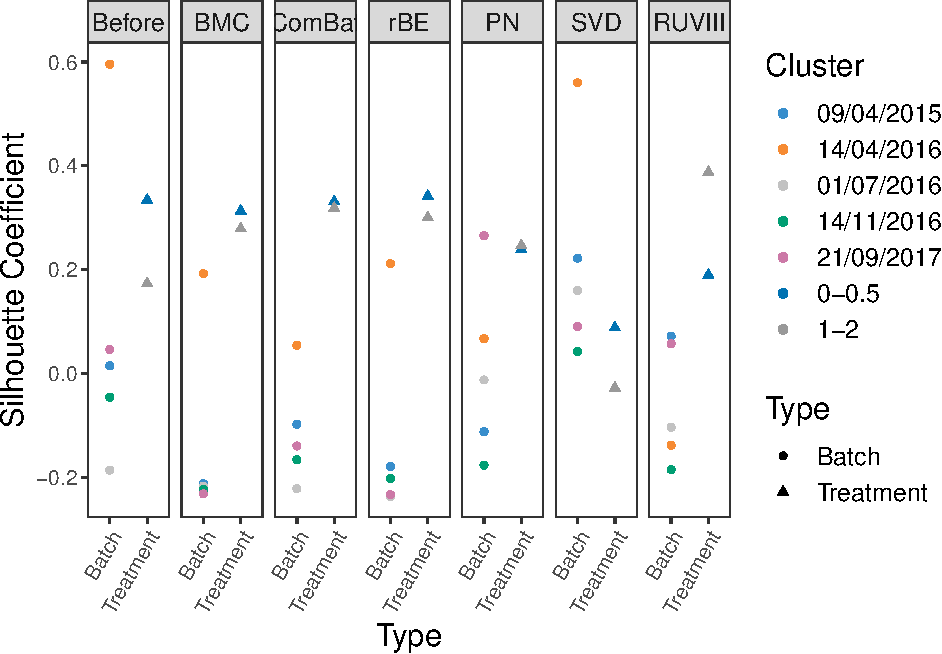
\includegraphics{Managing_batch_effects_files/figure-latex/unnamed-chunk-85-1.pdf}

In AD data that includes five batches, the interpretation of the results
is challenging. After correction, BMC, ComBat, removeBatchEffect,
percentile normalisation and RUVIII decreased the batch silhouette
coefficients for the batch dated 14/04/2016, but increased the
coefficients for the other batches. Therefore it is difficult to assess
the efficiency of these methods in this particular case.

\chapter{Assessment of the nature of batch effects}\label{simu}

\section{Simulations}\label{simulations}

\subsection{Mean = 5, and unequal
variance}\label{mean-5-and-unequal-variance}

`Systematic' refers to homogeneous change amongst all microbial
variables (OTUs) due to having the same source of variation. We
illustrate this concept in a linear model framework where batch and
treatment regression coefficients are estimated simultaneously on each
OTU. For a given batch effect and a given OTU, we can formulate the
systematic assumption as:

\[\beta_{j} \sim N(\mu,\sigma^{2})\]

where \(\beta_{j}\) is the batch regression coefficient of OTU\(_{j}\)
(\(j = 1,...,p\)). Here we consider the simplest case of a linear model
with one batch predictor, but this formulation could be extended to a
model with multiple batch predictors where the batch regression
coefficients can represent more than two batch levels. In a univariate
model that tests each OTU individually, then the distribution of the
batch coefficients of all OTUs is Gaussian with a mean \(\mu\), and
standard deviation \(\sigma\). This indicates that the batch effect has
a similar, though not necessarily identical, influence on all OTUs.

To illustrate the type of batch effects, we simulated a set of data with
50 samples and 10,000 OTUs each, based on the simulation approach from
\citep{gagnon2013removing}.

The dataset with a systematic batch effect:

\begin{itemize}
\tightlist
\item
  \(\beta_{j} \sim N(5,1^{2})\) for \(j=1,...,p\) OTUs;\\
\item
  \(\sigma_{j} \sim N(0,2^{2})\) for \(j=1,...,p\) OTUs; This variance
  per OTU is aimed to simulate data as realistically as possible.\\
\item
  \(\beta_{ij} \sim N(\beta_{j}, \sigma_{j}^{2})\) for \(i = 1,...,n\)
  samples.
\end{itemize}

\begin{Shaded}
\begin{Highlighting}[]
\CommentTok{# Create the simulated data}
\NormalTok{m <-}\StringTok{ }\DecValTok{50}
\NormalTok{n <-}\StringTok{ }\DecValTok{10000}
\NormalTok{nc <-}\StringTok{ }\DecValTok{1000} \CommentTok{# negative controls without treatment effects}
\NormalTok{p <-}\StringTok{ }\DecValTok{1}
\NormalTok{k <-}\StringTok{ }\DecValTok{1}
\NormalTok{ctl <-}\StringTok{ }\KeywordTok{rep}\NormalTok{(}\OtherTok{FALSE}\NormalTok{, n)}
\NormalTok{ctl[}\DecValTok{1}\OperatorTok{:}\NormalTok{nc] <-}\StringTok{ }\OtherTok{TRUE}
\CommentTok{# treatment effect}
\NormalTok{X <-}\StringTok{ }\KeywordTok{matrix}\NormalTok{(}\KeywordTok{c}\NormalTok{(}\KeywordTok{rep}\NormalTok{(}\DecValTok{0}\NormalTok{, }\KeywordTok{floor}\NormalTok{(m}\OperatorTok{/}\DecValTok{2}\NormalTok{)), }\KeywordTok{rep}\NormalTok{(}\DecValTok{1}\NormalTok{, }\KeywordTok{ceiling}\NormalTok{(m}\OperatorTok{/}\DecValTok{2}\NormalTok{))), m, p)}
\NormalTok{beta <-}\StringTok{ }\KeywordTok{matrix}\NormalTok{(}\KeywordTok{rnorm}\NormalTok{(p}\OperatorTok{*}\NormalTok{n, }\DecValTok{5}\NormalTok{, }\DecValTok{1}\NormalTok{), p, n) }\CommentTok{#treatment coefficients}
\NormalTok{beta[ ,ctl] <-}\StringTok{ }\DecValTok{0}
\CommentTok{# batch effect}
\NormalTok{W <-}\StringTok{ }\KeywordTok{as.matrix}\NormalTok{(}\KeywordTok{rep}\NormalTok{(}\DecValTok{0}\NormalTok{, m), m, k)}
\NormalTok{W[}\KeywordTok{c}\NormalTok{(}\DecValTok{1}\OperatorTok{:}\DecValTok{12}\NormalTok{,}\DecValTok{38}\OperatorTok{:}\DecValTok{50}\NormalTok{), }\DecValTok{1}\NormalTok{] <-}\StringTok{  }\DecValTok{1}
\NormalTok{alpha <-}\StringTok{ }\KeywordTok{matrix}\NormalTok{(}\KeywordTok{rnorm}\NormalTok{(k}\OperatorTok{*}\NormalTok{n, }\DecValTok{5}\NormalTok{, }\DecValTok{1}\NormalTok{), k, n)}
\NormalTok{Y_alpha <-}\StringTok{ }\KeywordTok{sapply}\NormalTok{(alpha, }\ControlFlowTok{function}\NormalTok{(alpha)\{}\KeywordTok{rnorm}\NormalTok{(m, }\DataTypeTok{mean =}\NormalTok{  alpha, }
                                              \KeywordTok{abs}\NormalTok{(}\KeywordTok{rnorm}\NormalTok{(}\DecValTok{1}\NormalTok{, }\DataTypeTok{mean =} \DecValTok{0}\NormalTok{, }\DataTypeTok{sd =} \DecValTok{2}\NormalTok{)))\})}
\NormalTok{YY_alpha <-}\StringTok{ }\KeywordTok{apply}\NormalTok{(Y_alpha, }\DecValTok{2}\NormalTok{, }\ControlFlowTok{function}\NormalTok{(x)\{x}\OperatorTok{*}\NormalTok{W\})}

\NormalTok{epsilon <-}\StringTok{ }\KeywordTok{matrix}\NormalTok{(}\KeywordTok{rnorm}\NormalTok{(m}\OperatorTok{*}\NormalTok{n, }\DecValTok{0}\NormalTok{, }\DecValTok{1}\NormalTok{), m, n)}
\NormalTok{Y <-}\StringTok{ }\NormalTok{X}\OperatorTok\NormalTok{beta }\OperatorTok{+}\StringTok{ }\NormalTok{YY_alpha }\OperatorTok{+}\StringTok{ }\NormalTok{epsilon}


\CommentTok{# estimate batch coefficient for each OTU}
\NormalTok{w.cof <-}\StringTok{ }\KeywordTok{c}\NormalTok{()}
\ControlFlowTok{for}\NormalTok{(i }\ControlFlowTok{in} \DecValTok{1}\OperatorTok{:}\KeywordTok{ncol}\NormalTok{(Y))\{}
\NormalTok{  res <-}\StringTok{ }\KeywordTok{lm}\NormalTok{(Y[ ,i] }\OperatorTok{~}\StringTok{ }\NormalTok{X }\OperatorTok{+}\StringTok{ }\NormalTok{W)}
\NormalTok{  sum.res <-}\StringTok{ }\KeywordTok{summary}\NormalTok{(res)}
\NormalTok{  w.cof[i] <-}\StringTok{ }\NormalTok{sum.res}\OperatorTok{$}\NormalTok{coefficients[}\DecValTok{3}\NormalTok{,}\DecValTok{1}\NormalTok{]}
\NormalTok{\}}

\KeywordTok{par}\NormalTok{(}\DataTypeTok{mfrow =} \KeywordTok{c}\NormalTok{(}\DecValTok{2}\NormalTok{,}\DecValTok{2}\NormalTok{))}
\KeywordTok{hist}\NormalTok{(w.cof,}\DataTypeTok{col =} \StringTok{'gray'}\NormalTok{)}
\KeywordTok{plot}\NormalTok{(}\KeywordTok{density}\NormalTok{(w.cof))}
\KeywordTok{qqnorm}\NormalTok{(w.cof)}
\KeywordTok{qqline}\NormalTok{(w.cof, }\DataTypeTok{col =} \StringTok{'red'}\NormalTok{)}
\KeywordTok{par}\NormalTok{(}\DataTypeTok{mfrow =} \KeywordTok{c}\NormalTok{(}\DecValTok{1}\NormalTok{,}\DecValTok{1}\NormalTok{))}
\end{Highlighting}
\end{Shaded}

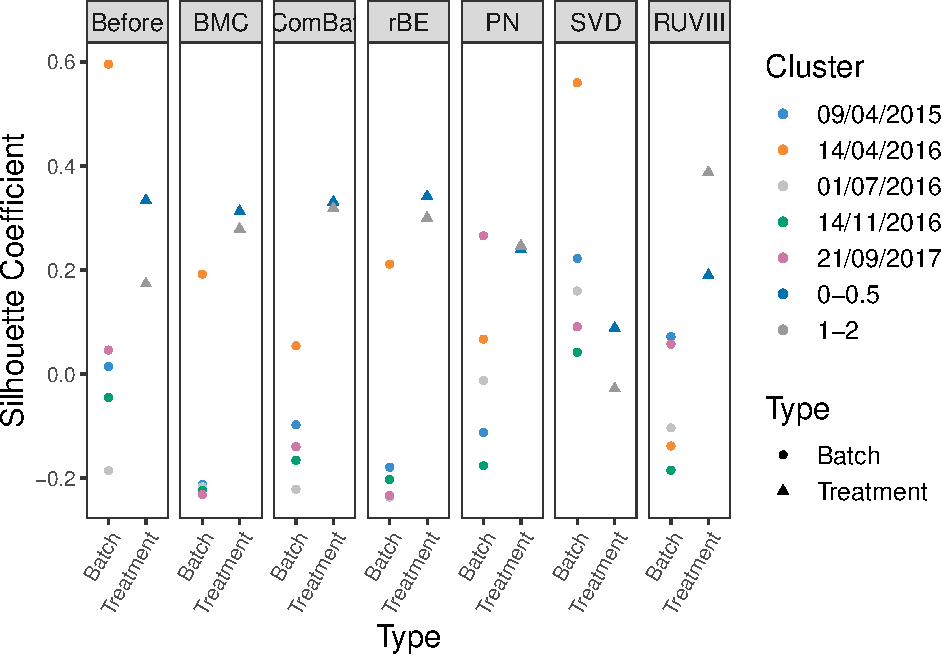
\includegraphics{Managing_batch_effects_files/figure-latex/unnamed-chunk-86-1.pdf}

The histogram, density plot and quantile--quantile plot are plotted
using estimated batch regression coefficients \(\hat{\beta}_{j}\) for
each OTU \(j\). These plots display the distribution of batch
coefficients is very close to normal, indicating a systematic batch
effect.

\subsection{Mean = 0 or 5, and unequal
variance}\label{mean-0-or-5-and-unequal-variance}

Non-systematic batch effects have a heterogeneous influence on microbial
variables. Using a linear model framework, as described previously, we
can formulate this non-systematic assumption as:

\[
\beta'_{j} \sim 
  \begin{cases} 
    N(0,\delta^{2}) & \text{for OTUs with no batch effect,} \\
    N(\mu,\sigma^{2}) & \text{for OTUs with batch effect.}
  \end{cases}
\]

Therefore, the batch regression coefficients \(\beta'_{j}\) may follow
skewed distributions with several modes.

The dataset with non-systematic batch effect:

\begin{itemize}
\tightlist
\item
  \(\beta'_{t} \sim N(0,1^{2})\) and \(\beta'_{k} \sim N(5,1^{2})\) for
  \(t=1,...,T\) OTUs, \(k=1,...,K\) OTUs and \(T=\frac{3}{4}p\),
  \(K=\frac{1}{4}p\);\\
\item
  \(\sigma'_{j} \sim N(0,2^{2})\) for \(j=1,...,p\) OTUs;\\
\item
  \(\beta'_{ij} \sim N(\beta'_{j}, \sigma_{j}^{'2})\) for
  \(i = 1,...,n\) samples.
\end{itemize}

\begin{Shaded}
\begin{Highlighting}[]
\CommentTok{# Create the simulated data}
\NormalTok{m <-}\StringTok{ }\DecValTok{50}
\NormalTok{n <-}\StringTok{ }\DecValTok{10000}
\NormalTok{nc <-}\StringTok{ }\DecValTok{1000} \CommentTok{# negative controls without treatment effects}
\NormalTok{p <-}\StringTok{ }\DecValTok{1}
\NormalTok{k <-}\StringTok{ }\DecValTok{1}
\NormalTok{ctl <-}\StringTok{ }\KeywordTok{rep}\NormalTok{(}\OtherTok{FALSE}\NormalTok{, n)}
\NormalTok{ctl[}\DecValTok{1}\OperatorTok{:}\NormalTok{nc] <-}\StringTok{ }\OtherTok{TRUE}
\CommentTok{# treatment effect}
\NormalTok{X <-}\StringTok{ }\KeywordTok{matrix}\NormalTok{(}\KeywordTok{c}\NormalTok{(}\KeywordTok{rep}\NormalTok{(}\DecValTok{0}\NormalTok{, }\KeywordTok{floor}\NormalTok{(m}\OperatorTok{/}\DecValTok{2}\NormalTok{)), }\KeywordTok{rep}\NormalTok{(}\DecValTok{1}\NormalTok{, }\KeywordTok{ceiling}\NormalTok{(m}\OperatorTok{/}\DecValTok{2}\NormalTok{))), m, p)}
\NormalTok{beta <-}\StringTok{ }\KeywordTok{matrix}\NormalTok{(}\KeywordTok{rnorm}\NormalTok{(p}\OperatorTok{*}\NormalTok{n, }\DecValTok{5}\NormalTok{, }\DecValTok{1}\NormalTok{), p, n) }\CommentTok{#treatment coefficients}
\NormalTok{beta[ ,ctl] <-}\StringTok{ }\DecValTok{0}
\CommentTok{# batch effect}
\NormalTok{W <-}\StringTok{ }\KeywordTok{as.matrix}\NormalTok{(}\KeywordTok{rep}\NormalTok{(}\DecValTok{0}\NormalTok{, m), m, k)}
\NormalTok{W[}\KeywordTok{c}\NormalTok{(}\DecValTok{1}\OperatorTok{:}\DecValTok{12}\NormalTok{,}\DecValTok{38}\OperatorTok{:}\DecValTok{50}\NormalTok{), }\DecValTok{1}\NormalTok{] <-}\StringTok{  }\DecValTok{1}
\NormalTok{alpha2 <-}\StringTok{ }\KeywordTok{matrix}\NormalTok{(}\KeywordTok{sample}\NormalTok{(}\KeywordTok{c}\NormalTok{(}\KeywordTok{rnorm}\NormalTok{(k}\OperatorTok{*}\NormalTok{(}\DecValTok{3}\OperatorTok{*}\NormalTok{n}\OperatorTok{/}\DecValTok{4}\NormalTok{), }\DecValTok{0}\NormalTok{, }\DecValTok{1}\NormalTok{),}\KeywordTok{rnorm}\NormalTok{(k}\OperatorTok{*}\NormalTok{(n}\OperatorTok{/}\DecValTok{4}\NormalTok{), }\DecValTok{5}\NormalTok{, }\DecValTok{1}\NormalTok{)), n), k, n)}
\NormalTok{Y_alpha2 <-}\StringTok{ }\KeywordTok{sapply}\NormalTok{(alpha2, }\ControlFlowTok{function}\NormalTok{(alpha)\{}\KeywordTok{rnorm}\NormalTok{(m, }\DataTypeTok{mean =}\NormalTok{  alpha, }
                                                \DataTypeTok{sd =} \KeywordTok{abs}\NormalTok{(}\KeywordTok{rnorm}\NormalTok{(}\DecValTok{1}\NormalTok{, }\DataTypeTok{mean =} \DecValTok{0}\NormalTok{, }\DataTypeTok{sd =} \DecValTok{2}\NormalTok{)))\})}
\NormalTok{YY_alpha2 <-}\StringTok{ }\KeywordTok{apply}\NormalTok{(Y_alpha2, }\DecValTok{2}\NormalTok{, }\ControlFlowTok{function}\NormalTok{(x)\{x}\OperatorTok{*}\NormalTok{W\})}

\NormalTok{epsilon <-}\StringTok{ }\KeywordTok{matrix}\NormalTok{(}\KeywordTok{rnorm}\NormalTok{(m}\OperatorTok{*}\NormalTok{n, }\DecValTok{0}\NormalTok{, }\DecValTok{1}\NormalTok{), m, n)}
\NormalTok{Y2 <-}\StringTok{ }\NormalTok{X}\OperatorTok\NormalTok{beta }\OperatorTok{+}\StringTok{ }\NormalTok{YY_alpha2 }\OperatorTok{+}\StringTok{ }\NormalTok{epsilon}




\NormalTok{w.cof2 <-}\StringTok{ }\KeywordTok{c}\NormalTok{()}
\ControlFlowTok{for}\NormalTok{(i }\ControlFlowTok{in} \DecValTok{1}\OperatorTok{:}\KeywordTok{ncol}\NormalTok{(Y2))\{}
\NormalTok{  res <-}\StringTok{ }\KeywordTok{lm}\NormalTok{(Y2[ ,i] }\OperatorTok{~}\StringTok{ }\NormalTok{X }\OperatorTok{+}\StringTok{ }\NormalTok{W)}
\NormalTok{  sum.res <-}\StringTok{ }\KeywordTok{summary}\NormalTok{(res)}
\NormalTok{  w.cof2[i] <-}\StringTok{ }\NormalTok{sum.res}\OperatorTok{$}\NormalTok{coefficients[}\DecValTok{3}\NormalTok{,}\DecValTok{1}\NormalTok{]}
\NormalTok{\}}

\KeywordTok{par}\NormalTok{(}\DataTypeTok{mfrow =} \KeywordTok{c}\NormalTok{(}\DecValTok{2}\NormalTok{,}\DecValTok{2}\NormalTok{))}
\KeywordTok{hist}\NormalTok{(w.cof2, }\DataTypeTok{col =} \StringTok{'gray'}\NormalTok{)}
\KeywordTok{plot}\NormalTok{(}\KeywordTok{density}\NormalTok{(w.cof2))}
\KeywordTok{qqnorm}\NormalTok{(w.cof2)}
\KeywordTok{qqline}\NormalTok{(w.cof2, }\DataTypeTok{col =} \StringTok{'red'}\NormalTok{)}
\KeywordTok{par}\NormalTok{(}\DataTypeTok{mfrow =} \KeywordTok{c}\NormalTok{(}\DecValTok{1}\NormalTok{,}\DecValTok{1}\NormalTok{))}
\end{Highlighting}
\end{Shaded}

\includegraphics{Managing_batch_effects_files/figure-latex/unnamed-chunk-87-1.pdf}

The histogram, density plot and quantile--quantile plot are plotted
using estimated batch regression coefficients \(\hat{\beta}_{j}\) for
each OTU \(j\), showing a bi-modal distribution. This distribution
indicates a non-systematic batch effect.

\textbf{We observed similar patterns in our real case studies,
suggesting that the batch effects are mixed with multiple sources and
are non-systematic (see the examples below).}

\section{Real data}\label{real-data}

We also estimate the batch regression coefficients for each OTU in real
datasets to assess the nature of batch effects.

\subsection{Sponge data}\label{sponge-data}

\begin{Shaded}
\begin{Highlighting}[]
\NormalTok{sponge.b.coeff <-}\StringTok{ }\KeywordTok{c}\NormalTok{()}
\ControlFlowTok{for}\NormalTok{(i }\ControlFlowTok{in} \DecValTok{1}\OperatorTok{:}\KeywordTok{ncol}\NormalTok{(sponge.tss.clr))\{}
\NormalTok{  res <-}\StringTok{ }\KeywordTok{lm}\NormalTok{(sponge.tss.clr[ ,i] }\OperatorTok{~}\StringTok{ }\NormalTok{sponge.trt }\OperatorTok{+}\StringTok{ }\NormalTok{sponge.batch)}
\NormalTok{  sum.res <-}\StringTok{ }\KeywordTok{summary}\NormalTok{(res)}
\NormalTok{  sponge.b.coeff[i] <-}\StringTok{ }\NormalTok{sum.res}\OperatorTok{$}\NormalTok{coefficients[}\DecValTok{3}\NormalTok{,}\DecValTok{1}\NormalTok{]}
\NormalTok{\}}

\KeywordTok{par}\NormalTok{(}\DataTypeTok{mfrow =} \KeywordTok{c}\NormalTok{(}\DecValTok{2}\NormalTok{,}\DecValTok{2}\NormalTok{))}
\KeywordTok{hist}\NormalTok{(sponge.b.coeff,}\DataTypeTok{col =} \StringTok{'gray'}\NormalTok{)}
\KeywordTok{plot}\NormalTok{(}\KeywordTok{density}\NormalTok{(sponge.b.coeff))}
\KeywordTok{qqnorm}\NormalTok{(sponge.b.coeff)}
\KeywordTok{qqline}\NormalTok{(sponge.b.coeff, }\DataTypeTok{col=}\StringTok{'red'}\NormalTok{)}
\KeywordTok{par}\NormalTok{(}\DataTypeTok{mfrow =} \KeywordTok{c}\NormalTok{(}\DecValTok{1}\NormalTok{,}\DecValTok{1}\NormalTok{))}
\end{Highlighting}
\end{Shaded}

\includegraphics{Managing_batch_effects_files/figure-latex/unnamed-chunk-88-1.pdf}

In sponge data, the histogram, density plot and quantile--quantile plot
are also plotted using estimated batch regression coefficients
\(\hat{\beta}_{j}\) for each OTU \(j\). The bi-modal distribution
indicates a non-systematic batch effect, which is similar as the results
from simulation with non-systematic batch effects.

\subsection{AD data}\label{ad-data}

\begin{Shaded}
\begin{Highlighting}[]
\NormalTok{ad.b.coeff <-}\StringTok{ }\KeywordTok{c}\NormalTok{()}
\NormalTok{ad.batch.relevel <-}\StringTok{ }\KeywordTok{relevel}\NormalTok{(ad.batch, }\StringTok{'01/07/2016'}\NormalTok{)}
\ControlFlowTok{for}\NormalTok{(i }\ControlFlowTok{in} \DecValTok{1}\OperatorTok{:}\KeywordTok{ncol}\NormalTok{(ad.clr))\{}
\NormalTok{  res <-}\StringTok{ }\KeywordTok{lm}\NormalTok{(ad.clr[,i] }\OperatorTok{~}\StringTok{ }\NormalTok{ad.trt }\OperatorTok{+}\StringTok{ }\NormalTok{ad.batch.relevel)}
\NormalTok{  sum.res <-}\StringTok{ }\KeywordTok{summary}\NormalTok{(res)}
\NormalTok{  ad.b.coeff[i] <-}\StringTok{ }\NormalTok{sum.res}\OperatorTok{$}\NormalTok{coefficients[}\DecValTok{4}\NormalTok{,}\DecValTok{1}\NormalTok{]}
\NormalTok{\}}

\KeywordTok{par}\NormalTok{(}\DataTypeTok{mfrow =} \KeywordTok{c}\NormalTok{(}\DecValTok{2}\NormalTok{,}\DecValTok{2}\NormalTok{))}
\KeywordTok{hist}\NormalTok{(ad.b.coeff,}\DataTypeTok{col =} \StringTok{'gray'}\NormalTok{)}
\KeywordTok{plot}\NormalTok{(}\KeywordTok{density}\NormalTok{(ad.b.coeff))}
\KeywordTok{qqnorm}\NormalTok{(ad.b.coeff)}
\KeywordTok{qqline}\NormalTok{(ad.b.coeff, }\DataTypeTok{col=}\StringTok{'red'}\NormalTok{)}
\KeywordTok{par}\NormalTok{(}\DataTypeTok{mfrow =} \KeywordTok{c}\NormalTok{(}\DecValTok{1}\NormalTok{,}\DecValTok{1}\NormalTok{))}
\end{Highlighting}
\end{Shaded}

\includegraphics{Managing_batch_effects_files/figure-latex/unnamed-chunk-89-1.pdf}

We observe similar results in AD data. The distribution of estimated
batch regression coefficients is not normal. The batch effects therefore
are non-systematic.

\bibliography{book.bib,packages.bib}


\end{document}
